\documentclass[11pt]{mytustyle}  % default square logo 
%\documentclass[12pt,beltcrest]{ociamthesis} % use old belt crest logo
%\documentclass[12pt,shieldcrest]{ociamthesis} % use older shield crest logo

%load any additional packages
\usepackage{amssymb}

%input macros (i.e. write your own macros file called mymacros.tex 
%and uncomment the next line)
%\include{mymacros}

\title{Diamond as a versatile\\[1ex]     %your thesis title,
        beam loss detector}   %note \\[1ex] is a line break in the title

\author{Matev\v{z} \v{C}erv}             %your name
%\supervisor{Dr. Erich Griesmayer}             %supervisor

\college{Vienna University of Technology}  %your college

%\renewcommand{\submittedtext}{change the default text here if needed}
\degree{Doctor of technical sciences}     %the degree
\degreedate{Geneva 2015}         %the degree date

%end the preamble and start the document
\begin{document}

%this baselineskip gives sufficient line spacing for an examiner to easily
%markup the thesis with comments
\baselineskip=18pt plus1pt

%set the number of sectioning levels that get number and appear in the contents
\setcounter{secnumdepth}{3}
\setcounter{tocdepth}{3}


\maketitle                  % create a title page from the preamble info
%\begin{dedication}
This thesis is dedicated to\\
my parents \\

\end{dedication}        % include a dedication.tex file
%\begin{acknowledgements}
plenty of waffle, plenty of waffle, plenty of waffle, plenty of waffle,
plenty of waffle, plenty of waffle, plenty of waffle, plenty of waffle.
\end{acknowledgements}   % include an acknowledgements.tex file
%\begin{abstract}

This document contains 

\end{abstract}          % include the abstract

\begin{romanpages}          % start roman page numbering
\tableofcontents            % generate and include a table of contents
\listoffigures              % generate and include a list of figures
\end{romanpages}            % end roman page numbering

%now include the files of latex for each of the chapters etc
%\begin{abstract}

This document contains 

\end{abstract}
%\begin{acknowledgements}
My special appreciation and thanks go to to my advisors Dr. Heinz Pernegger and Dr. Erich Griesmayer. Your support of my work has been invaluable. In the past four years I have grown professionally as well as personally. By accepting me to the Marie Curie TALENT programme you allowed me to embark on a life-changing and eye-opening journey, which will definitely have a major impact on me in the years to come. I will take this opportunity to acknowledge that this work position at CERN was included in the Work Package 2 of the Marie Curie Early Initial Training Network Fellowship of the European Community�s Seventh Framework Programme under contract number (PITN-GA-2011-289161- TALENT).

I would also like to thank Andrej and Marko. Without your selfless support during my early days as a researcher I would be where I am today. You gave me an insight into joys of particle physics research (i.e. playing around with expensive hardware), which gave rise to my increased interest in involvement with CERN.

Next I would like to extend my gratitude to my dear colleagues in the work groups: Jennifer, Sonia, Karola, Timon, Christian, Branislav, Simon, Doug, Malte, Hendrik and Pavel. You stood by my side in my days of sorrow when the measurement setup decided to punish me with abstract errors, you helped me fight the battles against segfaults, corrected my sloppy writing and, most importantly, you made sure we never ran out of much needed coffee and banter in the office. 

A big shout-out to all my Geneva friends. Our friendship has left a big mark on my life and I will never forget the fun, the music and all the great moments we spent together.

I am deeply thankful to my family for their love and support. Vida, Roman, you always believed in me and encouraged me on the path I chose and for this I will be forever indebted to you. Miha, Klemen, Ana, Meta, Zala, Julija, you are the best. Finally, I would like to thank Ur\v{s}ka. You have walked the path alongside me and supported me and made these years together ever so enjoyable.

Matev\v{z}	

\end{acknowledgements}

%\begin{dedication}
This thesis is dedicated to\\
my parents \\

\end{dedication}

% ---------------------------------------------------------------------------------------------------------------
\chapter{Introduction}
\label{ch:intro}
% ---------------------------------------------------------------------------------------------------------------


The aim of the thesis is to present and discuss applications of diamond based particle detectors. 

The introductory chapter paints a picture of the current state of particle physics research. It presents some of the research institutes that are active in this field, pushing the boundaries of human knowledge further. It explains their goals and the means with which they are achieving them. Next section describes particle detectors in a broad sense -- their history and the types existing now. One type in particular -- a diamond detector -- is then described more in detail.

The second chapter discusses the properties of diamond detectors. First it explains the detector chain into individual parts and describes them in detail -- sensors, amplifiers, digitisers and signal processing units. Second, it contains information about energy resolution in diamond, the analog and digital noise contribution, etc. Third, it presents the principles of signal formation, starting with the famous Shockley-Ramo theorem and building from there. It uses the theorem to show that different types of radiation induce different electrical signal shapes.

The base laid down in the second chapter is complemented in the third where the measurements are presented and the results discussed. The chapter focuses on charge measurement stability with respect to irradiation damage.

Building on the understanding of the behaviour of the diamond, two applications were developed. The fourth chapter describes the Diamond Beam Monitor, a detector that makes use of the diamond's charge measurement capabilities and its high radiation hardness. This detector has been installed in one of the largest particle physics experiments in the world and is currently taking data. Here, its development process is presented: the quality control procedures during assembly and installation, its performance in the test environment and some recent experimental data.

The final and most important chapter describes the real-time application for particle identification. Here the shape of the current signal of the diamond sensor is used to discriminate different types of radiation in real time. The chapter includes the description of the device's logic and algorithms, experimental results and applications in neutron monitoring.


 




% ---------------------------------------------------------------------------------------------------------------
\clearpage
\section{Fundamental research}
\label{sec:fundphy}
% ---------------------------------------------------------------------------------------------------------------
This section gives a short overview of the institutes and collaborations carrying out fundamental physics research. The facilities were used for the research carried out in this thesis. 

The aim of fundamental research is to define scientific theories and verify them to improve our understanding of the universe. It does not in itself focus on applying this research by developing products and is not meant to create a direct return on investment. Instead, it expands the overall knowledge of the human kind - by making the results freely available to the general public.

Particle physics research peers into the smallest constituents of the universe, dissecting the atoms into quarks and electrons, catching cosmic rays and figuring out what dark matter is made up of. Particle physicists want to explain the phenomena surrounding us by studying the fundamental particles and the mechanisms governing their interactions. By understanding this, we would be able to answer difficult questions; How did the universe begin? What is the invisible force (dark matter, dark energy) pushing the galaxies apart from each other? Where does mass come from? Why is there almost no antimatter in the universe? In this effort, scientists have formed several theories. One of them, the Standard Model of particles, is currently the best theory to describe the constituents of matter and their interactions.

\begin{description}
\item[The Standard Model]
(SM) is a physics theory developed in the 1970's~\cite{Novaes:1999yn}. It was designed to explain the current experimental results. As such, it was also able to predict new discoveries and was a driving force for the scientists to invest time and money in developing new experiments. To date, it is by far the most established and verified physics theory. It explains how the basic building blocks of matter -- \emph{fermions} -- interact with each other via mediators of interactions called \emph{bosons}.  
\begin{figure}[!t]
\centering
\includegraphics[width=0.9\textwidth]{01_introduction/pics/sm}
\caption{Standard model \cite{Dominguez:2002395}.}
\label{fig:sm}
\end{figure}
There are two main families of fermions - \emph{quarks} and \emph{leptons}, as shown in figure~\ref{fig:sm}. Each group consists of six members divided into three \emph{generations}, the first being the lightest and most stable and the last the heaviest -- unstable. The nature around us is made up of the stable particles -- those from the second or third generations can only be found in cosmic rays or produced artificially using particle accelerators.

Quarks have a spin of 1/2 and a charge of either +2/3 (up, charm, top)  or -1/3  (down, strange, bottom) while the leptons have a spin of 1/2  and a charge of either 1 (electron, muon, tau) or 0 (electron neutrino, muon neutrino, tau neutrino). Leptons only exist individually -- they do not cluster. Quarks, however, immediately form a cluster of either two (unstable), three (more stable) or five (unstable). Two up and one down quark make up a proton whereas two down and one up quark make up a neutron.

In addition to fermions, each particle has its corresponding antiparticle -- a particle with the same mass but the opposite charge. If an antiparticle hits a particle, they annihilate each other, producing energy in form of photons. 

Bosons are the carriers of force, mediating weak (W$^+$, W$^-$ and Z bosons), strong (gluons) and electromagnetic (photons) interactions. The weak interaction is responsible for the radioactive decay of subatomic particles, thus playing an essential role in nuclear fission -- a process taking place in the stars. The electromagnetic interaction works at a macroscopic level -- it allows particles to interact via electric and magnetic fields. The strong interaction is effective at distances of a femtometer and it governs how quarks interact and bind with each other. An additional boson is the Higgs boson and was discovered at CERN in 2012~\cite{}. It is a representation of the Higgs mechanism, which gives rise to the mass (or lack thereof) of all the particles in the Standard Model.
\end{description}

\subsection{CERN}
CERN (European Centre for Nuclear Research)~\cite{CERN:00000} is the largest particle physics laboratory in the world, straddling the Swiss-French border just outside Geneva. It was established in 1954 to bring the war-torn Europe together by means of fundamental scientific research. Today, its 22 member state countries and several observer states contribute approximately 1~billion CHF annually to fund the research and development. More than 10000 scientists, engineers, technicians, students and others from all around the globe work at CERN on many projects in research fields ranging from particle to nuclear physics. The scope is to probe the fundamental structure of the universe and to understand the mechanisms governing it. Therefore CERN's main function is to provide the infrastructure for high-energy physics experiments. These are carried out using large machines called particle accelerators. These instruments boost beams of particles to high energies before making them collide with each other or with stationary targets. The resulting collisions are recorded by particle detectors and later analysed by physicists. To carry out research on the smallest constituents of matter, their dynamics and structure, very high energies are needed. This is why the most powerful accelerators are used for fundamental research. The largest accelerators at CERN are the Proton Synchrotron~\cite{}, the Super Proton Synchrotron~\cite{Mills:133232} and the Large Hadron Collider~\cite{}, described in~\ref{subsec:lhc}.

\subsection{Particle accelerators}
A particle accelerator is a machine that accelerates beams of charged particles like protons, electrons, ions etc. It generates electric fields that add kinetic energy to the particles, speeding them up. It then uses magnets to retain them within a defined trajectory and inside the evacuated beam pipe. The trajectory can be either linear (linear accelerators) or circular (circular or cyclic accelerators). The advantage of the latter ones is that they can accelerate particles many times while keeping them in orbit.

Particle accelerators are used in numerous fields ranging from fundamental and material research, cancer treatment to industrial applications, such as biomedicine and material processing. Several types of accelerators exist: electrostatic accelerators, linear accelerators (LINACs), cyclotrons, synchrocyclotrons, synchrotrons, synchrotron radiation sources and fixed-field alternating gradient accelerators (FFAGs).

\begin{description}
\item[The Large Hadron Collider]
\label{subsec:lhc}
(LHC, figure~\ref{fig:lhc}) at CERN is the largest particle collider in the world. It was build between 1998 and 2008 and was first successfully started in 2010 and operated stably until 2013 when it underwent a two years long upgrade. Its second operational cycle started at the beginning of 2015.

The LHC is a 27~km long circular machine set up in a tunnel deep under the surface, ranging from 50 to 175~m below ground. It accelerates two proton beams to the energy of 6.5~TeV per beam before it makes them to collide with each other with the energy of 13~TeV at four different points around its circumference. 
\begin{figure}[!t]
\centering
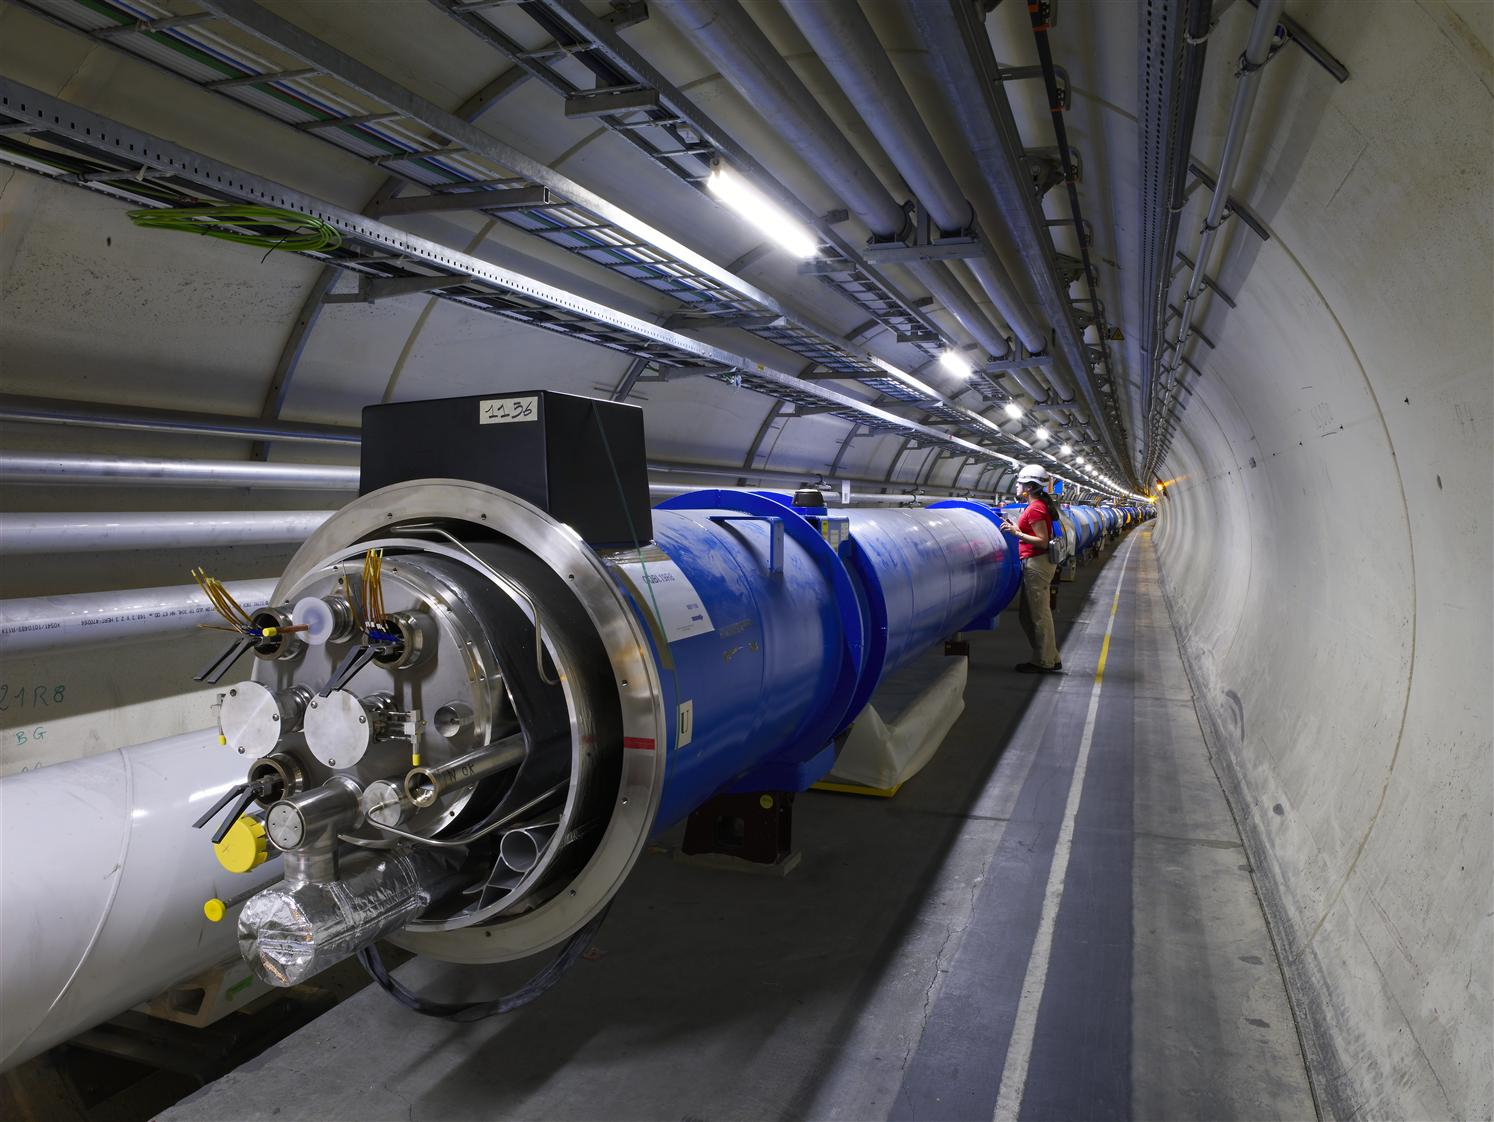
\includegraphics[width=0.9\textwidth]{01_introduction/pics/lhc}
\caption{The Large Hadron Collider \cite{Maximilien:1324852}.}
\label{fig:lhc}
\end{figure}
The hair-thin particle beams travel inside two evacuated pipes with a $\sim$5~cm radius. Coils made up of a superconductive material are wound up around the pipes in special patterns. When cooled down to -271 \textdegree C using liquid helium, they become superconductive; the resistivity of the material drops significantly, minimising the heat dissipation despite high electric currents. These produce strong magnetic fields which bend the particles and keep them in a circular trajectory. The particles are accelerated when traversing the radio-frequency (RF) cavities with the RF frequency of 400~MHz. This oscillating frequency creates buckets -- compartments for bunches of highly energetic particles -- which are 2.5~ns long. Only one out of ten buckets is filled, so the bunches are spaced at 25~ns. This defines the machine's clock (40~MHz) as well as the maximum rate of collisions - the bunches travelling in the opposite direction cross at the intersections up to 40~million times per second. Currently around 20 collisions occur during every bunch crossing, yielding the maximum collision rate of the order of $10^9$~s$^{-1}$. The number of collisions will further increase in the following years; the number of particles in every bunch will be increased and the transverse spread of the bunches will be decreased, squeezing the bunches further. The density will therefore be increased, which will in turn increase the collision probability -- the cross-section. The original design number of collisions accumulated over the years of operation is presented in the form of integrated luminosity~\cite{} and is of the order of 300~fb$^{-1}$ (inverse femtobarn). After the planned upgrades in 2020, the High-Luminosity LHC~\cite{} will achieve up to 3000~fb$^{-1}$.
\end{description}

\subsection{The ATLAS experiment}
ATLAS (short for A Toroidal Lhc ApparatuS, figure~\ref{fig:atlas})~\cite{} is a particle physics experiment at CERN. Its purpose is to verify current theories and to search for new discoveries by observing and analysing high energy proton-proton collisions produced by the LHC. It is the biggest experiment at CERN by dimensions (45~m in length and 26~m in height) and the number of people involved (more than 3000 physicists and engineers).
\begin{figure}[!t]
\centering
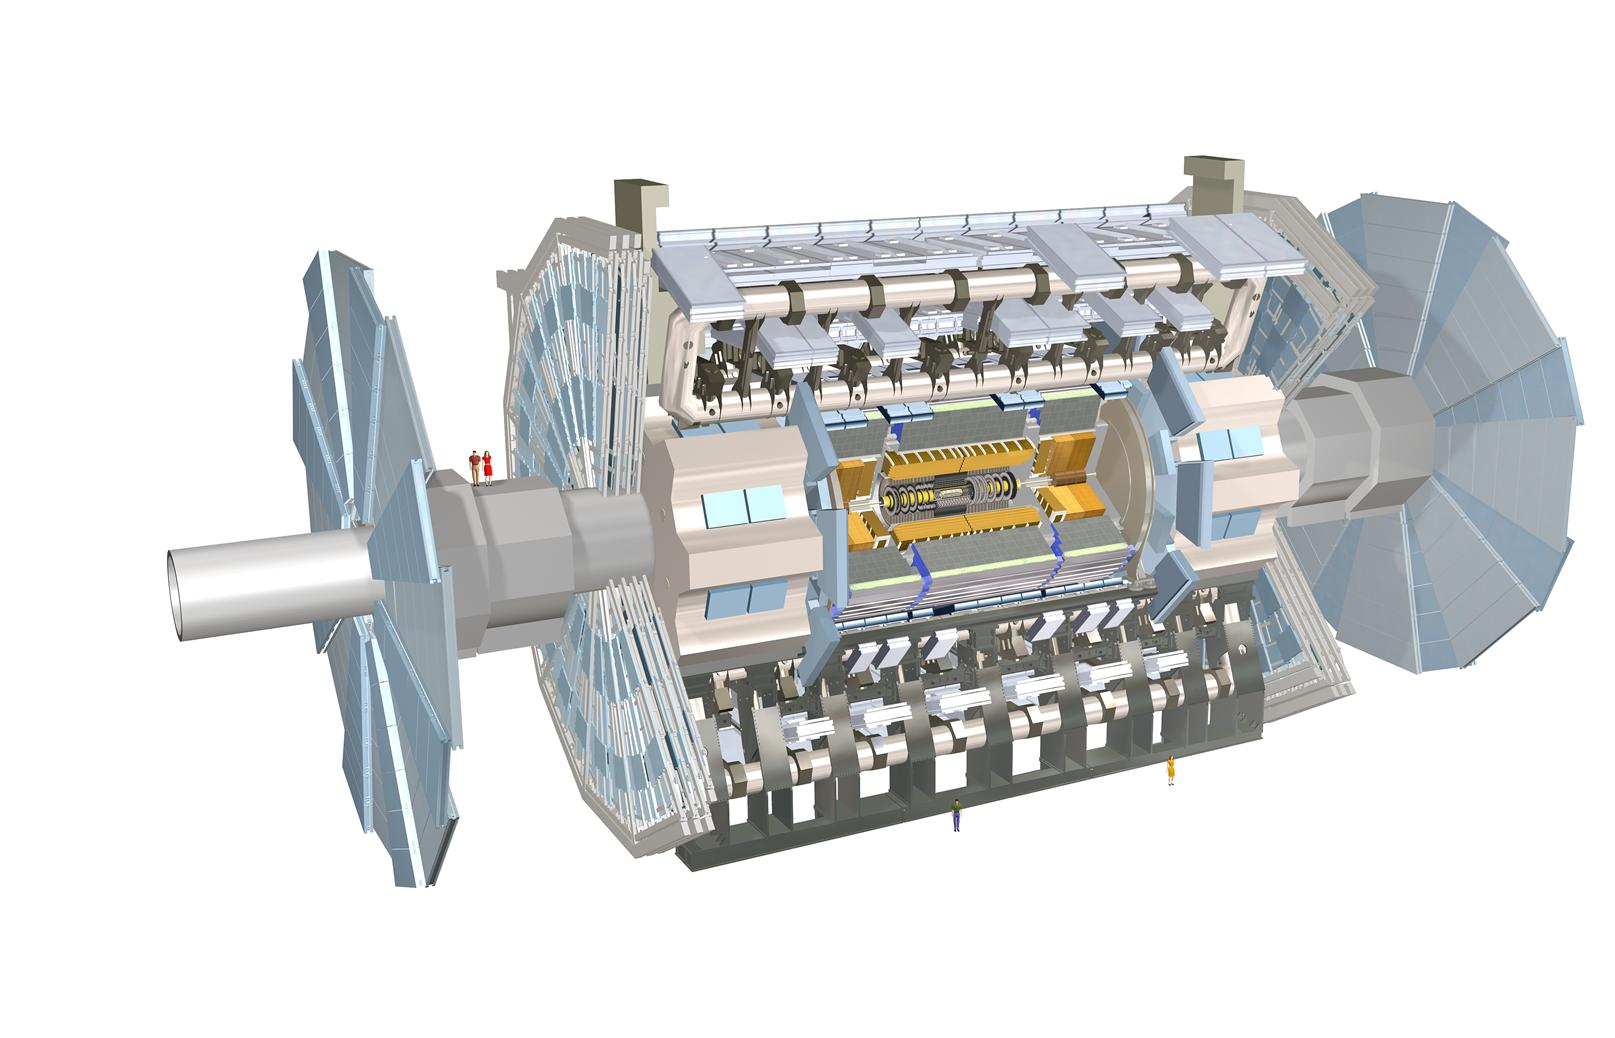
\includegraphics[width=0.9\textwidth]{01_introduction/pics/atlas3}
\caption{The ATLAS Experiment \cite{Pequenao:1095924}.}
\label{fig:atlas}
\end{figure}
The ATLAS experiment consists of a number of detectors, each designed to measure a specific property of the particles and photons produced during the collision. The closest to the collision point is the Inner Detector (ID), which consists of several layers of highly spatially segmented semiconductor sensors recording single points of the incident particles. These points are later reconstructed into particle tracks. In addition, a strong magnetic field of 2~T curves the paths of the charged particles, which in turn allows the ID to identify an individual particle's charge and momentum. The next two parts are the electromagnetic and tile calorimeter. These detectors weigh a few thousand tonnes and measure the energy of the particles that are stopped in the material. The only particles that make it through the calorimeters are muons. These are detected by the Muon Spectrometer, a set of large detector plates placed all around the calorimeters. Last is the superconductive magnet, which provides the magnetic field through the entire ATLAS except the ID, which already has its own magnets. To sum up, the Inner Detector measures the charge and momenta of the particles, the calorimeters measure their energies, the Muon Spectrometer measures muons and the magnets provide magnetic fields, which curve the trajectories of the charged particles, allowing for identification of particle momentum.

A complex Trigger and Data Acquisition system (TDAQ) is in place to distribute the clock signal, configure the detectors, trigger them and handle the output data. They are then stored at the CERN computer centre and distributed across the globe by means of the GRID -- a distributed data analysis and data storage system.

The ATLAS detector has been designed to measure every collision taking place in its core. With 25~ns between collisions, this makes up 40~million collisions per second. In reality, the maximum achievable rate is about 300~kHz. The recorded collision is called an event. Every event holds information from all the detector channels within ATLAS. With $\sim$$10^6$ channels, an event size is approximately 10~MB. At the maximum achievable rate this means a data rate of up to 3~TB/s. To reduce the amount of data stored a special classification system with a complex trigger logic is in place to decide which events should be stored and analysed further. It is programmed to decide in the order of tens of microseconds after an event whether it is potentially interesting or not. If so, the system triggers the readout of the entire detector. This way the recorded event rate is reduced from 300~kHz to $\sim$500~Hz.


\subsection{Atominstitut, Vienna}
Atominstitut (ATI)~\cite{AtomInst:00000}, an institute for atomic and subatomic physics, was established in 1958 in Vienna as an inter-university institute. It currently houses around 200 people involved in a broad range of research fields: quantum, particle, neutron, nuclear, radiation and reactor physics, quantum optics etc. Its central facility is a TRIGA MARK II neutron reactor (described in detail below). 

As of 2002 the ATI is part of the University of Technology in Vienna.


\begin{description}
\begin{figure}[!t]
\centering
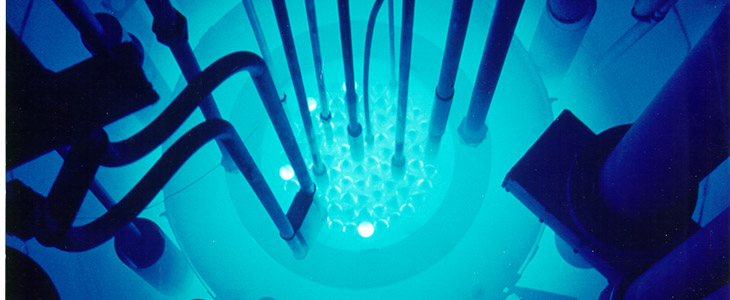
\includegraphics[width=0.9\textwidth]{01_introduction/pics/triga}
\caption{The TRIGA MARK II neutron reactor \cite{GeneralAtomics}.}
\label{fig:triga}
\end{figure}
\item[TRIGA MARK II neutron reactor]~\cite{Triga:00000} is a reactor of a swimming-pool type used for training, research and isotope production. It is one of 40 such reactors worldwide, produced by the Californian company General Atomic in the early 60's. It is capable of continuous operation at a maximum output power of 250~kW. 
The reactor core consists of 3~kg of 20~\% enriched uranium ($^{235}$U). The fuel moderator rods are mostly made up of zirconium with low percentage of hydrogen and uranium. Both the core and the rods are immersed in a pool of water as shown in figure~\ref{fig:triga} for the purpose of cooling and radiation protection. The surrounding concrete walls are 2~m wide with an added graphite layer for improved shielding. Four main experimental beam holes are placed radially through the walls. All exits are heavily shielded to prevent radiation damage to people, but still leaving enough space to set up experiments. Apart from the beam holes, there are several other exits and components, e.g. a thermal column for generation of thermal (low energetic) neutrons.


\end{description}

% MORE!



\subsection{n-ToF}
n-ToF (or neutron time-of-flight)~\cite{NTOF:00000} is a scientific collaboration with the aim of studying neutron-nucleus interactions. Over 30 institutes and universities are currently active members of this collaboration, among them Atominstitut in Vienna. n-ToF is also a facility at CERN where the experiments are carried out in a 200 m long experimental area. The knowledge stemming from the experimental results can then be applied in various fields ranging from nuclear technology and cancer therapy to astrophysics.

A pulsed beam of highly energetic protons (20~GeV/c) is produced by the Proton Synchrotron (PS) and aimed at a fixed lead spallation target. Each proton hitting the target produces around 300 neutrons of various energies. Initially highly energetic neutrons are slowed down by the target and by a slab of water placed behind it. This broadens their energy spectrum, which then ranges from meV (thermal neutrons) to GeV (fast neutrons). The neutrons are then collimated and sent through a 185~m long evacuated pipe to the experimental area, where they are made to collide with another target or a sample. The radiation resulting from the collisions is detected by a set of dedicated detectors around the interaction point, as shown in figure~\ref{fig:ntof}. Having different energies, neutrons travel with different speeds, highly energetic ones reaching the target faster than those with low energies. The analysis of collisions with a precise timing allows for a determination of the interaction probability with the sample material as a function of incident neutron energy.
\begin{figure}[!t]
\centering
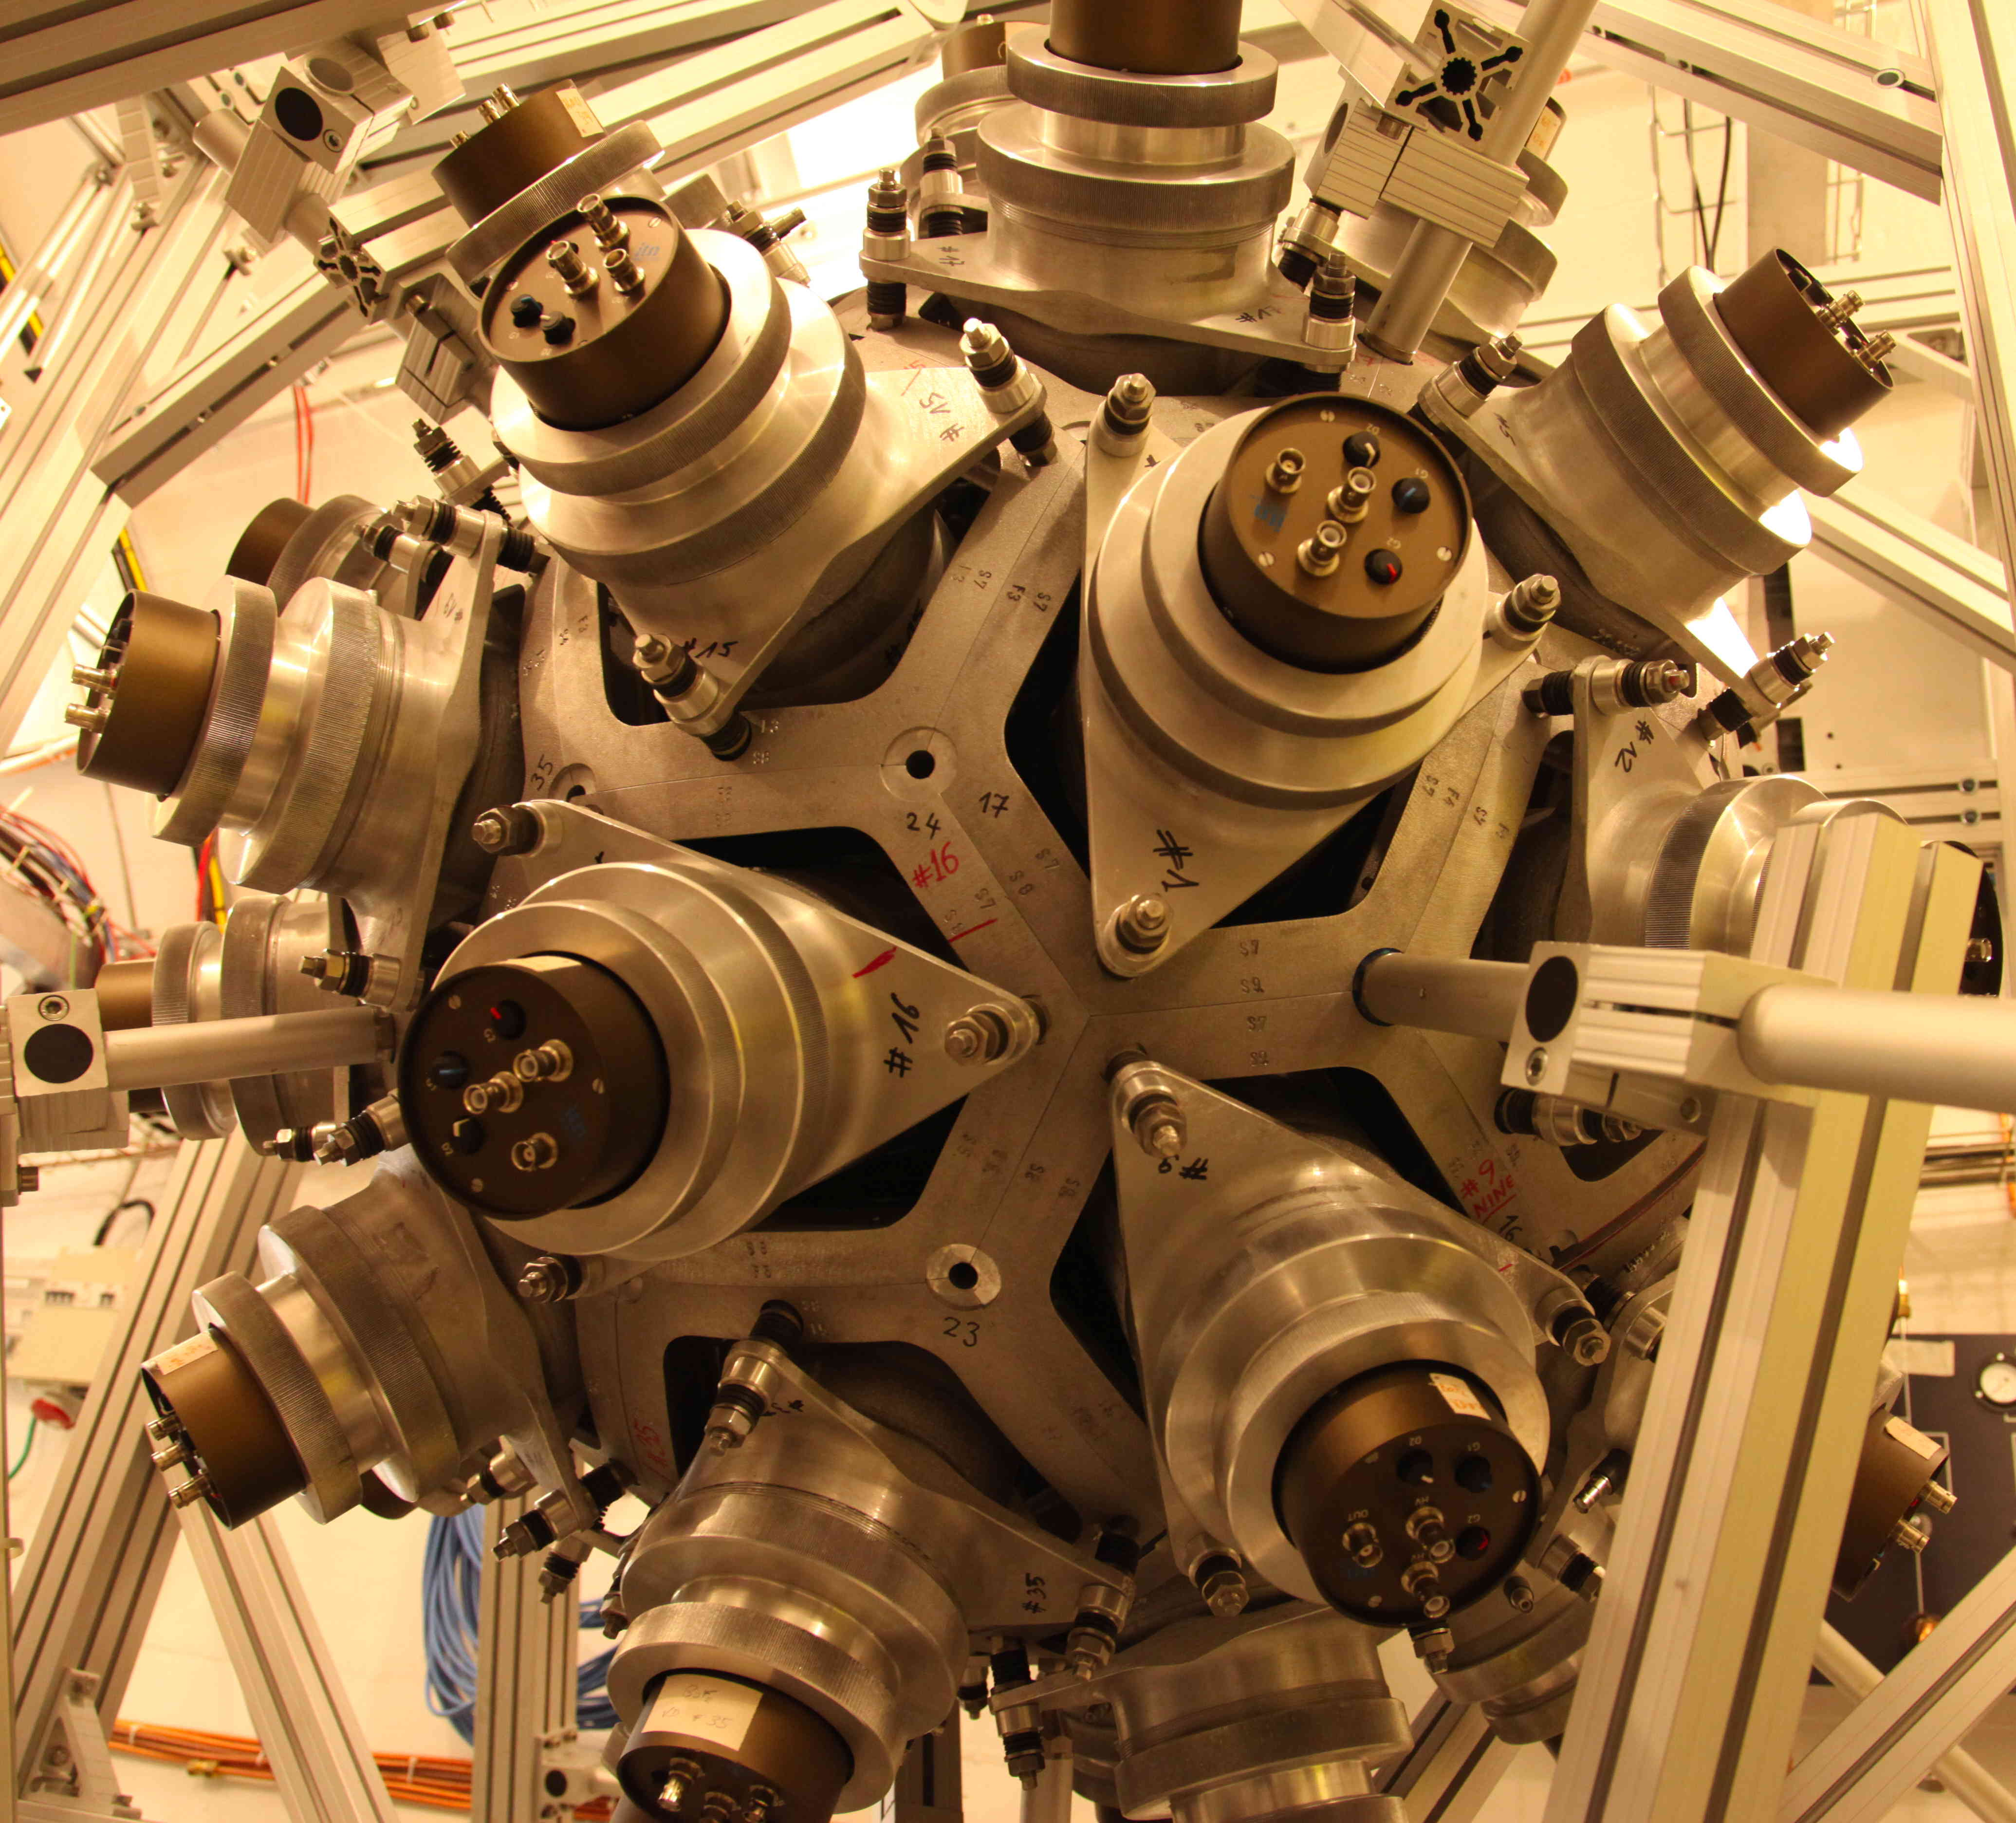
\includegraphics[width=0.9\textwidth]{01_introduction/pics/ntof}
\caption{The calorimeter in the n-ToF area \cite{Maximilien:1304589}.}
\label{fig:ntof}
\end{figure}


% ---------------------------------------------------------------------------------------------------------------
\section{Particle detectors}
Particle detectors, or radiation detectors, have first come into use at the end of the 19th century. At that time Wilhelm R\"ontgen used a photographic plate onto which he shone X-rays. Soon after, in 1912, Victor F. Hess discovered cosmic rays during a balloon flight. This paved the way for development of particle detectors. A cloud chamber was designed -- a chamber filled with a supersaturated vapour of water or alcohol. If a highly energetic particle traversed the chamber, the mixture ionised, creating condensation nuclei. These traces were visible and were photographed. All the subsequent particle detectors relied on the same principle of interaction between the particles -- ionisation. The bubble chamber invented in 1952 used a superheated transparent liquid -- a liquid heated just below its boiling point. A particle ionised the liquid, forming microscopic bubbles along its trajectory. Then followed the spark chamber and the wire chamber where the particle ionised the gas, causing a spark between two parallel plates at a high potential difference. These are nowadays used in museums as showcases. Next were ionisation chambers, which measured the induced current of the free ionised charges moving in an externally applied electric field. Finally in the 1960s, semiconductor detectors were introduced. Their principle of operation is similar to that of an ionisation chamber, with the difference that a semi-conductive material is used as an ionisation medium instead of gas. Nowadays an ensemble of several types of detectors is used as a single detector system. Many considerations need to be taken into account when designing such a system: detector geometry, segmentation, event rate, efficiency, readout, support structures, cabling, cooling, cost etc.

Particle detectors can be divided in two groups: tracking detectors and calorimeters. The former are designed to measure trajectories (momentum) of particles and photons with a minimal impact on their flight path or energy with the aim to optimise the spatial resolution. Typically they are semiconductor detectors. The calorimeters, on the other hand, measure the energy of the particles/photons by stopping them. This means they need to be heavy and dense. A typical physics experiment nowadays would consist of a tracking detector enclosed by a calorimeter. This way both the momentum and energy are derived, measuring energy, charge and trajectory of every particle/photon.

%History and use (1 pg)
%Comparison table (2 pg)

%\subsection{Semiconductor sensors}

\subsection{Semiconductor detectors}
Semiconductor particle detectors are devices that use a semiconductor for detecting radiation. They work on the principle of an ionisation chamber. An incident particle or a photon ionises the atoms in the crystal lattice. The charges are freed if the deposited energy is higher than the energy band gap. The freed charge carriers start drifting in an externally applied electric field, inducing current on the electrodes. 

A number of semiconductor materials exist, each with a different band gap. Germanium (Ge) for instance has a band gap of 0.67~eV, which means that most of the electrons at the room temperature are already in an excited state due to thermal excitation. The 5.5~eV band gap in the diamond, on the other hand, prevents the thermally excited electrons to jump to the conduction band. In addition, the gap is too wide for the visible light to excite the electrons. Silicon with an energy gap of 1.12~eV fulfils most of the needs for particle physics requirements and is therefore the most widely used material for particle detection. 
\begin{figure}[!t]
\centering
\includegraphics[width=0.9\textwidth]{01_introduction/pics/ibl}
\caption{The Insertable B-Layer -- a silicon particle tracker installed in the ATLAS experiment in 2014 \cite{MarcelloniDeOliveira:1702006}.}
\label{fig:ibl}
\end{figure}

Semiconductor detectors are most widely used for tracking applications, like the Insertable B-Layer shown in figure~\ref{fig:ibl}~\cite{Pernegger:1985432}, which was installed in ATLAS Experiment in 2014. First , they can be produced in thin layers to minimise the impact on the path of the incident particles. Second, their low sensor capacitance allows for a fast signal response. Third, they are highly efficient and highly resistant to radiation damage. Finally, the industrial processes allow for a fine spatial segmentation, which in turn improves the track resolution of a detector system. 

Semiconductor sensors come in several configurations. The simplest type is a pad -- a single plate with two electrodes. Pads are used for particle counting and radiation monitoring. Next is a strip detector, a more finely segmented detector made out of long parallel sensing areas or strips. Normally each strip has its own signal line for readout. Usually the strip detectors are used in pairs -- one detector is placed on top of the other at an angle to increase spatial resolution in both axes. The third and the most finely segmented is a pixel detector, consisting of a 2D array of independent sensing areas. In tracking applications, pixel detectors are used where the need for a high detection resolution and granularity is the highest. Due to their high production cost and a high number of signal channels, they can only cover limited areas. Strip detectors are cheaper to produce and can be used to cover larger areas in several consecutive layers.

\subsection{Diamond sensors}
Diamond has been known for over two millennia, valued for its mechanical properties and its appearance. When the procedures for its synthesis were discovered, diamond made its way to a broad range of industries which exploit its optical and electrical properties. The discovery of the Chemical Vapour Deposition (described below) as a new synthesis process gave rise to a range of new applications. Purer specimens are used in electronics, high-power switching devices, electrochemical systems, radiation sensors, quantum computing etc. Recently it was found that it also exhibits superconductivity. This thesis focuses on the use of diamond for radiation detection.
\begin{figure}[!t]
\centering
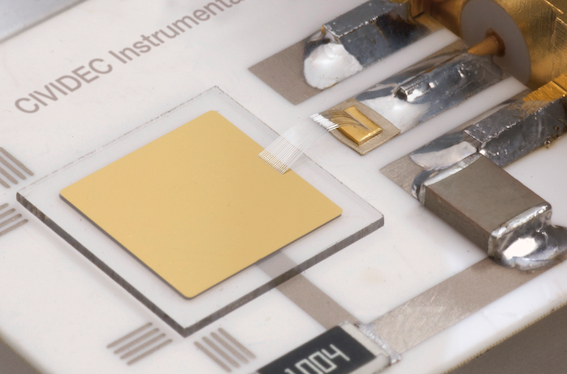
\includegraphics[width=0.9\textwidth]{01_introduction/pics/cividecpcvd}
\caption{A pCVD diamond pad detector \cite{Cividec:00000}.}
\label{fig:cividecpcvd}
\end{figure}

Compared to a natural diamond, a detector-grade CVD diamond has almost no impurities (foreign atoms like nitrogen or boron). If proper procedures are followed, the diamond lattice can be grown very uniformly. This in turn improves electrical properties of the grown sample. Diamond is an almost perfect thermal and electrical insulator. Compared to silicon, the most widely used semiconductor material for radiation detection, it has many advantages, which are described in detail in chapter~\ref{ch:diamond}. Figure~\ref{fig:cividecpcvd} shows a diamond pad sensor produced by CIVIDEC Instrumentation GmbH.
%Its energy band gap is three times as large, reducing the noise and  

\begin{description}
\item[Chemical vapour deposition] (CVD)~\cite{} is a process where a material is deposited from a gas onto a substrate, involving chemical reactions. It is often carried out under high pressure and high temperatures. It takes place in enclosed chambers called furnaces with careful regulation of the temperature, pressure and gas mixture. Synthetic diamond is grown at 700--900 \textdegree C with a mixture of hydrogen and methane gas. At this temperature the molecules dissociate into carbon and hydrogen atoms. The carbon atoms are the building blocks and are deposited on the surface of the substrate.

Under a carefully controlled pressure and temperature conditions with an added abrasive atomic hydrogen the graphitic bonds break and form into diamond bonds. The speed of the growth can be anywhere between 0.1 and 10~$\upmu$m per hour. The detector grade samples are grown at a rate of the order of 1~$\upmu$m per hour. They can grow up to several millimetres in thickness. The width of the samples, however, depends entirely on the substrate used. Diamond can be deposited on various materials: diamond, silicon, tungsten, quartz glass etc. The substrate material must be able to withstand the high temperatures during the CVD process. The diamond substrate does not need any surface pre-treatment. Carbon atoms form bonds with atoms in the existing crystal structure. This is the homo-epitaxial growth where the newly deposited atoms retain the orientation of the structure in the substrate. Other non-diamond substrates, however, need to be pre-treated, usually by being polished using diamond powder. Some powder particles remain on the surface, acting as seeds for the growth of small crystals or grains. These grains grow and at some point merge with the adjacent ones, making up a compact material. The lower side is later polished away. These diamonds are called \emph{polycrystalline} (pCVD) whereas those grown on a diamond substrate are \emph{single crystal} (sCVD) diamonds. The area of the former can be large - up to 0.5~m$^2$ or more compact 15~cm$^2$ in the case of detector grade diamonds. The sCVD diamonds, on the other hand, can currently only measure up to 1.5~cm$^2$.
\end{description}



\chapter{Signal formation in diamond}
\label{ch:diamond}

This chapter describes the fundamentals of signal formation in a diamond sensor, as well as its use as a particle detector. This is described in section~\ref{sec:princsigfor} where the principles of energy deposition are explained. Then the current signal shapes of different types of radiation are shown. Later on the internal lattice defects that affect the signal are described. The final section contains the description of the remaining part of the signal chain -- signal amplifiers, digitisers and devices for signal processing. Noise contributions are discussed at every stage of the signal chain.

Ionisation is the main signal generation mechanism in diamond, silicon and other semiconducting materials. A semiconductor sensor converts the energy deposited by an incident energetic particle to an electrical signal. In particular, the particle ionises the atoms in the lattice, freeing electrons and holes, which then drift towards positively and negatively charged electrodes due to an externally applied electrical field, inducing an electrical signal on the electrodes. 

Silicon is currently considered as the industry standard for particle detection. However, there are several disadvantages of using silicon instead of diamond, due to significant differences in the material properties. In particular, the properties of silicon change significantly with radiation. Due to radiation-induced lattice defects, which act as charge traps, the charge collection efficiency is decreased. The defects are also responsible for the increase of the leakage current, increasing the shot noise eventually leading to a thermal runaway. The same is true for diamond, but on a smaller scale.

Table~\ref{tab:semicompare} compares the properties of diamond and silicon. Some of these values are revisited and used in the course of this thesis. 

\begin{footnotesize}
\begin{center}
\begin{tabular}{   l  c  c   }
\hline
Property & Diamond & Silicon \\
\hline
Band gap energy E$_\mathrm{g}$ (eV) & 5.5 & 1.12  \\
Electron mobility $\upmu_\mathrm{e}$ (cm$^2$ V$^{-1}$ s$^{-1}$) & 1800 & 1350 \\
Hole mobility $\upmu_\mathrm{h}$ (cm$^2$ V$^{-1}$ s$^{-1}$) & 1200 & 450 \\
Breakdown field (V cm$^{-1}$) & $10^{7}$ & $3\times 10^5$ \\
Resistivity ($\Upomega$ cm) & $>10^{11}$  & $2.3\times 10^5$  \\
Intrinsic carrier density (cm$^{-1}$) & $<10^3$ & $1.5\times 10^{10} $ \\
Mass density (g cm$^{-1}$) & $ 3.52$ & $2.33 $ \\
Atomic charge  & $6 $ & $ 14$ \\
Dielectric constant $\upvarepsilon$ & $5.7 $ & $11.9 $ \\
Displacement energy (eV/atom) & $43 $ & $13-20 $ \\
Energy to create an e-h pair  (eV) & $13 $ & $ 3.6$ \\
Radiation length (cm) & $ 12.2$ & $9.6 $ \\
Avg. signal created/$\upmu$m (e) & 36 & 89 \\\hline
\end{tabular}
\captionof{table}{Comparison diamond -- silicon~\cite{ ,Jansen:1956431}.}
\label{tab:semicompare}
\end{center}
\end{footnotesize}


% ---------------------------------------------------------------------------------------------------------------
%\clearpage
\section{Principles of signal formation in semiconductors}
\label{sec:princsigfor}
% ---------------------------------------------------------------------------------------------------------------
%Lattice, electron-hole pair production (3 pg)
%Ramo theorem (2 pg)
%SC detector systems, pg. 43-73
Particles can interact with the sensor in several ways, e.g. via bremsstrahlung~\cite{}, elastic or inelastic scattering (e-h pair production) or nuclear reactions. Bremsstrahlung is radiation created when a particle is decelerated due to interaction with the electric field of the core of an atom. Elastic scattering is deflection of the particle's trajectory due to the pull from the nucleus without depositing any energy in it. This is in principle an unwanted effect in semiconductors as it deteriorates the spatial resolution of the sensor. Inelastic scattering is the interaction through which an atom is ionised and an electron-hole pair is created. All these effects are competing and are dependent on the particle's mass, momentum etc. 

Semiconductors are materials with a conductance between that of insulators and that of metals -- of the order of  $10^{?5}~\Upomega^{-1}$~cm$^{?1}$. They can be made up of atoms with four electrons in their valence band (e.g. silicon--Si, carbon--C or germanium--Ge) or as combinations of two or more different materials (e.g. gallium arsenide--GaAs). The atoms in the lattice form valence bonds with adjacent atoms, making solid crystal structures. 

The valence bonds between atoms in the crystal lattice can break apart if sufficient external energy is deposited. The electron that was forming the bond is excited into the conductance band, leaving behind a positively charged ion with a vacancy -- a hole -- in its valence band, as shown in figure~\ref{fig:semilattice9}. A free electron-hole pair is thus created. The free electron travels through the crystal until it is recombined with another hole. Similarly, the hole also travels through the material. Its positive charge attracts a bound electron in the vicinity, which breaks from the current bond and moves to the vacancy, leaving a new hole behind. The process continues, making it look like the hole is traveling through the material~\cite{}.

%\begin{figure}[!t]
%\begin{center}
%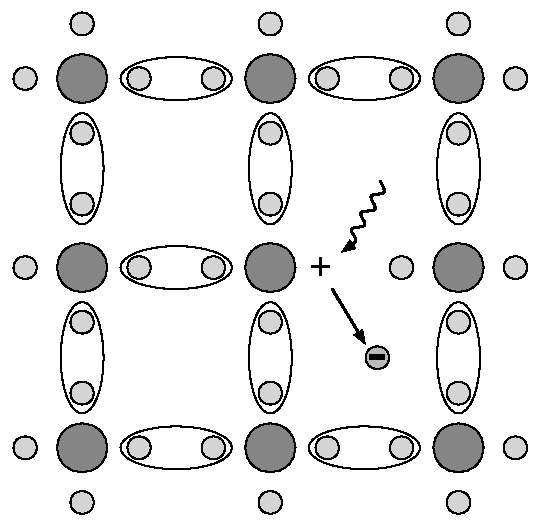
\includegraphics[width=0.4\linewidth]{02_pulse_formation/pics/plots/semilattice9}
%\caption{Valence bonds in the crystalline structure can be broken, producing a free electron-hole pair}
%\label{fig:semilattice9}
%\end{center}
%\end{figure}



The electrons need to absorb a certain energy to get to get ionised. The minimal transferred energy required to excite an electron in a semiconductor is equal to the energy gap $E_\mathrm{g}$. Typical widths of the forbidden gap are 0.7~eV in Ge, 1.12~eV in Si, 1.4~eV in GaAs and 5.5~eV in diamond. Due to the small band gap in semiconductors a significant amount of electrons already occupies the conduction band at room temperature (RT) due to thermal excitation, according to the probabilistic distribution. The intrinsic carrier concentration $n_\mathrm{i}$ in semiconductors is given as
\begin{equation}
\label{eq:intrinsiccarrier}
n_\mathrm{i} = T^{3/2} \cdot \exp\left(-\frac{E_\mathrm{g}}{2k_\mathrm{B}T}\right)
\end{equation} 
wherein $k_\mathrm{B} = 1.381\times10^{-23}~$m$^2~$kg~s$^{-2}~$K$^{-1}$ is the Boltzmann constant, $E_\mathrm{g}$ is the energy band gap of the semiconductor and $T$ is the temperature in K. 
%CONTINEUE 

If an external electric field is applied to the crystalline structure, the free electrons and holes drift toward the positive and negative potential, respectively, as shown in figure~\ref{fig:simpledrift}. While drifting, the charges couple with the electrodes, inducing current in the circuit, which is explained by the Shockley--Ramo theorem below. Upon reaching the electrodes the charges stop inducing the current. The equivalent electrical circuit is shown in figure~\ref{fig:simpledrifteq}.

\begin{figure}[!t]
\begin{tabular}{cccc}
\subfloat[Valence bonds in the crystalline structure can be broken, creating a free electron-hole pair]{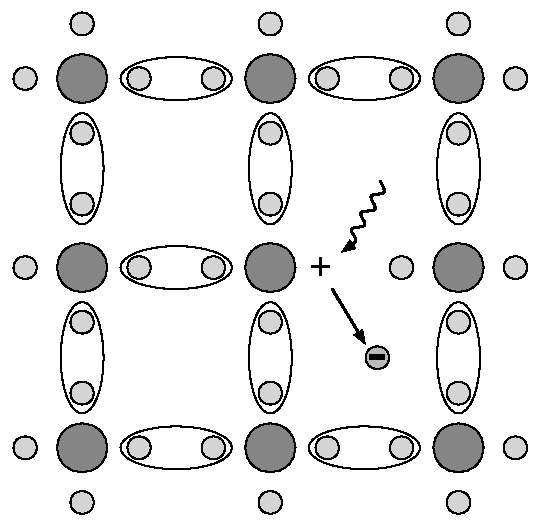
\includegraphics[width=0.22\textwidth]{02_pulse_formation/pics/plots/semilattice9} \label{fig:semilattice9}} &
\subfloat[The freed electron-hole pair starts drifting in the externally applied electric field. The electron and the hole both drift in the opposite directions towards the oppositely charged electrods.]{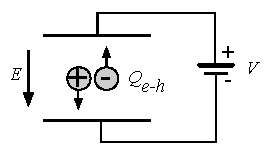
\includegraphics[width=0.32\textwidth]{02_pulse_formation/pics/plots/simpledrift} \label{fig:simpledrift}} &
\subfloat[Equivalent electrical circuit. The moving charges act as a current source.]{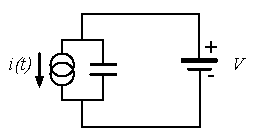
\includegraphics[width=0.34\textwidth]{02_pulse_formation/pics/plots/simpledrifteq}  \label{fig:simpledrifteq}}
\end{tabular}
\caption{In the equivalent electrical circuit diagram the electron-hole creation and drift can be modelled as a current source with a capacitor in parallel.}
\end{figure}



%BETHE-BLOCH
\begin{description}
\item[Mean energy loss] of a particle traversing the detector as a function of the momentum is given with the the Bethe-Bloch equation~\cite{}: 
\begin{equation}
-\left\langle\frac{\mathrm{d}E}{\mathrm{d}x}\right\rangle = \frac{4\pi}{m_\mathrm{e}c^2}  \cdot \frac{nz^2}{\beta^2}  \cdot  \left(\frac{e^2}{4\pi\epsilon_\mathrm{0}}\right)^2  \cdot  \left( \ln \left(\frac{2m_\mathrm{e}c^2\beta^2}{I\cdot(1-\beta^2)}\right)-\beta^2  \right)
\label{eq:bethebloch}
\end{equation}
The resulting function for a muon is shown in figure~\ref{fig:bb2}. At a momentum of around 300~MeV/c the particle deposits the lowest amount of energy. That is called a minimum ionising particle or a MIP.
\end{description}


\begin{figure}[!t]
\begin{center}
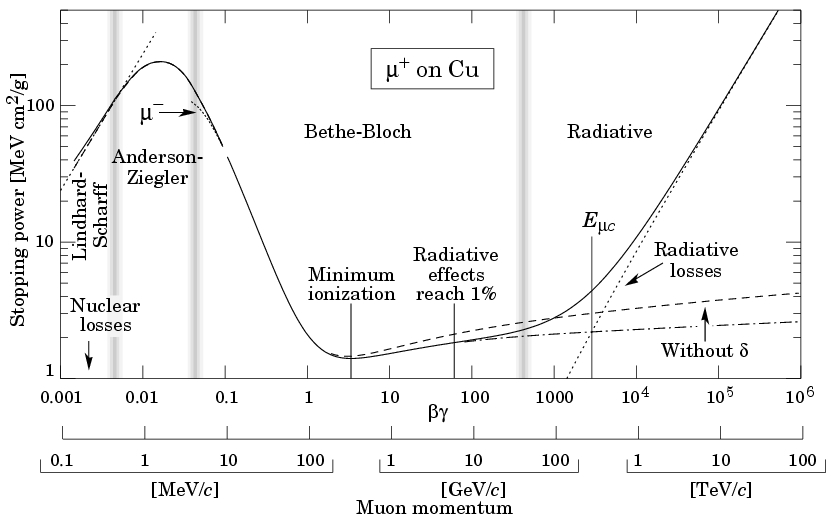
\includegraphics[width=0.85\linewidth]{02_pulse_formation/pics/bb2}
\caption{Stopping power for muons according to the Bethe-Bloch formula~\cite{}.}
\label{fig:bb2}
\end{center}
\end{figure}


\subsection{Signal induction by moving charges}
The signal induction in a conducting plane by a point-like charge, which couples with an electrode, is derived in~\cite{PDDC:00000}. The electrode can in this case be modelled as an infinite conducting plane. When a point charge $q$ is created (e.g. an electron-hole pair created via ionisation), its electrostatic field lines immediately couple with the electrode, as seen in figure~\ref{fig:chargeind1}. The electric field on the metal surface due to a point-like charge $q$ at the distance $z_\mathrm{0}$ is
\begin{equation}
E_\mathrm{z}(x,y) = \frac{qz_\mathrm{0}}{2\pi\epsilon_\mathrm{0}(x^2+y^2+z_0^2)^\frac{3}{2}}~~~~~~~~~~E_\mathrm{y} = E_\mathrm{z} = 0.
\end{equation}
\begin{figure}[!t]
%\centering
\begin{tabular}{cccc}
\subfloat[Newly created point charge couples with the conductive plane.]{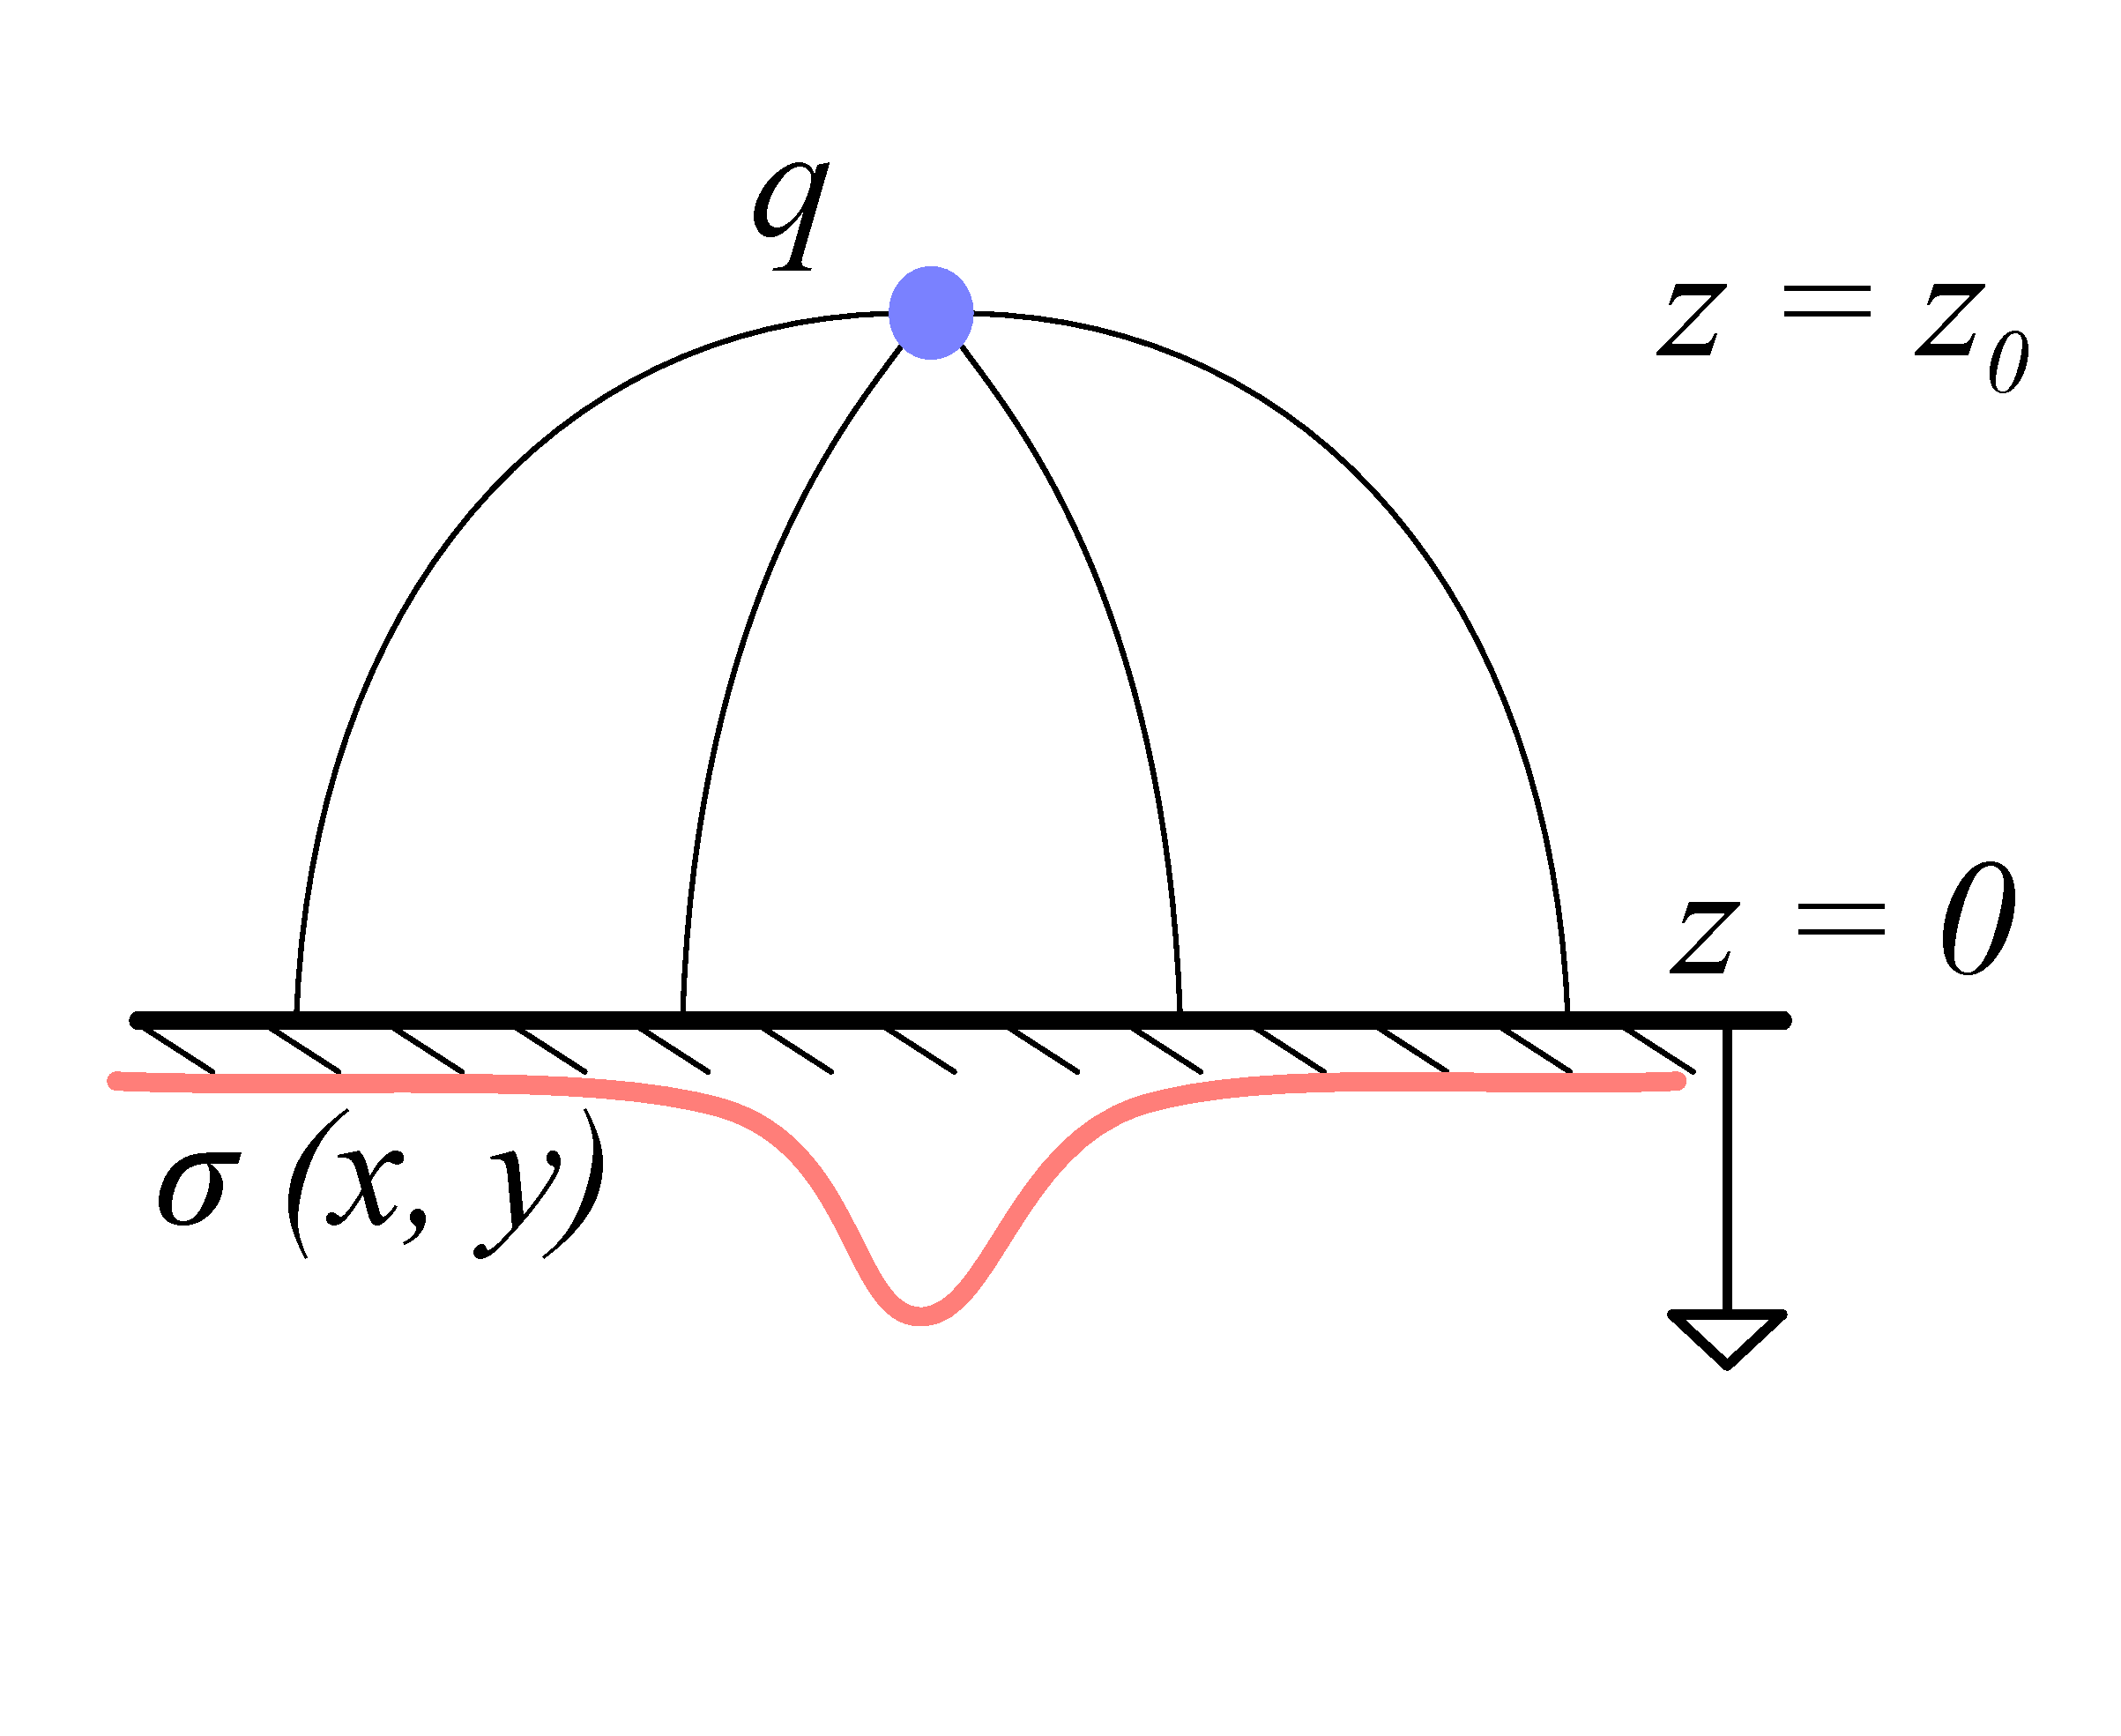
\includegraphics[width=0.30\textwidth]{02_pulse_formation/pics/plots/chargeind1} \label{fig:chargeind1}} &
\subfloat[When the charge drifts, the charge density in the plane changes.]{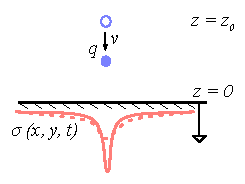
\includegraphics[width=0.30\textwidth]{02_pulse_formation/pics/plots/chargeind2} \label{fig:chargeind2}} &
\subfloat[The changing charge density in the small regions of the plane induces current.]{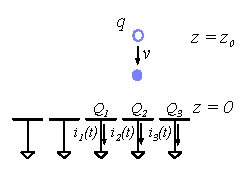
\includegraphics[width=0.30\textwidth]{02_pulse_formation/pics/plots/chargeind3}  \label{fig:chargeind3}}
\end{tabular}
\caption{A point-like charge inducing current in a conductive plane.}
\end{figure}
A mirror charge appears on the conducting plane, with a charge density distribution
\begin{equation}
\label{eq:chgdnstydist}
\sigma(x,y)=\epsilon_\mathrm{0}E_\mathrm{z}(x,y)=\frac{qz_\mathrm{0}}{2\pi(x^2+y^2+z_0^2)^\frac{3}{2}}.
\end{equation}
The charge density integrated over the entire plane yields a mirror charge $Q$, which is an opposite of point charge $q$:
\begin{equation}
\label{eq:chargedensity}
Q=\int_{-\infty}^{\infty} \int_{-\infty}^{\infty} \sigma(x,y)\mathrm{d}x\mathrm{d}y = -q.
\end{equation}
The plane is then segmented into infinitely long strips with a width $w$ whereby each of the strips is grounded, as shown in figure~\ref{fig:chargeind3}. Considering a charge density distribution~\ref{eq:chgdnstydist}, the resulting mirror charge on a single strip $Q_\mathrm{2}$ directly below the point charge $(x=0, y=0)$ yields
\begin{equation}
\label{eq:stripcharge}
Q_\mathrm{2}(z_\mathrm{0})=\int_{-\infty}^{\infty}\int_{-w/2}^{w/2}\sigma(x,y)\mathrm{d}x\mathrm{d}y = -\frac{2q}{\pi}\arctan\left(\frac{w}{2z_\mathrm{0}}\right)
\end{equation} 
If the charge starts moving towards the conducting plane, the mirror charge density distribution also changes, as shown in figure~\ref{fig:chargeind2}. As a result the $Q_2[z(t)]$ changes with time. The changing charge is in effect an induced electric current $i_2(t)$:
 \begin{equation}
 \label{eq:indcurr}
 i_2(t) = -\frac{\mathrm{d}}{\mathrm{d}t}Q_\mathrm{2}[z(t)] = -\frac{\partial Q_\mathrm{2}[z(t)]}{\partial z}\frac{\partial z(t)}{\partial t} = \frac{4qw}{\pi[4z(t)^2 + w^2]}v. 
 \end{equation}
 The movement of the point-like charge therefore induces current in the conducting plane. The induced current is linearly dependent on the velocity of the point-like charge.

\subsection{Shockley-Ramo theorem}
W. Shockley~\cite{SHOCKLEY:00000} and S. Ramo~\cite{RAMO:00000} independently proposed a theory which explains how a moving point charge induces current in a conductor. The Shockley-Ramo theorem can therefore be used to calculate the instantaneous electric current induced by the charge carrier or a group of charge carriers. It can be used for any number of electrodes. It states that the current $I_\mathrm{n}^{\mathrm{ind}}(t)$ induced on the grounded electrode $n$ by a point charge $q$ moving along a trajectory $\textbf{x}(t)$ reads
\begin{equation}
\label{eq:ramo}
I_\mathrm{n}^{\mathrm{ind}}(t) = -\frac{\mathrm{d}Q_\mathrm{n}(t)}{\mathrm{d}t} =  -\frac{q}{V_\mathrm{w}}\nabla\Psi_\mathrm{n}[\textbf{x}(t)]v(t)  =  -\frac{q}{V_\mathrm{w}}\textbf{E}_\mathrm{n}[\textbf{x}(t)]v(t),
\end{equation}
where $\textbf{E}_\mathrm{n}(\textbf{x})$ is the \emph{weighting field} of electrode $n$ in the case where the charge q is removed, electrode $n$ is  set to voltage $V_\mathrm{w}=1$ and all other electrodes are grounded.  The weighting field is defined as the spatial differential of the \emph{weighting potential}: $\textbf{E}_\mathrm{n}(\textbf{x})=\nabla \Psi_\mathrm{n}(\textbf{x})$. In the case of two parallel electrodes, the weighting field is $E_\mathrm{w} = -\frac{\mathrm{d}\Psi}{\mathrm{d}x} = -1/d$, where $d$ is the distance between the electrodes. The resulting induced current is therefore
\begin{equation}
\label{eq:ramoparallel}
i(t) = \frac{q}{d}v_\mathrm{drift}(x,t),
\end{equation} 
whereby $v_{\mathrm{drift}}$ is the drift velocity of the point-like charge and $d$ is the distance between the electrodes. $d$ is defined by the dimensions of the sensor. The drift velocity is a function of the externally applied electric field, as defined in section~\ref{sec:carrtransp}. If the electric field is set to a constant value, the induced current is directly proportional to the drifting charge. Therefore, by measuring the height of the induced current at a specific point of time the number of moving charges can be deduced.


%moving charge->changed i

%shortened derivation

%i=e/vd


%The energy from an incoming particle can be absorbed by lattice excitation (phonon production) or by ionisation (formation of a mobile charge pair). For a single event, the deposited energy E$_{0}$ is equal to the sum of the energies going into excitation (E$_{ex}$) and ionisation (E$_{ion}$)
%\begin{equation}
%\label{eq:excitationionisation}
%E_0 = E_{ex} N_{ex} + E_{ion} N_{ion}
%\end{equation} 
%where N$_{ex}$ is the number of excitations (phonos produced) and N$_Q$ is the number of charge pairs released. For this event, if more 


\subsection{Radiation-induced electrical pulses}

\begin{figure}[!t]
\begin{center}
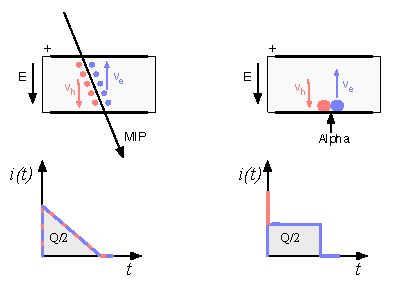
\includegraphics[width=0.8\linewidth]{02_pulse_formation/pics/plots/driftboth}
\caption{Charge carrier drift in diamond for $\upbeta/\upgamma$ and for $\upalpha$ particles crossing the sensor at $t=0$.}
\label{fig:drift}
\end{center}
\end{figure}

When a highly-energetic particle travels through the sensor, it interacts with atoms in the lattice. It ionises the valence electrons, creating electron-hole (e-h) pairs on its way. It can either deposit only a fraction of its energy and exit the sensor on the other side or it can get stopped in the bulk, depositing all of its energy. A special case is when it interacts with the core of the atom in the middle of the sensor via a nuclear interaction. All these various types interactions produce different amounts and different spatial distributions of e-h pairs. The induced electrical current therefore differs for different types of interaction. Two most frequent types are shown in figure~\ref{fig:drift}. The first diagram shows the interaction of a minimum ionising particle. The electrons and holes are created all along the trajectory of the particle and immediately start drifting towards the positive and negative electrode, respectively. At the beginning, all charges drift and contribute to the induced current. Those closest to the electrodes have a very short drift path, reducing the induced current. Gradually all the charge carriers reach the electrode. The resulting current signal is a triangular pulse with a sharp rising edge and a linear falling edge. The accumulated charge $Q_\mathrm{s}$ equals to the sum of the contributions of the positive and negative charge carriers. The second type of interaction happens when the particle is stopped in the diamond close to the point of entry. Most of its energy is deposited in a small volume close to the electrode. A cloud of charge carriers is created and the charges with the shorter path to the electrode disappear almost instantly. The carriers of the opposite charge, however, start drifting through the sensor to the other electrode. In an ideal diamond sensor, their velocity is constant throughout the drift up until they are collected at the opposite electrode. The contribution of the first charge cloud is a peak with a short time. The cloud drifting through the sensor, on the other hand, induces a current signal with a flat top. The resulting signal has a shape of a rectangle, with a spike in the beginning. %This spike is filtered out by a current amplifier in a real device because it is too fast for the electronics existing currently. 
The accumulated charge $Q_\mathrm{s}$ is equal to a half of the deposited charge by the stopped particle.

The two aforementioned types of interactions have well defined signal responses. Nuclear interactions on the other hand yield various results. The resulting signal shape depends on the decay products of the interaction, which can be $\upalpha$, $\upbeta$ or $\upgamma$ quanta or other nuclei, inducing a mixed shaped signal. 
%
%Current profiles
%Alpha
%beta
%gamma
%neutron


\subsection{Signal charge fluctuations}
Two important sensor properties are the magnitude of the signal and the fluctuations of the signal at a given absorbed energy. They determine the relative resolution $\Updelta E/E$. For semiconductors the signal fluctuations are smaller than the simple statistical standard deviation $\upsigma_\mathrm{Q}=\sqrt{N_\mathrm{Q}}$. Here $N_\mathrm{Q}$ is the number of released charge pairs, i.e. the ratio between the total deposited energy $E_\mathrm{0}$ and the average energy deposition $E_\mathrm{i}$ required to produce an electron-hole pair. \cite{} shows that the standard deviation is $\upsigma_\mathrm{Q}=\sqrt{F N_\mathrm{Q}}$, where $F$ is the Fano factor~\cite{} (0.08 for diamond and 0.115 for silicon ~\cite{}). Thus, the standard deviation of the signal charge is smaller than expected, $\upsigma_\mathrm{Q}\approx0.3 \sqrt{N_\mathrm{Q}}$. The resulting intrinsic resolution of semiconductor detectors is 
\begin{equation}
\label{eq:efwhm}
\Updelta E_\mathrm{FWHM} = 2.35 \sqrt{FEE_\mathrm{i}} 
\end{equation} 
wherein $E_\mathrm{i}(Si)$=~3.6~eV and E$_\mathrm{i}(C)$=~13~eV. E.g., for an $\upalpha$ particle with energy $E_\upalpha$ = 5.486 MeV the calculated resolution in diamond is equal to $\Updelta E_{\mathrm{FWHM}}$ = 5.6~keV. This defines the minimum achievable resolution for energy spectroscopy with semiconductors. Figure~\ref{fig:enerres} shows the resolution limit as a function of energy in silicon and diamond.

\begin{figure}[!t]
\begin{center}
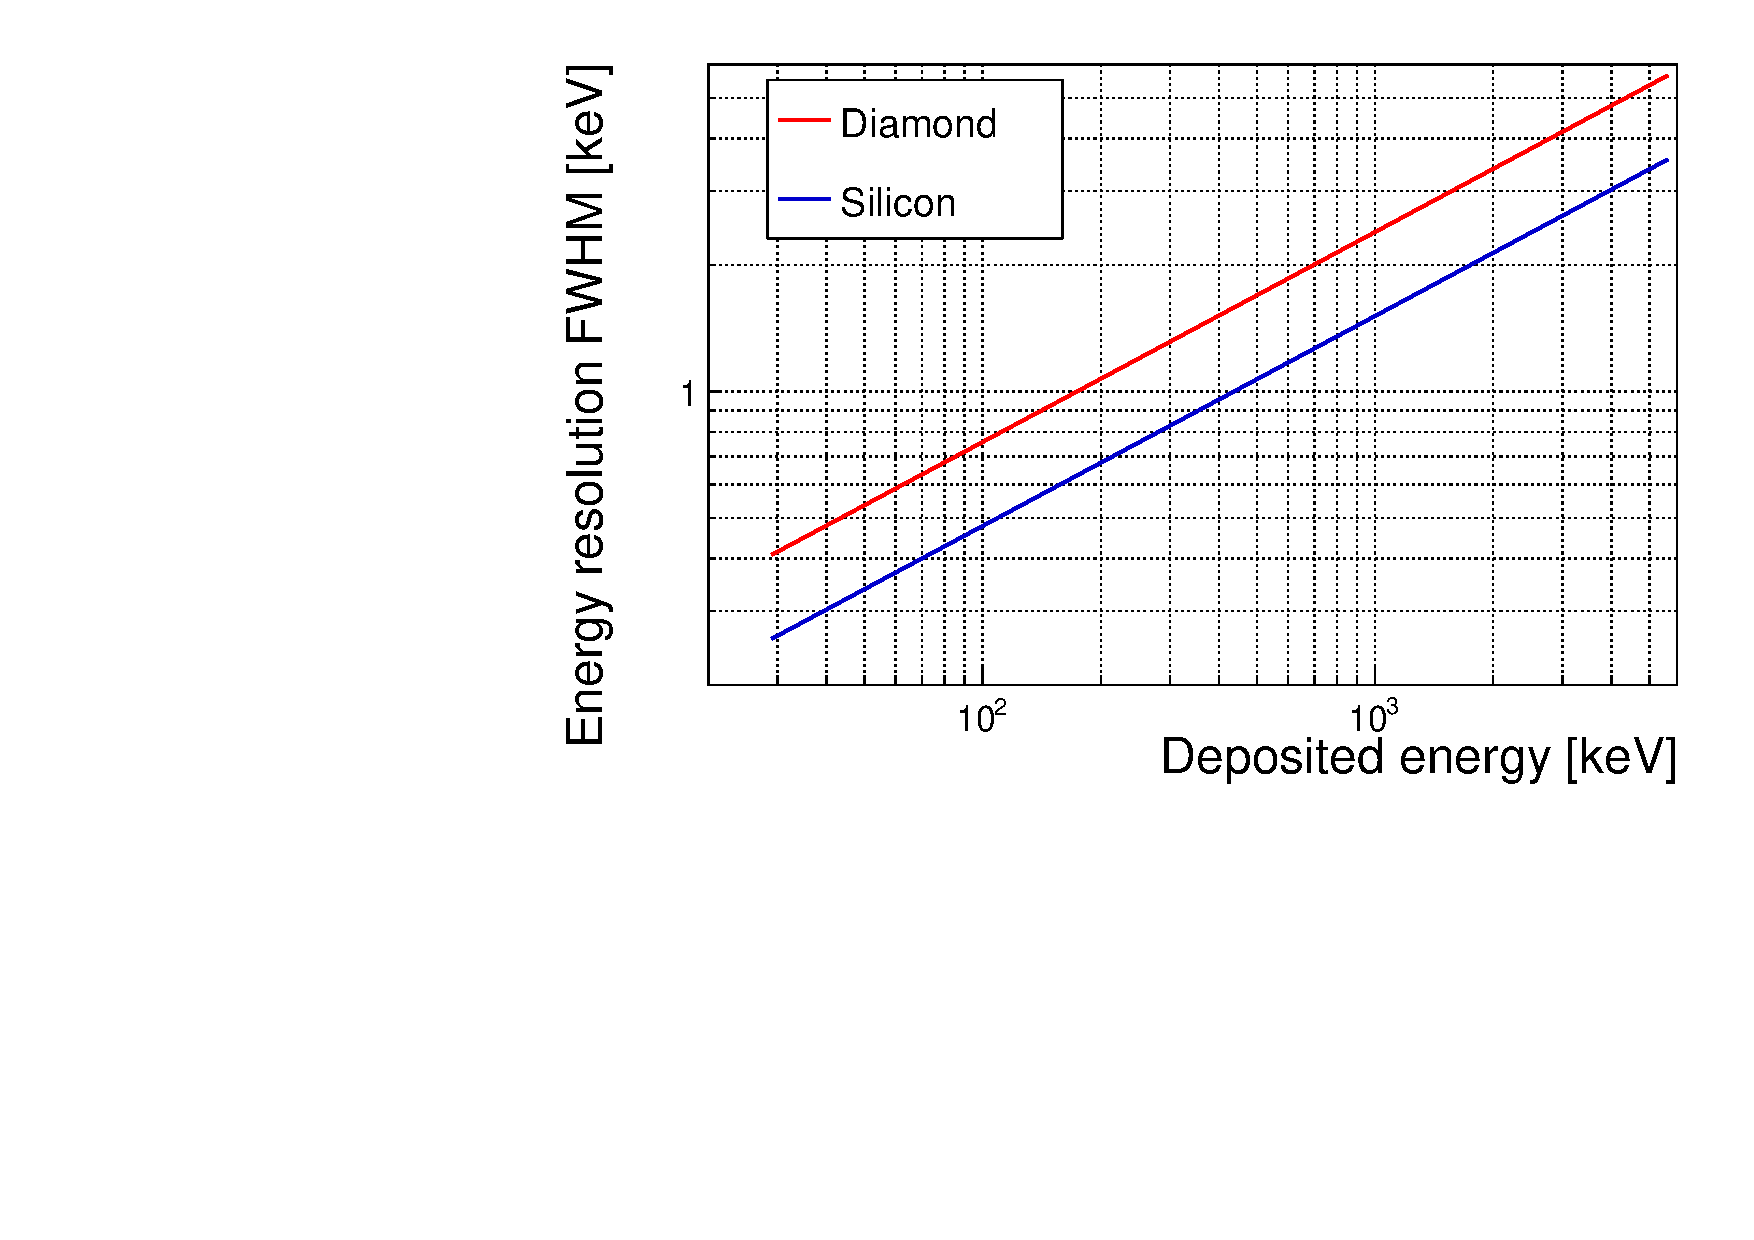
\includegraphics[width=0.8\linewidth]{../scripts/02_pulse_formation/plots/resolution}
\caption{Calculated intrinsic energy resolution for silicon and diamond.}
\label{fig:enerres}
\end{center}
\end{figure}




% ---------------------------------------------------------------------------------------------------------------
%\clearpage
\section{Carrier transport in a diamond sensor} 
\label{sec:carrtransp}
% ---------------------------------------------------------------------------------------------------------------
This section describes the carrier transport phenomena in diamond. This theory provides the basis for discussion about the measurements in chapter~\ref{ch:meas}. 

When the charge carriers are freed in a semiconductor with no concentration gradient and without an externally applied electric field, they scatter in random directions with a thermal velocity $v_{\mathrm{th}}$~\cite{}. Their integral movement due to thermal excitation equals zero. 

\begin{description}

\item[Diffusion]
Diffusion is caused by the concentration gradient. In its presence the integral movement is in the direction of the lower concentration until an equilibrium is reached.
The concentration profile dissolves with time forming a Gaussian distribution with variance $\sigma(t)=\sqrt{Dt}$~\cite{} .

\item[Drift]
Drift is caused by an externally applied electrical field. In that case the carriers move along the field lines. In a sensor with a high applied field the diffusion contribution is negligible. 

\item[Drift velocity, saturation velocity and mobility]
The charge carriers drift through the diamond bulk with a drift velocity $v_\mathrm{drift}(E)$~\cite{}, which is proportional to the electric field $E$ at low electric fields: $v_\mathrm{drift} = \mu E$. The proportionality factor $\mu$ is defined as the mobility in cm$^2$V$^{-1}$s$^{-1}$.

For higher fields and higher velocities, however, the carriers lose more energy to the lattice. They induce increasingly more lattice vibrations (phonon transport). There is a velocity limit above which the carriers cannot reach -- velocity saturation. The $v^e_\mathrm{sat}=v^h_\mathrm{sat}=(14.23\pm0.12)\times10^6$~cm/s for both positive and negative charge carriers has been derived from the measurements in~\cite{JANSEN:00001}.

The final equation for $v_\mathrm{drift}$ is therefore
\begin{equation}
\label{eq:vsat}
v_\mathrm{drift}(E) = \mu(E)E= \frac{\mu_\mathrm{0} E}{1 + \frac{\mu_\mathrm{o} E}{v_\mathrm{sat}}}
\end{equation}
where $\mu_\mathrm{0}$ is the low field mobility and $v_\mathrm{sat}$ is saturation velocity. The drift velocity can be retrieved experimentally via the transit time measured with the Transient Current Technique (TCT). This technique enables the measurement of transit time $t_\mathrm{t}$ of the carriers through the sensor with the thickness $d$. 
\begin{equation}
\label{eq:vsat}
v_\mathrm{drift}(E) = \frac{d}{t_\mathrm{t}(E)}.
\end{equation}
The velocities for holes and electrons usually differ. In diamond, the holes travel 30~\% faster than electrons~\cite{}. The measurements in chapter~\ref{ch:meas} empirically confirm this statement.

\item[Space charge] 
The Poisson equation shows that 
\begin{equation}
\label{eq:poisson}
\frac{d^2\Phi(x)}{\mathrm{d}x^2} = \frac{dE(x)}{\mathrm{d}x} = \frac{\rho(x)}{\epsilon}
\end{equation}
where $\rho(x)$ is the space charge distribution, $E$ is the electrical field and $\Phi$ is the voltage potential. In an ideal diamond, the externally applied high voltage potential on the two electrodes decreases linearly through the bulk. The electrical field is therefore constant throughout the sensor and the space charge distribution across it equals 0. However, space charge may be introduced in the bulk either by means of accumulating of charge carriers in the lattice (i.e. charge trapping) or already during sensor production. The space charge can be either permanent or changing -- sometimes it is possible to reduce it, as is shown in chapter~\ref{ch:meas}. All in all, it is very important to reduce it because it affects the shape of the electrical signal. Since the drift velocity of the charge carriers is proportional to the electrical field, the charges change their velocity while drifting through the space charge region. Figure~\ref{fig:spcchg} compares the voltage potential, the electrical field and the space charge for an ideal sensor as well as for that with a uniformly distributed positive space charge.
\begin{figure}[!t]
\begin{center}
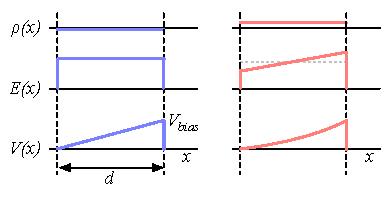
\includegraphics[width=0.6\linewidth]{02_pulse_formation/pics/plots/spcchg}
\caption{Left figure shows a profile of a diamond sensor only with an externally applied electric field. In the figure on the right a uniformly distributed space charge is added in the diamond, contributing to  the internal electric field distribution. The induced current signal is proportional to the electrical field. $d$ is the thickness of the diamond sensor.}
\label{fig:spcchg}
\end{center}
\end{figure}


\item[Radiation damage]
The bonds in the diamond lattice are very strong. However, when highly energetic particles hit the diamond, they can damage the crystal structure. Figure~\ref{fig:raddamage} shows several examples of lattice damage:
\begin{enumerate}
\item[a)]foreign interstitial (e.g. H, Li),
\item[b, c)]foreign substitutional (e.g. N, P, B),
\item[d)]vacancy and
\item[e)]self interstitial.
\end{enumerate} 
These non-uniformities form new energy levels in the forbidden gap -- the separation between the conductive and valence band in which the electrons. These intermediate levels are referred to as charge traps because they can trap moving charge carriers. The energy level of the trapped carriers is reduced from the conduction band to the energy level of the trap. Different types of lattice damage have different energy levels. The carriers trapped in an energy level close to the conduction band have a high probability of being thermally excited back into the conduction band whereby they continue drifting towards the electrode. Their activation energy is therefore low. Those trapped in a deep trap close to the middle of the forbidden gap need a much higher activation energy, which in turn increases the average time to their release due to thermal excitation.

The trapped carriers do not contribute to the overall induced current on the electrodes. The more charges are trapped along their drift path, the lower current is induced on the electrodes.

\begin{figure}[!t]
\begin{center}
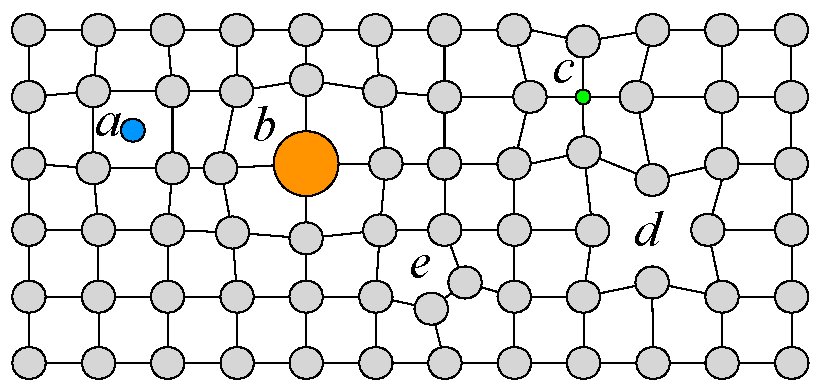
\includegraphics[width=0.8\linewidth]{02_pulse_formation/pics/plots/raddamage}
\caption{Impurities and non-uniformities in the crystal lattice due to radiation damage.}
\label{fig:raddamage}
\end{center}
\end{figure}

\end{description}













% ---------------------------------------------------------------------------------------------------------------
%\clearpage
\section{Electronics for signal processing} % signal acquisition
% ---------------------------------------------------------------------------------------------------------------
\label{sec:elecsigproc}
This section describes the electronics of a detector, starting with a description of signal amplifiers and then discussing the digitisation and signal processing. All these stages are necessary to extract information from the sensor. First, the signal has to be amplified. Then it is digitised and finally processed in a specially designed processor or a logic unit.

\subsection{Signal preamplifiers}
The signal charge generated in the sensor by a single energetic particle is of the order of fC. The induced current range is typically between $10^{-8}$~A ($\upbeta, \upgamma$ radiation) and $3\times10^{-7}$~A ($\upalpha$ radiation). Signals as low as these have to be pre-amplified before processing. Depending on the measurement, several types of signal amplifiers can be used. The preamplifiers are designed to minimise electronic noise while maximising gain, thus maximising the signal-to-noise ratio (SNR). In addition, a high bandwidth limit is preferred to minimise the information loss due to signal shape deformation. A critical parameter is the total capacitance, i.e. the sensor capacitance together with the input capacitance of the preamplifier. The SNR improves with a lower capacitance. Several types of amplifiers can be used, all of which affect the measured pulse shape. Two preamplifiers are used most commonly, a current and a charge sensitive amplifier. Both are described in detail below. 

\begin{figure}[!t]
%\centering
\begin{tabular}{cccc}
\subfloat[A capacitive source and a current amplifier.]{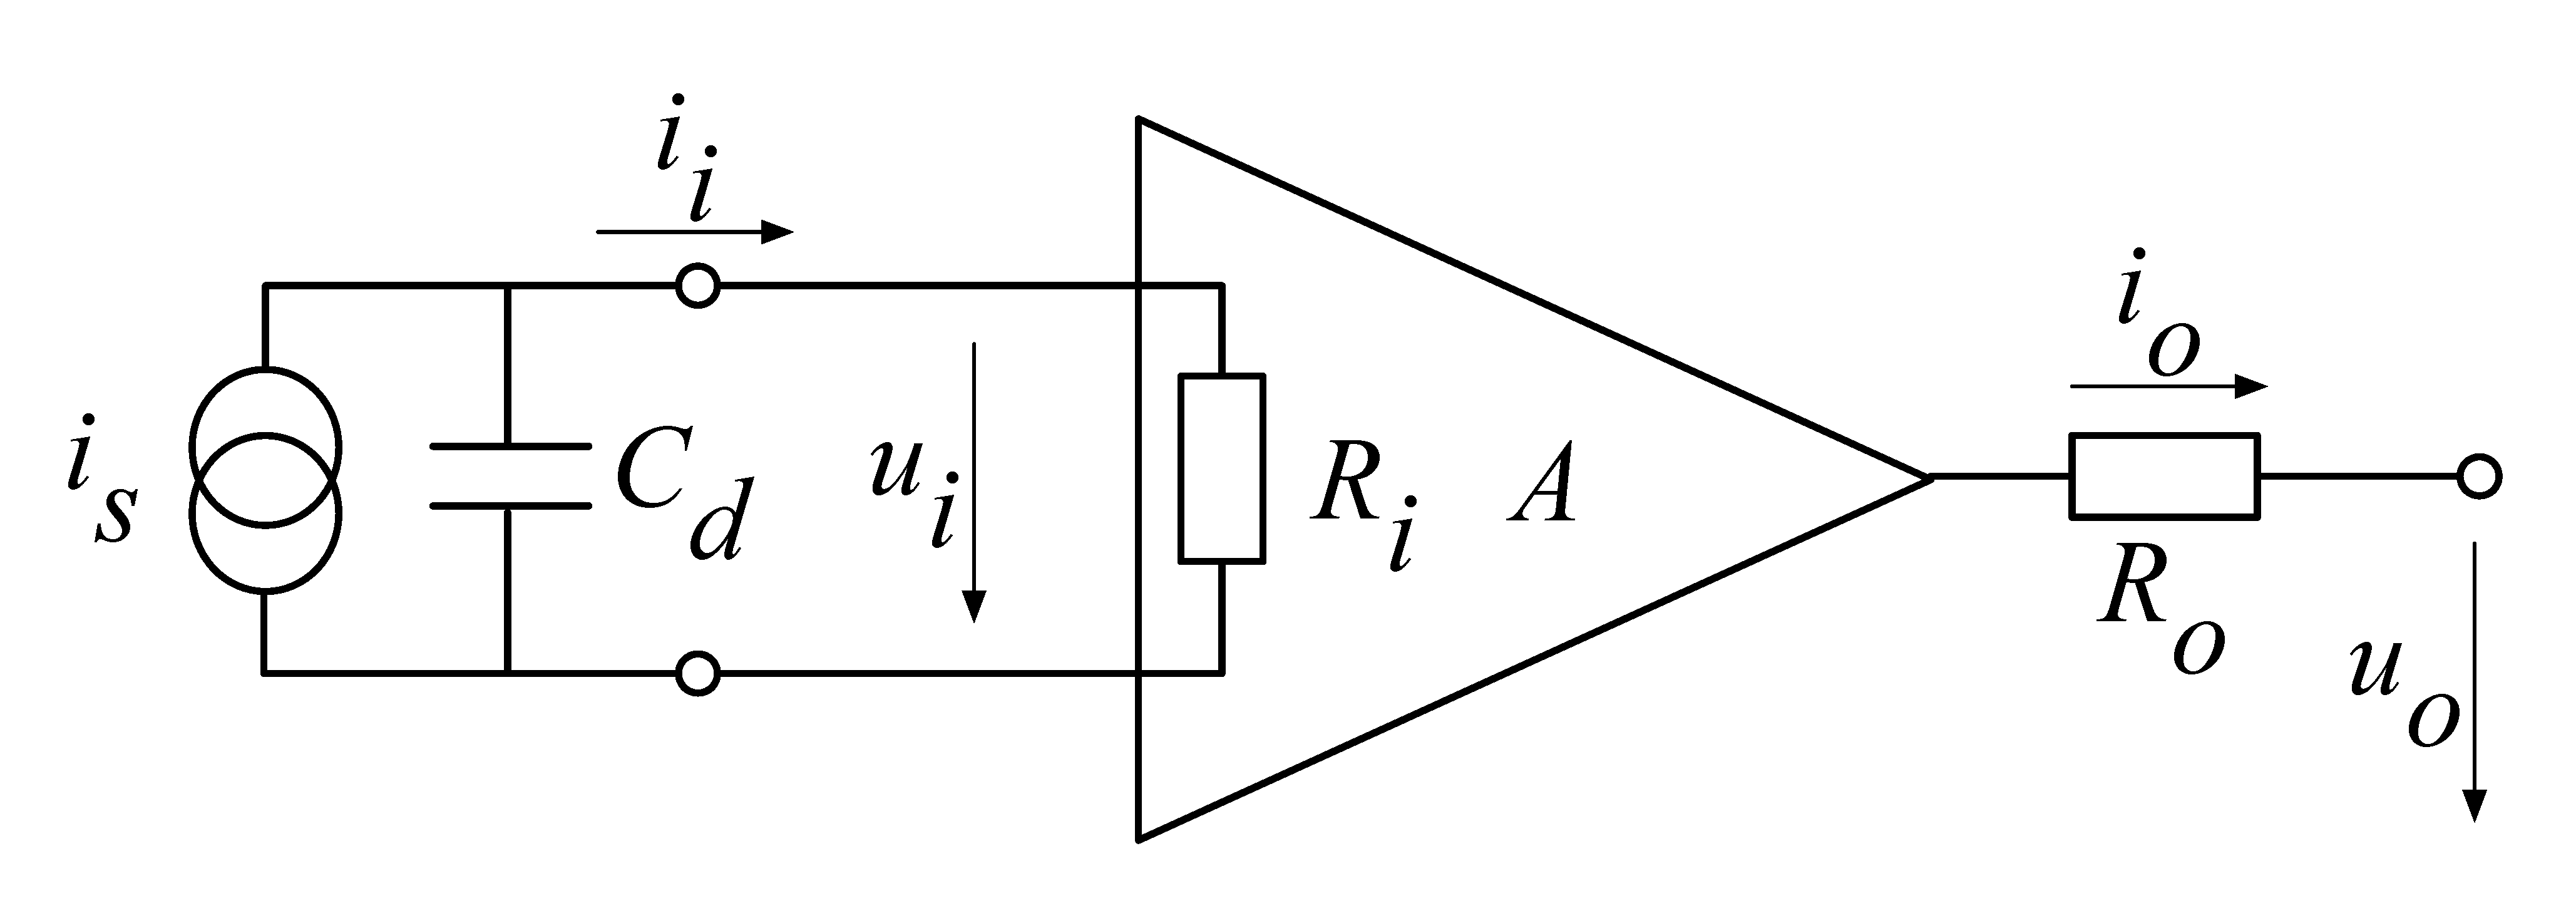
\includegraphics[width=0.50\textwidth]{02_pulse_formation/pics/plots/curramp} \label{fig:curramp}} &
\subfloat[A capacitive source and a charge amplifier.]{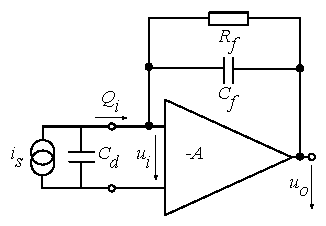
\includegraphics[width=0.40\textwidth]{02_pulse_formation/pics/plots/chgamp}  \label{fig:chgamp}}
\end{tabular}
\caption{Simplified equivalent circuits of a current and charge amplifier.}
\end{figure}


\subsubsection{Current-sensitive amplifier}
Figure~\ref{fig:curramp} shows the equivalent circuit of a capacitive source and a current amplifier. An amplifier operates in current mode if the source has a low charge collection time $t_\mathrm{c}$ with respect to the $R_\mathrm{i}C_\mathrm{d}$ time constant of the circuit. In this case the sensor capacitance discharges rapidly and the output current $i_\mathrm{o}$ is proportional to the instantaneous current $i_\mathrm{i}$. The amplifier is providing a voltage gain, so the output signal voltage $u_o$ is directly proportional to the input voltage $u_\mathrm{i}$:
\begin{equation}
u_\mathrm{o}(t) = A \cdot R_\mathrm{i} \cdot i_\mathrm{s}(t).
\end{equation}
The detector capacitance $C_\mathrm{det}$ together with the input resistance of the amplifier $R_\mathrm{i}$ defines the time constant of the signal, as shown in figure~\ref{fig:currc}. The higher the $C_\mathrm{det}$, the slower is the response of the amplifier. For the case of the diamond sensor, which has the capacitance of the order of 2~pF and the input resistance of 50~$\Omega$, the resulting time constant is $\tau=10^{-10}$~s. This yields the signal rise time $t_\mathrm{r}\sim2.2\tau=2.2\times10^{-10}$~s.
\begin{figure}[!t]
\begin{center}
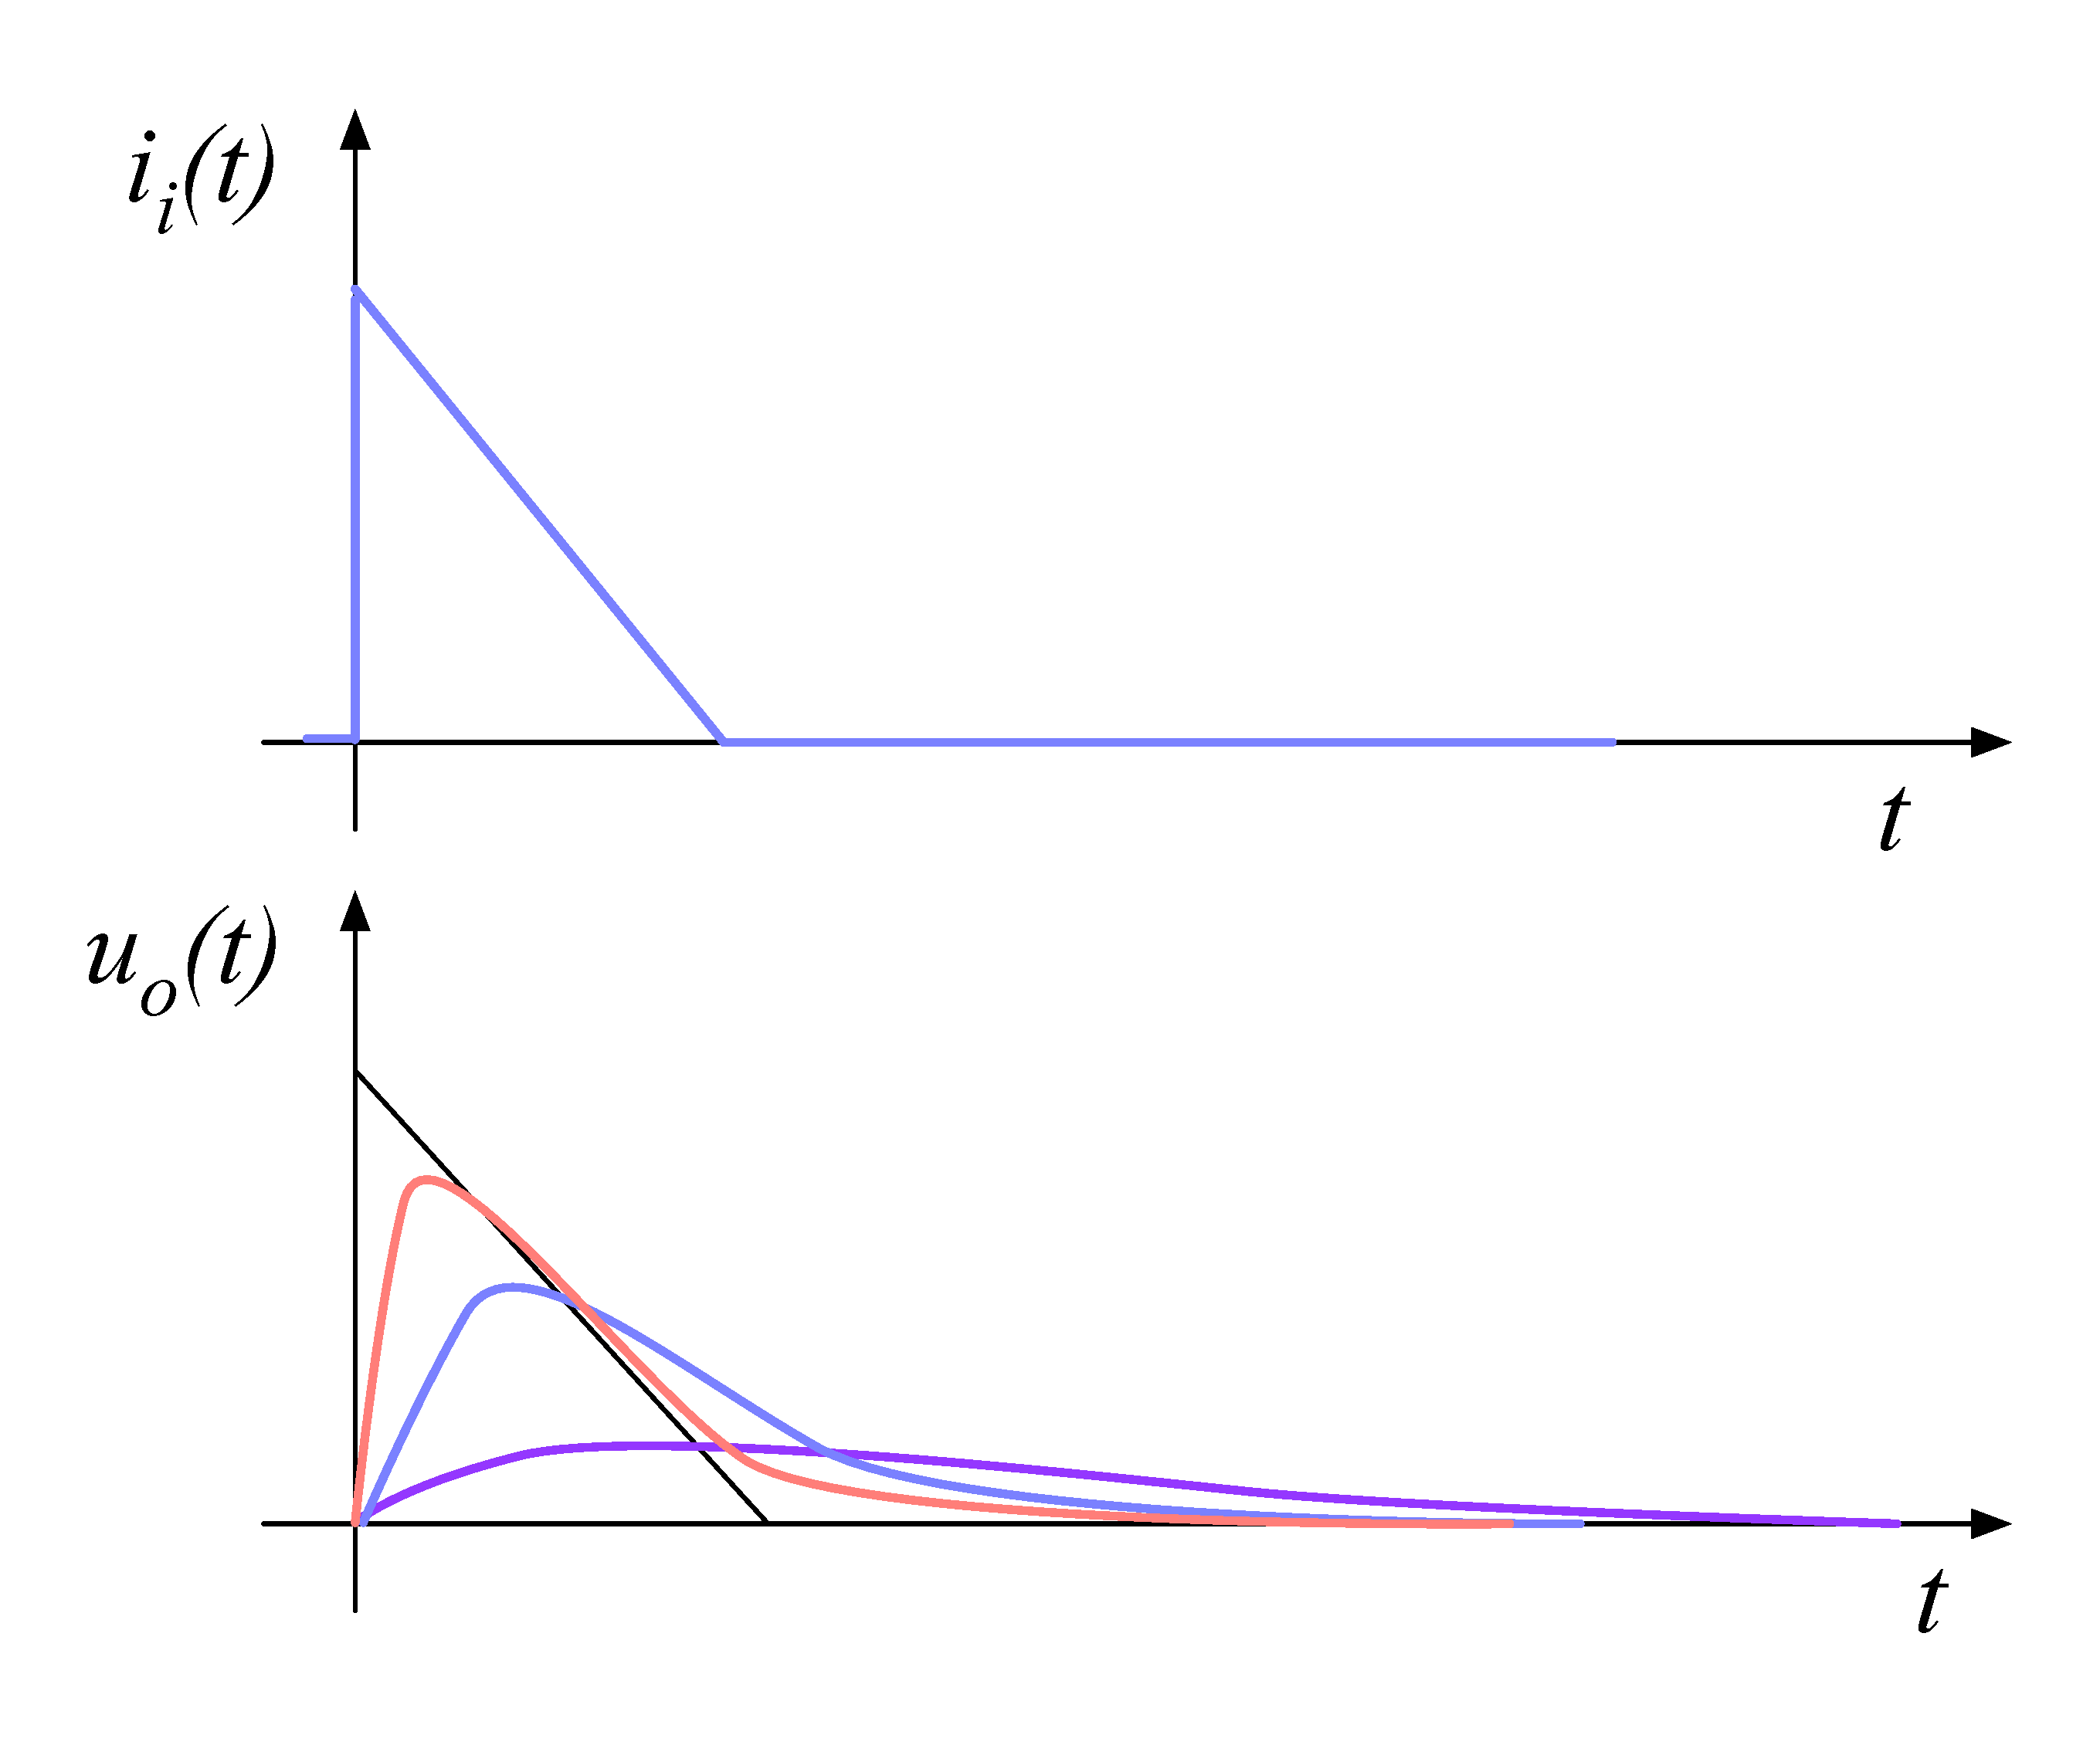
\includegraphics[width=0.8\linewidth]{02_pulse_formation/pics/plots/currrc}
\caption{Input and output signal of the current amplifier.}
\label{fig:currc}
\end{center}
\end{figure}




\subsubsection{Charge-sensitive amplifier}
%(0.5 pg)
In order to measure integrated charge in the sensor, a feedback loop is added to the amplifier, as shown in figure~\ref{fig:chgamp}. The feedback can be used to control the gain and input resistance, as well as to integrate the input signal. The charge amplifier is in principle an inverting voltage amplifier with a high input resistance. 
 
In an ideal amplifier the output voltage $u_\mathrm{o}$ equals $-Au_\mathrm{i}$. Therefore the voltage difference across the capacitor $C_\mathrm{f}$ is $u_\mathrm{f}=(A+1)u_\mathrm{i}$ and the charge deposited on the capacitor is $Q_\mathrm{f}=C_\mathrm{f}u_\mathrm{f} = C_\mathrm{f}(A+1)u_\mathrm{i}$. Since no current can flow into the amplifier, all of the signal current must charge up the feedback capacitance, so $Q_\mathrm{f} = Q_\mathrm{i}$.

In reality, however, charge-sensitive amplifiers respond much slower than is the duration of the current pulse from the sensor. In addition, a resistor is added to the feedback line in parallel to the capacitor. The resistor and capacitor define the decay time constant of the pulse, as shown in figure~\ref{fig:chgrc}. This is necessary to return the signal to its initial state to be ready for a new measurement.
\begin{figure}[!t]
\begin{center}
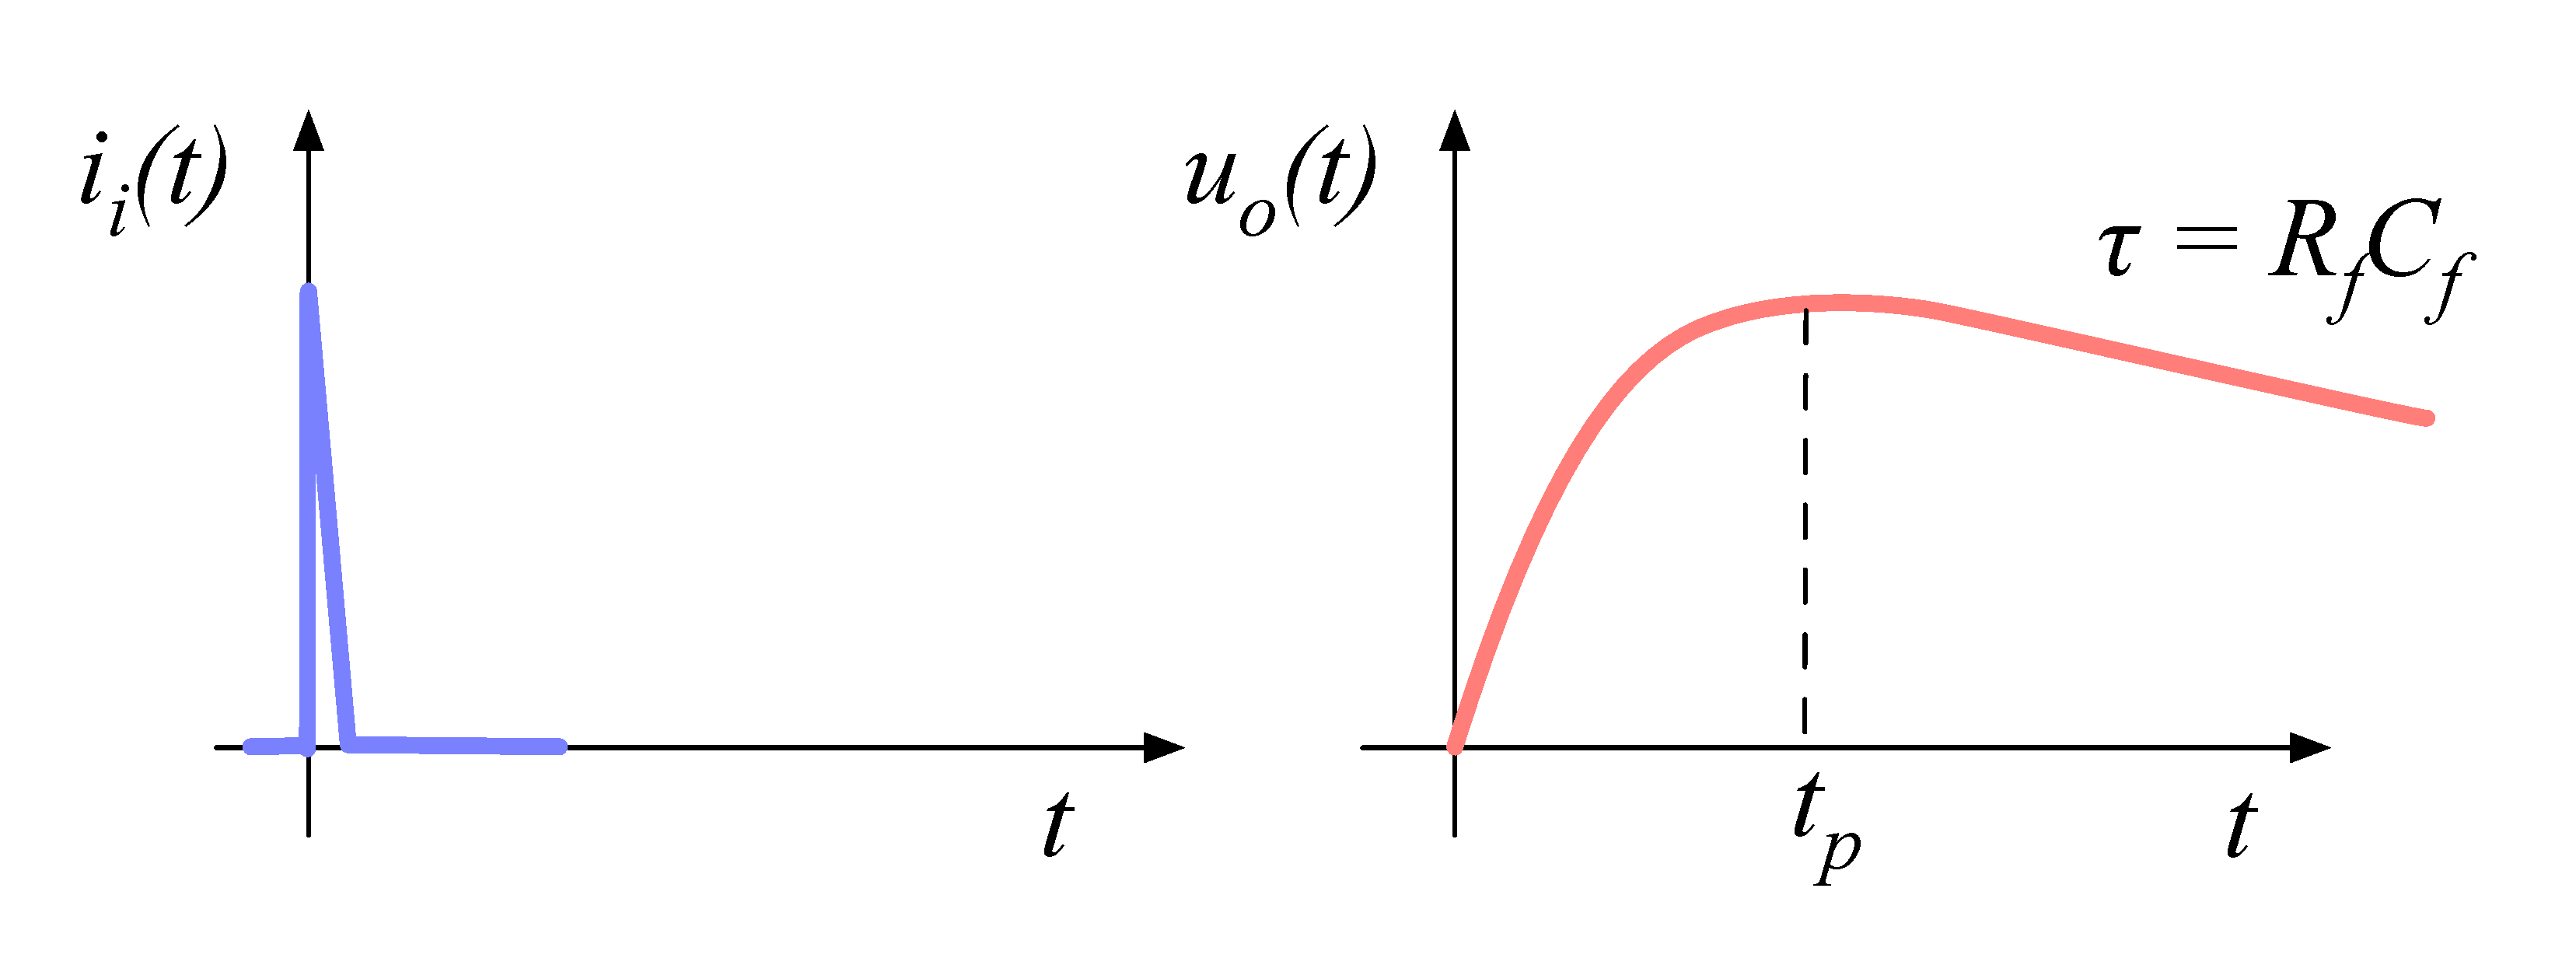
\includegraphics[width=0.7\linewidth]{02_pulse_formation/pics/plots/chgrc}
\caption{Input and output signal of the charge amplifier.}
\label{fig:chgrc}
\end{center}
\end{figure}

\subsubsection{Analogue electronic noise}
%(2 pg)
The electronic noise determines the ability of a system to distinguish differentsignal levels. The analogue signal contains ample information about the type and energy of incident radiation, which can quickly be erased or altered if the signal properties change. Therefore the noise contributions to the signal must be well understood to qualify the information the signal is carrying. The important contributions are listed below. Thermal or Johnson--Nyquist~\cite{} noise is the dominant noise contribution in the use case for diamond detector signal amplification and therefore defines the limitations of the detector system. This noise type is generated by the random thermal motion of charge carriers. The frequency range of the thermal noise is from 0 to $\infty$ with a predominantly uniform distribution. Therefore this is nearly a white noise. The resulting signal amplitude has a Gaussian distribution. The RMS of the noise amplitude is defined as
\begin{equation}
\label{eq:thermnoise}
u_\mathrm{RMS}=\sqrt{4k_BRT\Delta f}
\end{equation}
where $k_\mathrm{B}$ is the Boltzmann constant, $R$ is the input resistance of the amplifier, $T$ its temperature and $\Delta f$ the frequency range. This equation shows that it is possible to reduce the noise RMS by either (1) reducing the frequency range, (2) reducing the resistance of the conductor or (3) cooling the conductor. 

Contributions of shot noise, flicker noise and burst noise and other types are not significant relative to the thermal noise. However, the contributions of external factors can severely deteriorate the signal. This means the noise produced by capacitive or inductive coupling with an external source, which causes interference in the signal. These effects can be reduced by shielding the electronics and avoiding ground loops. 

\subsection{Analogue-to-digital converters}
An analogue-to-digital converter (ADC) is a device that converts the analogue electrical signal on the input to its digital representation - a series of digital values. This involves a quantisation -- \emph{sampling} of the signal at a defined sampling period, resulting in a sequence of samples at a discrete time period and with discrete amplitude values. The resolution of the ADC is the number of output levels the ADC can quantise to and is expressed in bits. For instance, an ADC with a resolution equal to $n=8$~bit  has a dynamic range of $N=2^n=256$~steps. The resulting voltage resolution $Q_\mathrm{ADC}$ at the input voltage range of $V_\mathrm{ADC}=\pm$50~mV is then
\begin{equation}
\label{eq:mvpercnt}
Q_\mathrm{ADC}=\frac{V_\mathrm{ADC}}{2^{n}}  = \frac{100~\mathrm{mV}}{2^8~\mathrm{bit}} = 0.39~\mathrm{mV/bit}.
\end{equation} 
With a sampling period of $t_\mathrm{s}=$1~ns the sampling rate is $f_\mathrm{s}=$1~GS/s (gigasample per second).
\begin{figure}[!t]
\begin{center}
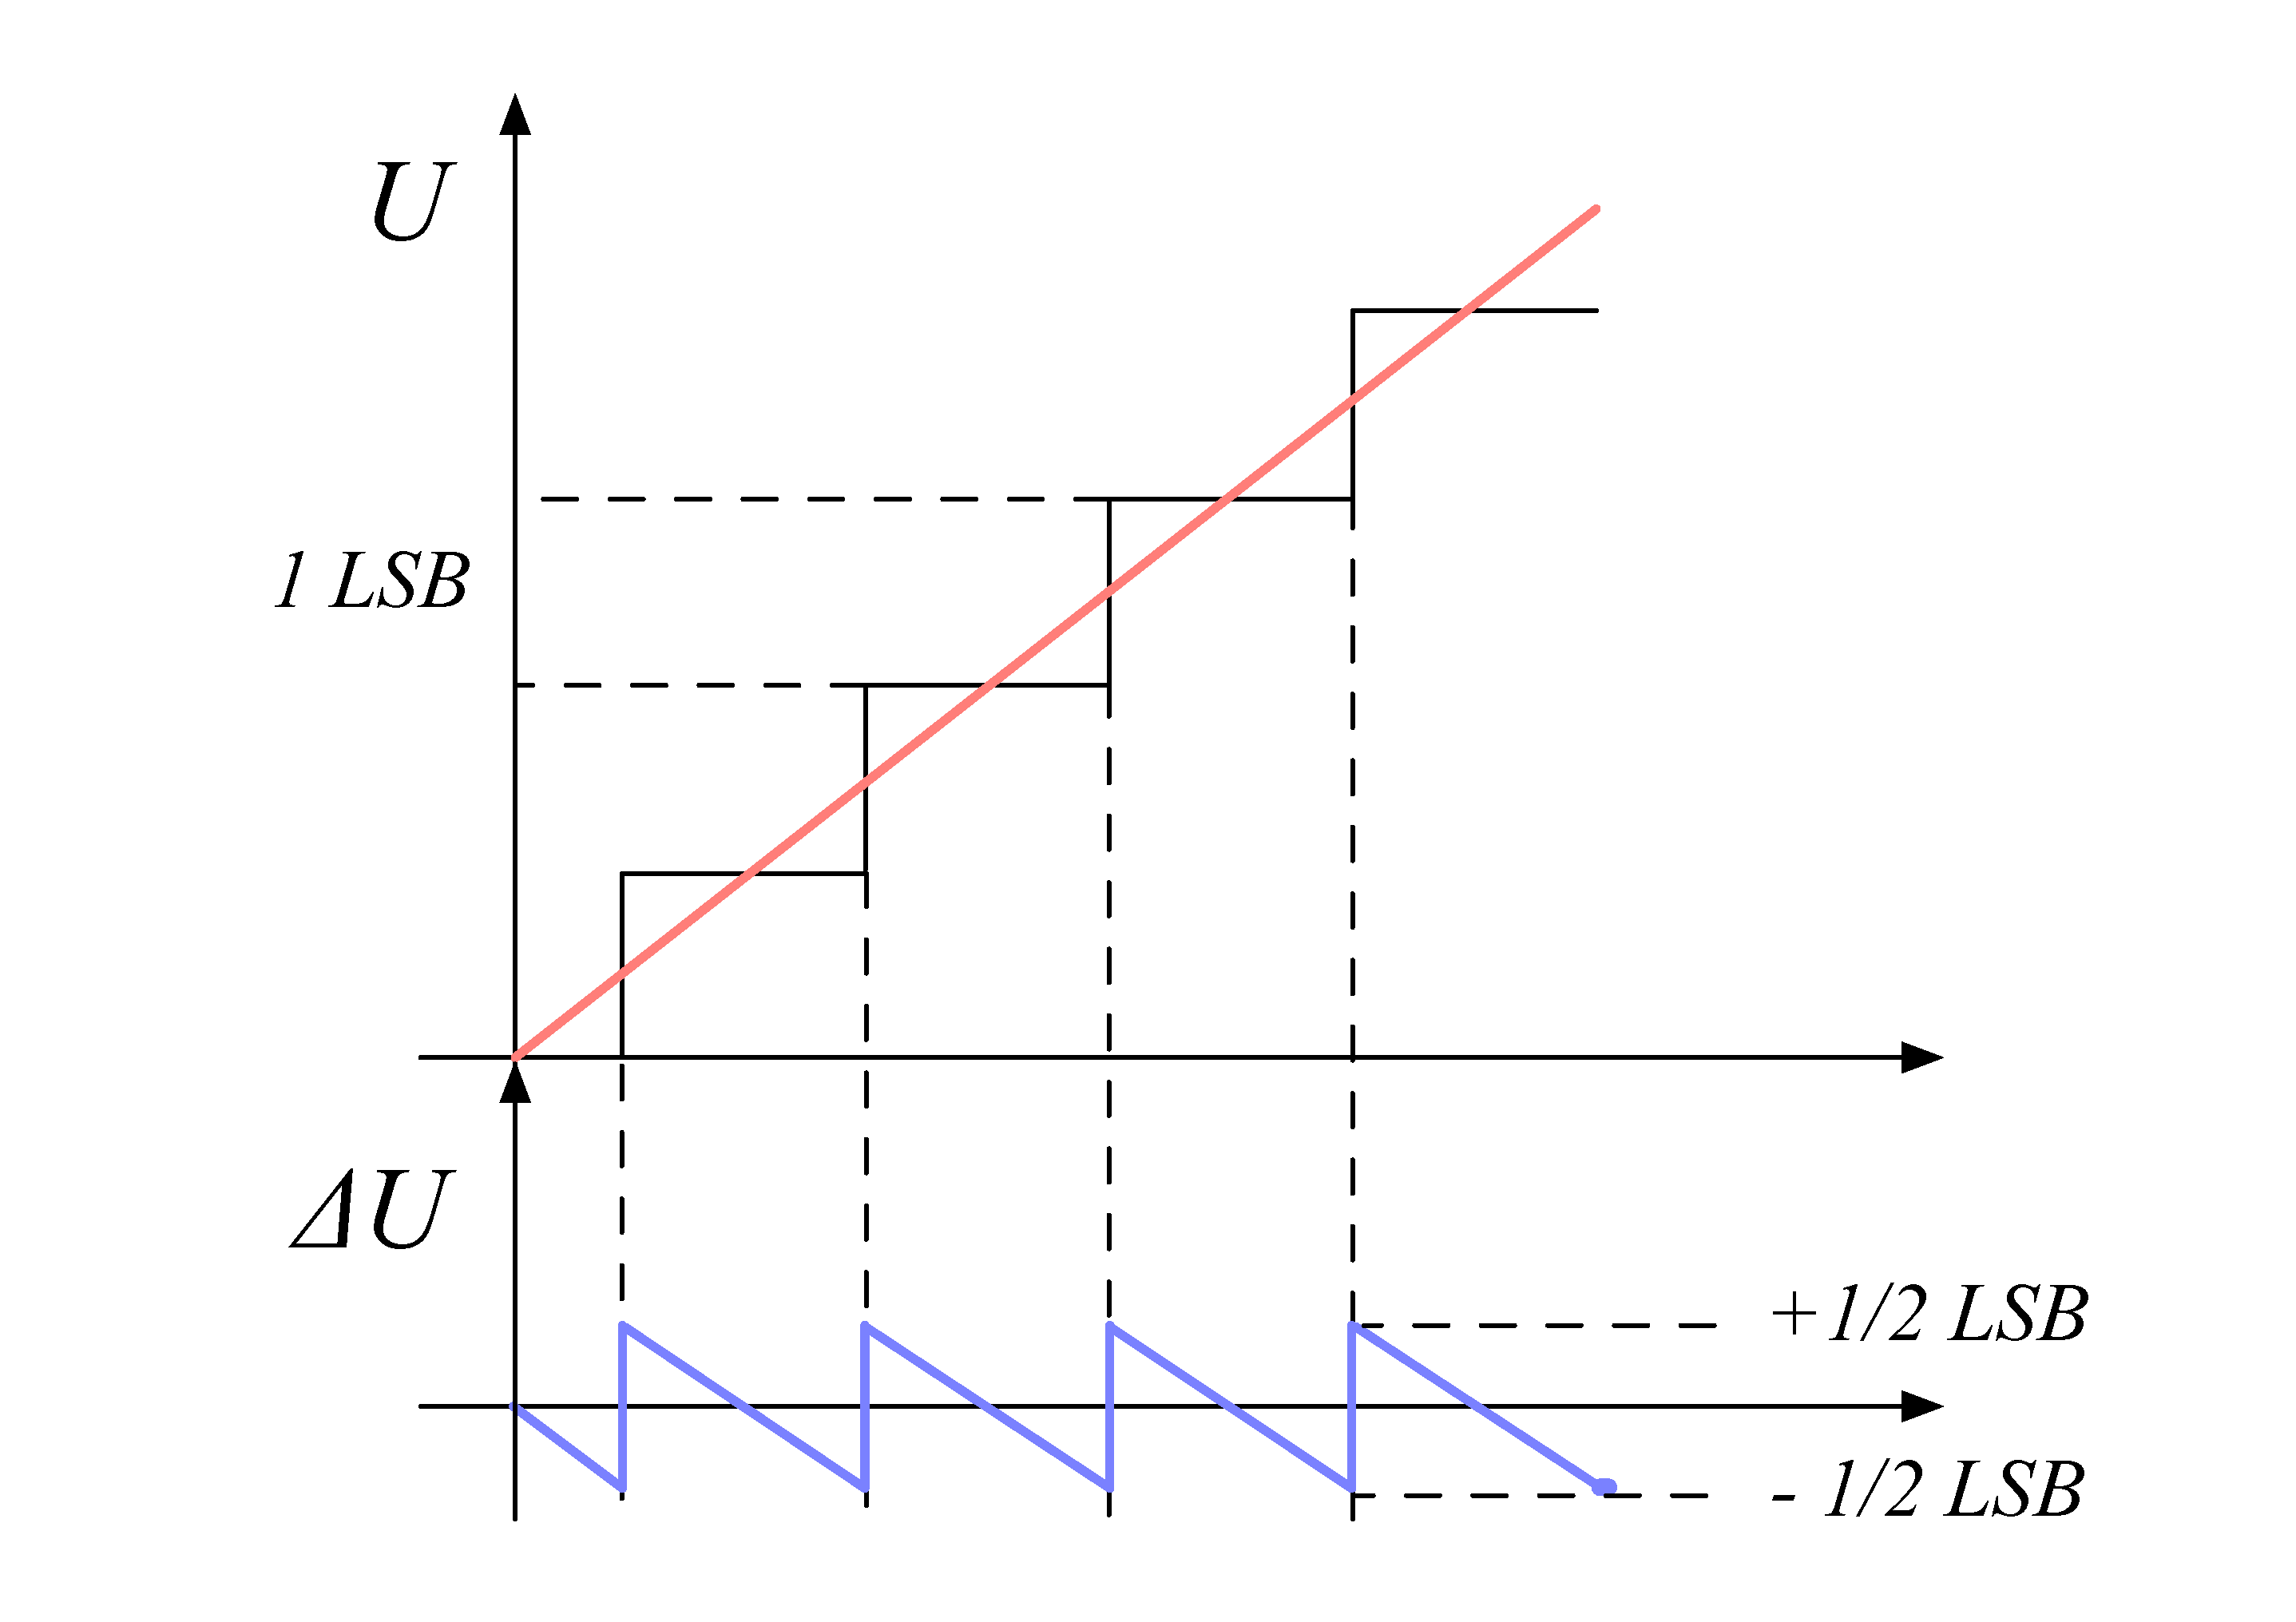
\includegraphics[width=0.7\linewidth]{02_pulse_formation/pics/plots/qerr}
\caption{Input signal digitisation and quantisation error.}
\label{fig:qerr}
\end{center}
\end{figure}

\begin{description}
\item[Quantisation error and quantisation noise] (or a round-off error) is a contribution to the overall measurement error due to digitisation (rounding). The quantisation error is defined as a difference between the actual analog value and the closest digitised representation of this value, therefore by the least significant bit (LSB), as seen in figure~\ref{fig:qerr}. The input signal amplitude is typically much larger than than the voltage resolution. In this case the quantisation error is not directly correlated with the signal and has an approximately uniform distribution~\cite{}. The probability density function $P(x)$ therefore has a rectangular shape bounded by ($-\frac{1}{2}$LSB, $\frac{1}{2}$LSB): 
  \begin{numcases}{P(x)=}
  \frac{1}{\mathrm{LSB}}, & $-\frac{1}{2}\mathrm{LSB}<= x <=-\frac{1}{2} \mathrm{LSB}$  \\
  0, & otherwise.
  \end{numcases}
The height equal to $\frac{1}{\mathrm{LSB}}$ preserves the integrated probability of 1. The variance of the distribution is
\begin{equation}
\label{eq:intprob}
\sigma^2 = \int P(x) (x-\mu)^2 \mathrm{d}x.
\end{equation} 
The population mean is $\mu=0$, therefore
\begin{equation}
\label{eq:intprob2}
\sigma^2 = \int_{-\frac{1}{2}\mathrm{LSB}}^{\frac{1}{2}\mathrm{LSB}} \frac{1}{\mathrm{LSB}} x^2 \mathrm{d}x 
= \frac{x^3}{3\mathrm{LSB}} \Bigg|_{ -\frac{1}{2}\mathrm{LSB} }^{\frac{1}{2}\mathrm{LSB} }
= \frac{\mathrm{LSB}^2}{12}.
\end{equation} 
The RMS of the quantisation noise is defined as the square root of the variance: 
\begin{equation}
\label{eq:qerr}
\Delta Q_\mathrm{ADC}=\sqrt{\sigma^2} =  \frac{1}{\sqrt{12}}\mathrm{LSB}\sim0.289~\mathrm{LSB}.
\end{equation} 
For the example above the quantisation error equals $\Delta Q_\mathrm{ADC}=0.289\cdot 0.39$~mV~$=0.11$~mV. The error depends strongly on the linearity of the ADC, but this is out of scope of this document as the devices used have ADCs with a very good linearity.
\end{description}

\subsection{Digital signal processing}
The digitised signal can be processed to extract useful information. Therefore after the signal amplification and digitisation the signal is routed in a device which handles the digital analysis. The signal can either be processed immediately (in real time) or it can be saved to a data storage for analysis at a later stage (offline). The devices carrying out the processing can be multipurpose (e.g. Field Programmable Gate Arrays) or dedicated (e.g. Application-Specific Integrated Circuits).

\begin{description}
\item[Field Programmable Gate Array] (FPGA) is an integrated circuit designed to be reprogrammable and reconfigured after manufacturing. It consists of a set of logic gates that can be interconnected in numerous combinations to carry out a set of logic operations. Many such logic operations can take place in parallel, making the FPGA a powerful tool for signal processing. FPGAs are often used during system development or in systems in which the requirements might change with time. They can be reprogrammed in the order of seconds. In addition, the logic design only needs minor changes when migrating to a newer version of the FPGA chip of the same vendor. The FPGAs also offer faster time-to-market with comparison to application-specific solutions, which have to be developed. On the other hand, the price per part can be significantly higher than for the application-specific solutions. Also, their other major disadvantages are a high power consumption and a relatively low speed as compared to more application-specific solutions. However, today's solutions are capable of clock speeds higher than 500~MHz. Together with the integrated digital signal processing blocks, embedded processors and other modules, they are already very powerful and versatile. All in all, FPGAs are a good choice for prototyping and limited production, for projects with limited requirements for speed and complexity.

\item[Application-Specific Integrated Circuit] (ASIC) is an integrated circuit designed for a specific use. The design cannot be modified after chip production, as is the case with FPGAs. On the other hand, the ASICs can be optimised to perform a required operation at a high speed and at a low power consumption. In addition, due to the specific design the size of the chip can be much smaller. ASICs can be designed as hybrid chips, containing both a digital and an analog part. Finally, ASICs can be designed to withstand much higher irradiation doses than FPGAs and can therefore be used in harsh environments like in space or in particle colliders.

To update the chip, the design has to be submitted to a foundry, which produces the new chips with a turnover time of 4---6 weeks. The costs of a submission start at \$~50\,000, but the price per part can be reduced significantly with a high volume. To sum up, ASICs are used for high volume designs with well defined requirements where some stringent constraints in terms of power consumption and speed have to be met.
\end{description} 

\begin{figure}[!t]
%\centering
\begin{tabular}{cccc}
\subfloat{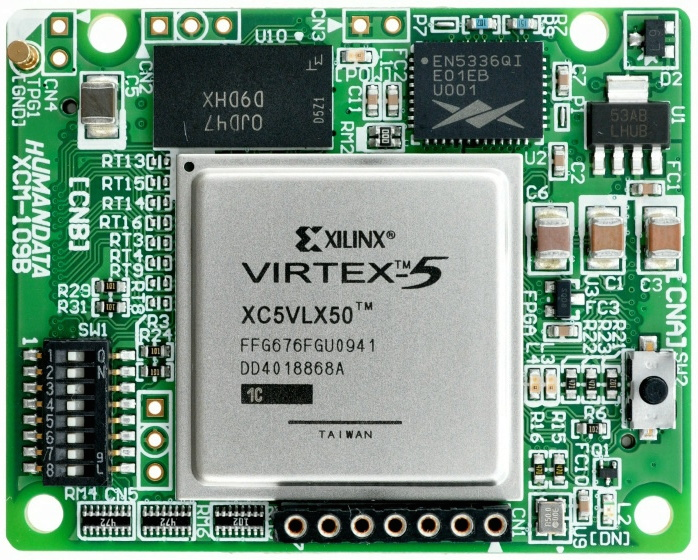
\includegraphics[width=0.47\textwidth]{02_pulse_formation/pics/fpga} \label{fig:fpga}} & 
\subfloat{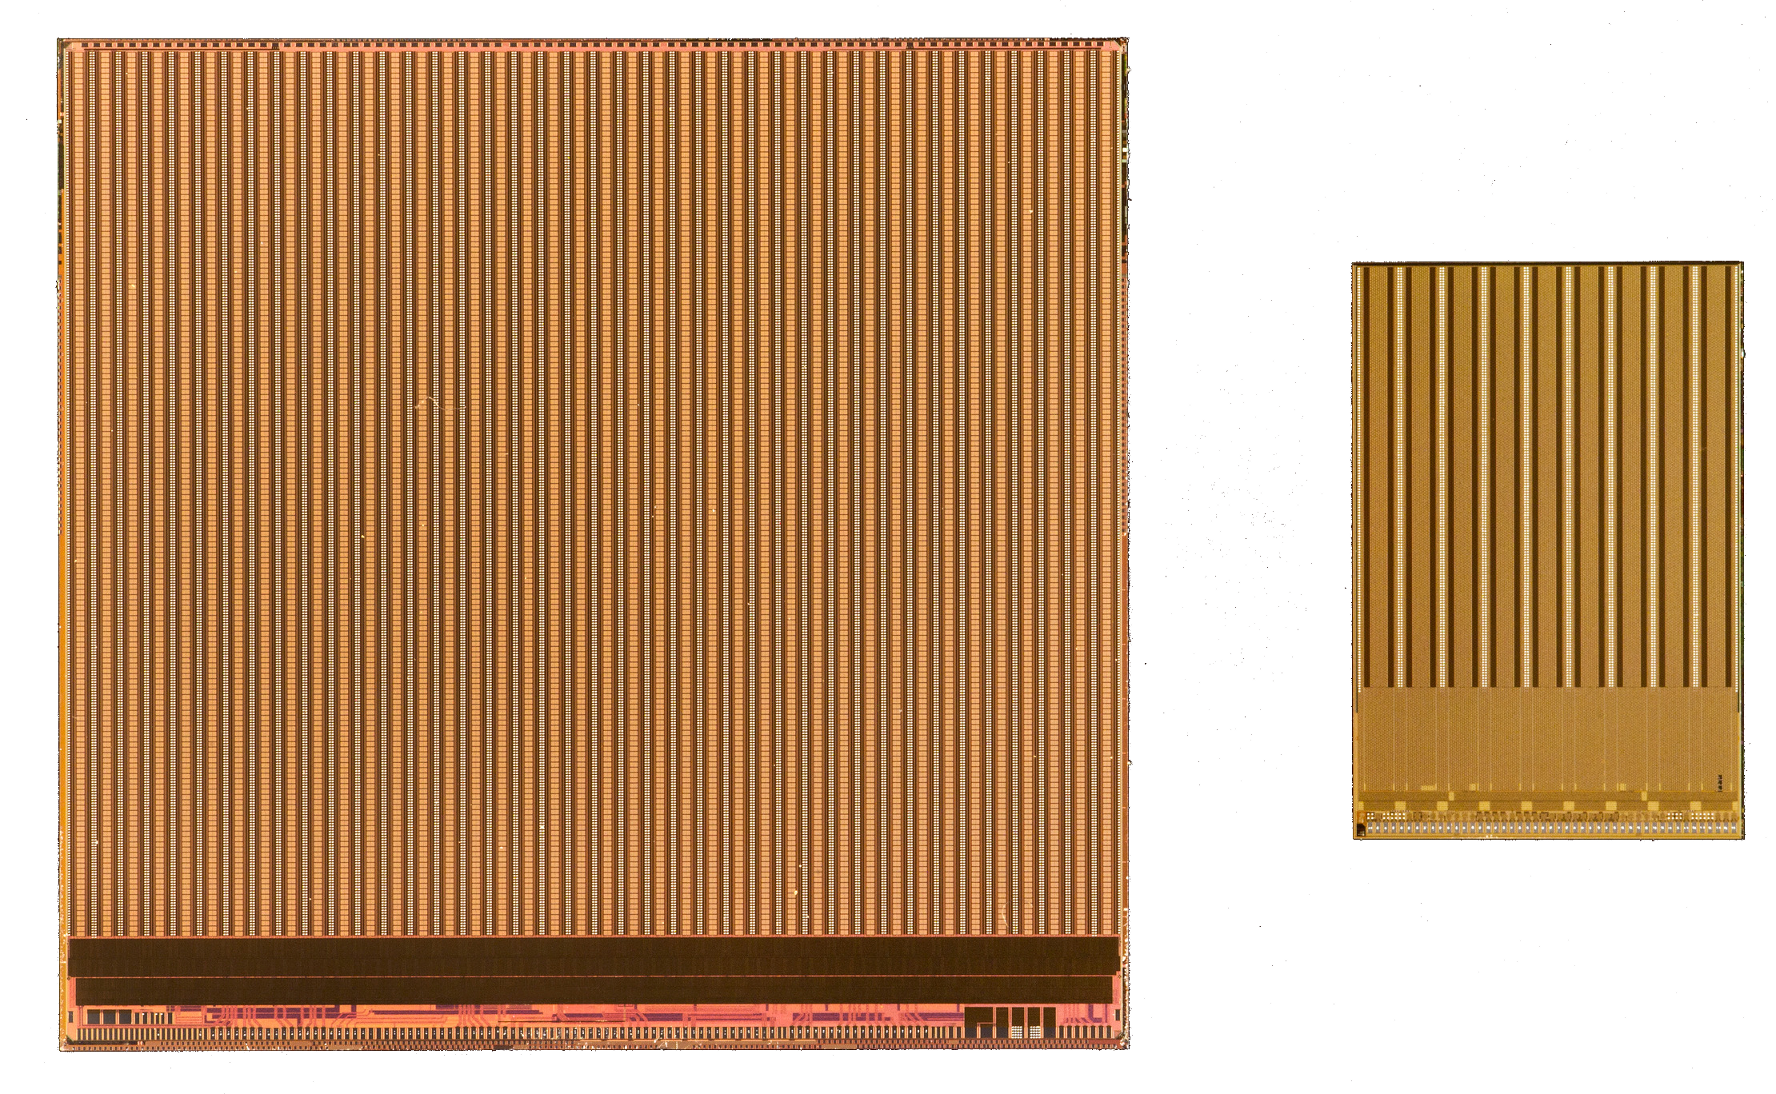
\includegraphics[width=0.47\textwidth]{02_pulse_formation/pics/asic2}  \label{fig:asic}}
\end{tabular}
\caption{An example of a Xilinx Virtex 5 FPGA~\cite{FPGA:00000} and an FE-I4 and FE-I3 ASIC chip~\cite{ASIC:00000}.}
\end{figure}


% ---------------------------- comment out when compiling the full document -------------------
\documentclass[twoside,12pt]{packages/mytustyle}  % default square logo 
\usepackage{amssymb}
\usepackage{caption}
\usepackage{upgreek}
\usepackage{subfig}
\usepackage{enumitem}
\setlist[description]{leftmargin=0cm,labelindent=0cm}

\usepackage{packages/fancyhdr}% http://ctan.org/pkg/fancyhdr
\pagestyle{fancy}% Change page style to fancy
\fancyhead[OR]{\renewcommand\thesection}
\fancyhead[ER]{\renewcommand\chaptername}
\newcommand\Chapter[2]{\chapter
  [#1\hfil\hbox{}\protect\linebreak{\itshape#2}]%
  {#1\\[2ex]\Large\itshape#2}%
}


%\fancyhf{}% Clear header/footer
%\fancyhead{}
%\fancyhead[RO, LE]{Experimental results}
%\fancyfoot{}
%\fancyfoot[RO, LE]{\thepage}% \fancyfoot[R]{\thepage}
\renewcommand{\headrulewidth}{0.7pt}% Default \headrulewidth is 0.4pt
%\renewcommand{\footrulewidth}{0.7pt}% Default \footrulewidth is 0pt
%\rfoot{\thepage}
\usepackage{lineno}
  \linenumbers

\begin{document}
\baselineskip=15pt
% ---------------------------------------------------------------------------------------------------------------

\tableofcontents

% ---------------------------------------------------------------------------------------------------------------
\Chapter{Experimental results}{Diamond irradiation study}
% ---------------------------------------------------------------------------------------------------------------

%Noise limitations
%
%Lab measurements
%
%Temperature and radiation limitations
%
%Transient current technique
%
%Charge - before and after irradiation
%
%compare with RD42 results
%
%Generation of trapping centres, reference KIT, Marok, Harris�
%
%IIa

This chapter contains the measurement results of data taken with diamond sensors. First the measurement setup is described (section~\ref{sec:meassetup}). Then the measured particle spectra are shown in~\ref{sec:pulsespectra}. This is followed by a study of effects of irradiation damage on the electrical signal of the diamond detector and its lifetime. The last section shows the results of the measurements of irradiated diamond samples at cryogenic temperatures. The aim of these studies is to find the operational limitations of diamond detectors for spectroscopy and tracking applications. The studies compare the experimentally acquired data with the theory from the previous chapter and define limitations of the diamond detectors in terms of noise, radiation and temperature.

Diamond sensors are mainly used for two types of measurements: particle counting and spectroscopy. The first type of measurements depends on the sensor's efficiency -- the ability to detect all or at least a known percentage of radiation quanta (particles or photons) that hit it. The energy of the radiation is not so important; what bears the information is the rate and the spatial distribution. Here the radiation does not necessarily stop in the bulk, but rather continues its way. In spectroscopy, on the other hand, the idea is that a particle stops within the sensor, depositing all its energy, which is then measured via the freed charge carriers. The aim of the experiments described in this chapter is to:
\begin{enumerate}[itemsep=0.1\baselineskip]
\item Quantify the efficiency of the sCVD diamond in counting mode, 
\item Quantify the degradation of efficiency  with respect to the received radiation dose,
\item Quantify the macroscopic effects on charge carrier behaviour with respect to the received radiation dose and 
\item Define limitations for its use in spectroscopy.
\end{enumerate}
The results discussed here show that there are several limitations for using diamond as a measurement device. All of them need to be taken into account for the measurement device to perform reliably and stably. The first step is to build a setup that is insensitive to external electromagnetic interferences and minimises electrical noise in the system. The setup needs to be calibrated before use. Then, the measurement conditions have to be defined, such as the temperature, the type of radiation and its flux. This allows us to estimate the lifetime of the detector and predict the longterm change of the signal. This change can then be accounted for when interpreting the output data. 






%\tableofcontents


% ---------------------------------------------------------------------------------------------------------------
%\clearpage
\section{Measurement setup}
\label{sec:meassetup}
% ---------------------------------------------------------------------------------------------------------------
To get reliable measurement results, great care has to go towards designing a measurement setup that minimises the noise in the measurements. Shielding has to be applied wherever possible. For instance, aluminium foil can be wrapped around the exposed parts of the system to shield them from external radio-frequency (RF) interferences. In addition, the sensors have to be covered to prevent the light from shining directly onto them. The incident photons can deposit enough energy to increase the leakage current of the detector.

The measurements using diamond that are explained in these chapters were carried out using several measurement setups, but they are all similar in terms of the electrical signal chain. The measurement chain consists of three main parts: a diamond sensor, a signal preamplifier and a readout device, asequi seen in diagram~\ref{fig:ro-chain}. The signals propagating along the analogue chain (before being digitised by the readout device) are fast -- in the GHz bandwidth range --  and with low amplitudes -- of the order of tens of $\upmu$V. This gives rise to importance of RF shielding. Also, the connection between the carrier and the preamplifier has to be as short as possible to avoid capacitive signal losses in the transmission line. Finally, the system needs to be grounded properly.

\begin{figure}
\centering
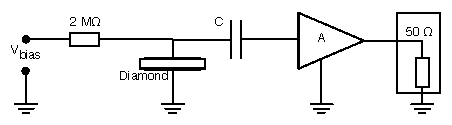
\includegraphics[width=0.8\textwidth]{plots/ro-chain}
\caption{Diagram of a diamond detector readout chain.}
\label{fig:ro-chain}
\end{figure}


\subsection{Preamplifiers}
\label{sec:preamps}
Two preamplifiers are used for the measurements, one sensitive to charge and the other to current. \emph{CIVIDEC Cx} (figure~\ref{fig:ampcx}) is a charge sensing amplifier. Its high SNR (equivalent noise charge of 300~+~30~pF$^{-1}$~e$^-$ and a reported gain of $\sim$12~mV/fC) makes it a good choice for spectroscopic measurements with diamond sensors. \emph{CIVIDEC C2} (figure~\ref{fig:ampc2}) is a fast current preamplifier with a 2~GHz bandwidth limit. It is used for TCT measurements because if its fast response and a good SNR. Both are embedded in an RF-tight aluminium box to reduce the noise pickup. Both have an AC coupled input and an output with a  50~$\Upomega$ termination.

\begin{figure}[!t]
%\centering
\begin{tabular}{cccc}
\subfloat[Cx charge sensing preamplifier]{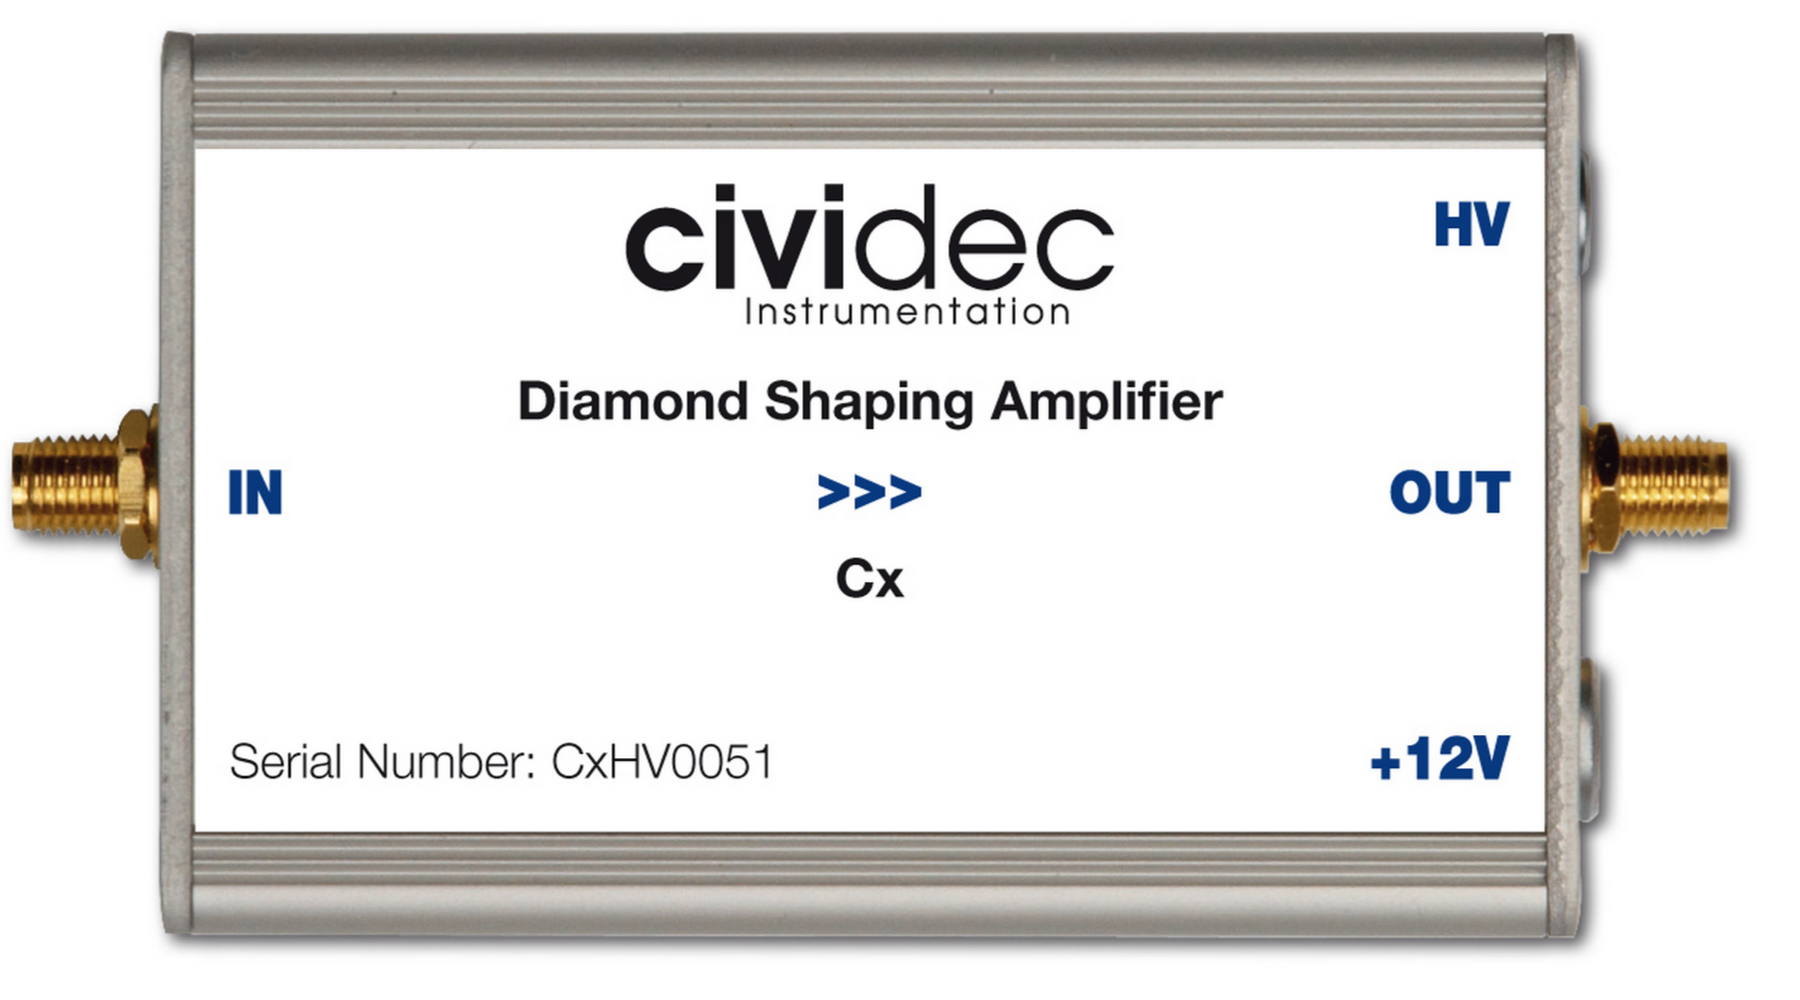
\includegraphics[width=0.45\textwidth]{pics/setup/Cx} \label{fig:ampcx}} &
\subfloat[C2 fast charge preamplifier]{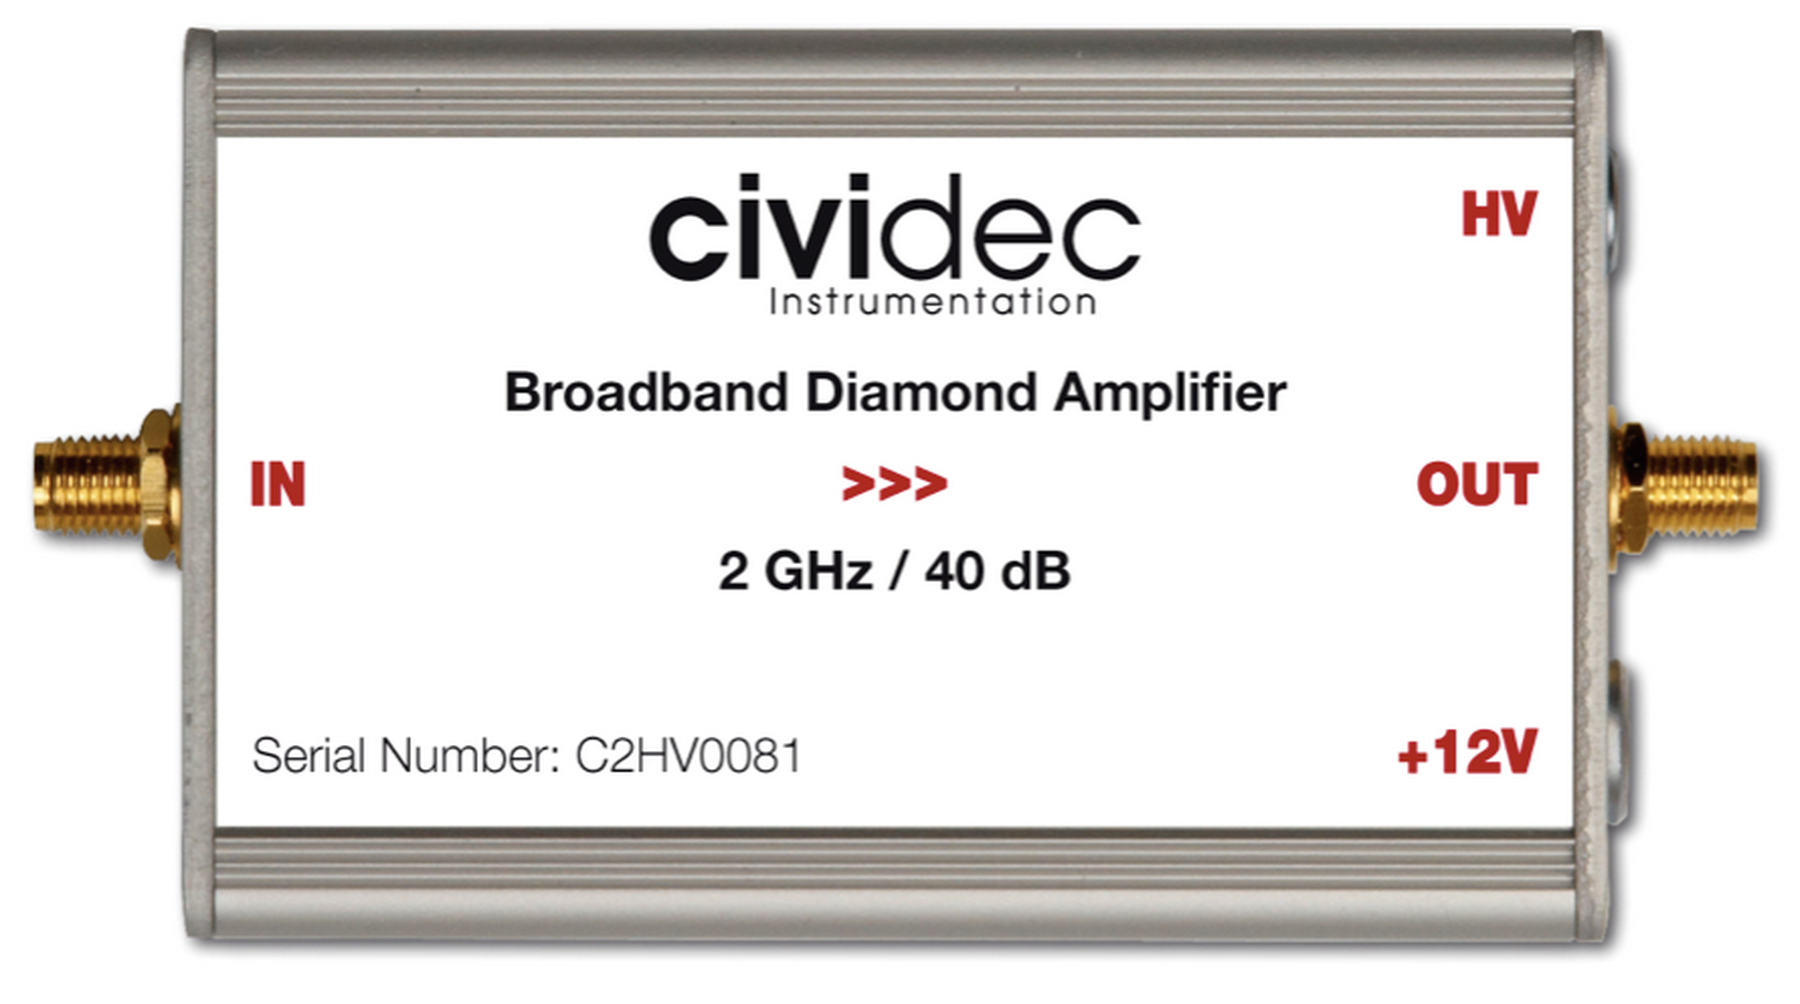
\includegraphics[width=0.45\textwidth]{pics/setup/C2}  \label{fig:ampc2}}
\end{tabular}
\caption{Amplifiers used for the charge and current measurements}
\end{figure}


\subsubsection{Calibration}
The amplifiers have to be calibrated before use to determine their gain. Both are calibrated using a square signal generator with a known amplitude step of $U_{\mathrm{in}}=(252\pm5)$~mV. A 2~GHz oscilloscope with a 10~GS/s sampling is used to carry out these measurements. 

In the case of the Cx charge sensitive amplifier, the signal is routed through a capacitor with a calibration capacitance $C_{\mathrm{cal}}=(0.717\pm0.014)$~pF and then to the input of the amplifier. The pulse area behind the capacitor is $a_{\mathrm{cal}}=(5.0\pm0.5)$~pVs, with the signal amplitude on the output amounting to $U_{\mathrm{C_x}}=(1.95\pm0.05)$~V. The input voltage step combined with the calibration capacitance yields a calibration charge $Q_{\mathrm{cal}}=C_{\mathrm{cal}}\cdot U_{\mathrm{in}}=(181\pm5)$~fC. The gain of the Cx amplifier is therefore $A^{\mathrm{Q}}_{\mathrm{Cx}}=\frac{U_{\mathrm{Cx}}}{Q_{\mathrm{cal}} }=(9.3\pm0.4)$~mV/fC or  $A^{\mathrm{a}}_{\mathrm{Cx}}=\frac{U_{\mathrm{Cx}}}{a_{\mathrm{cal}} }=(390\pm40)$~mV/pVs. The area-based amplification factor has a higher uncertainty ($\sim10~\%$) than the amplitude-based factor ($\sim4~\%$) due to the measurement limitations of the oscilloscope. Nevertheless, it can be used as an estimate for the integrated charge of a current pulse.

To calibrate the C2 current amplifier, only the amplitude gain has to be measured. The input signal amplitude has to be such that it keeps the output amplitude within the amplifier's linear range, that is $\pm1$~V. The signal from the generator is therefore routed through a 36~dB attenuator to decrease its amplitude to $U_{\mathrm{inAtt}}=(3.95\pm0.05)$~mV. Two amplifiers with different gains have been measured, because both are used for the measurements at different times. The output of the first amplifier amounts to $U_{\mathrm{C2-1}}=(860\pm5)$~mV. This yields the amplification gain equal to $A_{\mathrm{C2-1}}=\frac{U_{\mathrm{inAtt}}}{U_{\mathrm{C2-1}}} =(217\pm3)$. The second amplifier has the output equal to $U_{\mathrm{C2-2}}=(632\pm5)$~mV with the gain equal to $A_{\mathrm{C2-2}}=(152\pm3)$. 





\subsection{Diamond samples}
\label{sec:diamsam}
Detector-grade diamonds are very difficult to produce, mostly because it is very difficult to ensure a high enough purity of the lattice. %It takes companies years of trials to produce high enough quality product. Since the target market are almost exclusively particle physics research institutes, the companies work closely with them to make sure the product is up to par with the requirements. 
The sensor samples used for these studies were bought at Element Six (E6)~\cite{}. They all have the same standard dimensions. sCVD diamonds with dimensions $4.7\times4.7$~mm$^2$ are already sufficiently large for most of the beam monitoring applications and still affordable. 
%; the cost of sCVD diamonds grows exponentially with the area. There is also an ongoing race among the producers to produce larger and larger diamonds while maintaining the same cost. For instance, a new company IIa~\cite{} from Singapore has produced high-quality samples with larger dimensions and the diamond detector community is currently involved in extensive tests of their products. 
One of the samples with dimensions of $5.6\times5.3$~mm$^2$ produced by IIa Singapore~\cite{} was also sent to CERN to be characterised. The target thickness for all the samples is 500~$\upmu$m. Diamonds this thick yield a high enough signal-to-noise ratio for MIPs to be measured by the electronics.
\begin{figure}
\centering
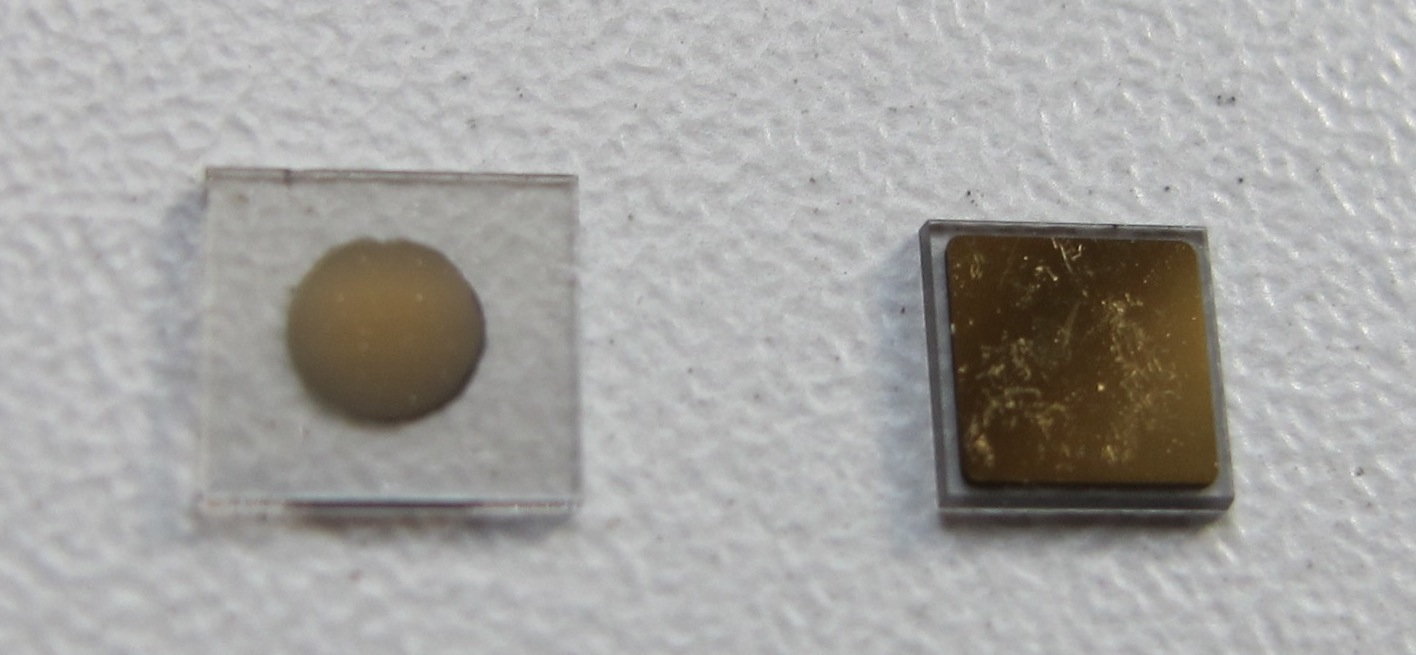
\includegraphics[width=0.8\textwidth]{pics/setup/diamond4}
\caption{Two scCVD diamond samples: A IIa 1scdhq (left) and an E6 S37 (right)}
\label{fig:diams}
\end{figure}
Table~\ref{tab:diamsamp} shows all the samples used for this study. Two of them were later irradiated with 300~MeV pions and then compared to the pre-irradiated state. Irradiation doses for damaging the material need to be high -- above $10^{12}$~particles per cm$^2$ to be able to observe change in the sensor's behaviour. 

\begin{footnotesize}
\begin{center}
\begin{tabular}{   l  c  c  c  c c c }
\hline
Name & Type &Producer & Dimensions [mm$^2$] & Thickness [$\upmu$m] & Electrode & Irradiatied \\
\hline
S37 & sCVD & E6 & $4.7\times4.7$ & 548 & Cr/Au & no \\
S50 & sCVD & E6 & $4.7\times4.7$ & 537 & Cr/Au & no \\
S52 & sCVD & E6 & $4.7\times4.7$ & 515 & Cr/Au & $1\times10^{14}~\uppi$~cm$^{-2}$ \\
S79 & sCVD & E6 & $4.7\times4.7$ & 529 & Cr/Au & $3.63\times10^{14}~\uppi$~cm$^{-2}$ \\
ELSC & sCVD & E6 & $4.7\times4.7$ & 491 & Cr/Au & no \\
1scdhq & sCVD & IIa & $5.6\times5.3$ & 460 & Cr/Au & no \\
\hline
\end{tabular}
\captionof{table}{Diamond sensor samples used}
\label{tab:diamsamp}
\end{center}
\end{footnotesize}
%_\mathrm{300~MeV}

The diamond samples have quoted impurity densities of $\leq2\times10^{14}$~cm$^{-3}$ and nitrogen incorporation of $\leq1$~ppb. The electrodes were added by various companies and institutes. For instance, S52 was metallised by a company DDL~\cite{} while the Physics Department of the University of Firenze, Italy metallised the S79. There are also several techniques for producing the electrodes. The DDL contacts consist of three layers: DLC (diamond-like carbon)/Pt/Au with 4/10/200 nm thicknesses, respectively. The metallisation for S79, on the other hand is made up of Cr/Au with a total thickness of $\sim$400~nm. The area coverage also differs from sample to sample. Diamonds must not be metallised until the very edge as the proximity of contacts with a high potential can lead to sparking. However, the areas not covered by the metallisation are less efficient because the fringe fields at the edges are not as strong as in the middle. This effectively reduces the sensitive area of the sensors. In the diamonds used here the effective area was anywhere from 9~mm$^2$ to 18~mm$^2$. Leakage current through the bulk was below 1~ns, but increased for the irradiated samples. The capacitance was of the order of (2.0$\pm$0.3)~pF.


\subsection{Readout devices}
\label{sec:readoutdev}
Electrical signals in diamond detectors are in the GHz frequency range. To preserve this information, the readout device has to have a high bandwidth limit. For instance, a 250~MHz limit is enough for the spectroscopic measurements with the Cx charge amplifier, but might be insufficient for the current measurements with the C2 amplifier. Two devices are used take data shown in this chapter. The first choice is a 2~GHz LeCroy WaveRunner 204MXi-A. This specific model has a high enough limit for the fast current preamplifier signals. It offers a versatile solution for analogue signal readout -- it is fast to set up and reliable. It is very convenient for use in lab tests and for experiments where small amounts of data are taken and where speed is not crucial. However, its slow acquisition speed turns out to be a bottleneck in the test beam experiment. Its initial 100~Hz readout rate decreases to a mere 20~Hz within 20 minutes, because every single trigger is saved as a separate file and the Windows operating system is not capable of handling 10000+ files in a single directory easily. This is why it has been exchanged with a DRS4~\cite{}, an analogue readout device developed by PSI, Switzerland. This compact device is capable of recording up to four waveforms at a time at a steady rate of up to 500~Hz. Its 700~MHz bandwidth limitation is sufficient for the signal from the charge amplifier.



\subsection{Setup for the efficiency study using $\upbeta$ particles}
The efficiency study of the diamond sensors has been carried out at CERN in the North Hall test beam facility. There a straight high-energy particle beam of $\uppi_\mathrm{120~GeV}$ is provided to the users to calibrate their detectors. The beam had a transverse spread of $\sigma=10$~mm in both axes. The particle rate is of the order of $10^4~\uppi$~cm$^{-2}$~s$^{-1}$. A diamond sensor embedded in a PCB carrier has been placed in the beam spot perpendicular to the beam and connected via an SMA connector directly to a charge amplifier (described below). The amplified signal is read out using a LeCroy oscilloscope and a DRS4 analogue readout system (both described below). A computer is used as a controller and data storage for the readout device. A beam telescope~\cite{} is used as a reference detector. It is a device that helps to cross-check the measurements of the devices under test (DUTs) and to carry out spatially resolved studies on the DUTs. It consists of several pixellated sensor planes placed in series, which can track a particle's trajectory with a precision of a few $\upmu$m. The sensor planes are positioned in front of the DUT and behind it. Then the beam telescope acts as a trigger system -- it triggers the readout of both the telescope data and DUT data when both the planes in front and behind the DUT recorded a hit by the impinging particle. A particle detected by all the planes within the DUT window and the DUT itself counts towards its efficiency whereas a hit missed by the DUT means that the DUT is not 100~\% efficient. To discard the hits that miss the DUT completely, a region of interest (ROI) can be chosen in the beam telescope planes. The equation for calculating the sensor efficiency is therefore
\begin{equation}
\label{eq:sensoreff}
\epsilon = \frac{ N_\mathrm{DUT} \wedge N_\mathrm{telescope} }{ N_\mathrm{telescope} }
\end{equation}
for an ROI smaller than the sensitive region of the diamond.


\subsection{Room temperature $\upalpha$-TCT setup}
This TCT study is a follow-up of an extensive diamond TCT study at cryogenic temperatures~\cite{}. The room-temperature TCT measurements have been carried out in the lab. The setup consists of a diamond sensor embedded in a PCB carrier, a current amplifier and an oscilloscope. To measure $\upalpha$ particles, their energy loss during their trajectory has to be minimised. Therefore the diamond is placed inside a vacuum chamber. The chamber is a steel tube with a diameter of 5~cm. On one side it is connected to a vacuum pump via an steel pipe. A feedthrough with an SMA connector is placed on the other side. A C2 current amplifier is connected directly onto the feedthrough. The amplified output is connected to the oscilloscope via an SMA cable. An $^{241}$Am source with a diameter of 2~cm and a height of 0.5~cm is fixed onto the sensor carrier (figure~\ref{fig:carrier}, figure~\ref{fig:carsrc}). Then the carrier is inserted in the chamber and fixed in place using an air-tight clamp. The pump can then be switched on. It is capable of providing the inside pressure as low as $10^{-4}$~mbar after approximately one hour of operation, but measurements can take place even after five minutes of evacuation, at around $10^{-3}$~mbar. The most important thing to bear in mind is to switch the bias voltage of the sensor OFF during the process of evacuation, because the gas becomes more conductive at the pressure of the order of $10^{-1}$~mbar~\cite{}. A failure to switch off the bias voltage may cause a spark between the signal and ground line, destroying the amplifier. 

\begin{figure}[!t]
%\centering
\begin{tabular}{cccc}
\subfloat[PCB carrier with an embedded diamond sample]{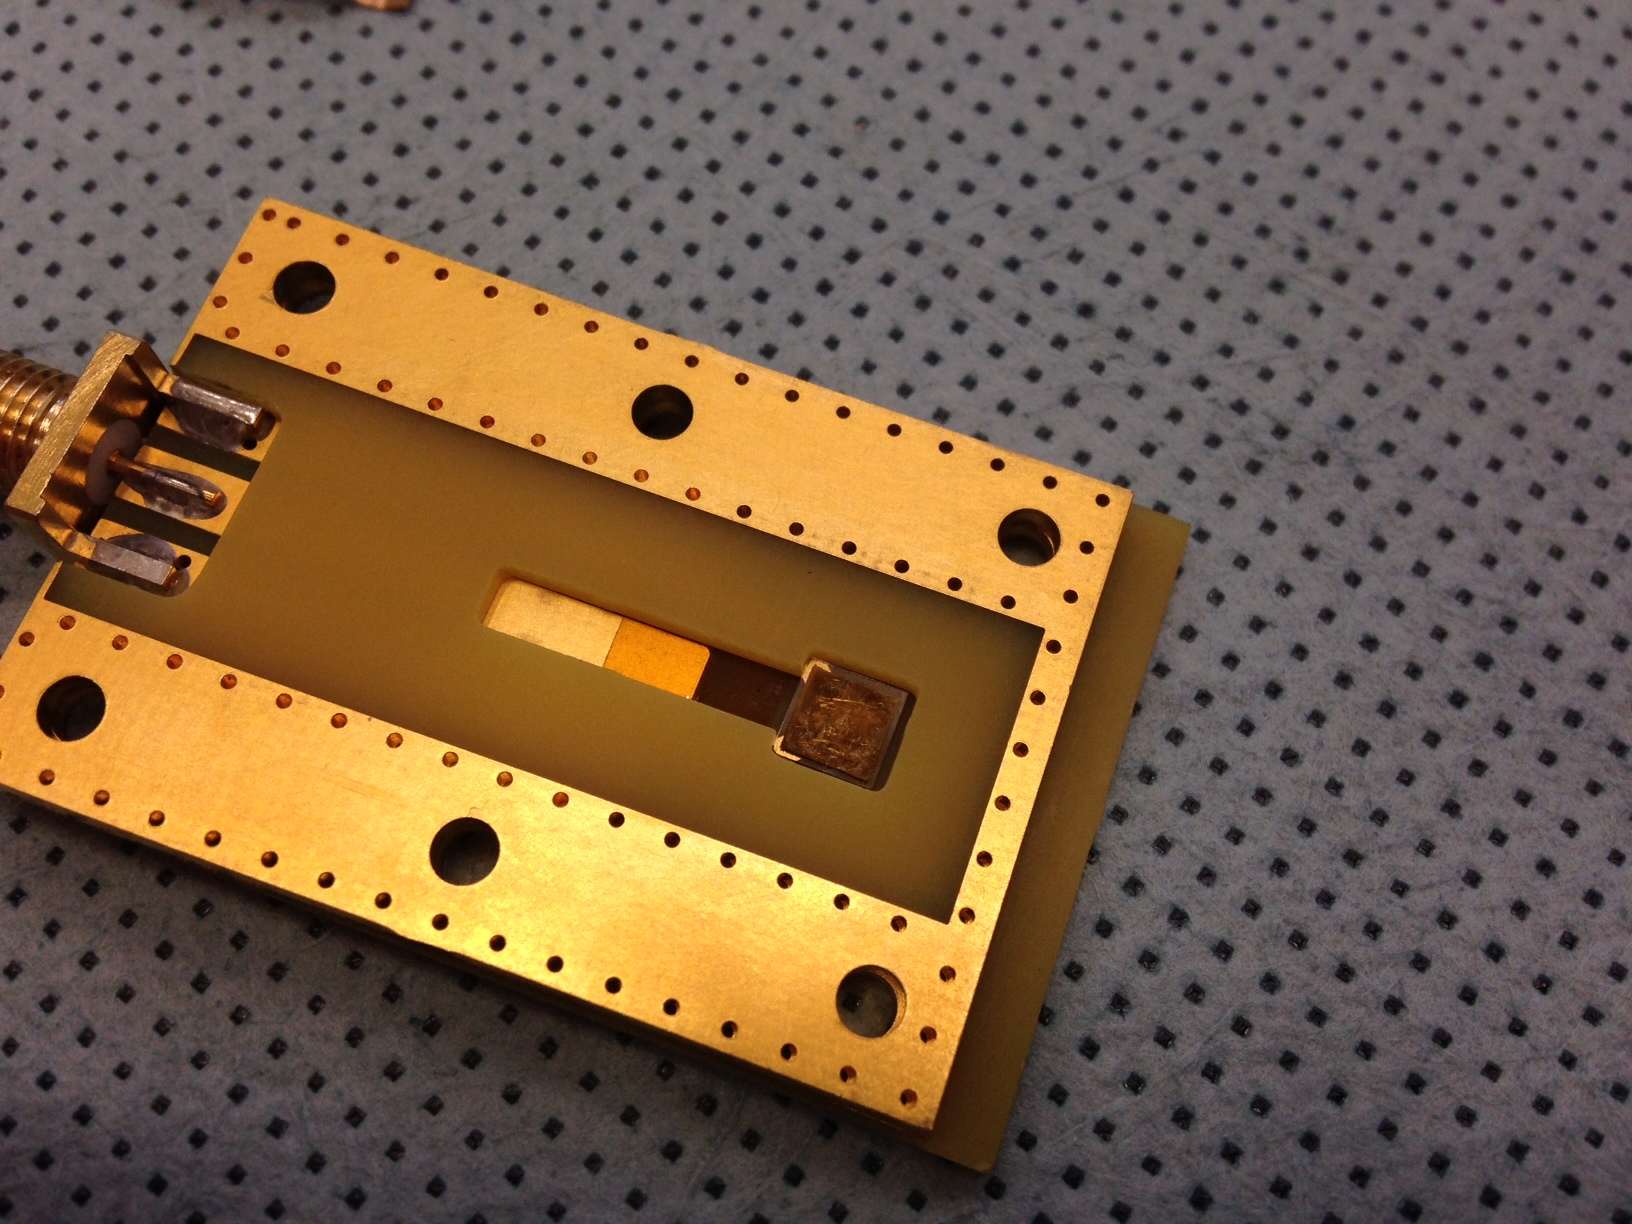
\includegraphics[width=0.45\textwidth]{pics/setup/carrier2} \label{fig:carrier}} &
\subfloat[Radioactive source over the carrier]{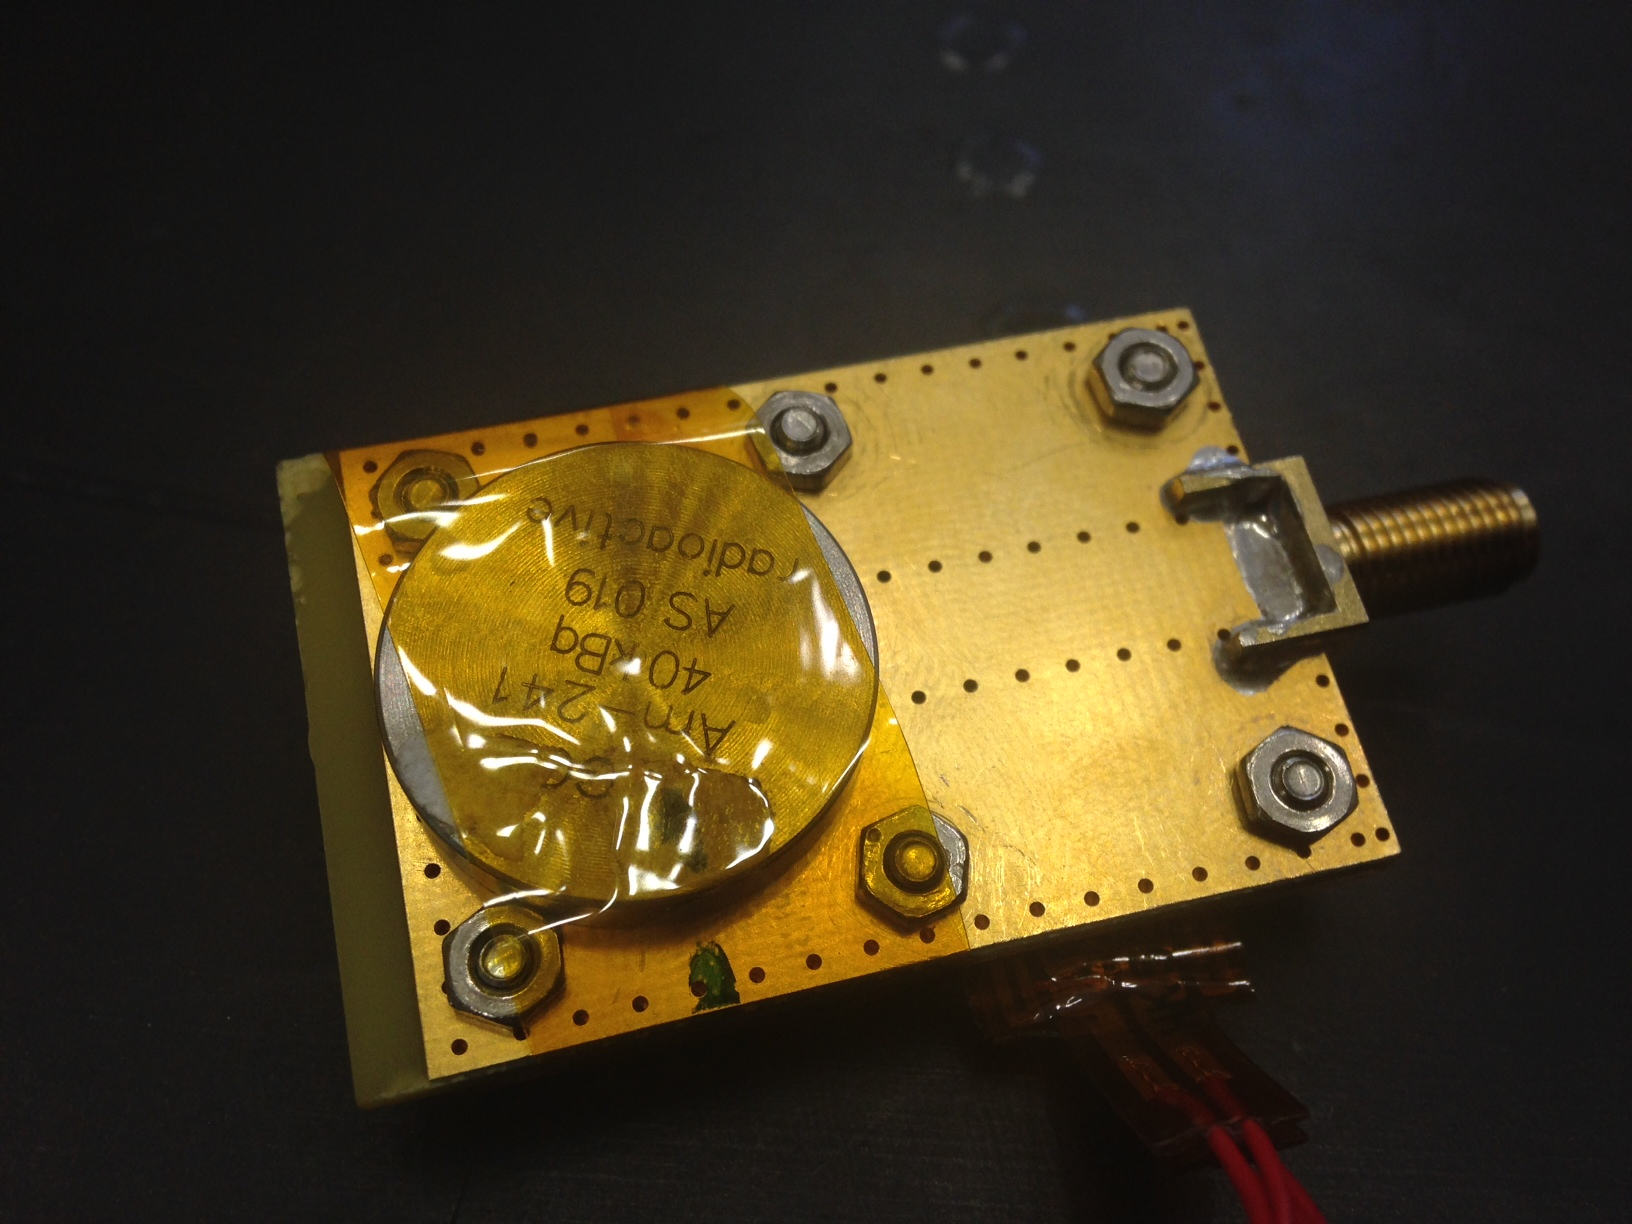
\includegraphics[width=0.45\textwidth]{pics/setup/carriersource2}  \label{fig:carsrc}}
\end{tabular}
\caption{Positioning of the $\upalpha$-source on top of the sensor carrier}
\end{figure}


\subsection{Cryogenic $\upalpha$-TCT setup}
\label{sec:cryosetup}
The experiment at cryogenic temperatures has been carried out in the cryolab at CERN. The room-temperature TCT setup has to be modified to allow for measurements at temperatures as low as 2~K. It consists of three parts: 
\begin{enumerate}
\item a cryostat --  a thermally insulated cylinder capable of containing liquid helium,
\item an inlet -- an air-tight mechanical tube with valves and feedthroughs at the top that is lowered in the liquid helium and
\item the diamond sample embedded in a PCB carrier with a fitted temperature sensor, a heater and cables leading to the feedthroughs.
\end{enumerate}
The setup is described in detail in~\cite{}.

When the diamond sample is placed in the PCB carrier and the $^{241}$Am source is in place, the inlet is sealed and lowered in the empty cryostat. Then the inside volume of the inlet is evacuated to down to $10^{-5}$~mbar while the liquid helium is flowing into the cryostat. To improve the thermal contact between the diamond and the coolant, a small amount of helium gas is added inside the evacuated inlet, setting the vacuum to around $10^{-3}$~mbar. This value changes with time, because the gas condenses on the walls of the inlet, reducing the number of floating particles. For this reason the helium gas has to be added on an irregular basis. Every addition causes a significant undershoot of the sample temperature, which had to be corrected for using a heater placed on the back of the PCB carrier. Also, the added gas deteriorates the vacuum inside the inlet. It is very important to monitor the pressure so as not to let it rise above $10^{-2}$~mbar. The gas at this pressure is significantly more conductive and could cause a short circuit between the two diamond plates or in the SMA connectors, destroying the amplifier. Furthermore, at approximately 60~K the helium gas has to be evacuated from the inlet to avoid a potential explosion due to the expansion of the gas with temperature. 

When the sample is cooled to the minimum temperature achievable by means of liquid helium without over-pressurising it (4.2~K), the measurements start. A temperature sensor placed on the back of the PCB carrier is used to measure the temperature of the sample. After every temperature data point, the current through the heater placed in the PCB next to the diamond sample is increased, warming up the sample. The initial temperature time constant of the order of tenths of seconds at low temperatures increases with temperature. Even more so when helium is evacuated from the inlet at 60~K, removing the thermal bridge between the wall of the inlet and the diamond sample. At the room temperature (RT), the time constant increases to the order of minutes.







%TCT, testbeam DISCUSSED IN CHAPTER 2!!!!!



% ---------------------------------------------------------------------------------------------------------------
%\clearpage
\section{Charged particle pulses and spectra}
\label{sec:pulsespectra}
% ---------------------------------------------------------------------------------------------------------------
In previous chapter the ionisation profiles for different types of radiation were discussed. It is known that $\upbeta$ and $\upgamma$ radiation induces a triangular electric pulse whereas $\upalpha$ radiation induces a rectangular one. However, their amplitude, width and rise/fall time depend heavily on the type of interaction with the diamond, the purity of the diamond and the bandwidth of the amplifier and the oscilloscope. This section shows the signal pulses of $\upalpha, \upbeta$ and $\upgamma$ radiation with their respective energy distributions for the case of a diamond detector. Then follows a discussion of effects of noise on these measurements. 

A CIVIDEC C2 current amplifier together with the LeCroy oscilloscope (both with a bandwidth limit of 2~GHz) has been used to record the pulse shapes whereas the Cx charge amplifier is used for charge measurement. A 2~GHz bandwidth limit defines the minimum rising time equal to $t_{\mathrm{r}}\simeq\frac{0.34}{BW}=\frac{0.34}{2\times10^9}=170$~ps, therefore the system is capable of measuring pulses with a minimum FWHM$\simeq170~ps$. This already makes it impossible to measure the initial peak in the $\upalpha$ response due to the two flavours of charge carriers travelling. If a charge carrier travelling through the bulk takes $t_{\mathrm{t1}}\sim~$6~ns to get to the electrode on the other side (d$_\mathrm{1}\sim500~\upmu m$), the carrier with the opposite charge and a shorter path to the closer electrode -- max. d$_2\sim10~\upmu$m -- only takes $t_{\mathrm{t2}}\sim \frac{d_\mathrm{2}}{d_\mathrm{1}}t_{\mathrm{t1}}=120$~ps. A drift time this short induces a current pulse that is too narrow for the C2 amplifier or the oscilloscope to be able to observe.

Figure~\ref{fig:pulsesaby} shows a set of pulses and an averaged pulse for $\upalpha, \upbeta$ and $\upgamma$ radiation using an $^{241}$Am, $^{90}$Sr and $^{60}$Co source, respectively. The particles are measured with the non-irradiated sCVD diamond S37. $\upalpha$ particles always produce the same signal pulse, but with a high noise RMS. The averaging suppresses the noise while still retaining most the information. It does, however, smear the rising and falling edge, increasing the rise time. The t$_{\mathrm{r}}$ is now of the order of 0.5~ns. Both $\upbeta$ and $\upgamma$ pulses look similar - triangular and with a wide range of amplitudes. Here the pulse count is low, so the pulses with a high amplitude are not recorded. A trigger set very high would be needed to ``catch'' them with the oscilloscope.

\begin{figure}[!t]
%\centering
\begin{tabular}{rrr}
\subfloat[$\upalpha$ pulses]{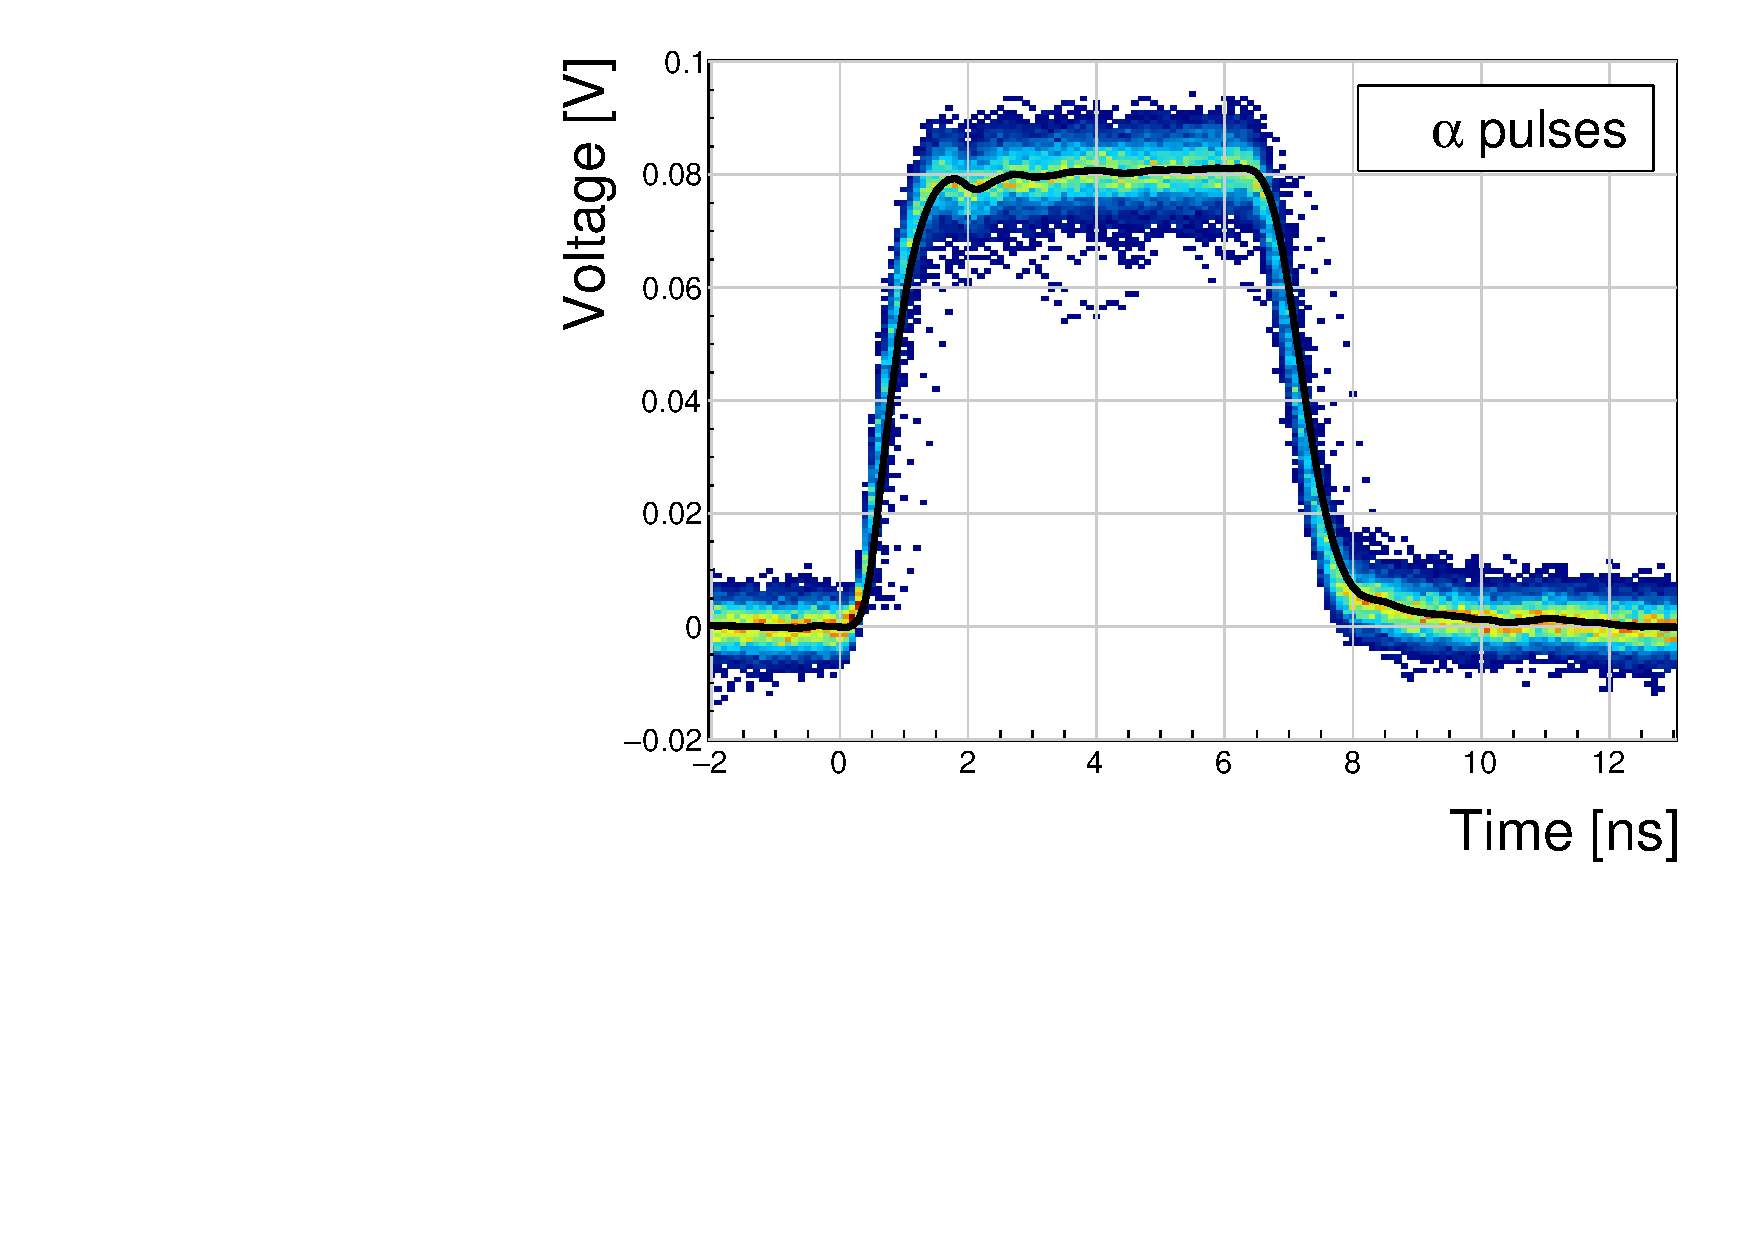
\includegraphics[width=0.30\textwidth]{scripts/plots/samplePulses/alpha} \label{fig:alpha1}} &
\subfloat[$\upbeta$ pulses]{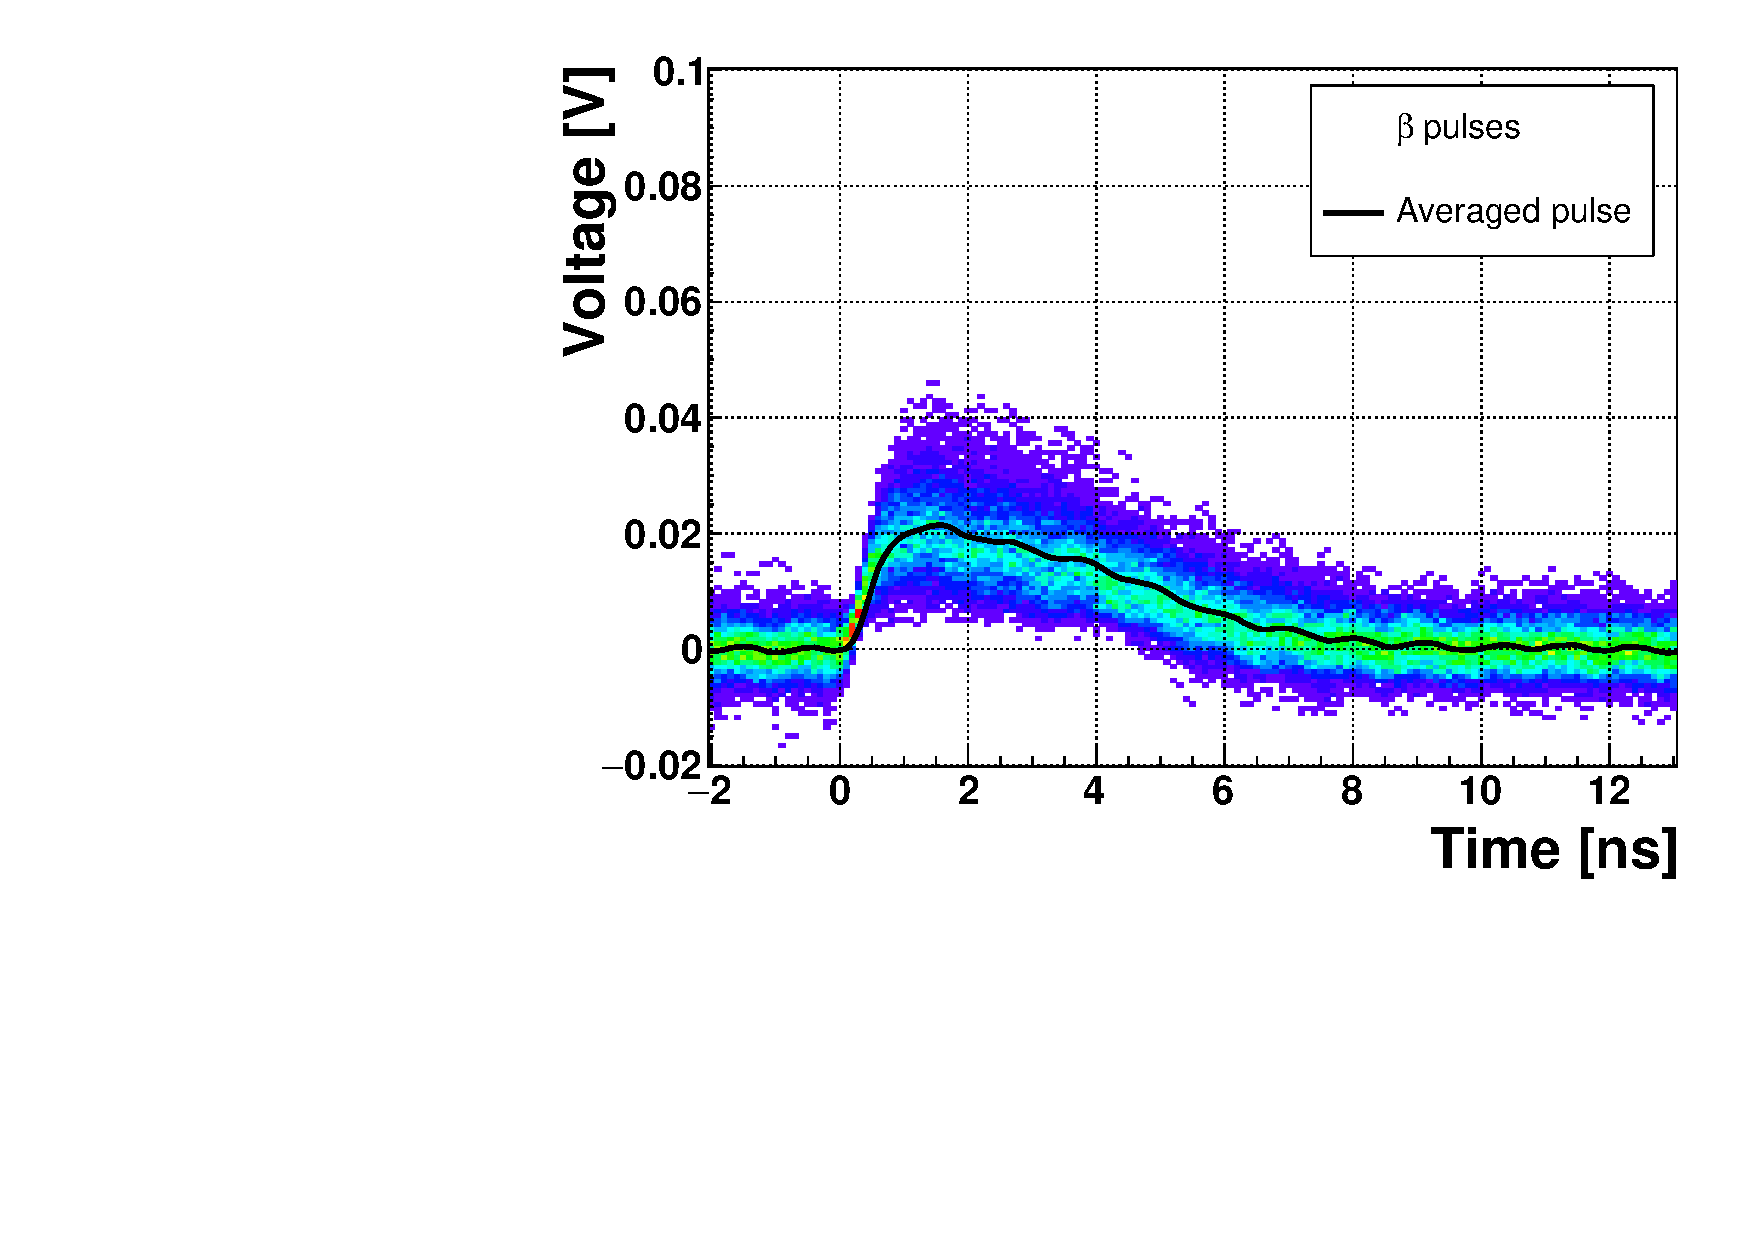
\includegraphics[width=0.30\textwidth]{scripts/plots/samplePulses/beta}  \label{fig:beta1}} &
\subfloat[$\upgamma$ pulses]{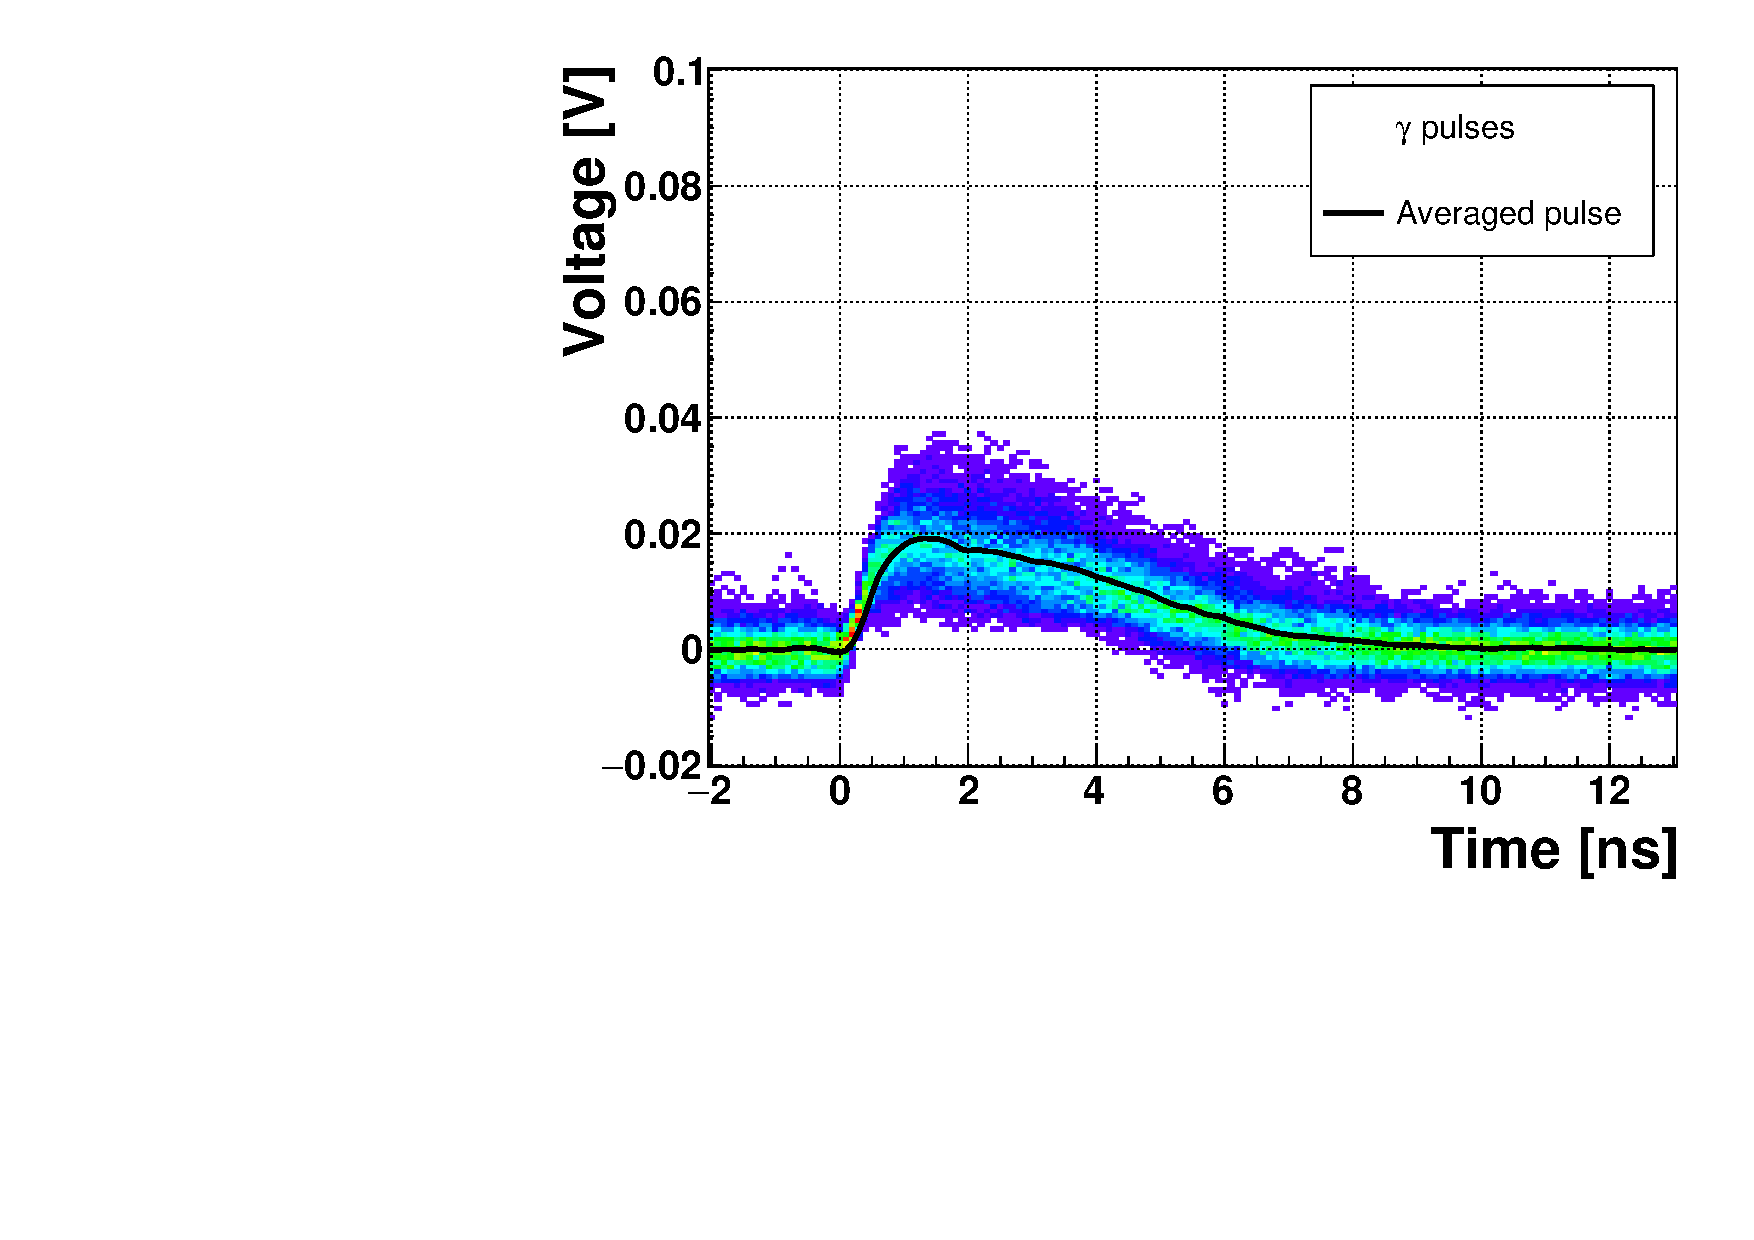
\includegraphics[width=0.30\textwidth]{scripts/plots/samplePulses/gamma}  \label{fig:gamma1}} \\
\subfloat[$\upalpha$ pulses]{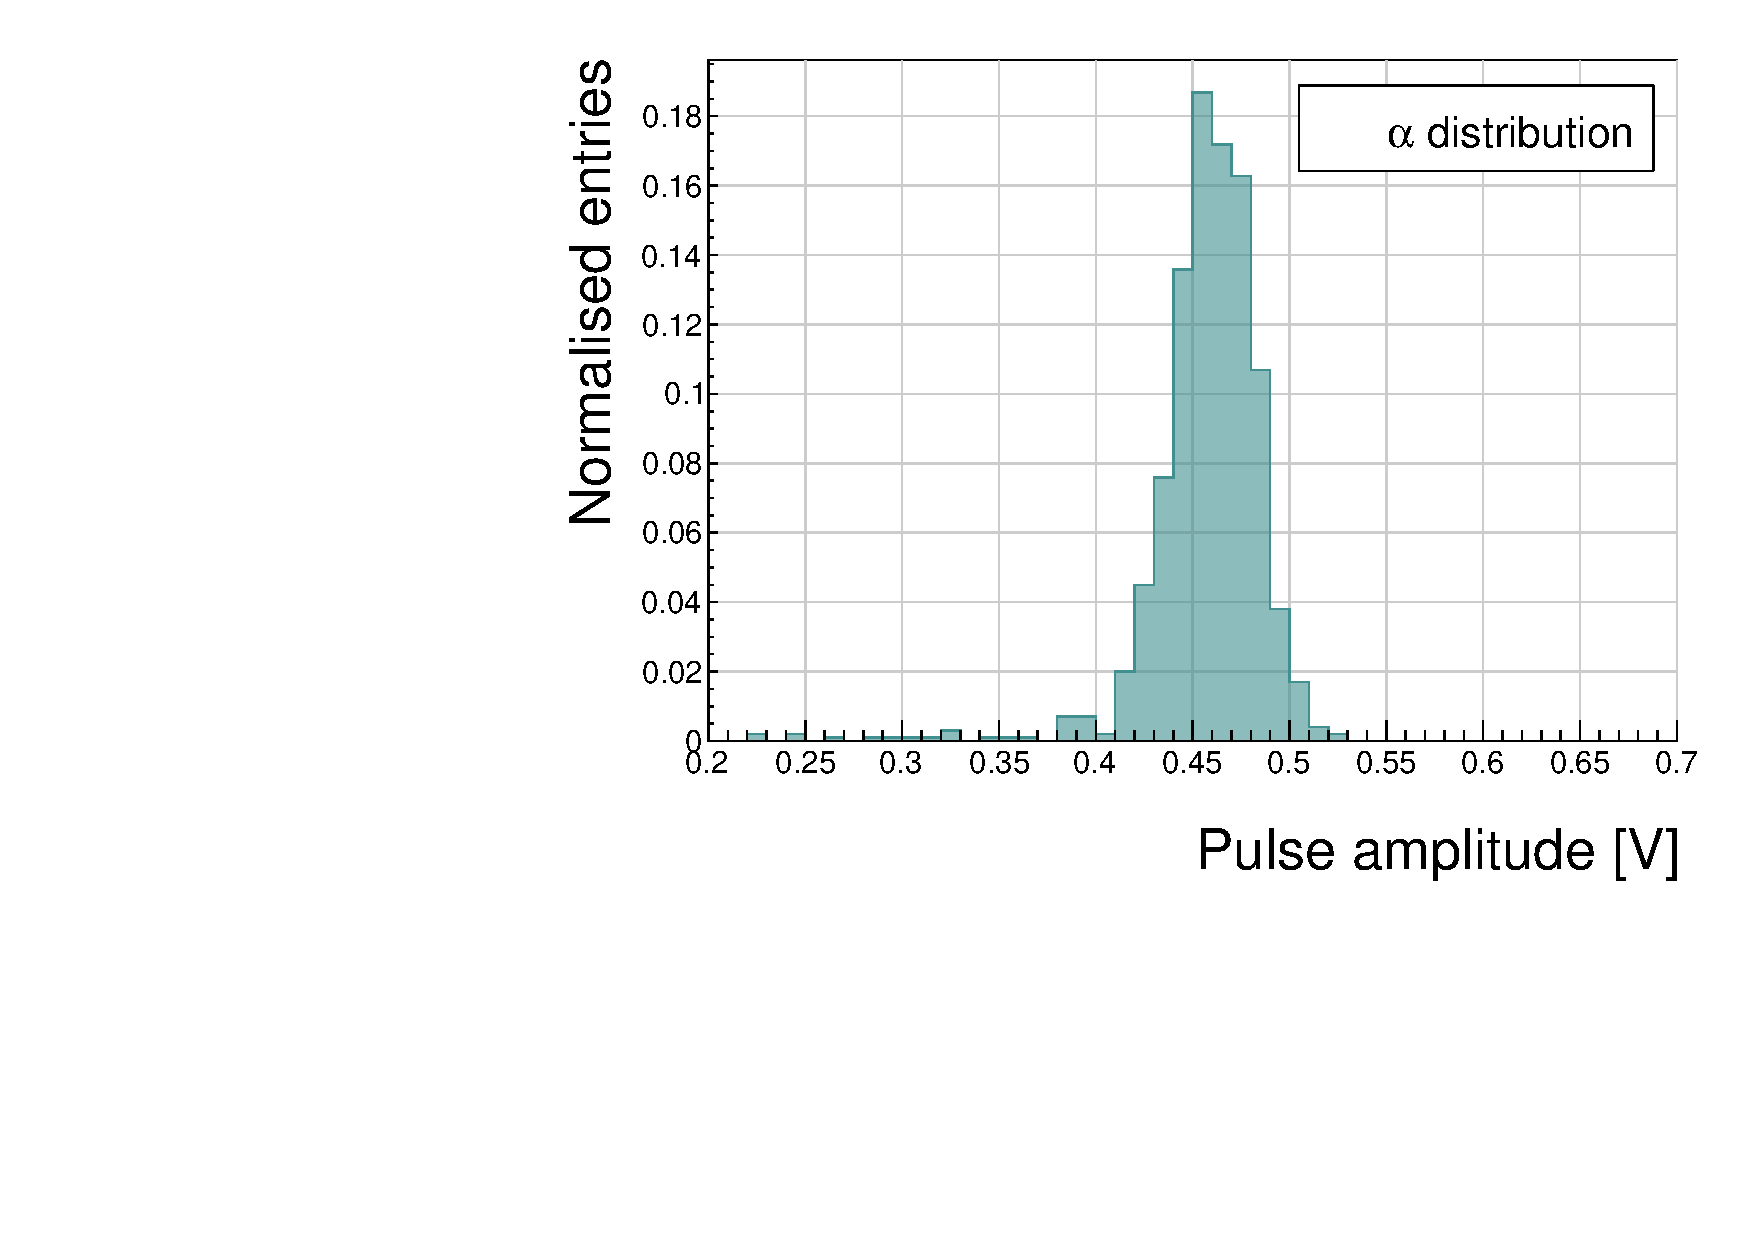
\includegraphics[width=0.30\textwidth]{scripts/plots/samplePulses/alphadist} \label{fig:alphadist1}} &
\subfloat[$\upbeta$ pulses]{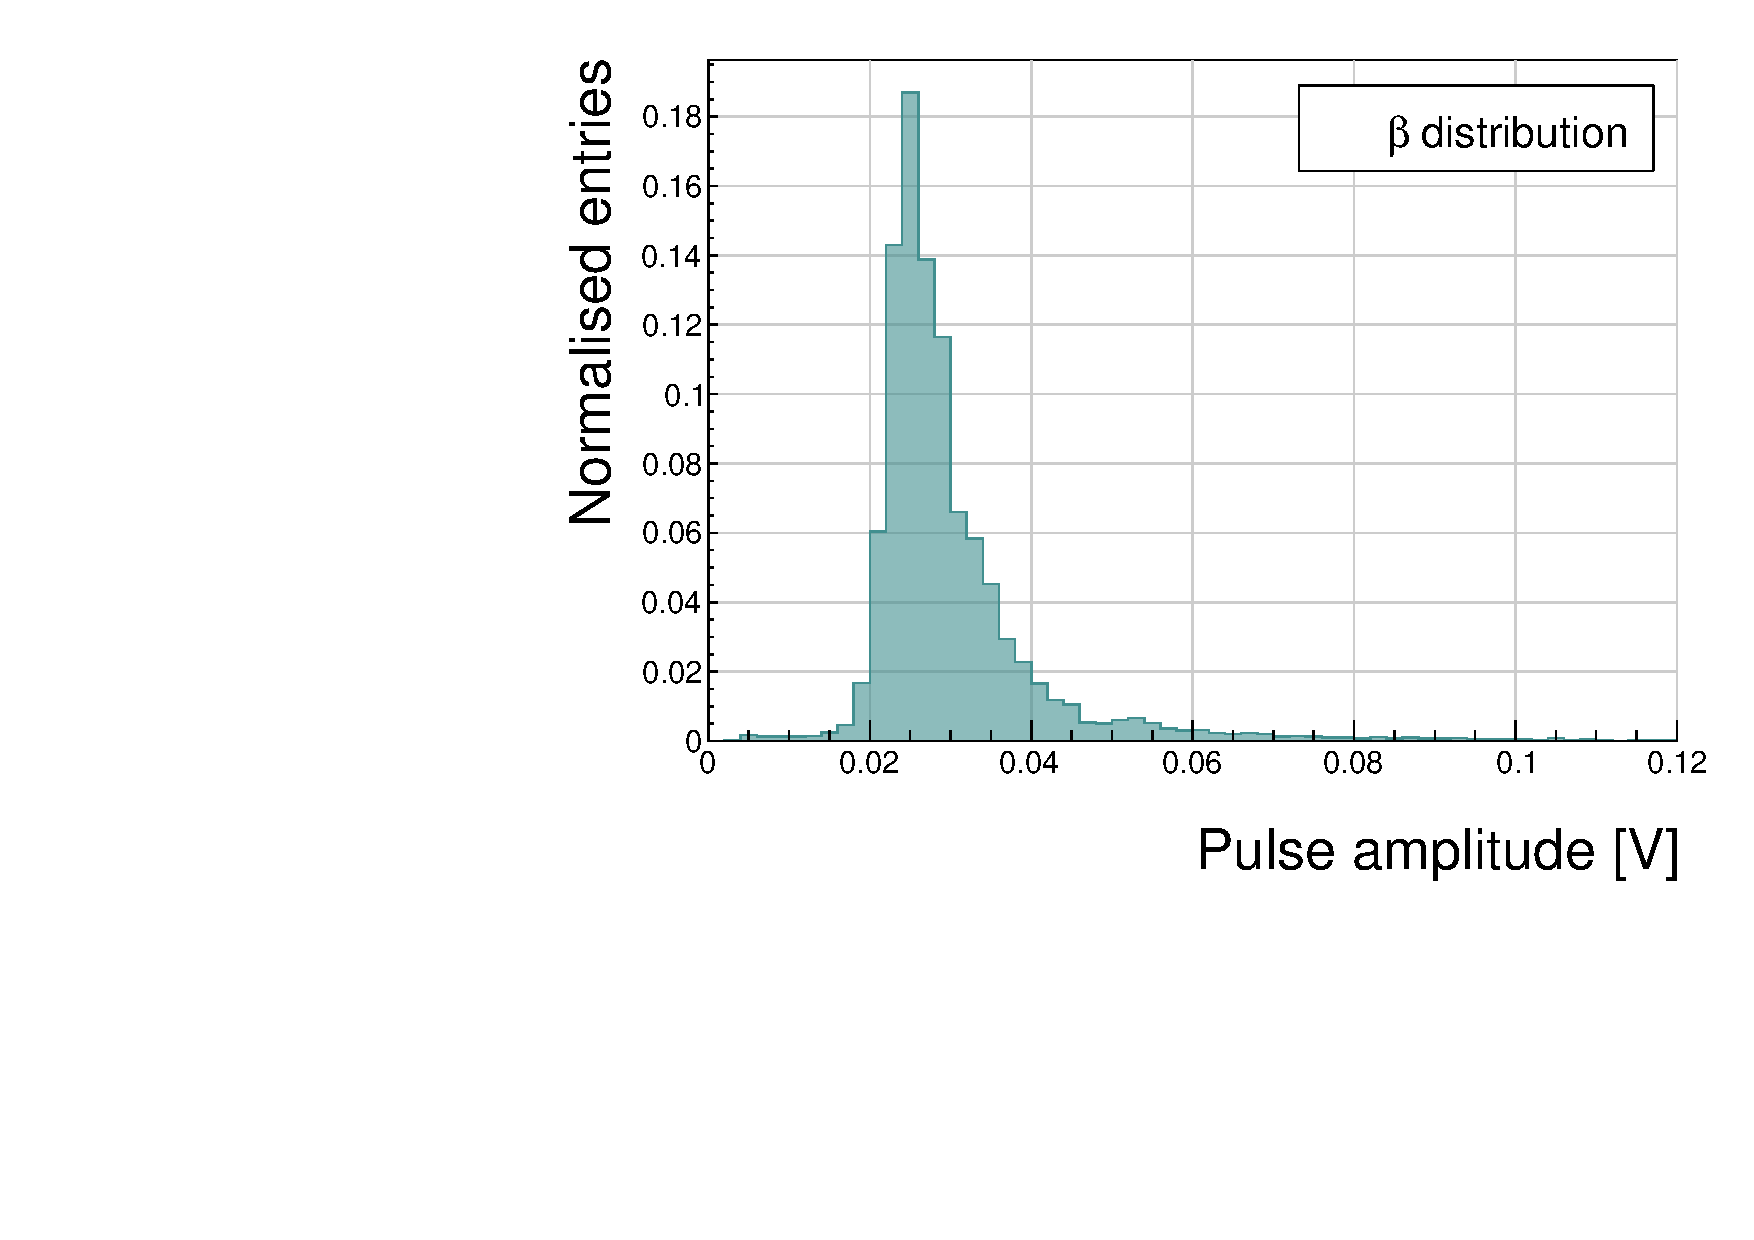
\includegraphics[width=0.30\textwidth]{scripts/plots/samplePulses/betadist}  \label{fig:betadist1}} &
\subfloat[$\upgamma$ pulses]{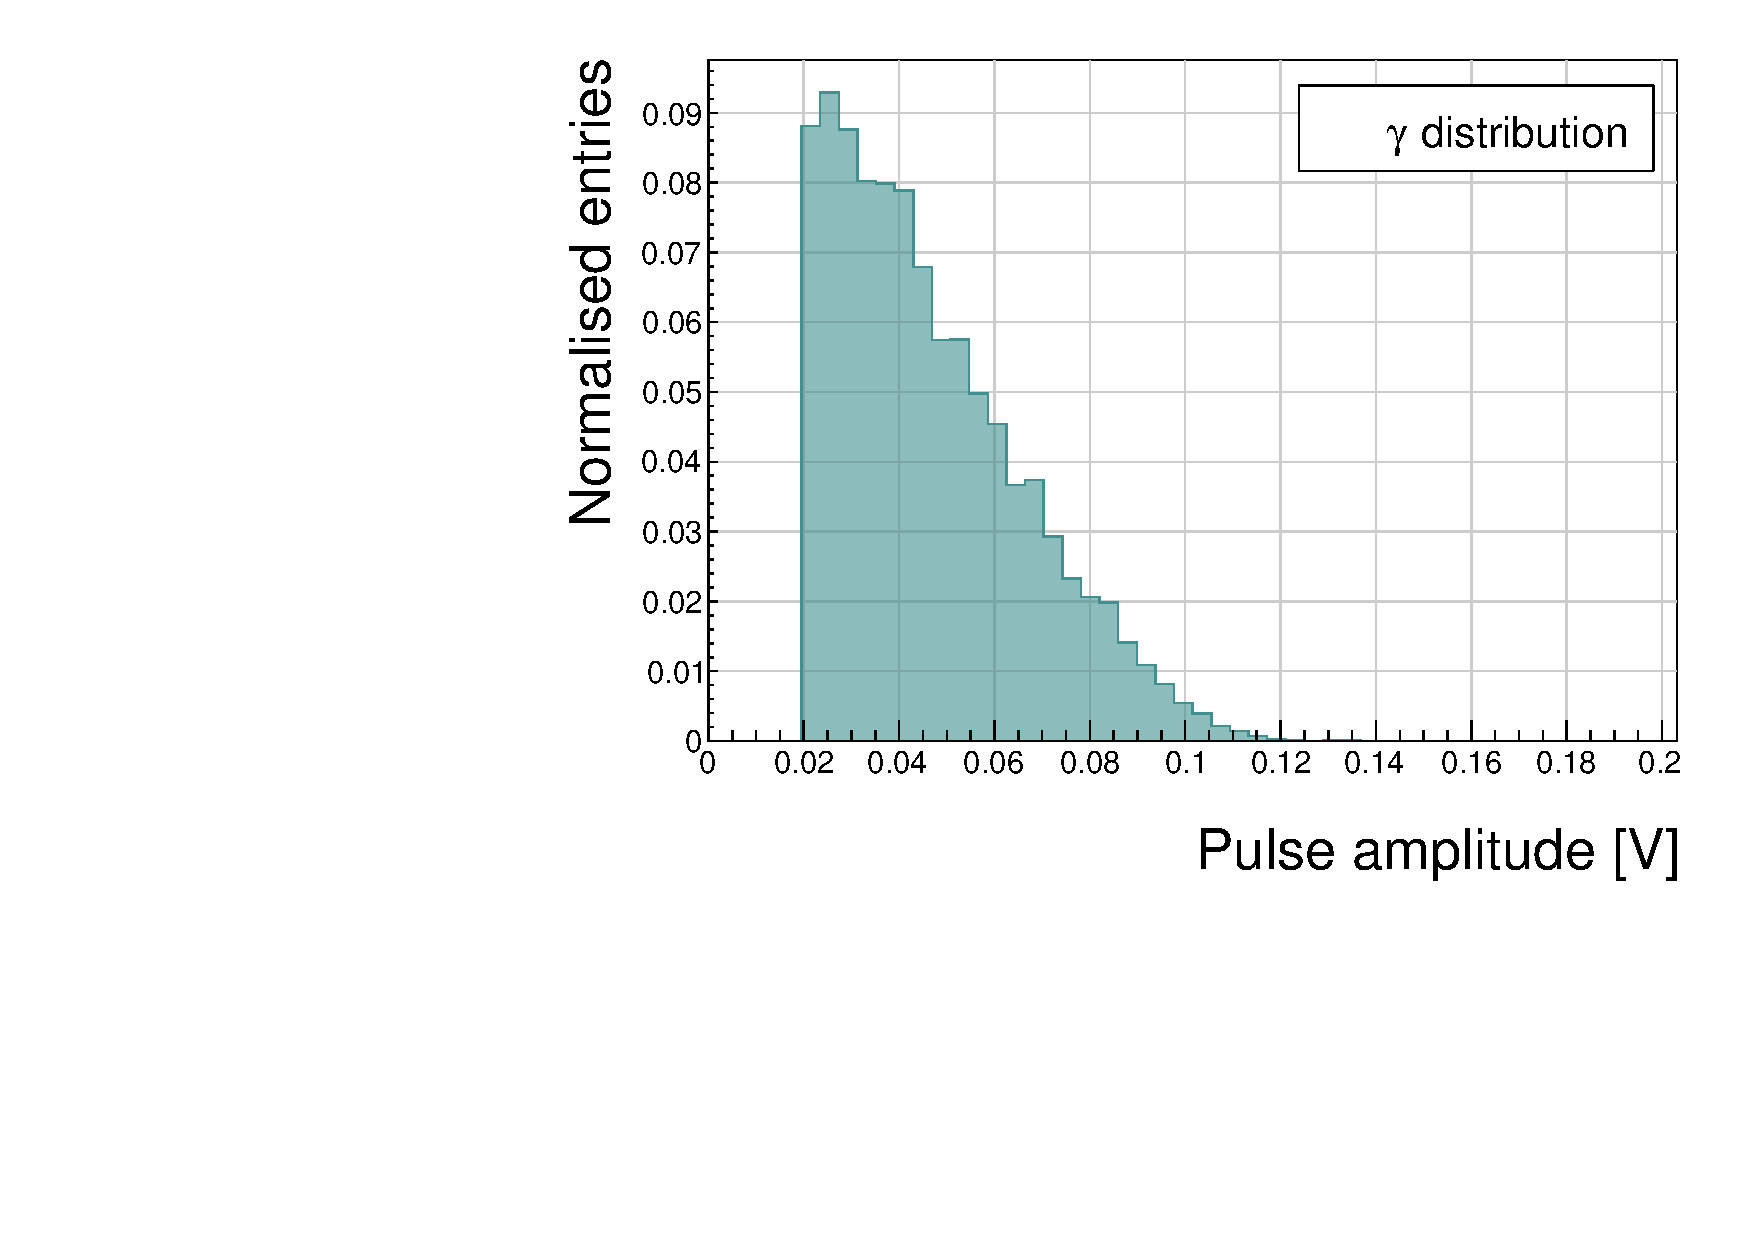
\includegraphics[width=0.30\textwidth]{scripts/plots/samplePulses/gammadist}  \label{fig:gammadist1}}
\end{tabular}
\caption{Superimposed and averaged pulses (a, b and c, current amplifier) and distributions of deposited energy (d, e, f, charge amplifier) for three types of radiation. Note the scale on the X axis of the distributions.}
\label{fig:pulsesaby}
\end{figure}




%---------------------------------------------------------------------------------------------------------------
%%\clearpage
\subsection{Noise limitations}
\label{sec:noiselimit}
%---------------------------------------------------------------------------------------------------------------
%TO DO: Take 8 runs with the 2GHz oscilloscope while increasing the noise. 
%TO DO: leakage current, irradiated.
Noise is a major limiting factor in particle detection. It defines the minimum measurable particle energy and the minimum measurement resolution. It is hence important to minimise the electric noise in the detector signal. The major noise contribution comes from poor shielding from external electromagnetic sources. These often cause ringing, whereby the signal oscillates with a frequency defined by the external source. The ringing makes high-frequency measurements impossible. Another source of noise is the sensor itself. In the case of silicon, natural light increases the number of thermally excited free charge carriers, increasing the leakage current. This is not the case for diamond, which is with its high energy band gap insensitive to visible light. Nevertheless, any noise produced by the sensors is amplified by the signal amplifiers, which add an additional noise of the analogue electrical circuit to the amplified signal. Finally, the digitisers add the quantisation noise to the digitised signal. If the measurement range is significantly higher than the actual measured signal, the quantisation noise can be a significant contributor to the decrease of the overall measurement resolution.






% ---------------------------------------------------------------------------------------------------------------
%\clearpage
\section{Radiation limitations}
\label{sec:radlimit}
% ---------------------------------------------------------------------------------------------------------------
Exposure to ionising radiation degrades sensors. It introduces charge traps by damaging the sensor material. The electrons and holes created by the impinging particle get trapped in these traps, decreasing the induced current on the electrodes. This yields a lower integrated charge in an irradiated sensor than that in a non-irradiated one. Charge collection efficiency is therefore correlated with the level of irradiation. This section contains a study of the effects of pion ($\uppi_{\mathrm{300~MeV}}$) irradiation on the charge collection efficiency of sCVD diamond detectors. To carry out this study, two diamond samples were irradiated to doses of 1$\times10^{14}~\pi$~cm$^{-2}$ (S79) and to 3.63$\times10^{14}~\pi$~cm$^{-2}$ (S52). Then a test beam campaign was carried out to observe the charge collection efficiency at different bias voltage settings. The highest achieved efficiency values were used to determine the effective drop in efficiency with respect to received radiation dose. A model~\cite{} defined by a collaboration researching diamond behaviour RD42 was applied to the measured values and a damage factor was extracted. The next subsection contains measurements and results of a long-term stability study using $\upalpha$ and $\upbeta$ particles. In particular, the charge collection efficiency as a function of time was measured during the measurements with $\upbeta$ and $\upalpha$ radiation. To investigate this effect on the scale of charge carriers, the change of TCT pulses with time was observed. Finally, a procedure that improves the pulse shape and with it the charge collection is proposed.

\subsection{Quantifying radiation damage in diamonds}
Radiation damage varies with the type of radiation (particles or photons) and its energy. There are several models existing~\cite{, , } that try to explain the impact of irradiation and to provide \emph{hardness factors} to compare the radiation damage between different particles. The standard way is to convert the damage into \emph{neutron equivalent}~\cite{}. Some models have been extensively verified with simulations and with experiments. In these experiments charge collection in sensors is measured before and after irradiation. This procedure is repeated several times, with a measurement point taken after every irradiation. When a set of measurements of charge collection is plotted against the radiation dose received by a specific particle at a specific energy, a damage factor $k_\mathrm{\lambda}$ can be extracted. Damage factors have to be measured across a range of energies and types of radiation to properly quantify the damage in the sensors~\cite{}. They are then compared against the simulations to verify that the experimental observations are in line with the theory.

Diamond is an expensive material and the technology is relatively new as compared to silicon. Therefore not many institutes are carrying out diamond irradiation studies. To join the efforts, the RD42 collaboration~\cite{} was formed. It gathers the experimental data from diamond irradiation studies. Unlike with silicon, the experimental results so far show no significant correlation with the NIEL (non-ionising energy loss) model~\cite{XXX}, which correlates detector efficiency with the \emph{number of lattice displacements}. Therefore an alternative model was proposed~\cite{XXX}, correlating the diamond efficiency with \emph{displacements per atom} (DPA) in the bulk. Figure~\ref{fig:kitdpa} shows the DPA model for a range of energies of proton, pion and neutron irradiation in diamond. According to the figure, a 300~MeV pion beam damages the diamond bulk twice as much as a 24~GeV proton beam. The data points obtained by RD42 are also added to the figure. They have been normalised to damage by 24~GeV protons. Finally, the data point measured in the scope of this thesis has been added for comparison. The calculation is done below.


\begin{figure}[!t]
\begin{center}
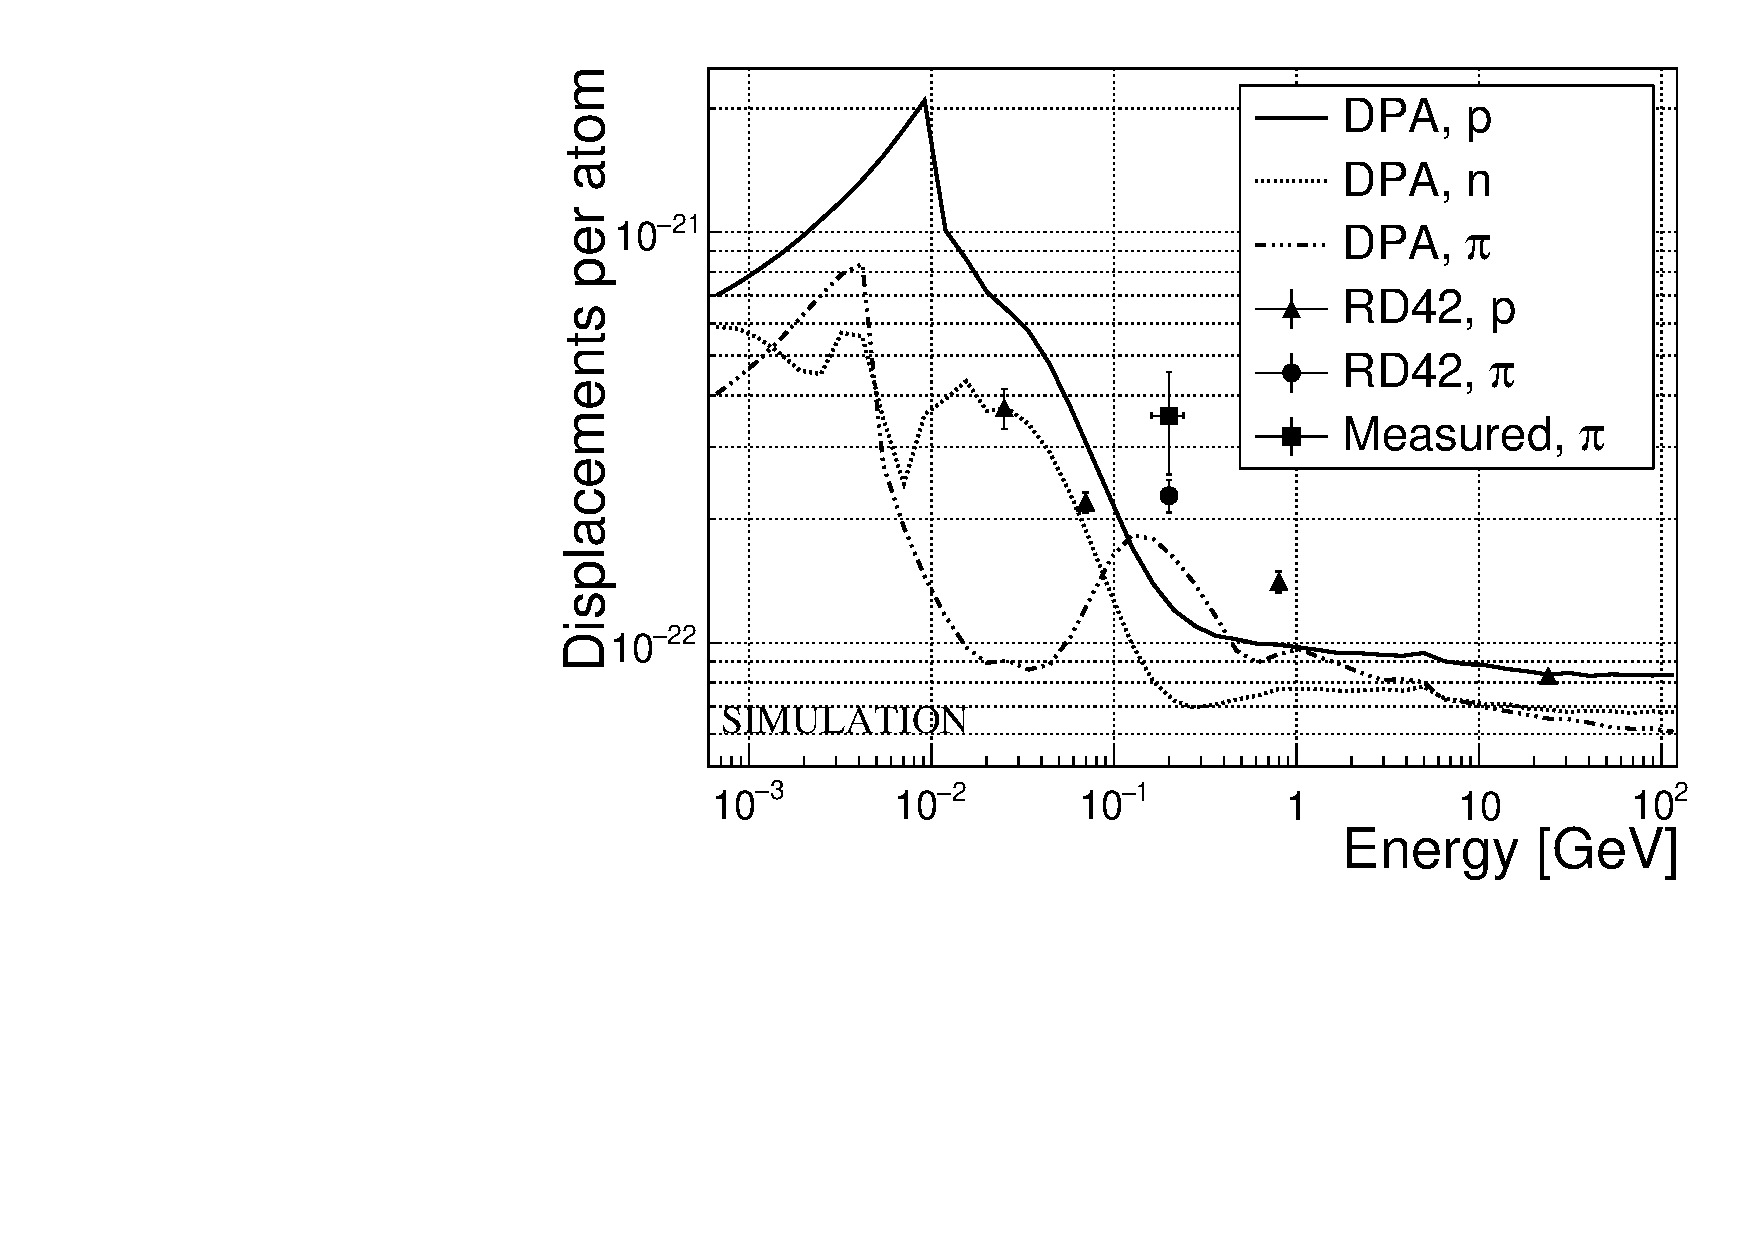
\includegraphics[width=0.7\textwidth]{scripts/plots/dpa1}
\caption{Diamond radiation damage - a model based on displacements per atom~\cite{}. Added are data points for protons and pions by RD42~\cite{} and one data point for pions measured in the scope of this thesis.}
\label{fig:kitdpa}
\end{center}
\end{figure}



\subsubsection{Irradiation with a $\uppi_\mathrm{300~MeV}$  beam}
The samples were irradiated at the Paul Scherrer Institute (PSI)~\cite{} by means of a beam of pions with an energy of 300~MeV (kinetic energy 191.31~MeV) and with a flux of up to $1.5\times10^{14}~\pi$~cm$^{-2}$ per day. The system has a 10~\% uncertainty on the beam energy. In addition, the equivalent fluence~\cite{} calculation has an error of $\pm20~\%$. Looking at the pion damage curve in figure~\ref{fig:kitdpa}, $\pi_{\mathrm{300~MeV}}$ point sits on a steep section of the DPA curve. This means that a deviation in beam energy can have a significant effect on the damage.
%After fitting a linear function between, the error on the DPA due to the uncertainty on the beam energy amounts to 7~\%. Overall error on the fluency is therefore the root mean square of the uncertainty on the DPA and the uncertainty on the hardness factor: $\upsigma=21~\%$.

Two diamond samples, S52 and S79, were put in the $\uppi_\mathrm{300~MeV}$ beam in the 2014 PSI irradiation campaign; S52 to $(1\pm0.21)\times10^{14}~\pi$~cm$^{-2}$ and S79 to $(3.63\pm0.77)\times10^{14}~\pi$~cm$^{-2}$. During the process, the golden electrodes got slightly activated, but the activation decayed in two weeks.

\subsubsection{Charge collection efficiency and charge collection distance}
Three diamonds -- non-irradiated S37 and irradiated S52 and S79 -- were tested in a $\uppi_\mathrm{120~GeV}$ test beam~\cite{} before and after irradiation. The goal was to estimate the charge collection efficiency (CCE) and charge collection distance (CCD) as a function of irradiation dose. The samples were primed (pumped) prior to data taking using a $^{90}$Sr radioactive source. The data were then taken at a range of bias voltages ranging from 30~V to 900~V, yielding between 0.06~V/$\upmu$m and 1.8~V/$\upmu$m electrical field in the bulk. Every data point contained approximately $5\times10^4$ measured particles. The charge deposited by the particles was measured using a CIVIDEC Cx charge preamplifier. As expected, the integrated amplitude spectrum followed a landau distribution.
%, as seen in figure~\ref{fig:landausample}. 
Its most probable value (MPV) was used to calculate the most probable collected charge $Q_\mathrm{i}$:
\begin{equation}
\label{eq:ccdcalc}
Q_\mathrm{i}~[e^-] = \frac{ Q_i~[fC] } { 1.6\times 10^{-4} }= \frac{MPV~[mV]}{A~[mV/fC]} \cdot 6.241\times 10^{4}
\end{equation} 
where A$=9.2$~mV/fC is the preamplifier gain factor. The CCD was then calculated using the average number of electron-hole pairs produced per micrometer in diamond $\delta_d = 36~$e-h~$\upmu$m$^{-1}$ (from table~\ref{tab:semicompare}):
\begin{equation}
\label{eq:ccdcalc1}
CCD = \frac{Q_\mathrm{i}}{\delta_\mathrm{}d}
\end{equation} 

% sample landau distribution  
%\begin{figure}[!t]
%\begin{center}
%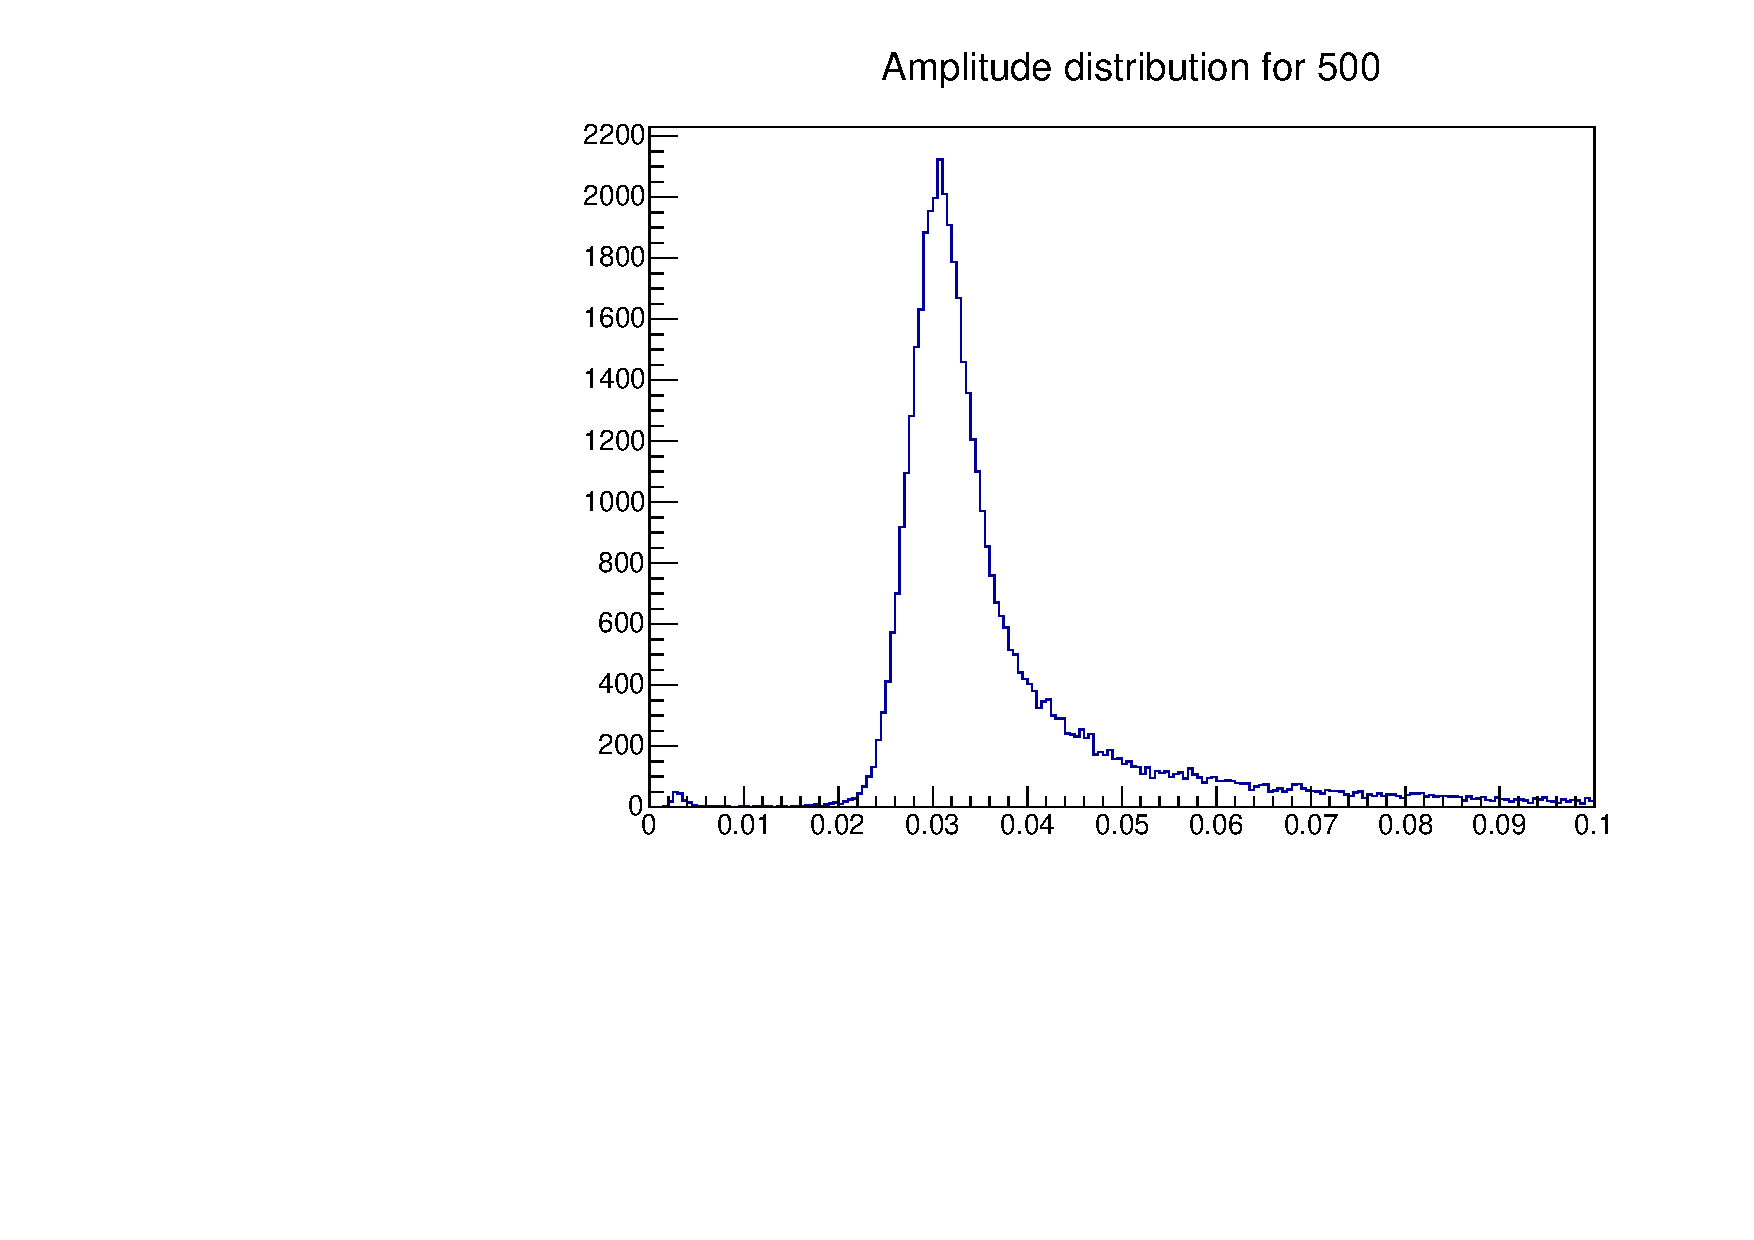
\includegraphics[width=0.6\textwidth]{scripts/pics/S37_500}
%\caption{An example of a landau distribution acquired by S37 at 500~V bias voltage PLACEHOLDER}
%\label{fig:landausample}
%\end{center}
%\end{figure}
The resulting CCD for the three measured samples at bias voltages ranging from 0.2--1.6~V~$\upmu$m$^{-1}$ is shown in figure~\ref{fig:ccd}. S37 exhibits full collection distance already at 0.4~V~$\upmu$m$^{-1}$ whereas the irradiated samples have a more gentle increase of CCD with increasing bias voltage. It is evident that at 1~V~$\upmu$m$^{-1}$  the maximum CCD has not been reached in the case of S79 and S52.

% CCD against HV 
\begin{figure}[!t]
\centering
\begin{tabular}{cccc}
\subfloat[CCD for S37, S79 and S52]{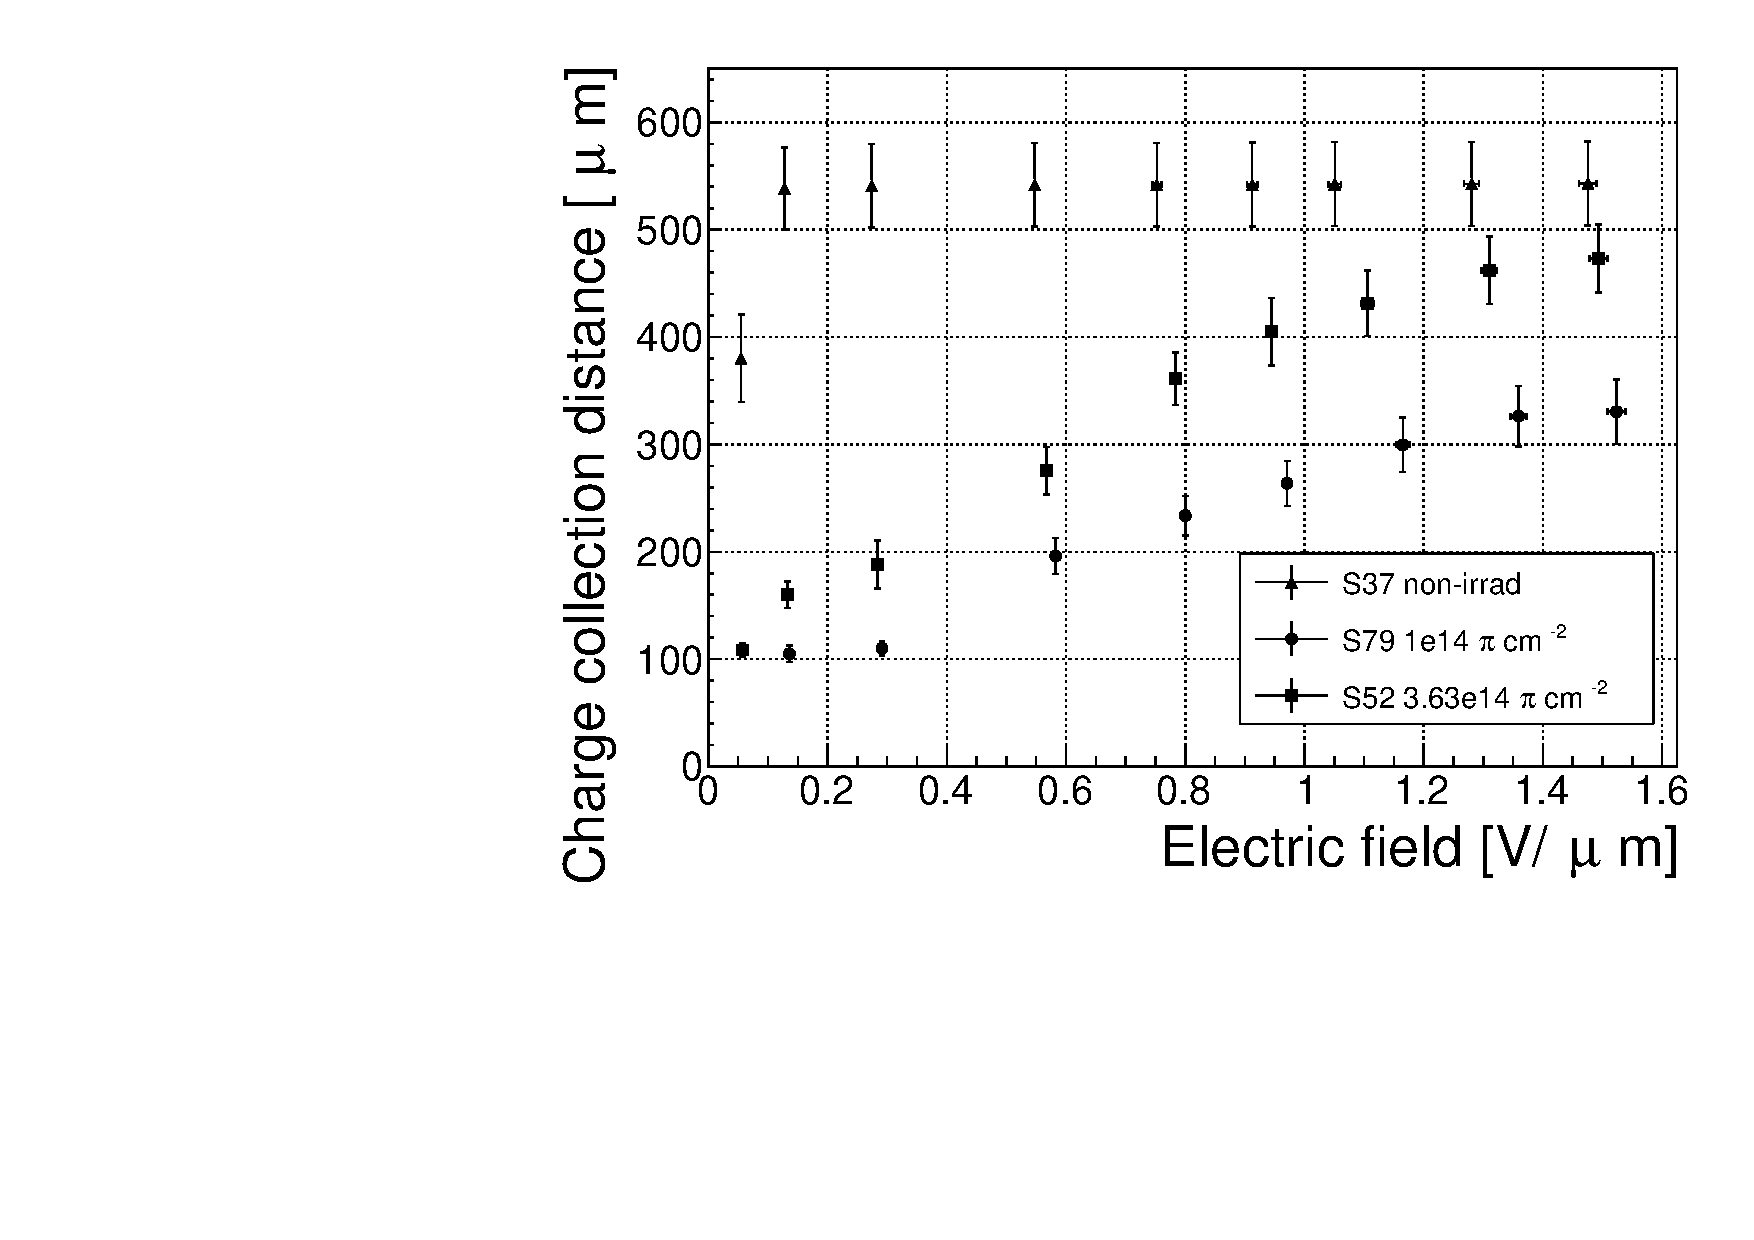
\includegraphics[width=0.80\textwidth]{scripts/plots/ccd} \label{fig:ccd}} \\
\subfloat[Comparing the data points obtained in a test beam against the RD42 data]{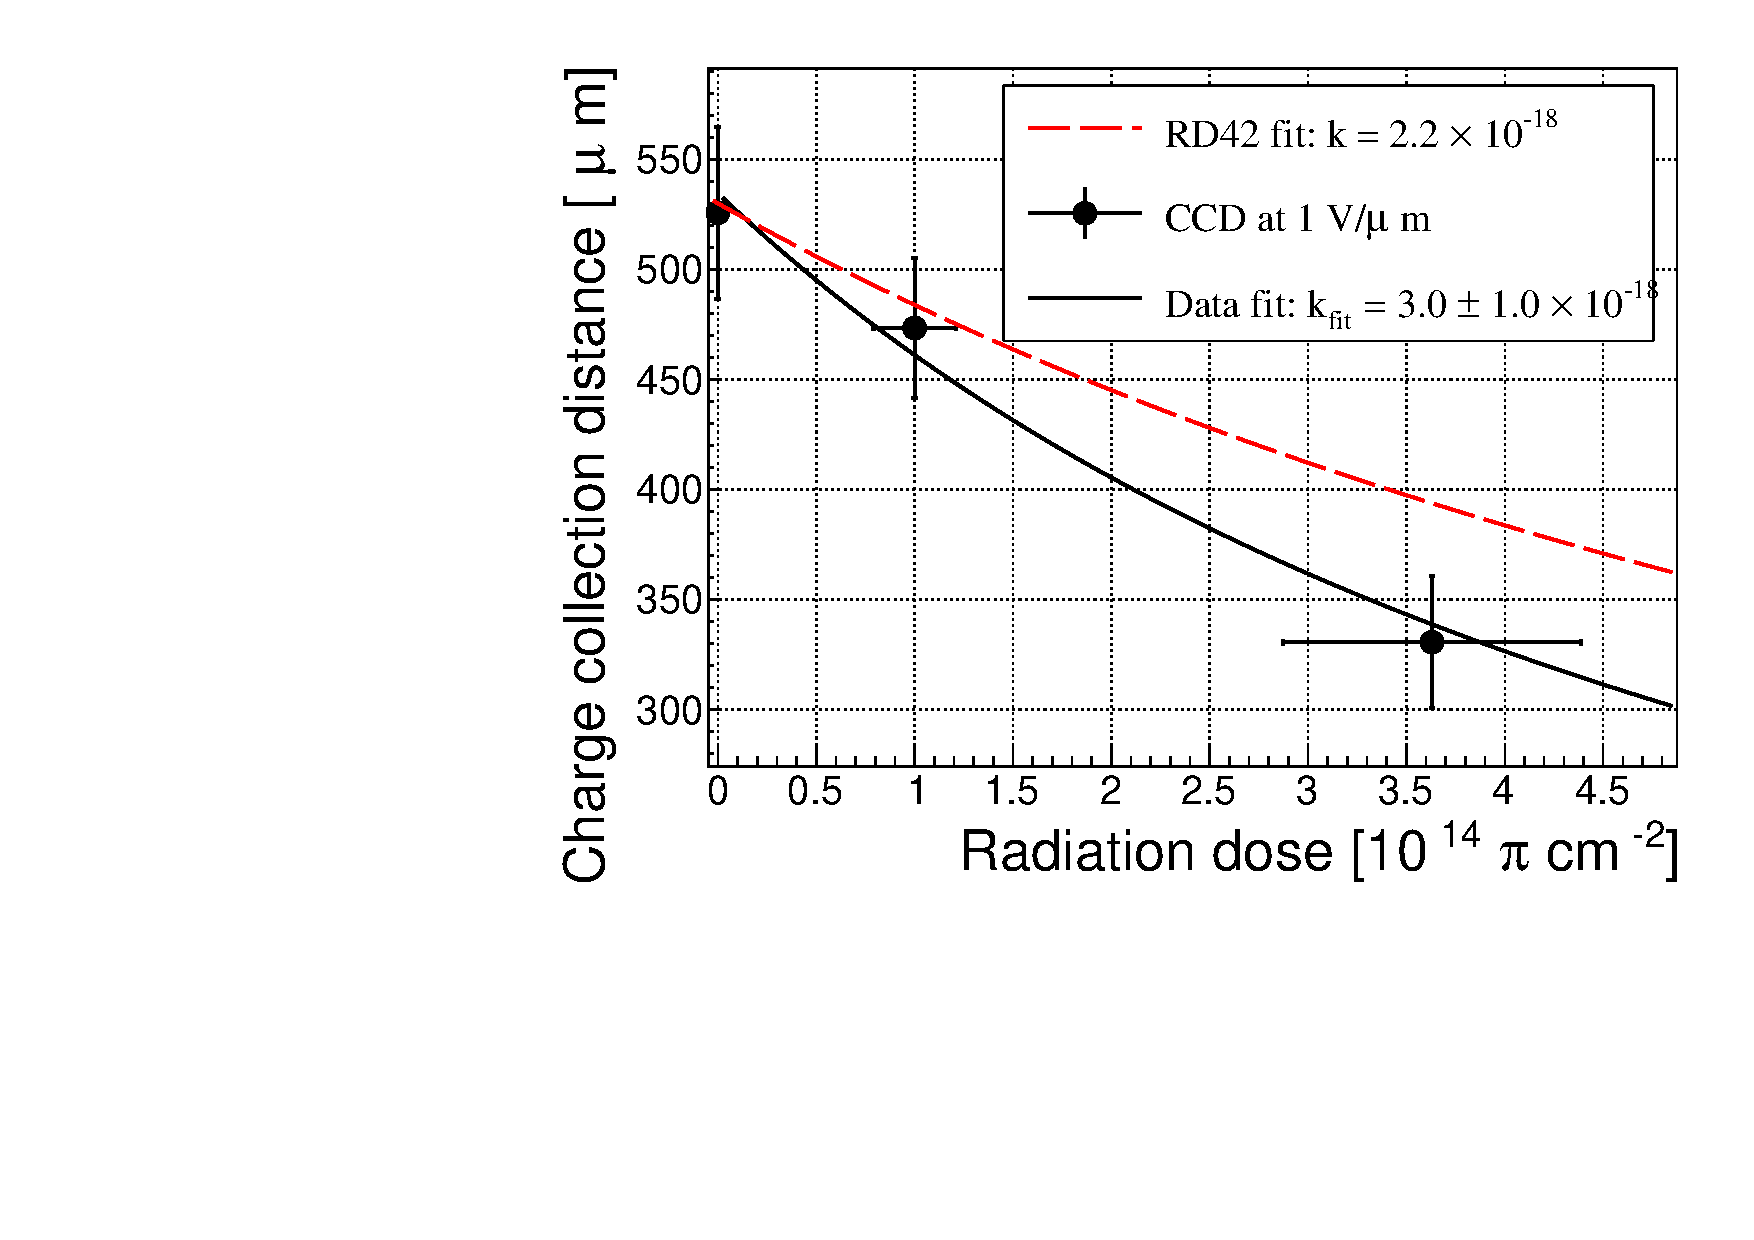
\includegraphics[width=0.80\textwidth]{scripts/plots/radfactor}  \label{fig:radfactor}}
\end{tabular}
\caption{The charge collection distance at 500~V bias voltage for the three diamond samples was compared to the RD42 data for pion irradiation. The data points are about 5--15~\% lower than expected from the RD42 data~\cite{}.}
\end{figure}

\subsubsection{Irradiation damage factor}
The irradiation damage factor $k$ is a way to quantify irradiation damage of a specific particle at a specific energy. Via this factor different types of irradiation can be compared. It is obtained experimentally by measuring the CCD of a number of samples at various irradiation steps and fitting the equation~\ref{eq:radfactor1} to the data. $\lambda$ is the measured CCD, $\lambda_\mathrm{0}$ is the CCD of a non-irradiated sample and $\Phi$ the radiation dose.


\begin{equation}
\label{eq:radfactor}
\frac{1}{\lambda} = \frac{1}{\lambda_\mathrm{0}}+k_{\lambda}\cdot\Phi
\end{equation} 
\begin{equation}
\label{eq:radfactor1}
\lambda = \frac{\lambda_\mathrm{0}}{k_{\lambda} \lambda_0 \Phi + 1}
\end{equation} 

The data points with the maximum CCD obtained in the test beam measurements are plotted against radiation dose received (see figure~\ref{fig:radfactor}). Equation~\ref{eq:radfactor1} is fitted to the data points and a damage factor $k_{\mathrm{\lambda}}=(3.0\pm1.0)\times10^{-18}~\upmu$m$^{-1}$~cm~$^{-2}$ was obtained. This value is for a factor of two higher than the damage factor obtained by RD42. %The irradiated samples do not yet have a full charge collection at 1.0~V~$\upmu$m$^{-1}$. 
Also, with only two samples measured, the statistical uncertainty is high. Nevertheless, it can be concluded that the 300~MeV pions damage the diamond bulk more than the 24~GeV protons.




\subsection{Long-term measurement stability}
An important requirement for particle detectors is a stable performance over long periods of time. For instance, the charge collection for a defined radiation type and quantity must not change over time or has to change in a predicted way. Diamonds are stable as long as their environment and their operating point does not change significantly. The stability of diamond detectors depends on many factors (material purity, polishing process, electrode material, irradiation damage etc.). The aim is to study the behaviour of diamond under controlled conditions, with the goal to understand its limitations. One of these limitations is for sure the received radiation dose as it can affect the long-term stability of the sensor during operation. 

The three diamond samples (S37, S79 and S52) have been exposed to two different types of ionising radiation for a longer period to see if their behaviour changes over time. Two parameters have been observed in particular: 
\begin{enumerate}
\item Charge collection of $\upbeta$ particles and 
\item Charge collection and ionisation profile of $\upalpha$ particles.
\end{enumerate}
The results in this and in the next section will show that, in both cases, priming plays an important role in improving the diamond measurement stability. 
%NOTE I can use this part for conclusion
%The $\upbeta$ particles have a ``healing'' effect on the diamond; MIP detection is therefore rather stable in the long run, despite the fact that the sensors had been degraded by means of irradiation. Alpha particles, on the other hand, deteriorate the measurement, probably by introducing space charge into the sensor bulk. 

\subsubsection{$\upbeta$ long-term stability}
The diamond samples have undergone a long-term stability test using $\upbeta$ radiation. This has been done using a $^{90}$Sr source emitting $\sim$2~MeV electrons at a rate of approximately $10^4$~e$^-$~cm$^{-2}$. To simulate the initial conditions in HEP experiments, the sensors must not be primed before starting the measurements. The measurement setup consists of a diamond sample (S37, S52 or S79) with the Cx spectroscopic amplifier, a silicon diode with a C6 amplifier for a trigger and a $^{90}$Sr source on top. A particle emitted by the source traverses the sensor bulk and hits the silicon diode, triggering the analogue signal readout. The source is left on the top for the course of the experiment. The measurements, however, are taken at discrete times. For every data point, approximately $10^4$ triggers are recorded. The offline analysis of the recorded signal pulse amplitudes yields a landau distribution for every data point. The most probable value (MPV) of the distribution is proportional to the collected charge by the diamond sensor. The resulting graph of charge collection over time (see figure~\ref{fig:ccincrease}) shows that the charge collection efficiency improves when the diamond sensor is primed with a $\upbeta$ source. This is especially evident in the case of the two irradiated samples. S79 achieves close to a full efficiency whereas S52 reaches about 50~\%. Both increases are significant. At a received dose of approximately 4$\times10^6$~particles the signal stabilises. As expected, the signal of the non-irradiated S37 does not change with time -- this pure sCVD diamond sample has the maximum collection distance from the start of the measurement.

It should be noted that the $\sim$2.28~MeV electrons emitted by this source are not MIPs; their charge deposition is higher than that of an electron MIP, according to the Bethe-Bloch distribution~\cite{}. Nevertheless, for the purpose of these measurements this energy was adequate since only the relative change in charge collection was of our interest.

To sum up, diamond is a good choice for $\upbeta$ radiation detection. Even if damaged by radiation, it reaches a stable charge collection at a received dose of $\sim$4$\times10^6$~MIP particles. The efficiency decreases with a high irradiation dose (effects visible above 10$^{12}$~MIP~cm$^{-2}$). However, the decrease can be accounted for if the damage factor and the rate and energy of the particles are known. $\upgamma$ radiation has a similar impact on the diamond as the $\upbeta$ because the ionisation mechanism is the same. The impinging photons, if they interact with the diamond, prime the bulk, causing the increase in charge collection efficiency. The difference, however, is that the interaction probability (cross section) is lower for gammas~\cite{}.

%%longterm pumping plot
\begin{figure}[!t]
\begin{center}
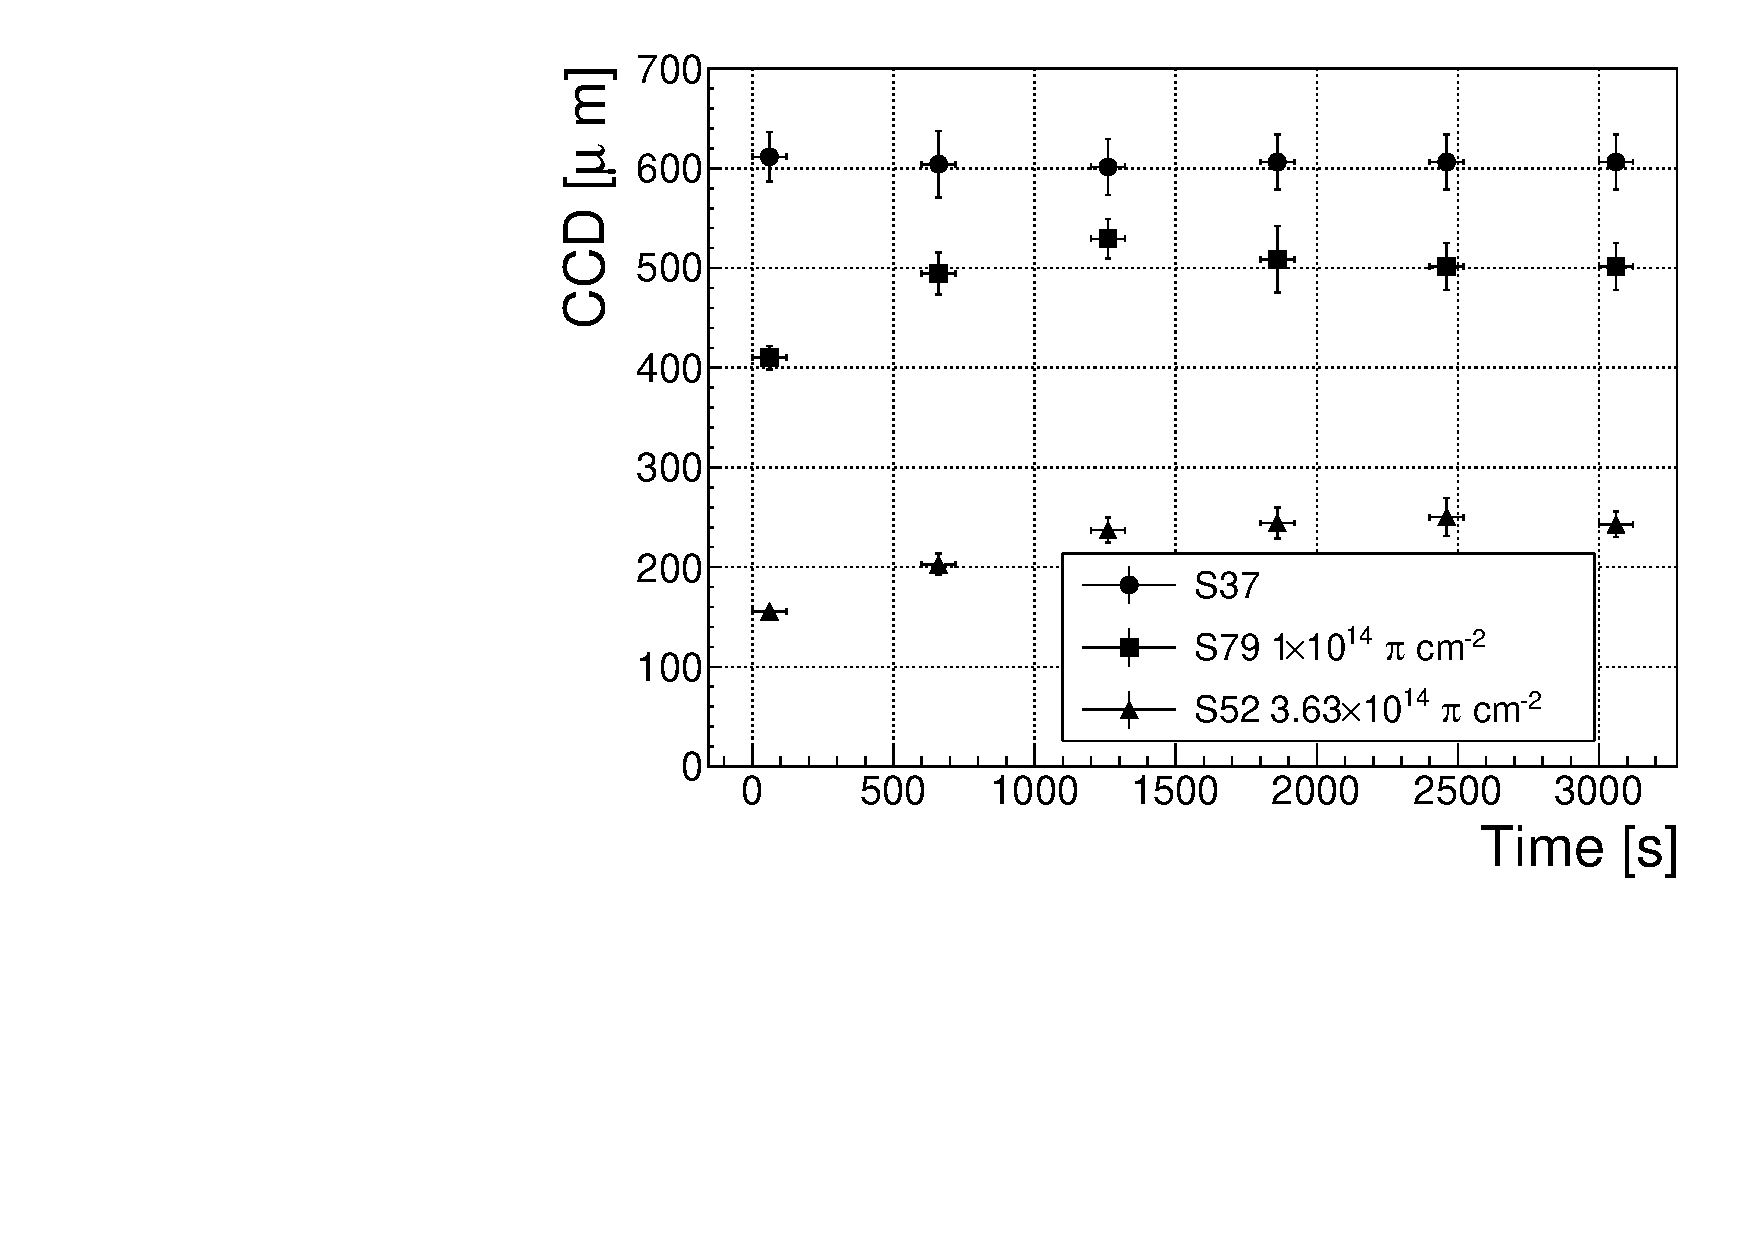
\includegraphics[width=0.6\textwidth]{plots/ccdpriming}
\caption{Increase of charge collection over time due to priming with the $^{90}$Sr radioactive source. The bias voltage for this measurement is 1~V/$\upmu$m.}
\label{fig:ccincrease}
\end{center}
\end{figure}


\subsubsection{$\upalpha$ long-term stability}
This part discusses the stability of irradiated diamond sensors during $\upalpha$ measurements. An $^{241}$Am source is used, emitting $\upalpha$ particles with a mean energy of 5.5~MeV. It is safe to assume that they will behave differently than when subject to $\beta$ radiation. This is due to the point-like charge carrier creation when an $\upalpha$ particle penetrates the bulk and stops at a depth of $\sim$14~$\upmu$m (for a 5.5~MeV particle). The deposited energy produces $\frac{5.5~MeV}{13.6~eV} = 4\times10^5$ e-h pairs. Compared to a MIP, which produces an MPV of $500~\upmu m~\times~36~e-h~\upmu m^{-1} = 18\times10^3$ e-h pairs in a 500~$\upmu$m, the collected charge is for a factor of 22 higher. In addition, the energy is deposited in a small volume -- 14~$\upmu$m in depth and $\sim$20~nm radially~\cite{}. This dense distribution of charge carriers affects their behaviour at the start of the drift. Furthermore, carriers of only one polarity drift through the sensor while those of the opposite polarity almost instantly recombine with the adjacent electrode. Taking into account that the diamond bulk has been damaged by irradiation, these two phenomena might have an effect on the operation of the detector on a macro scale.

%The measurement setup consisted of a PCB carrier for a diamond with a fitted $^{241}$Am source and a vacuum chamber. The carrier was placed into the chamber, which was then evacuated. t acted as shielding for external noise pickup and ensured that the $\upalpha$ particles didn't lose energy traveling through air. An SMA feedthrough ensured the electrical connection to the outside. The samples were measured before and after priming, at both polarities, to compare the behaviour of both electrons and holes as charge carriers. The scope of the measurements was to observe the changes in charge collection efficiency and/or in the pulse shapes. 

The first test has been carried out using the Cx spectroscopic amplifier, with the bias voltage of the samples set to +500~V. Figure~\ref{fig:longtermcx} shows the results of 6500 recorded hits at a rate of $\sim$7~particles per second. The collected charge for the non-irradiated sample is stable with time. It is expected that the irradiated samples will have a lower charge collection efficiency than the non-irradiated sample. However, their initial efficiency suddenly drops after a certain period of time. The initial efficiency is improved after priming with $\upbeta$ particles, but eventually it deteriorates again. In addition, the spread of measured energies increases significantly. Finally, the particle counting rate decreases with the decreased efficiency. 
\begin{figure}[!t]
\begin{center}
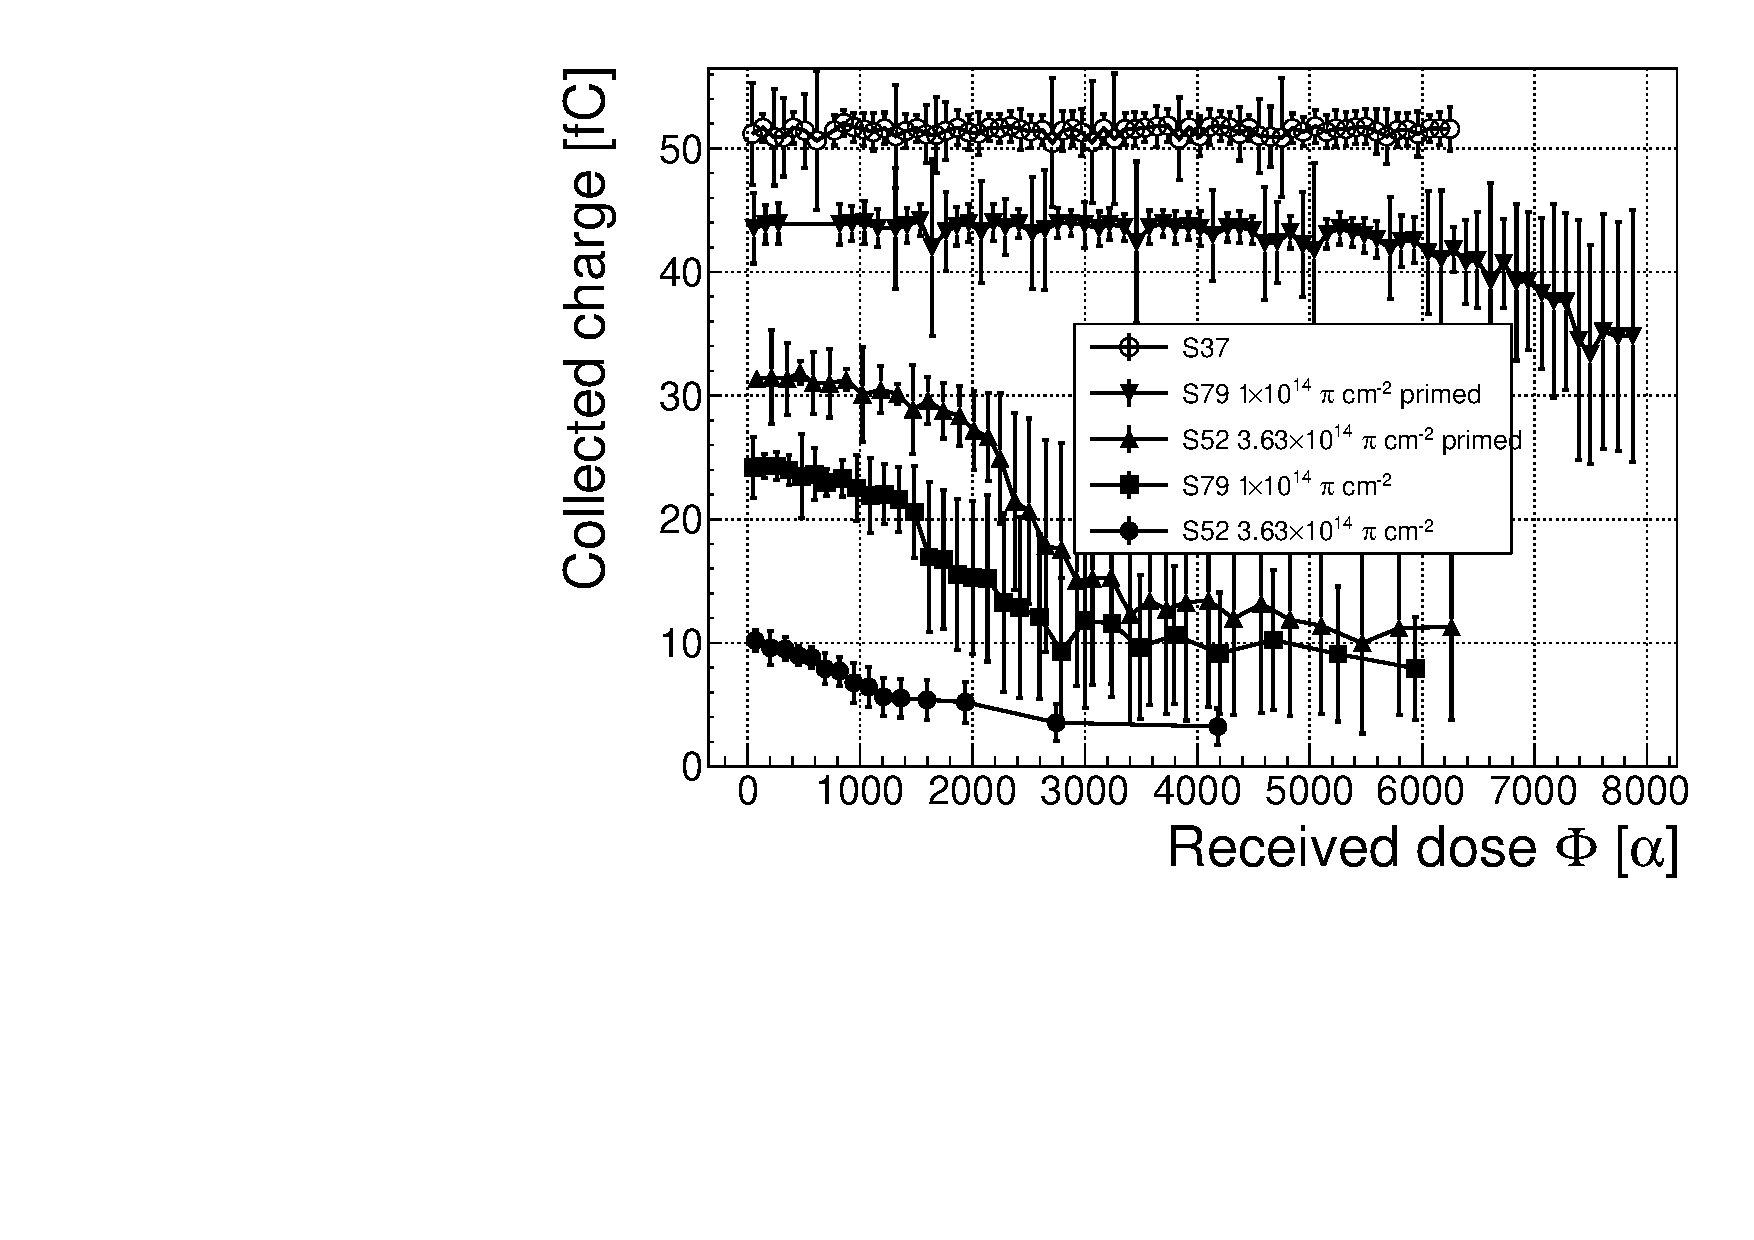
\includegraphics[width=0.8\textwidth]{scripts/plots/amplvstimecx}
\caption{Comparison of collected charge with time for non-irradiated and irradiated diamond samples.}
\label{fig:longtermcx}
\end{center}
\end{figure}

To investigate this sudden drop in efficiency, the current pulse shapes using a C2 current amplifier have to be observed (see figure~\ref{fig:lifetimeelecsholes}). The shape of the pulse holds more information about the charge carrier properties in the sensor than solely the value of the integrated charge. This time only the primed S79 sample has been tested. Both hole and electron collection are observed to determine whether they behave differently or not. The sample has been measured long enough for the pulse shapes to start changing. The data in figures~\ref{fig:lifetimeelecsholes} show that the initially stable pulses start deteriorating -- suddenly several different shapes start appearing, some still very similar to those from the beginning while the others with almost zero amplitude. 

Some charges get stopped in the charge traps in the bulk for a long time, building up regions of space charge. 
%DISCUSSION!!!
%Since only one charge flavour is drifting through the bulk whereas the other is quickly recombined, this already determines the imbalance in spatial distribution of trapped charges. 
The built up space charge affects the electric field, making it non-uniform. The non-uniform field in turn affects the drifting carriers, slowing them down or speeding them up, depending on the field gradient. Since the movement of the carriers is inducing  the electric current, the field gradient can be observed in the signal. 

\begin{figure}[!t]
%\centering
\begin{tabular}{rrr}
\subfloat[Holes at 0 min]{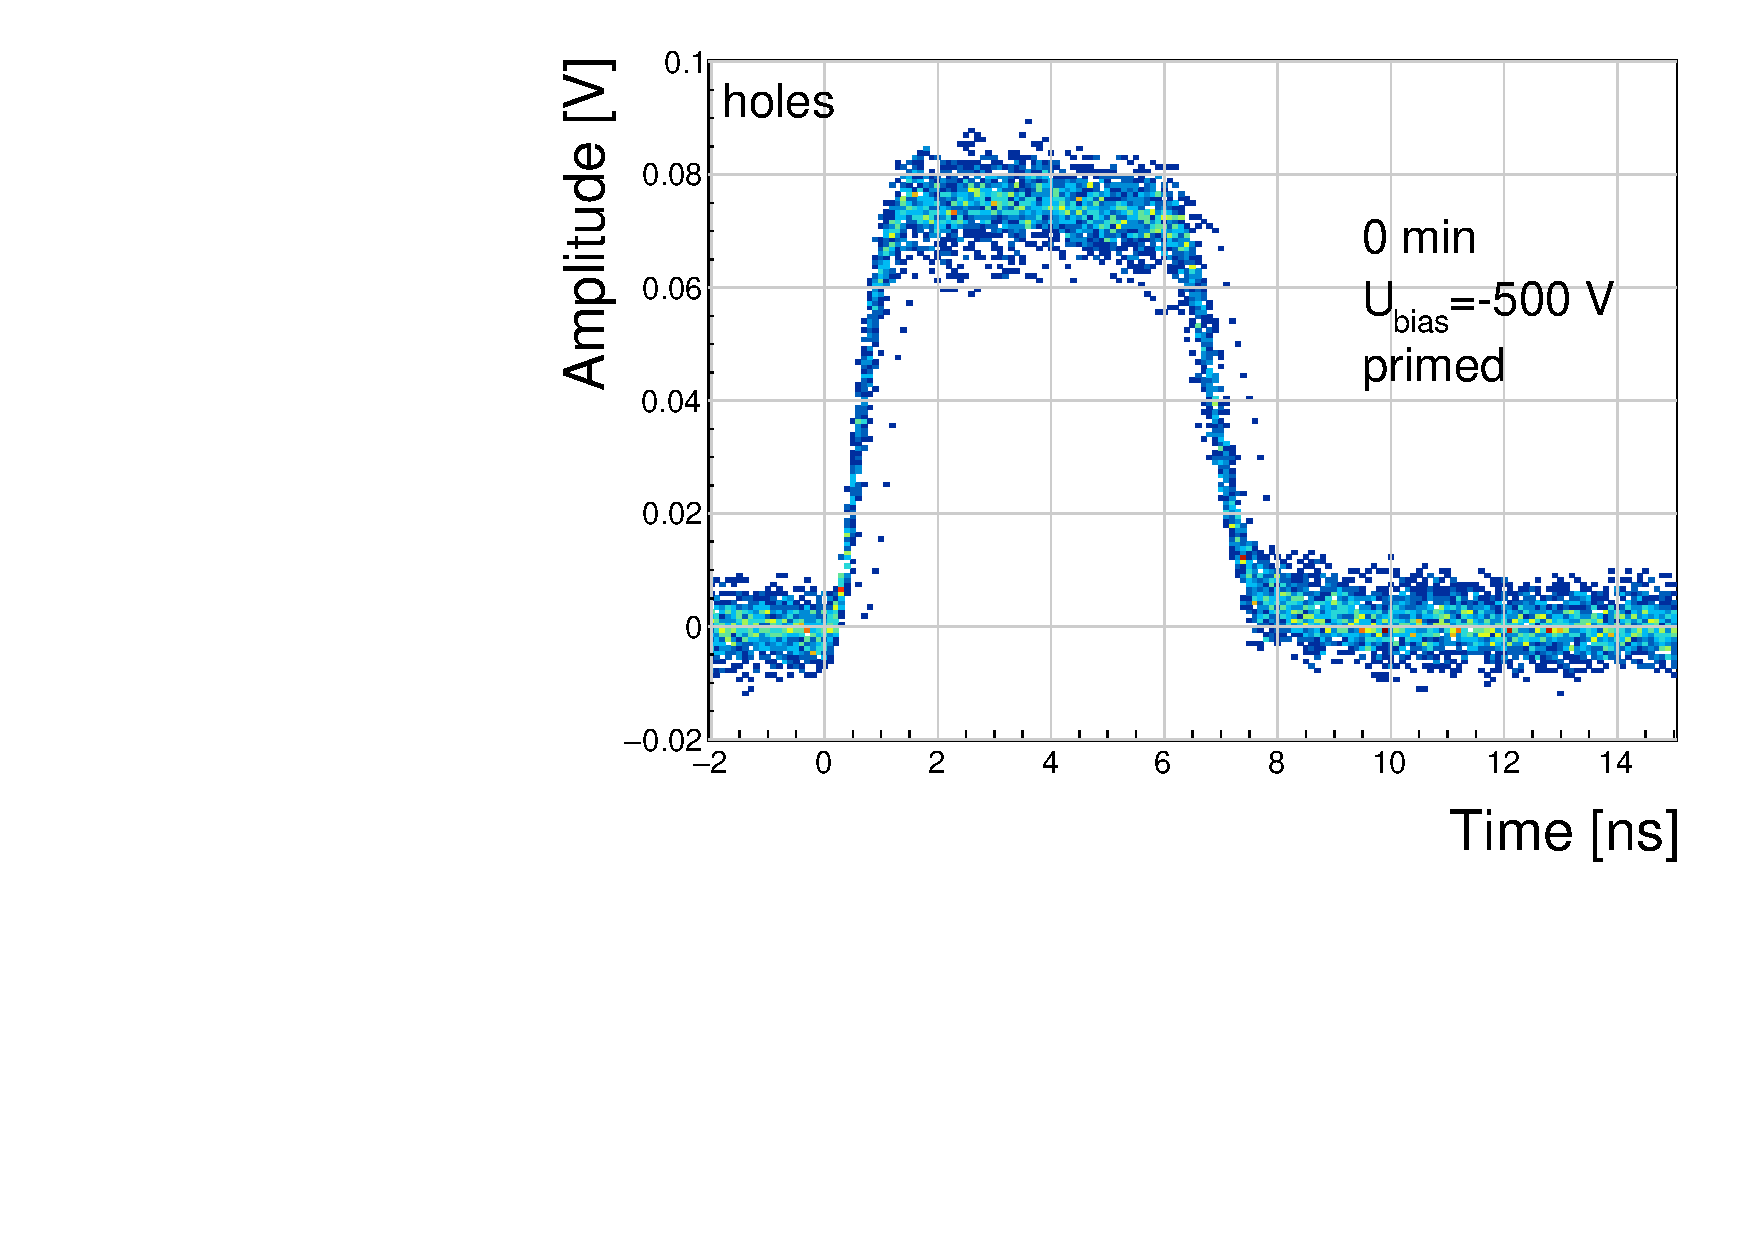
\includegraphics[width=0.30\textwidth]{scripts/plots/plotLifetime/holes0} \label{fig:holes0lt}} &
\subfloat[Holes at 15 min]{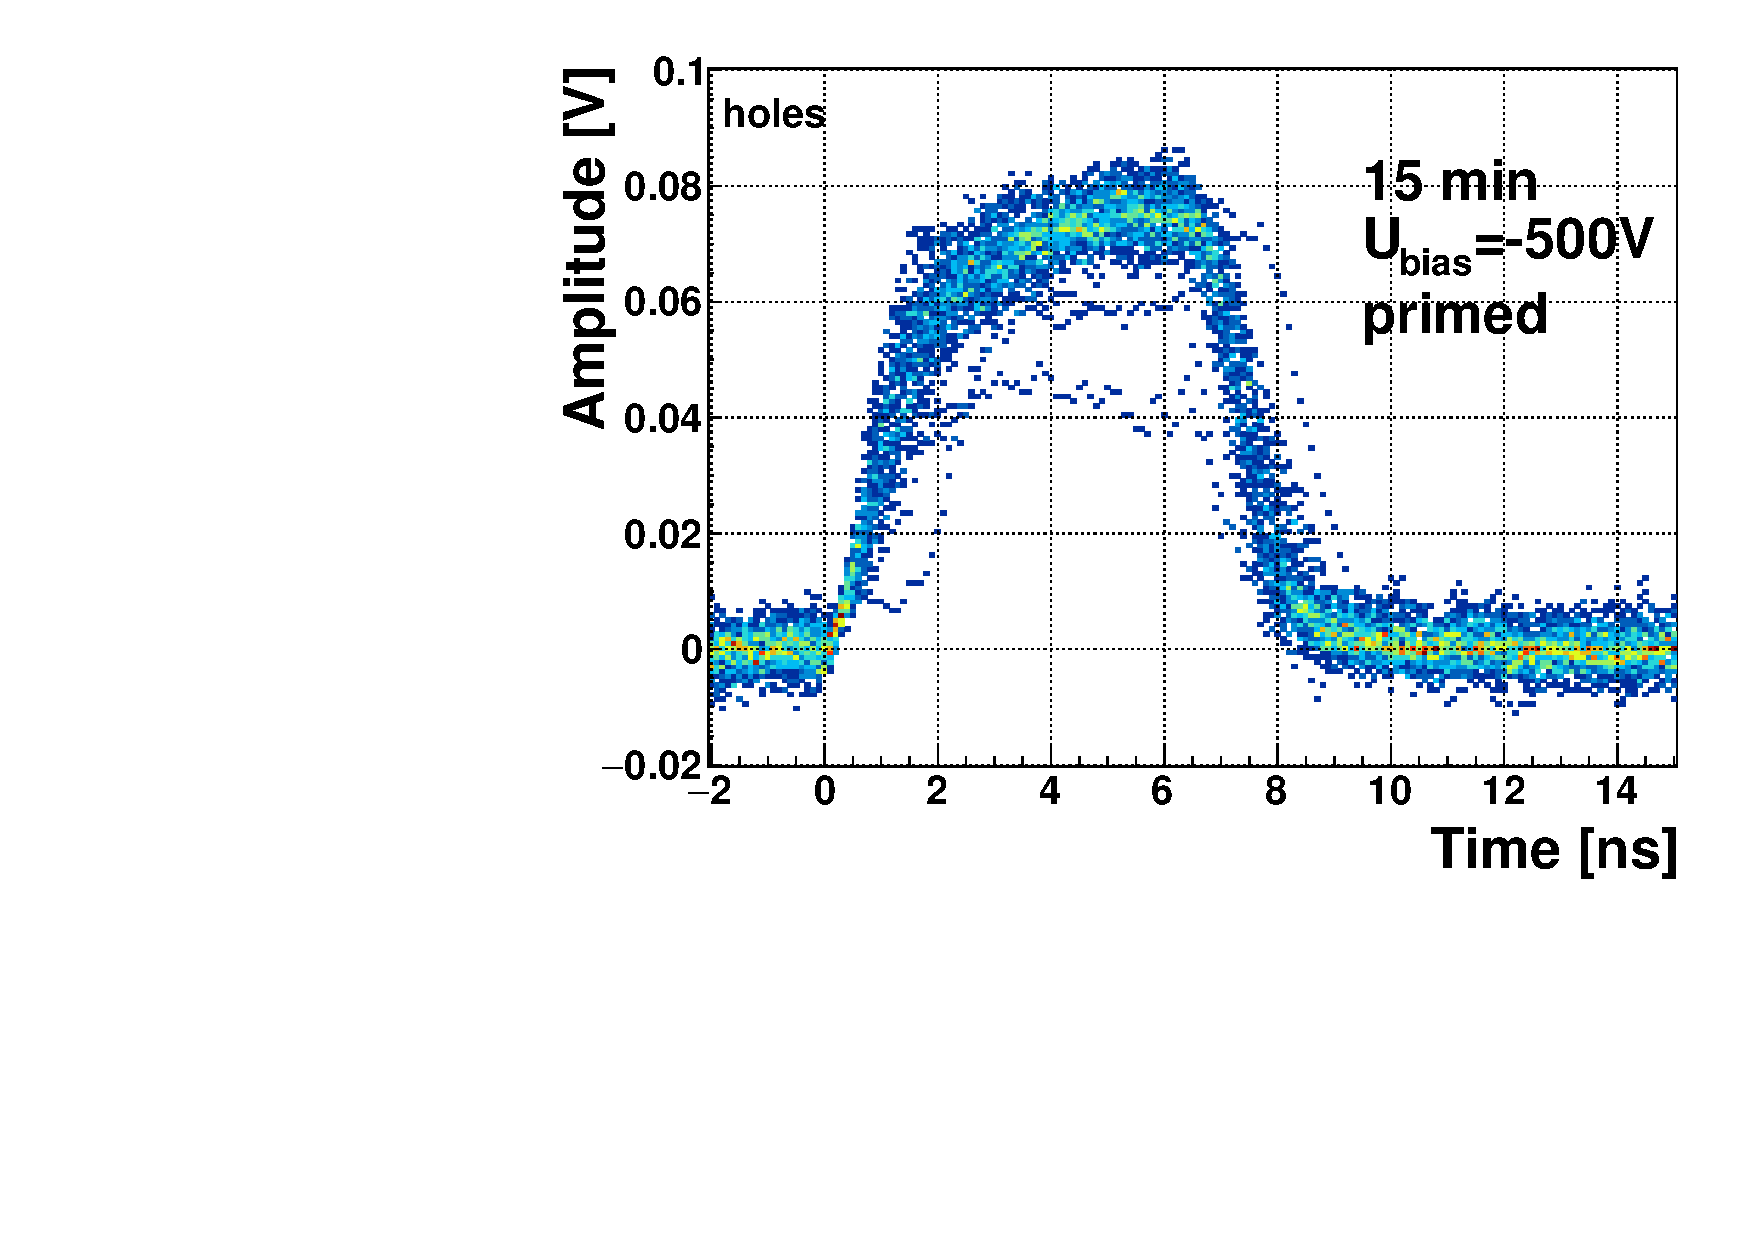
\includegraphics[width=0.30\textwidth]{scripts/plots/plotLifetime/holes15}  \label{fig:holes15lt}} &
\subfloat[Holes at 30 min]{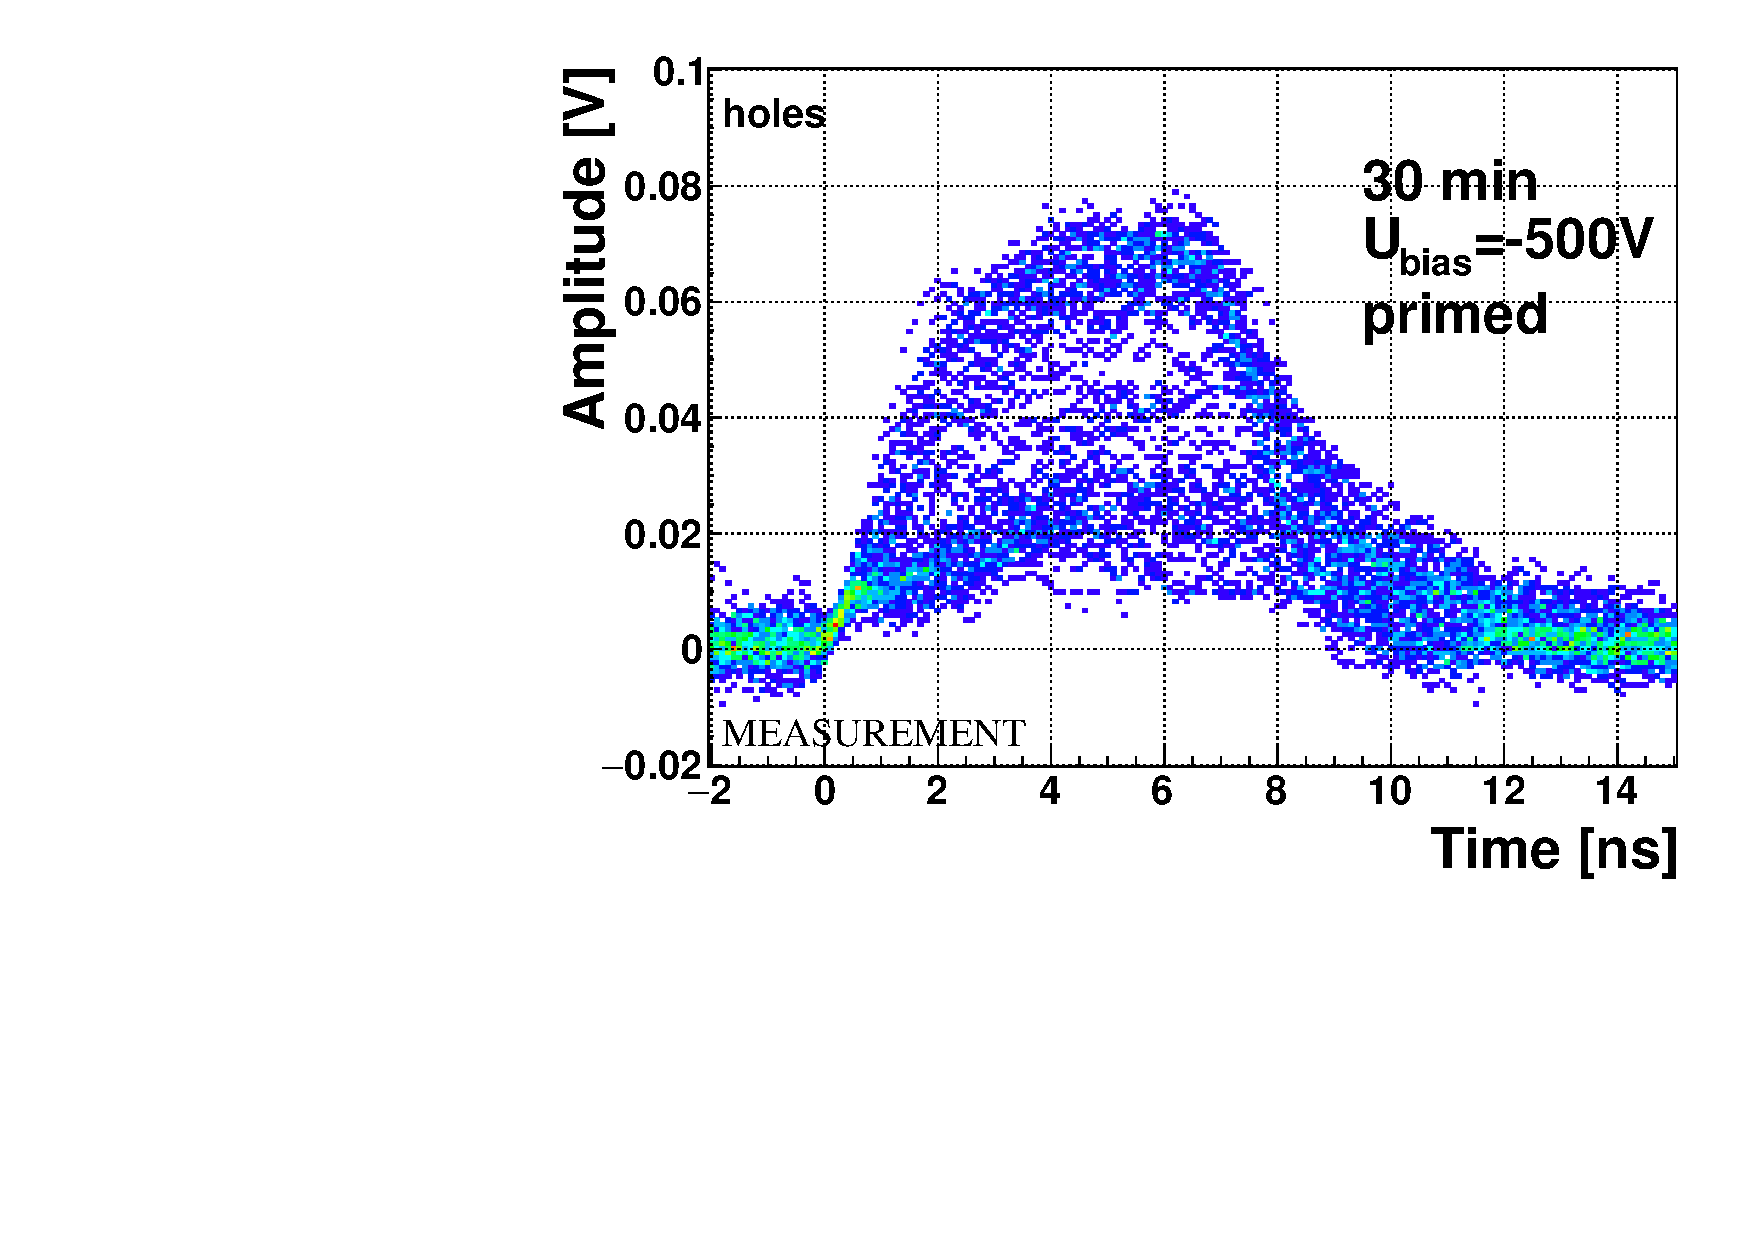
\includegraphics[width=0.30\textwidth]{scripts/plots/plotLifetime/holes30}  \label{fig:holes30lt}} \\
\subfloat[Electrons at 0 min]{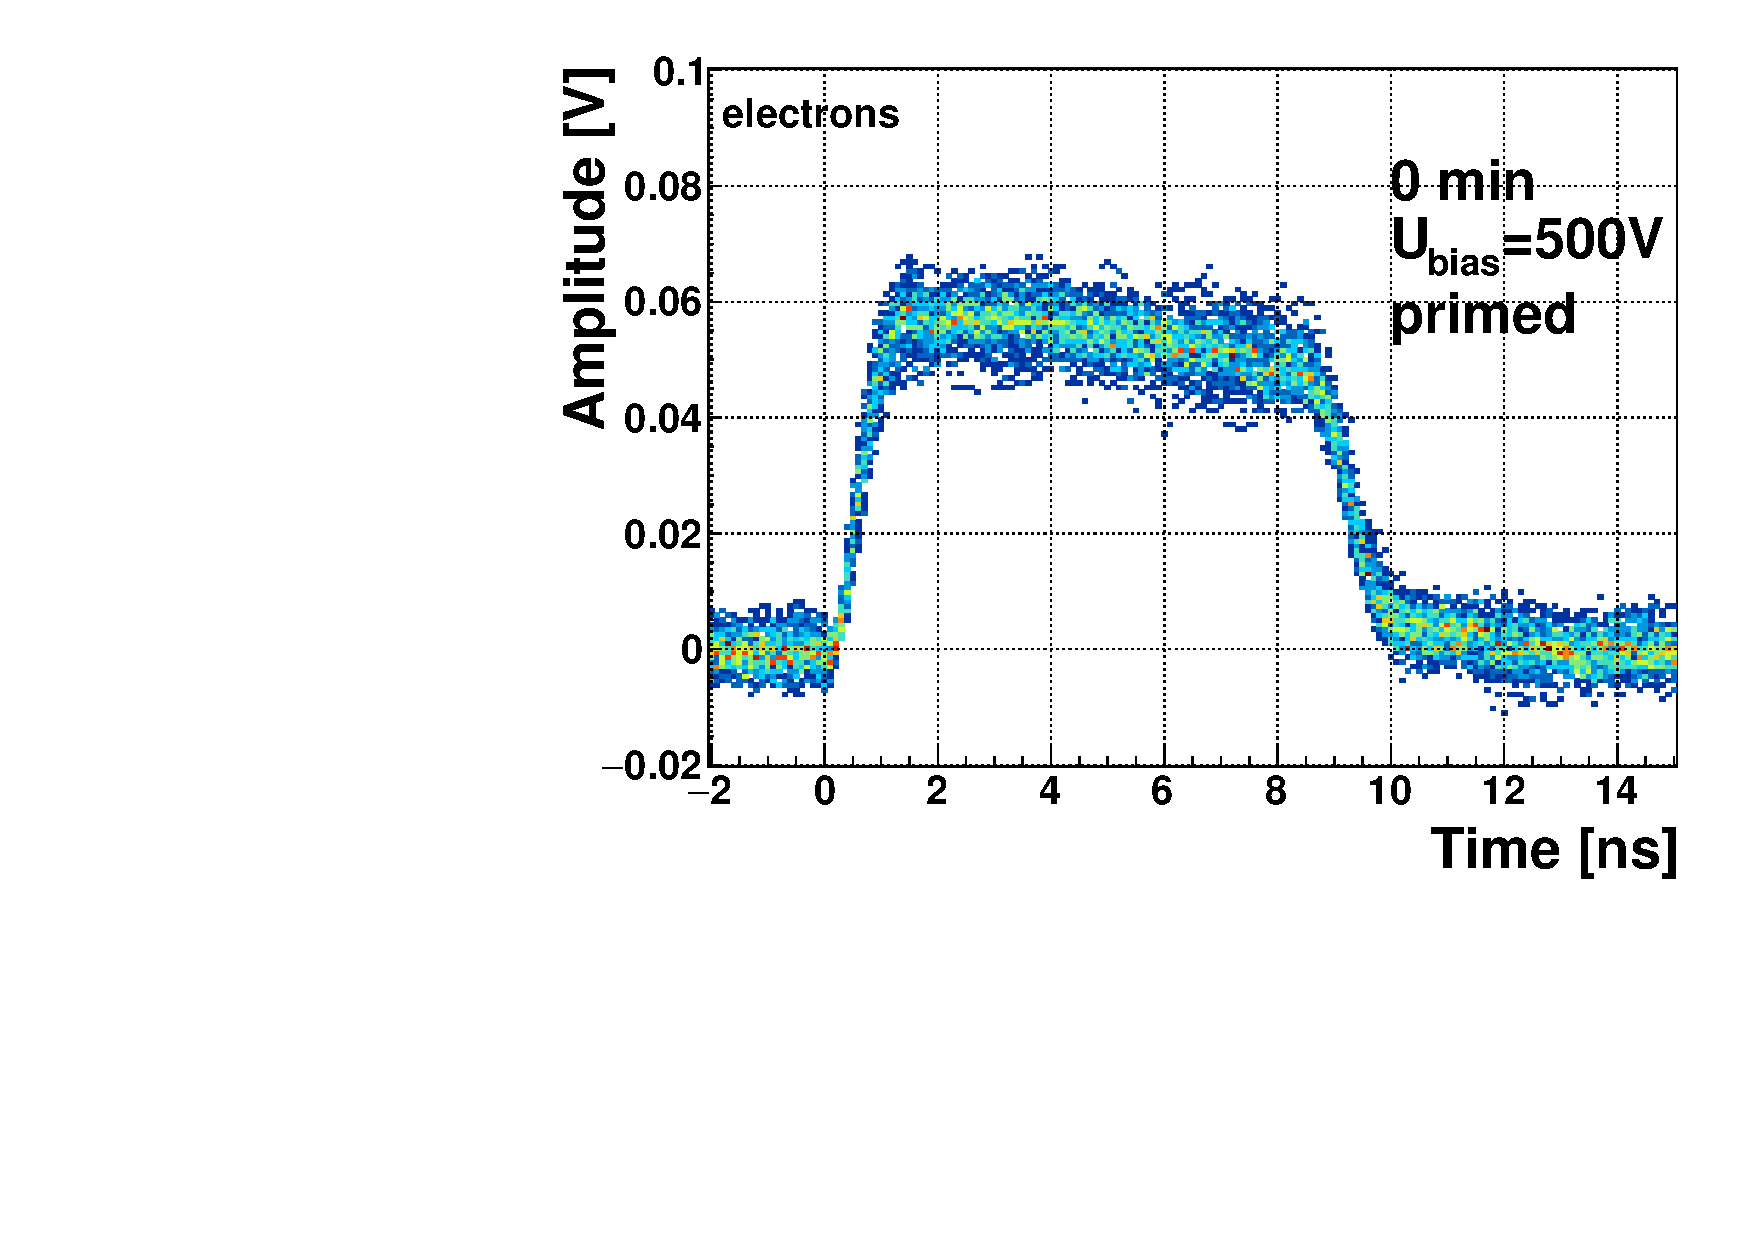
\includegraphics[width=0.30\textwidth]{scripts/plots/plotLifetime/elecs0} \label{fig:elecs0lt}} &
\subfloat[Electrons at 15 min]{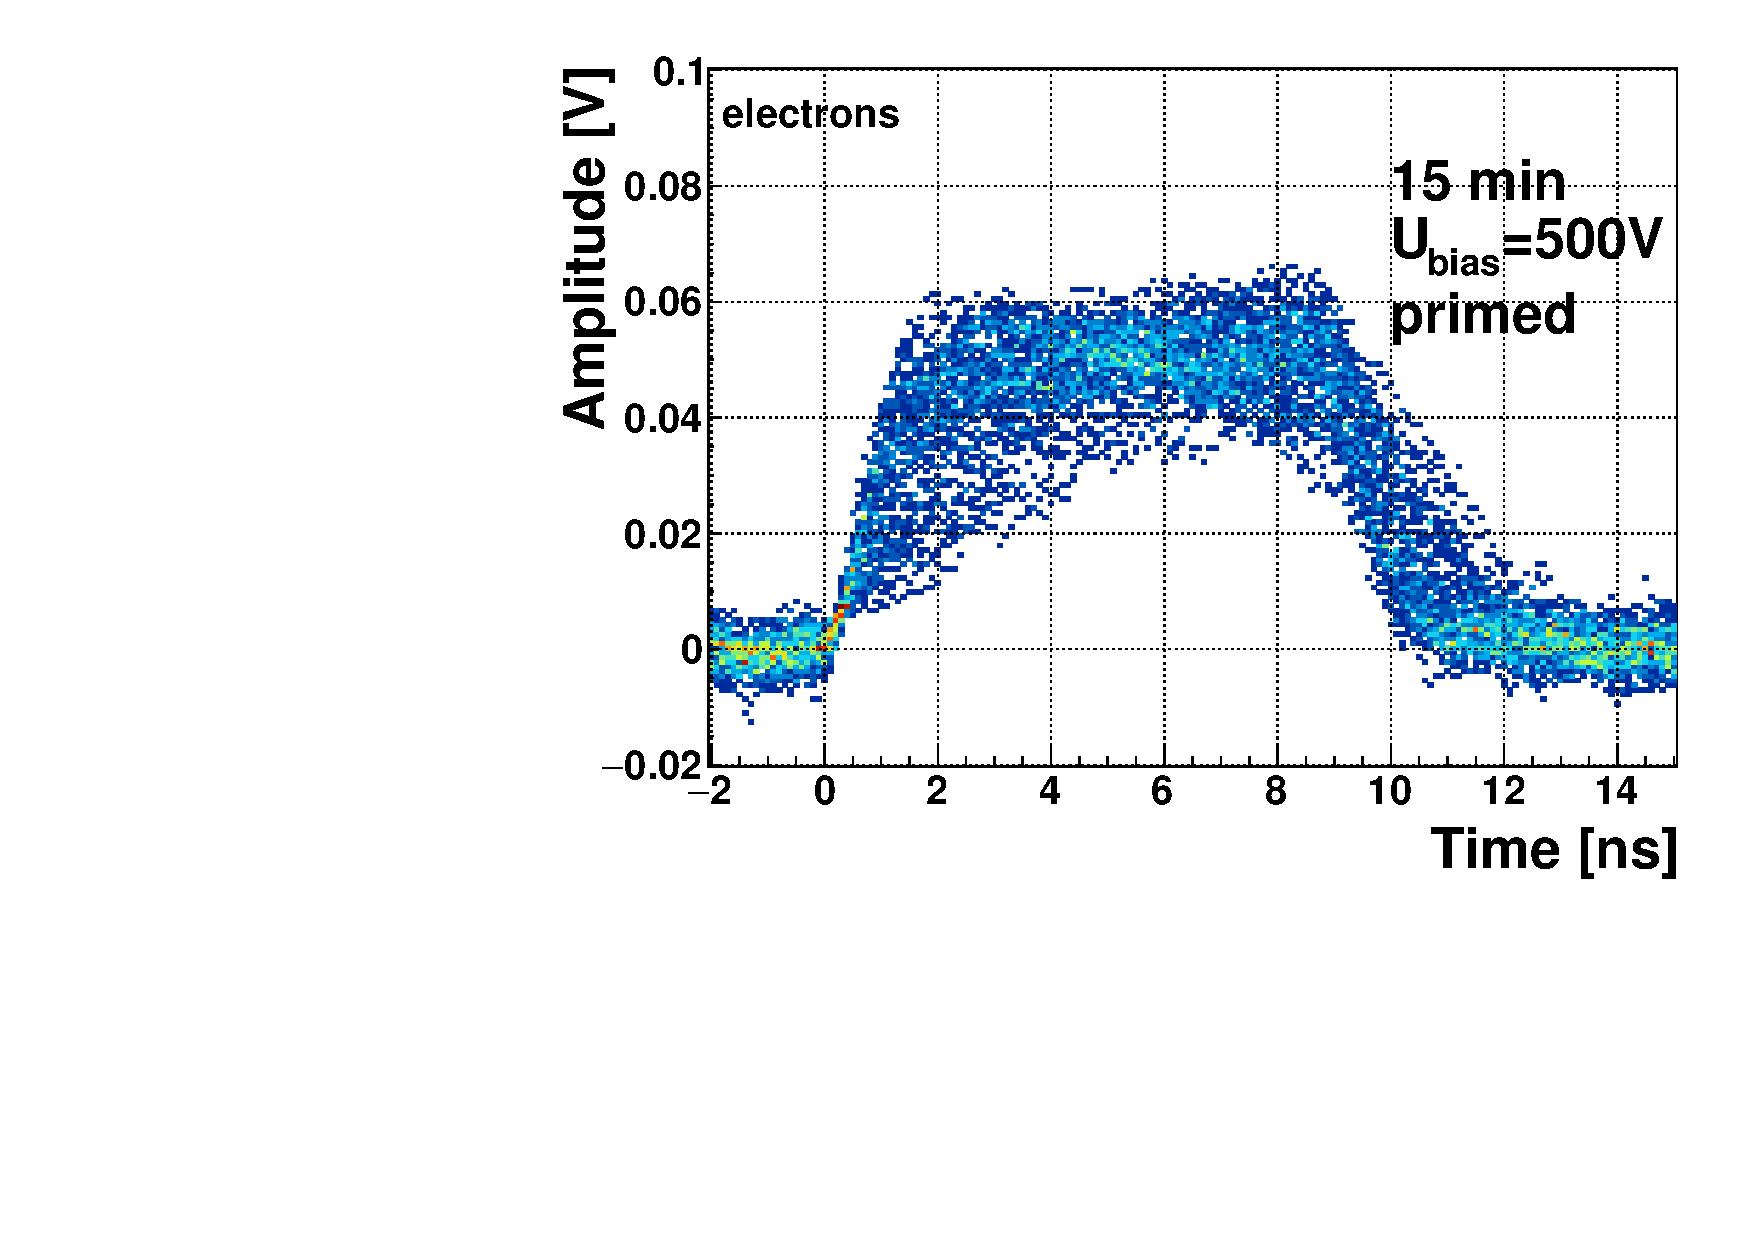
\includegraphics[width=0.30\textwidth]{scripts/plots/plotLifetime/elecs15}  \label{fig:elecs15lt}} &
\subfloat[Electrons at 30 min]{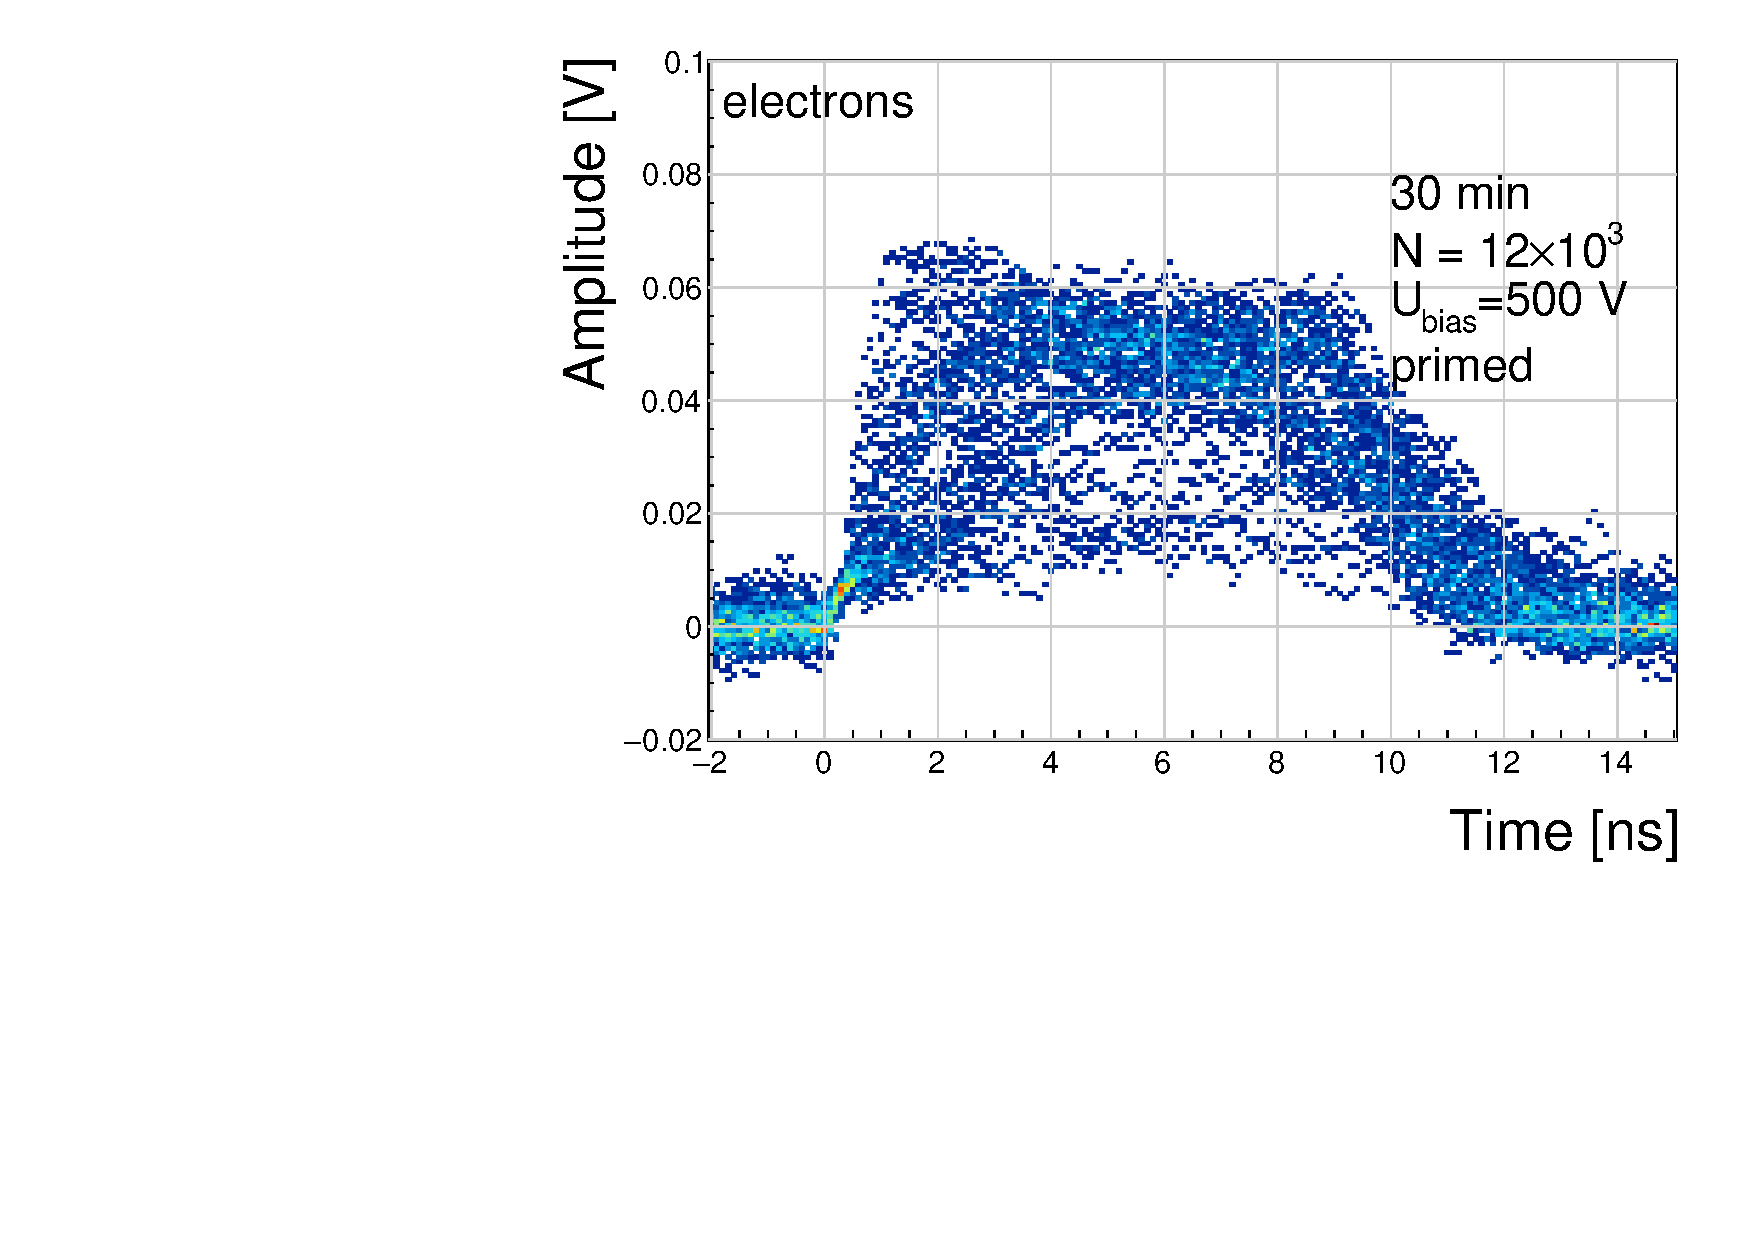
\includegraphics[width=0.30\textwidth]{scripts/plots/plotLifetime/elecs30}  \label{fig:elecs30lt}}
\end{tabular}
\caption{The signal of the irradiated and primed S79 deteriorates with time for both polarities. Every plot contains 60 superimposed pulses.}
\label{fig:lifetimeelecsholes}
\end{figure}

The second test with the C2 current amplifier has been carried out as follows: At the beginning of the test when the diamond is still operating stably, 60 pulses are recorded. An average pulse is calculated. This is a reference pulse for the subsequent measurement points.
% and plotted overlapped into a 2D histogram. An average pulse is extracted from this 2D distribution. 
Then an RMS of the single pulses with respect to the reference pulse is calculated and the values are summed together ($\sigma_\mathrm{ref}$). 

All the subsequent data points also consist of a set of 60 pulses. At every data point the summation of the RMS values of the individual pulses with respect to the initial averaged pulse is calculated ($\sigma$). The ratio between the initial $\sigma_{\mathrm{ref}}$ and discrete values $\sigma$ gives a measure of change of the pulse shape with respect to the reference pulse at the start of the measurement.
%, the shape correlation $Corr_{\mathrm{shape}}$ is calculated:
%\begin{equation}
%\label{eq:correlation}
%Corr_{\mathrm{shape}} (t) = \frac{\sigma_{\mathrm{ref}}}{\sigma} = \frac { \sum_\mathrm{x} \sum_\mathrm{y} w_{\mathrm{ref}}\cdot ( y_{\mathrm{avg}} - y_{\mathrm{ref}})^2 } { \sum_\mathrm{x} \sum_\mathrm{y} w\cdot ( y_{\mathrm{avg}} - y)^2 },
%\end{equation} 
%where $y_{\mathrm{avg}}$ is the amplitude of the current averaged pulse at time $x$, $y_{\mathrm{ref}}$ is the amplitude of the initial averaged pulse at time $x$, $y$ is the amplitude of the superimposed pulses in the 2D histogram and $w$ and $w_{\mathrm{ref}}$ are weights for the superimposed pulses for the current data point and the initial data point.
Figure~\ref{fig:longtermc2corr} shows the ratio $\frac{\sigma_\mathrm{ref} }{\sigma(\alpha~dose)}$. From the data obtained it can be concluded that initial pulse shape quickly starts deteriorating. In fact, the deterioration of the shape correlation follows an exponential decay function, which can be fitted to the data. The resulting decay constants for electrons and holes are $\tau_{\mathrm{corr_e}}=(631\pm20)$~s$^{-1}$ and $\tau_{\mathrm{corr_h}}=(471\pm21)$~s$^{-1}$. The electrons seem to retain the initial shape for longer. The deteriorated shapes also seem to be for a factor of 2 better than those of the holes. 

\begin{figure}[!t]
\begin{center}
\includegraphics[width=0.8\textwidth]{scripts/plots/plotLifetime/corrlifetime}
\caption{Deterioration of the pulse correlation with time }
\label{fig:longtermc2corr}
\end{center}
\end{figure}



Finally, an effort has made to find a way for the pulse shapes to return to their initial state. Five methods were tested: 
\begin{enumerate}[itemsep=0.1\baselineskip]
\item Removing the source and leaving the bias voltage switched on, 
\item Removing the source and switching the bias voltage off, 
\item Priming with $\upgamma$ at a rate of 400~s$^{-1}$cm$^{-1}$ without applied bias voltage, 
\item Priming with $\upbeta$ at a rate of 1000~s$^{-1}$cm$^{-1}$ with applied bias voltage and 
\item Priming with $\upbeta$ at a rate of 1000~s$^{-1}$cm$^{-1}$ without applied bias voltage. 
\end{enumerate}
The diamond sample S79 was first primed using a $^{90}$Sr source for about one hour. Then the bias voltage was switched on and an $^{241}$Am source was put on top. The pulses produced by the impinging $\upalpha$ particles had a proper rectangular pulse at the beginning, but then started changing in an erratic way, as described in the text above. After approximately 30~minutes, one of the methods was tested. When a ``healing'' procedure was started, a set of 60~pulses was taken at irregular points of time to observe the change in the pulse shape and to assess the quality of the ``healing'' procedure. Then the bias voltage was switched off and the sample was primed again to reset its state before starting with the next run. 

It turns out that the methods (3) and (5) improve the shape, method (2) helps slowly, (1) does not show any change with time and (4) at first improves, but then significantly degrades the shape. The effect observed in method (4) has already been described in~\cite{Kramberger}. The ``healing'' process therefore depends on the rate of radiation, the bias voltage and the time of exposure. The ionising radiation creates free charges, which quickly recombine close to the place of generation. It is likely that they also release the charges trapped during the measurement, reducing the overall effect of the space charge. The traps get filled with both flavours of carriers, thus they are neutralised. The pulse shape gradually returns to its initial state.


\begin{footnotesize}
\begin{center}
\begin{tabular}{   c  c  c  c c }
\hline
Procedure & Source & Bias voltage & Effectiveness \\
\hline
1 & / & ON & no \\
2 & / & / & slow \\
3 & $^{60}$Co & / & YES \\
4 & $^{90}$Sr & ON & no \\
5 & $^{90}$Sr & / & YES \\
\hline
\end{tabular}
\captionof{table}{Effectiveness of healing procedures}
\label{tab:healing}
\end{center}
\end{footnotesize}

\begin{figure}[!t]
\begin{center}
\includegraphics[width=0.7\textwidth]{scripts/plots/plotLifetime/formCorrelation}
\caption{Five procedures of the ``healing'' process for an irradiated diamond that was exposed to $\upalpha$ radiation at bias voltage switched on for at least 30~minutes.}
\label{fig:formCorr}
\end{center}
\end{figure}

%TO-DO conclusions: limitations

In summary, the shape of the pulses caused by $\upalpha$ radiation changes with time for irradiated samples. The shape of the pulses gets distorted and becomes erratic. Charge collection decreases and its spread increases. This happens even faster for non-primed diamonds. To ``heal'' the diamond -- to bring the pulse shapes back to their initial shape -- the sample must be primed using a $\upbeta$ or a $\upgamma$ source for several minutes at the bias voltage set to 0~V. Switching to the inverse polarity for a few seconds helps a bit, but in a long run distorts the signal, which cannot get back to its initial shape.

















% ---------------------------------------------------------------------------------------------------------------
%\clearpage
\section{Temperature limitations}
\label{sec:templimit}
% ---------------------------------------------------------------------------------------------------------------
A test has been carried out to evaluate the effect of temperature changes on the output signal of the diamond sensors. A cryostat filled with liquid helium is used to cool down the sensor during the measurement process. The current signal response to $\alpha$-particles is measured at 18 temperature points between 4~K and 295~K. At every temperature point, a set of 300 pulses is read out at various bias voltages. Resulting data show that the charge collection is stable down to 150~K, where it starts decreasing and stabilises again at about one third of the initial value at 75~K. This behaviour was first measured and discussed by H. Jansen~\cite{JansenThesis}.

%\subsubsection{Acoustic phonon scattering}
The band gap energy in diamond is equal to $E_\mathrm{g}=5.5$~eV while the average energy to produce an electron-hole pair is $E_{\mathrm{e-h}}=13.25$~eV. This means there is excessive energy deposited in the diamond bulk. The incident $\upalpha$-particle stops within $\sim$10~$\upmu$m of the bulk, transferring all its energy to the lattice. A part of this energy, approximately 40~\%~\cite{}, directly ionises the carbon atoms, creating free electron-hole pairs. The positively charged hole and the negatively charged electron in the hole attract each other via the Coulomb force and may undergo a bonding process during which a phonon is emitted. 

The remaining energy, however, is converted into lattice vibrations (phonons~\cite{Phonons}). This means that the lattice within the ionisation volume (approximately $\sim$10~$\upmu$m$\times\sim$2~nm in size) is briefly heated up. The hot plasma then cools down to the temperature of the surrounding material by heat dissipation, (i.e. phonon transport).
%\subsubsection{Exciton formation and recombination}
%That phonon is referred to as \emph{exciton}~\cite{Exciton}. 
The free electron binds the free hole into a bound state (not recombination) -- the exciton~\cite{}. The exciton binding energy is 80~meV. At higher temperatures, the lattice provides enough energy to excite the electron from the exciton state back to the conduction band. At lower temperatures, however, the exciton lifetime increases, which means that it will take a longer time for the electrons to get re-excited to the conduction band. The re-excitation lifetime at room temperature is $\sim$30~ps, increasing to $\sim$150~$\upmu$s at 50~K~\cite{}. This means that some of the bound electrons will not even start drifting within the period of $\sim$10~ns, which is the expected carrier drift time. When they are finally freed, the current they induce is already hidden in the electronics noise. The effective area of the observed current pulse is therefore smaller than that of a pulse induced by all the carriers drifting at the same time. This in effect reduces the measured collected charge. The longer the time constant, the lower the measured collected charge, as shown in figure~\ref{fig:chgtemp} below.


%The irradiated samples were put in the cryostat, which was cooled down to 4.2~K using liquid helium. TCT data were then taken at a range of bias voltages at temperature points ranging between 4.2~K and room temperature (RT). The results showed that irradiation causes forming of charge traps in the bulk.l;'
%
%TO-DO: get the Tau and plot it against T. 
%TO-DO: plot the drift time against square voltage.


\subsection{Temperature-variant $\upalpha$-TCT before irradiation}
% Show a set of pulses
Three sCVD diamond samples have been tested at a range of temperatures using the $\upalpha$-TCT technique. At each temperature point, the bias voltage is set to several positive and negative values. A set of 300 pulses is recorded at every data point and averaged offline. The resulting averaged pulses of sample S37 at the 260~K temperature point and a bias voltage of $\pm$400~V, $\pm$500~V and $\pm$700~V are shown in figure~\ref{fig:voltpulse}. The pulses induced by holes as charge carriers are shorter than those induced by electrons, which means that holes travel faster in diamond. The area of the pulse, however, is the same for both polarities, which corresponds to the fact that the same amount of charges is drifting in both cases.

\begin{figure}[!t]
\begin{tabular}{rr}
\subfloat{\includegraphics[width=0.47\textwidth]{scripts/plots/pulsesVolt/varVolt_S52_elecs_260k} \label{fig:S52cTplus}} &
\subfloat{\includegraphics[width=0.47\textwidth]{scripts/plots/pulsesVolt/varVolt_S52_holes_260k}  \label{fig:S52ctTminus}}
\end{tabular}
\caption{Varied bias voltage at a fixed temperature}
\label{fig:voltpulse}
\end{figure}

Figure~\ref{fig:temppulses} shows pulses at a bias voltage set to $\pm500$~V across the range of temperatures between 4~K and 295~K -- room temperature (RT). Several conclusions can be drawn by observing their shape. First, the pulse shapes change with decreasing temperature. The pulse time gets shorter, hinting at the faster carrier drift velocity $v_{\mathrm{drift}}$. Second, between 150~K and 75~K there is a significant change in shape - the time constant of the rising edge increases significantly and the pulse area decreases. From 75~K down to 4~K there is no significant observable change. Last, the top of the pulse at the S52 is not flat, which means that a portion of the drifting charge is lost along its way.  This is due to charge trapping, likely by means of crystal defects or impurities.

%This could be due to impurities in the diamond bulk, which act as charge traps, or due to the space charge built up in the bulk. A linear pulse top hints on the latter. All in all, the pulse shape changes significantly with temperature, which is predicted by Jansen's model.

\begin{figure}%[!t]
\begin{tabular}{rr}
\subfloat{\includegraphics[width=0.47\textwidth]{scripts/plots/pulses/S37_elecs} \label{fig:S37plus}} &
\subfloat{\includegraphics[width=0.47\textwidth]{scripts/plots/pulses/S37_holes}  \label{fig:S37minus}} \\
\subfloat{\includegraphics[width=0.47\textwidth]{scripts/plots/pulses/S79_elecs} \label{fig:S79plus}} &
\subfloat{\includegraphics[width=0.47\textwidth]{scripts/plots/pulses/S79_holes}  \label{fig:S79minus}} \\
\subfloat{\includegraphics[width=0.47\textwidth]{scripts/plots/pulses/S52_elecs} \label{fig:S52plus}} &
\subfloat{\includegraphics[width=0.47\textwidth]{scripts/plots/pulses/S52_holes}  \label{fig:S52minus}}
\end{tabular}
\caption{Several data points between 4~K and 295~K at a bias voltage of $\pm$500~V}
\label{fig:temppulses}
\end{figure}


% TO-DO Show drift velocity wrt volt
% TO-DO Show drift velocity wrt temp
% TO-DO Show integrated charge
% TO-DO Show Vdrift wrt 1/Voltage
%$(1\pm0.2)\times10^{14}~\pi~cm^{-2}$ and $(3.63\pm0.76)\times10^{14}~\pi~cm^{-2}$. 

\subsection{Temperature-variant $\upalpha$-TCT after irradiation}
The irradiated S79 and S52 have been re-tested in the cryostat after irradiation. The aim was to see how their pulse shapes change with decreasing temperature, in particular the decaying top of the pulses (see figure~\ref{fig:voltpulseAfter}). The decay time gives information on trapping of charge carriers while travelling through the diamond bulk. A variation of the decay time constant as a function of temperature might help to reveal the type and depth of the charge traps. To observe these effects or lack thereof, a number of requirements has to be met. First, the diamond samples are intentionally not primed prior to the experiment because priming would improve the pulse shapes and possibly change the decay time constant of the signal. Second, keeping in mind that the pulse shape of irradiated diamonds changes with time, the duration of the measurement of an individual data point has to be short -- of the order of 30~seconds. Last, the sequence of the bias voltage settings is important, the reason for which is explained below.

Unfortunately it is not possible to avoid temporal pulse changes. For instance, one measurement point takes approximately one minute. After the measurement, the bias voltage polarity is swapped for a few seconds to bring the diamond back into its initial state. But a few seconds with respect to a minute is not enough. Therefore, when the bias voltage is set to the next value, there is still some residual effect of the previous measurement. Similar to the effects of polarisation, this effect is also decreasing the pulse height. This can be observed in figure~\ref{fig:voltpulseAfter}, which shows the resulting pulses of S52 for bias voltages of $\pm$200~V, $\pm$300~V, $\pm$400~V and $\pm$500~V at 230~K and 260~K. In this case the measurements sequence is: 230K (200~V, 300~V, 400~V, 500~V, -500~V, -400~V, -300~V), 260~K (-200~V, -300~V, -400~V, -500~V, 500~V, 400~V, 300~V). The changes in pulse shapes for holes at 230~K and 260~K cannot be attributed to the temperature change. Instead, the explanation could lie in diamond ``polarisation''. This means that, when exposed to an electric field with $\upalpha$ measurements ongoing, the diamond builds up an internal electric field of inverse polarity, which effectively reduces the overall electric field. This internal field does not dissipate when the external bias voltage is switched off. It can be said that the diamond becomes ``polarised''. When switching the polarity of the external bias voltage, the internal and external electric field point in the same direction at the beginning, increasing the overall electric field and with it the pulse height. In figure~\ref{fig:voltpulseAfter}, this happens when switching from 500~V (figure~\ref{fig:S52cTplusAfter230}) to -500~V (figure~\ref{fig:S52cTminusAfter230}) at 230~K. The built up polarisation contributes to the pulse having a sharp rising edge and a high amplitude. This effect decays during the next two voltage points. There would be a handful of ways to avoid this polarisation effect in the data: 

\begin{enumerate}[itemsep=0.1\baselineskip]
\item After every data point invert the bias voltage and leave it to return to a neutral state for the same amount of time, 
\item Make a hysteresis of data points, going from minimum negative to maximum positive bias several times, 
\item Reduce the measurement time at every bias voltage setting.
\end{enumerate}
Unfortunately, options (1) and (2) are very time consuming and would increase the overall experiment time to over one day. The third option would worsen the resulting averaged pulses. In the end an alternative option was chosen: alternating the starting bias voltage and the sequence at every temperature point. With this option, a meaningful systematic error in analysing the pulse shapes can be attained.

\begin{figure}[!t]
\begin{tabular}{rr}
\subfloat{\includegraphics[width=0.47\textwidth]{scripts/plots/pulsesVolt/varVolt_S52_3-63e14_elecs_230k} \label{fig:S52cTplusAfter230}} &
\subfloat{\includegraphics[width=0.47\textwidth]{scripts/plots/pulsesVolt/varVolt_S52_3-63e14_holes_230k}  \label{fig:S52ctTminusAfter230}} \\
\subfloat{\includegraphics[width=0.47\textwidth]{scripts/plots/pulsesVolt/varVolt_S52_3-63e14_elecs_260k} \label{fig:S52cTplusAfter260}} &
\subfloat{\includegraphics[width=0.47\textwidth]{scripts/plots/pulsesVolt/varVolt_S52_3-63e14_holes_260k}  \label{fig:S52ctTminusAfter260}}
\end{tabular}
\caption{Varied bias voltage at a fixed temperature for an irradiated sample}
\label{fig:voltpulseAfter}
\end{figure}


Figure~\ref{fig:temppulsesAfter} shows the irradiated S52 and S79 as well as the non-irradiated S37 for comparison, all at a bias voltage of $\pm$500~V and at several temperature points between 4~K and RT. It is evident that the radiation damage affected the shape of the pulses across all temperatures. 


\begin{figure}[!t]
\begin{tabular}{rr}
\subfloat{\includegraphics[width=0.47\textwidth]{scripts/plots/pulses/S37_elecs} \label{fig:S37plusAfter}} &
\subfloat{\includegraphics[width=0.47\textwidth]{scripts/plots/pulses/S37_holes}  \label{fig:S37minusAfter}} \\
\subfloat{\includegraphics[width=0.47\textwidth]{scripts/plots/pulses/S79_1e14_elecs} \label{fig:S79plusAfter}} &
\subfloat{\includegraphics[width=0.47\textwidth]{scripts/plots/pulses/S79_1e14_holes}  \label{fig:S79minusAfter}} \\
\subfloat{\includegraphics[width=0.47\textwidth]{scripts/plots/pulses/S52_3-63e14_elecs} \label{fig:S52plusAfter}} &
\subfloat{\includegraphics[width=0.47\textwidth]{scripts/plots/pulses/S52_3-63e14_holes}  \label{fig:S52minusAfter}}
\end{tabular}
\caption{After irradiation: several data points between 4~K and 295~K at a bias voltage of $\pm$500~V}
\label{fig:temppulsesAfter}
\end{figure}


\subsubsection{Collected charge as a function of temperature}
The area below the current pulse is proportional to the charge collected by the diamond detector. The collected charge is observed as a function of temperature. First, the amplitude values of the averaged pulses at a bias voltage of $\pm$500~V and across the temperature range between 4~K and 295~K have to be integrated. Then a calibration factor is used to derive the charge for all data points. This factor is obtained using a Cx charge-sensitive amplifier. The resulting values for electrons and holes are plotted in figures~\ref{fig:chgtempelecs} and~\ref{fig:chgtempholes}, respectively. Thesis~\cite{} gives a model that explains the drop in charge below 150~K. The new contribution are the data points for the irradiated samples. The values for them are lower than the those of non-irradiated samples, which is expected.

The values for all samples are fairly stable in the range between 4~K and 75~K and between 150~K and 295~K. However, in the values for the irradiated S52 some excursions can be observed. This is due to the sequence of the measurement steps, which introduced a hysteresis effect and is explained in the preceding text.

The collected charge drops significantly from 150~K down to 75~K. In the non-irradiated samples the values in the lower temperature range are approximately 0.30 of the values at the high range. For the irradiated ones this difference is lower -- a factor of 0.35 for S79 and 0.5 for S52. An interesting detail is that the ratio between the values for non-irradiated samples and their irradiated counterparts  at the lower range is different than at the higher range. Looking at the values for the electron collection in figure~\ref{fig:chgtempelecs}: for S52 the lower ratio is equal to 1.28 and the higher equal to 1.7. For S79 these ratios are 1.00 and 1.09, which means that the difference in charge collection between 4~K and 75~K before and after irradiation is negligible.

\begin{figure}[!t]
\begin{tabular}{cccc}
\subfloat{\includegraphics[width=0.80\textwidth]{scripts/plots/charge500V} \label{fig:chgtempelecs}} \\
\subfloat{\includegraphics[width=0.80\textwidth]{scripts/plots/charge-500V}  \label{fig:chgtempholes}}
\end{tabular}
\caption{Collected charge as a function of temperature}
\label{fig:chgtemp}
\end{figure}



\subsubsection{Charge trapping}
A decaying exponential function has been fitted to the decaying top of the averaged pulses at bias voltages of $\pm$400~V and $\pm$500~V across all temperatures excluding the transitional range between 75~K and 150~K. The resulting decay time constants $\tau$ for an individual temperature point are not equal, which stems from the fact that the pulses change with time due to ``polarisation''. This counts as a systematic error. Therefore the fitted $\tau$ for $\pm400$~V and $\pm500$~V are averaged into one value representing the measurement at that temperature point. Figure~\ref{fig:lifetimevstemp} shows the fitted $\tau$ for the five samples between 4~K and 295~K. In principle, the time constants should be infinite for a perfect and non-irradiated sample. Here a slightly tilted top of the pulse due to space charge is already successfully fitted with an exponential function, resulting in a $\tau$ of the order of (200$\pm$20)~ns$^{-1}$. Consequently the fitting method is not adequate for non-irradiated samples. For the irradiated samples, the fit becomes increasingly more meaningful. As seen in figure~\ref{fig:lifetimevstemp}, the fitted values of the irradiated samples are fairly stable across all temperatures. There is a slight increase in the decay time constant of the S52 from $(6.0\pm0.5)$~ns$^{-1}$ above 150~K to ($8.5\pm0.9$)~ns$^{-1}$ below 75~K. On the other hand, this step is not observable in the S79 data. With only one sample exhibiting this behaviour, the effect is not significant enough. Judging by the data acquired, the samples would need to be irradiated to doses above $1\times10^{14}~\uppi~$cm$^{-2}$ to quantify this effect in detail. So far this effect will not be regarded as significant for the scope of this thesis. Building on this assumption, the conclusion is that the signal decay time constant for irradiated sCVD diamond is constant across the temperature range between 4~K and 195~K, excluding the transitional range between 75~K and 150~K. 

Taking into account the conclusions above, all the values can be averaged into one decay constant. Figure~\ref{fig:lifetimevsdose} shows these values for all samples as a function of the received $\uppi_\mathrm{300~MeV}$ radiation dose. To estimate the carrier lifetime with respect to the radiation dose received, a similar model is used than that in section~\ref{sec:radlimit}. This model states that the inverse of the carrier lifetime is linearly decreasing with increasing radiation dose:
\begin{equation}
\label{eq:ltfactor}
\frac{1}{\tau} = \frac{1}{\tau_\mathrm{0}}+\kappa_{\mathrm{\tau}}\cdot\Phi
\end{equation} 
\begin{equation}
\label{eq:ltfactor1}
\tau = \frac{\tau_\mathrm{0}}{\kappa_{\mathrm{\tau}} \tau_\mathrm{0} \Phi + 1}
\end{equation} 
where $\tau_\mathrm{0}$ is the lifetime for a non-irradiated sample (real lifetime, therefore of the order of 400~ns$^{-1}$), $\tau$ is the lifetime of an irradiated sample, $\Phi$ is the received radiation dose and $\kappa_{\mathrm{\tau}}$ the lifetime degradation factor. For these data the fitted factor is equal to $\kappa_{\mathrm{\tau}}=(3.6\pm0.8)\times10^{-16}~$s~cm$^2$~$\uppi_{\mathrm{300~MeV}}^{-1}$. Using this factor, the steepness of the decay in the pulse shape with respect to radiation dose can be estimated. This can help when designing a system where current pulse shape is an important factor.
%introduce the kTau factor

\begin{figure}[!t]
%\centering
\begin{tabular}{cccc}
\subfloat[Carrier lifetime as a function of temperature]
{\includegraphics[width=0.8\textwidth]{scripts/plots/taunew/lifetimevstemp} \label{fig:lifetimevstemp}} \\
\subfloat[Carrier lifetime averaged over all temperatures as a function of $\pi$ irradiation dose]{\includegraphics[width=0.8\textwidth]{scripts/plots/taunew/avglifetime}  \label{fig:lifetimevsdose}}
\end{tabular}
\caption{Charge carrier lifetime decreases with irradiation, but is stable across the range of temperatures between 4~K -- 75~K and 150~K -- 295~K.}
\label{fig:carrlifetime}
\end{figure}










% ---------------------------------------------------------------------------------------------------------------
%\clearpage
\section{Conclusion}
\label{sec:radlimit}
% ---------------------------------------------------------------------------------------------------------------
This chapter gives an overview of the capabilities and limitations of diamond as a particle detector. Three effects on diamond were studied -- noise, radiation and temperature, the focus being on the latter two. 

Two sCVD diamond detectors were irradiated with 300~MeV pions. They were tested alongside a non-irradiated sample to observe the changes in the ability to detect $\upalpha$, $\upbeta$ and $\upgamma$ radiation. Their charge collection efficiency was measured in a test beam facility using . The results were compared to the results from the RD42 collaboration and a DPA model~\cite{}. A radiation damage factor $k_{\mathrm{\lambda}}=(3.0\pm1.0)\times10^{-18}~\upmu$m$^{-1}$~cm$^{-2}$ was obtained for $\uppi_{\mathrm{300~MeV}}$ particles. The data point was not in agreement with the data provided by RD42 nor with the model. However, the irradiation process and the low number of tested samples hold a relatively high statistical uncertainty. In addition, there was no diamond surface treatment done in between the measurements, as is the case in the study conducted by RD42. The results obtained in the course of these measurements will also be fed into the existing pool of data in the RD42 collaboration.

The next step was to test the long-term capabilities for $\upalpha$ detection. The shape of the ionisation profile was investigated to determine the behaviour of the charge carriers in the irradiated diamond. An exponential decay was observed in the pulses of irradiated samples, proving that there are charge traps in the bulk that were created during irradiation. Then a long-term stability test was carried out. The results show that the irradiated diamond detectors do not provide a stable and reliable long-term measurement of $\upalpha$ particles. This might be due to a space-charge build-up in the bulk, which changes the electric field, affecting the charge carriers. A procedure to improve the pulse shape using $\upbeta$ and $\upgamma$ radiation was proposed.

Finally, the diamond sensors were cooled down to temperatures between 4~K and 295~K. Their response to $\upalpha$ particles was observed. The results of the non-irradiated and irradiated samples were compared. The effect of reduction for the number of drifting charges due to exciton recombination was observed in both sets of data. The second set had a superimposed effect of charge trapping during the drift, which was represented by an exponential decay in the signal. The decay time constant did not change with temperature. Therefore all temperature points for individual samples were averaged and the decay time constants were plotted against the received radiation dose. A damage factor equal to $\kappa_{\mathrm{\tau}}=(3.6\pm0.8)\times10^{-16}$~s~cm$^2$~$\uppi_{\mathrm{300~MeV}}^{-1}$ for non-primed diamonds was defined.



% ---------------------------- comment out when compiling the full document -------------------
\end{document}
% ---------------------------------------------------------------------------------------------------------------

% ---------------------------------------------------------------------------------------------------------------
\Chapter{Charge monitoring}{The ATLAS Diamond Beam Monitor}
%\chapter{Charge monitoring}
% ---------------------------------------------------------------------------------------------------------------

%-Diamond Beam Monitor
%
%-Spatial segmentation
%
%-FE-I4
%
%-Desc of ATLAS pixel module, functions
%
%-Why do we use diamond in combination with FEI4
%
%-Construction of 24 modules
%
%-Performance results (main part)
%
%-source tests
%
%-desy testbeam (spacial resol, efficiency, TOT)
%
%-Problems, limitations
%
%-Commissioning, installation
%
%-Comparison between diamond and silicon modules.


Particle detectors in high energy physics experiments need to meet very stringent specifications, depending on the functionality and their position in the experiment. In particular, the detectors close to the collision point are subject to high levels of radiation. Then, they need to operate with a high spatial and temporal segmentation to be able to precisely measure trajectories of hundreds of particles in very short time. In addition, they need to be highly efficient. In terms of the structure, their active sensing material has to be thin so as not to cause the particles to scatter or get stopped, which would worsen the measurements. This also means that they have to have a low heat dissipation so that the cooling system dimensions can be minimised. Finally, they need to be able to operate stably for several years without an intervention, because they are buried deep under tonnes of material and electronics. 

The material of choice for the inner detector layers in the HEP experiments is silicon. It can withstand relatively high doses of radiation, it is highly efficient (of the order of $\sim$99.9~\%) and relatively low cost due to using existing industrial processes for its production. Its downside is that, with increasing irradiation levels, it needs to be cooled to increasingly low temperatures to ensure a stable operation. This is not the case with diamond. In addition, diamond has a lower radiation damage factor, which means it can operate in a radiation-heavy environment for a longer period.

The ATLAS Diamond Beam Monitor (DBM)~\cite{} is a novel high energy charged particle detector. Its function is to measure luminosity and beam background in the ATLAS experiment. Given its position in a region with a high radiation dose, diamond was chosen as the sensing material. The monitor's pCVD diamond sensors are instrumented with pixellated FE-I4 front-end chips. The pCVD diamond sensor material was chosen to ensure the durability of the sensors in a radiation-hard environment and the size of its active area. The DBM is not the first diamond detector used in HEP, but it is the largest pixellated detector installed so far (see figure~\ref{fig:areavsyear}). It was designed as an upgrade to the existing luminosity monitor called the Beam Conditions Monitor (BCM)~\cite{} consisting of eight diamond pad detectors, which is able to perform precise time-of-flight (ToF) measurements. The DBM complements the BCM's features by implementing tracking capability. Its pixelated front-end electronics significantly increase the spatial resolution of the system. Furthermore, the DBM is able to distinguish particle tracks originating in the collision region from the background hits. This capability is a result of its projective geometry pointing towards the interaction region. This chapter first describes the principles of luminosity measurements. It then explains how the DBM carries out this task. Finally, some results from tests and from the real collisions are presented. 

When a particle traverses a sensor plane, a hit is recorded in the corresponding pixel. Thus, a precise spatial and timing information of the hit is extracted. With three or more sensors stacked one behind the other, it is also possible to define the particle's trajectory. This is the case with the DBM. Its projective geometry allows the particles to be tracked if they traverse the sensor planes. The DBM relates the luminosity to the number of particle tracks that originate from the collision region of the ATLAS experiment. Particles that hit the DBM from other directions are rejected as background radiation.

\begin{figure}[!t]
\centering
\includegraphics[width=0.6\textwidth]{../scripts/04_charge_monitoring/plots/detArea}
\caption{Diamond detectors installed in high-energy physics experiments in the last decade, sorted by the active sensor area. The first four detectors from the left are radiation monitors whereas the right two are pixel trackers.}
\label{fig:areavsyear}
\end{figure}

%---------------------------------------------------------------------------------------------------------------
%\clearpage
\section{Luminosity measurements}
\label{sec:lummeas}
%---------------------------------------------------------------------------------------------------------------
 \label{sec:lumi}
Luminosity is one of the most important parameters of a particle collider. It is a measurement of the rate of particle collisions that are produced by two particle beams. It can be described as a function of beam parameters, such as: the number of colliding bunch pairs, the revolution frequency, the number of particles in each bunch and the transverse bunch dimensions. The first four parameters are well defined. However, the transverse bunch dimensions have to be determined experimentally during calibration. The ATLAS experiment uses the \emph{van der Meer scan}~\cite{} during low-luminosity runs to calibrate the luminosity detectors. This scan is performed by displacing one beam in a given direction and measuring the rate of interactions as a function of the displacement. Transverse charge density of the bunches can be estimated on the basis of the interaction rate. The calibrated luminosity detectors can then operate during high-luminosity runs.

One approach to luminosity monitoring is to count the number of particles produced by the collisions. The luminosity is then proportional to the number of detected particles. A detector has to be capable of distinguishing individual particles that fly from the interaction point through the active sensor area. If the detector has at least three layers, it can reconstruct the particles' tracks, which in turn yields more information on the their trajectory. This is one reason why detectors with a high timing- and spatial segmentation are more suitable for these applications. The second reason is that, with a high spatial segmentation, the detector does not saturate even at high particle fluencies.





%---------------------------------------------------------------------------------------------------------------
%\clearpage
\section{Diamond pixel module}
\label{sec:atlasdbm}
%---------------------------------------------------------------------------------------------------------------
The two most important parts of the diamond pixel module (seen in figure~\ref{fig:dbmmodule}) are the sensor, which detects ionising radiation, and the pixellated front-end chip, which collects the ionised charge with a high spatial segmentation, processes the recorded data and sends them to the readout system. This section describes these two main parts of the module and their interconnection.
\begin{figure}[!t]
\centering
\includegraphics[width=0.7\textwidth]{04_charge_monitoring/pics/mod1}
\caption{DBM module, top-down view. Visible is the flexible PCB with signal and power connections, the silicon sensor and a part of the FE-I4. Wire bonds from the PCB to the FE-I4 and to the sensor are also visible.}
\label{fig:dbmmodule}
\end{figure}
\subsection{Sensors}
The DBM modules are instrumented with two types of sensors -- pCVD diamond and silicon. The silicon sensors are used as a fallback solution because there were simply not enough high-quality diamond sensors available. In addition, a comparative study of irradiation damage between silicon and diamond can be made with such a hybrid system.

 
\begin{description}
\item[Diamond sensors] The target material for this application is pVCD diamond. The reason for this is that the active area of an individual sensor must be approximately 4~cm$^2$, which is too large for the sCVD diamond. pCVD material is also a bit cheaper, which makes a detector with a large active area more feasible to build. The material is provided by three companies: DDL, E6 and II-IV and it is grown in 15~cm wafers, as seen in figure~\ref{fig:wafer}. The target thickness of the wafers is 500~$\upmu$m and the minimum required charge collection efficiency is 40~\% (CCD $\geq$ 200~um). They need to be operated at bias voltages between 600--1000~V. On one side there is a single gold electrode applied across the whole surface. On the other side a pixellated metallisation is added. 
\begin{figure}[!t]
\centering
\includegraphics[width=0.7\textwidth]{04_charge_monitoring/pics/wafer}
\caption{A pCVD wafer. The golden dots on the surface are the electrodes that are applied during the qualification test. The wafer is measured across the surface to find the regions with the highest efficiency.}
\label{fig:wafer}
\end{figure}
\item[Silicon sensors] are standard $n^+ - in - n$ planar sensors with a 200~$\upmu$m thickness and were mostly fabricated at CiS~\cite{}, a company from Ertfurt, Germany. They are designed to have nearly a 100~\% efficiency when non-irradiated. Their bulk resistivity is between 2--5~k$\Omega$cm and they were diffusion oxygenated at 1150~\textdegree C for 24~hours to increase their radiation hardness. One side is segmented into pixels. Guard rings at the edges of the sensor provide a controlled drop in potential, reducing the possibility of shorts at maximum design bias voltages of the order of 1000~V.
\end{description}



\subsection{Front-end electronics}
The FE-I4 (front-end version four)~\cite{} is an ASIC pixel chip designed specifically for the ATLAS pixel detector upgrade. It is built as a successor to the current pixel chip FE-I3, surpassing it in size of the active area (4$\times$ larger) as well as the number of channels/pixels (10$\times$ more). 336 such FE-I4 modules are used in the newly installed pixel layer called the Insertable B-Layer (IBL)~\cite{}. The DBM is also instrumented with these chips. The FE-I4's integrated circuit contains readout circuitry for 26880 pixels arranged in 80 columns on a 250~$\upmu$m pitch and 336 rows on a 50~$\upmu$m pitch. The size of the active area is therefore 20.0$\times$16.8~mm$^2$. This fine granularity allows for a high-precision particle tracking. The chip operates at 40~MHz with a 25~ns acquisition window, which corresponds to the spacing of the particle bunches in the LHC. It is hence able to correlate hits/tracks to their corresponding bunch. Furthermore, each pixel is capable of measuring the deposited charge of a detected particle by using the Time-over-Threshold (ToT) method. Finally, the FEI4 has been designed to withstand a radiation dose up to 300 MGy. This ensures a longterm stability in the radiation hard forward region of the ATLAS experiment.

\begin{figure}[!t]
\centering
\includegraphics[width=0.45\textwidth]{04_charge_monitoring/pics/fei41}
\caption{FE-I4 layout, top-down view. The pink area are pixels grouped into columns, the green area below is the common logic and the red strip at the bottom are the wire bond pads.}
\label{fig:anapix}
\end{figure}

Each pixel is designed as a separate entity. Its electrical chain is shown in figure~\ref{fig:anapix}. The bump-bond pad -- the connection to the outside of the chip -- is the input of the electrical chain, connected to a free-running amplification stage with adjustable shaping using a 4-bit register at the feedback branch. The analog amplifier is designed to collect negative charge, therefore electrons. The output is routed through a discriminator with an adjustable threshold. This value in effect defines the level at which the circuit detects a hit. In addition, there is a counter of the clock cycles (25~ns sampling) during which the signal is above the discriminator threshold. The value of the counter is proportional to the collected charge. The logic gates at the end of the chain are used to enable/disable the pixel and to issue a so-called HitOr flag -- this signal is set whenever at least one of the pixels was hit and is used as a trigger for the readout. The output of the chain -- HitOut -- is routed into the logic of the chip where it is buffered and eventually sent out to the readout system. The module receives all its commands from the system via a 40~MHz LVDS line. The commands are either settings for the pixel registers or triggers that start the data readout. The data are sent via an LVDS line at up to 320~Mbit/s, but by default at 160~Mbit/s, four times faster than the clock of the device. This allows the chip to clear out its buffers before new data are recorded, thus avoiding dead time and data pile-up. The FE-I4 has been successfully tested for trigger rates of up to 300~kHz. 

\begin{figure}[!t]
\centering
\includegraphics[width=0.8\textwidth]{04_charge_monitoring/pics/analogPix}
\caption{Schematic of an analog pixel. Courtesy of the FE-I4 collaboration.}
\label{fig:anapix}
\end{figure}

%describe threshold and IF tuning
The DBM uses pCVD diamond with $d_\mathrm{C}=500~\upmu$m thickness and silicon with $d_\mathrm{Si}=200~\upmu$m thickness as a sensor material. The resulting most probable value (MPV) of the deposited charge for a minimum ionising particle (MIP) is calculated with the formula $Q_\mathrm{S}=d \cdot E_\mathrm{e-h}$ and equals 18000~electrons and 17800~electrons, respectively, at a full charge collection efficiency. Unfortunately this is not the case with the pCVD material, whereby the expected charge collection efficiency is of the order of 50~\%  -- around 9000~e. This value further decreases with received irradiation dose. Therefore in order to detect the particles depositing energy on the far left side of the landau spectrum, the threshold has to be set to a significantly lower value. On the other hand, if the threshold set too low, it also detects the electronic noise and stores a false noisy hit. With the typical noise amplitudes being in the range of 120--200~e, a safe threshold range would be between $Th=$ 1000--3000~e. The target for the DBM is to lower the threshold down to 800~e.

The analog amplifier is implemented in two stages to get a fast rise time at a low noise and a low power consumption. The output signal of the analog amplifier has a triangular shape with a fast rise time and a long decay.  The shape can be adjusted by tuning the amplifier feedback loop. Its length is proportional to the collected charge, but it needs to be calibrated first. This is done by means of two injection capacitors, $C_\mathrm{inj1}$ and $C_\mathrm{inj2}$, seen in figure~\ref{fig:anapix} with well defined capacitances. First, the charge $Q_\mathrm{cal}=V_\mathrm{cal}\cdot(C_\mathrm{inj1}+C_\mathrm{inj2})$ is injected into the analog chain. Then the length of the output pulse is measured and finally the feedback value is changed to either lengthen or shorten the pulse in order to get to the required duration $t_\mathrm{cal}$. The typical values are $Q_\mathrm{cal}=5000-16000~$e at the time $t_\mathrm{cal}=5-10~$ToT. The target values depend on the sensor, the type of a radioactive source and the application. Therefore the initial threshold $Th$ at 1~ToT and the calibrated value $Q_\mathrm{cal}$ at $t_\mathrm{cal}$~ToT give us a linear scale of collected charge with respect to time over threshold.
However, in practice this relation is nonlinear for lower thresholds, but since the goal of the measurements is to track the particles rather than to measure their deposited energy precisely, this is sufficient. 
 %The target values depend on the type of the sensor and the intended use of the device.
% It is capable of carrying out position-resolved measurements by performing high-precision particle tracking.
%Currently, the ATLAS pixel detector consists of three layers of silicon pixel sensors utilising the FE-I3 front-end ASIC pixel readout chips. In order to increase the impact parameter resolution of the detector, a fourth layer of sensors will be installed around the beam pipe. 


%---------------------------------------------------------------------------------------------------------------
\section{Module assembly and quality control}
%\label{sec:modass}
%---------------------------------------------------------------------------------------------------------------
Parts for the detector arrived separately and were assembled into modules at CERN's DSF lab after being checked for production faults. The assembled modules underwent a series of quality control (QC) and burn-in tests to determine their quality, efficiency and long-term stability.
\subsection{Assembly}
A single-chip module consists of a pixel module, a flexible PCB and the supporting mechanics (a ceramic plate and an aluminium plate). The chip arrives already bump-bonded to the sensor, be it diamond or silicon. First it is glued to the ceramic plate on one side and to the PCB on the other using either Araldite 2011 or Staystik 672/472. The choice of glue was a topic of a lengthy discussion. Staystik is re-workable and has a very high thermal conductivity. The latter is important because the FE-I4 chips tend to heat up significantly and need a good heat sink. The problem is that it has a curing temperature of 160/170~\textdegree C. This temperature may cause some unwanted stress build-up between the FE-I4 and the diamond sensor due to different coefficients of thermal expansion, pulling them apart. This would disconnect the pixels, yielding large regions of the module insensitive to radiaiton. To avoid this, an alternative glue was tried. Araldite~2011 can be cured at lower temperatures -- down to RT -- but it has a lower heat conductivity. In the end Araldite is used as the safer option. However, due to the longer curing, the whole assembly process using Araldite is extended to two working days. After curing, the module is wire-bonded and attached to the aluminium plate using screws made up of a radiation-resistant PEEK plastic. They have to be tightened with a great care, because their screw head is only 0.2--0.6~mm away from the sensor edge -- the sensor displacement tolerance during gluing is of the order of 0.5~mm. Finally, the module is put in an aluminium carrier which protects it from mechanical damage or electrostatic discharges. Figure~\ref{fig:completemod} shows an assembled module.


\begin{figure}[!t]
\centering
\includegraphics[width=0.8\textwidth]{05_current_monitoring/plots/dbmmod1}
\caption{An assembled DBM module.}
\label{fig:completedmod}
\end{figure}

\subsection{Testing}
The modules are tested in the lab using an RCE readout system and a moving stage with two degrees of freedom. They are placed onto the stage and connected to the readout system and the power supplies. After ensuring the low- and high voltage connectivity they are checked for the signal connectivity. If everything is operational, a series of automated tests is run. Each of these tests calibrates a certain value within a pixel, whether it is the signal threshold or the value for integrated charge. These are tuned in a way that the response to a predefined calibration signal is uniform for all pixels across the sensor. This procedure is referred to as \emph{tuning}. 

When the modules are tuned, they are tested using a $^{90}$Sr radioactive source. Two things are checked: 1) operation of all pixels and 2) sensor efficiency. The first test is carried out by moving the module slowly under the source while taking data so that the whole surface is scanned uniformly. The resulting occupancy map reveals any pixels that are not electrically coupled to the sensor via bump bonds. This is an important step in the DBM QC procedure, because it turned out that a significant portion of the flip-chipped diamond sensors exhibited very poor connectivity. The disconnected regions on the faulty modules ranged anywhere from 0.5--80~\% of the overall active surface. In two cases the sensor was even completely detached from the chip. Therefore the pixel connectivity turns out to be the most important qualification factor in the QC procedure. Unfortunately the only way to check it at the moment is to fully assemble a module and test it using a radioactive source. If the module turns out to be of poor quality, it is disassembled and sent for rework. The turnover time of this operation is of the order of one month, which affected the DBM installation schedule significantly. 

Only the modules that passed the pixel connectivity test undergo the second test stage in which the sensor's efficiency was estimated. A scintillator is placed underneath the module and is used as a trigger. A particle that crosses the DBM module and hits the scintillator, triggers the module readout. In the end, the number of triggers is compared to the number of hits/clusters recorded by the module. The resulting ratio gives an estimate of the sensor's detection efficiency. The real sensor efficiency can only be measured in a particle beam and using a beam telescope as a reference detector. Nonetheless, the \emph{pseudo-efficiency} gives a rough estimate of the sensor's quality. 

The results for the DBM QC are shown in section~\ref{sec:perfresults}.  All in all, 79 modules went through the QC procedure -- 43 diamond modules and 36 silicon modules, 12 of the latter only for testing purposes. Figure~\ref{fig:production} shows their production with time. 18 diamond modules and 6 silicon modules were in the end chosen to be made up into DBM telescopes and installed into ATLAS.
\begin{figure}[!t]
\centering
\includegraphics[width=0.8\textwidth]{../scripts/04_charge_monitoring/plots/production}
\caption{Module production with time.}
\label{fig:production}
\end{figure}

A very important issue is the so called erratic current. This term describes the leakage current in a pCVD diamond that becomes unstable. It can develop gradually or can be triggered with a $\upbeta$ source. Spikes appear in the otherwise stable leakage current. They can be up to three orders of magnitude higher than the base current. Sometimes the current also suddenly increases for a few orders of magnitude and stays at that level (e.g. from the initial 1~nA to 3~$\upmu$A). The amplitude differs in magnitude from sensor to sensor. This effect is still not fully explained, but the hypothesis is that the charges find a conductive channel along the grain boundaries, causing discharges. These discharges are picked up by the pixel amplifiers in the FE-I4. A single discharge can trigger a group of up to $\sim$500 pixels, resulting in a \emph{blob} on the detector occupancy map. Sometimes the conductive channel stays in a conductive state, making one or more pixels always to fire. These pixels only use the bandwidth of the readout channel, so they have to be masked out during measurements. 


\subsection{Installation and commissioning}
The DBM modules that passed the QC tests were assembled into telescopes -- sets of three modules one behind the other with a spacing of 50~mm. Of the 18 diamond and 6 silicon modules, 6 diamond and 2 silicon modules were built. A special care was taken when choosing the sets of three diamonds. The modules with a similar pseudo-efficiency, leakage current, maximum stable high voltage and shape of disconnected regions were grouped together. After assembly into telescopes, the modules were tested for their connectivity. Then the high voltage was applied and the leakage current was observed. This was an important point to check because all three modules shared the same high voltage channel. Any instabilities on one of the modules would cause problems on the other two. This would for instance happen if one of the modules had a much lower breakdown voltage.

Due to time constraints, the telescopes were not built at the same time but instead the production was pipelined. As soon as two telescopes were ready, they were transported to Point~1 -- the site where parts of the ATLAS detector were being put together. There they were prepared for installation onto the pixel detector structure that had been extracted from ATLAS due to pixel detector commissioning. The commissioning was nearing completion, so the technicians were preparing the detector for re-insertion. The cylindrical structure was being closed off by four new service quarter-panels (nSQPs). This meant that with with every day the access to the place of installation of the DBM was more difficult. The first two telescopes were still put into place when only one nSQP was in place. This allowed the installation process to be carried out from both sides. This proved to be helpful, because the process was lengthy and had to be done with great precision. It involved tightening several screws on both sides of the telescopes, adding thermal paste on the aluminium joints and removing the protective covers, revealing the fragile wire bonds. At the same time the surrounding electronics and cables had to be left untouched. The lessons learnt with the first part of the installation were helpful when installing the other telescopes. The last two were fitted onto the structure when three nSQPs were already in place, leaving only a narrow opening for access. The whole procedure was carried out blind. After every installation, the telescopes were tested again. First, the low voltage connectivity was checked and a set of tests was run on the FE-I4 front-end chips. An eye diagram was made to estimate the quality of the signal transmission. Then a $^{90}$Sr source was used to perform a source test on three modules at the same time. Leakage current was observed during the source test. The final test included running four telescopes (all on one side) at a time. All the tests were successful and the DBM was signed off.


%---------------------------------------------------------------------------------------------------------------
\section{Performance results}
\label{sec:perfresults}
%---------------------------------------------------------------------------------------------------------------
This section gives an overview of the performance results of the DBM modules achieved during the QC and the test beam campaign. The source tests were performed to check for disconnected regions in the sensors and to measure the diamond's pseudo-efficiency. Only the modules with minimal disconnected regions and maximum pseudo-efficiency were chosen for installation. 

\subsection{Source tests}
All modules went through the same procedure when tested using a $^{90}$Sr source -- to check for disconnected regions and to measure the pseudo-efficiency. 

The setup consisted of a placeholder for the $^{90}$Sr source, an X-Y moving stage with a holder for the module and a scintillator with a photomultiplier placed below the source and the module. The scintillator was used as a trigger -- when it detected a particle, it triggered the readout of the module. If the module was placed in between the source and the scintillator, the particle had to traverse the module to hit the scintillator. Therefore, in the case of a module with a 100~\% efficiency the triggered data read out by the module would need to contain at least one hit in the module. In reality the $\upbeta$ particles scatter around the setup and sometimes hit the scintillator from other directions, without incident the module. This produces empty triggers. The phenomenon sets the limitation of measuring with a radioactive source as compared to the measurements in a test beam, in which the particles in principle always travel in one direction and their scattering is minimal. 

The test for disconnected regions was carried out by moving the module under the source in X and Y direction so that the exposure over the whole plane was uniform. This resulted in an occupancy scan seen in figures~\ref{fig:MSBM-34-occ} and~\ref{fig:MDBM-23-occ}. The silicon module had a very uniform occupancy plot. So much so that the features of the overlaying flexible PCB can be observed. The rectangular shadows are the passive components whereas the lines are the traces in the PCB. Furthermore, a circular-shaped edge of the PCB can be seen on the bottom right side of the plot. These darker areas are such because fewer electrons can penetrate the material with a high density. In the case of the diamond, the features of the PCB can be observed as well, but are much less distinguishable. In principle, the plot is much more granulated -- less uniform. This high variance in the diamond's detection ability is due to the grain boundaries in the pCVD material which trap the drifting charges, rendering some regions much less efficient. 

The pseudo-efficiency test was carried out by placing the module directly below the source and collimating the particles so that their trajectory was incident the module in the middle. For every trigger by the scintillator, a script checked whether there was a hit recorded in the module or not. The resulting ratio between the number of triggers and number of hits recorded in the module is a pseudo-efficiency -- an estimation of the sensor's efficiency. It cannot give a precise value due to the triggers produced by scattered particles, but at least gives a rough estimate.

\begin{figure}[!t]
%\centering
\begin{tabular}{cccc}
\subfloat[Occupancy scan for MSBM-34.]{\includegraphics[width=0.45\textwidth]{../scripts/04_charge_monitoring/plots/MSBM-34-occ} \label{fig:MSBM-34-occ}} &
\subfloat[Occupancy scan for MDBM-23.]{\includegraphics[width=0.45\textwidth]{../scripts/04_charge_monitoring/plots/MDBM-23-occ}  \label{fig:MDBM-23-occ}} \\
\subfloat[Pseudo-efficiency scan for MSBM-34.]{\includegraphics[width=0.45\textwidth]{../scripts/04_charge_monitoring/plots/MSBM-34-eff} \label{fig:MSBM-34-eff}} &
\subfloat[Pseudo-efficiency scan for MDBM-23.]{\includegraphics[width=0.45\textwidth]{../scripts/04_charge_monitoring/plots/MDBM-23-eff}  \label{fig:MDBM-23-eff}}
\end{tabular}
\caption{Occupancy and pseudo-efficiency scans for the silicon (left) and diamond sensor (right) to check for disconnected regions and estimate the sensor's efficiency. Shadows of the electronic components are clearly visible because fewer electrons were able to traverse through such a higher amount of material.}
\end{figure}

\begin{figure}[!t]
%\centering
\begin{tabular}{cccc}
\subfloat[Disconnected regions for all modules derived from the occupancy scans.]{\includegraphics[width=0.45\textwidth]{../scripts/04_charge_monitoring/plots/disconnectedregion} \label{fig:disconreg}} &
\subfloat[Pseudo-efficiencies for all modules at various threshold and voltage settings.]{\includegraphics[width=0.45\textwidth]{../scripts/04_charge_monitoring/plots/pseudoefficiency}  \label{fig:pseudoeff}}
\end{tabular}
\caption{Measurements of pseudo-efficiency and disconnected regions for all modules that went through the QC procedure.}
\end{figure}

Figure~\ref{fig:disconreg} shows the distribution of disconnected regions across all tested modules. Silicon modules were performing as expected, with a minimum number of disconnected pixels. The majority of the silicon modules yielded the pseudo-efficiency of (94.3$\pm$0.2)~\%. Silicon sensors being 99.99~\% efficient, this value vas underestimated by about 5~\%. The measured pseudo-efficiency of the diamond modules was $(65\pm7)$~\%, with outliers down to 10~\%. The value depended on the diamond quality, the set threshold and the applied bias voltage. The latter two settings were varied to check the behaviour of the modules under various conditions. 

\subsection{Test beam results}
The first two assembled prototype DBM modules, MDBM-01 and MDBM-03, were tested at DESY, Hamburg, in a test beam facility. The aim of the measurements was to measure their efficiency, the spatial distribution of the efficiency and the effect of the beam on the disconnected regions. A silicon module MSBM-02 was measured to crosscheck the measurements. Since the silicon module is almost 100~\% efficient, it was used as an ``anchor'' -- the efficiency of the diamond module was measured relative to that of the silicon module. Two beam telescopes were used as reference systems: Kartel~\cite{}, built by JSI institute from Ljubljana, and EUDET Aconite~\cite{}. Both are instrumented with six Mimosa26 pixel planes and capable of tracking particles with a 2~$\upmu$m pointing resolution.

The test beam prototypes did not meet the acceptance criteria for production DBM modules in the following areas: first, the stated CCDs were slightly below 200~$\upmu$m, which would be the DBM minimum. Secondly, the applied bias voltages ranged from 1--2~V/$\upmu$m. In addition, the threshold cut could only be set to 1500~electrons, which is higher than the DBM minimum (1000~e). Nonetheless, the resulting module efficiencies were still in the range between 70--85~\%.

To analyse the test beam data, Judith~\cite{} software framework was used. Judith is capable of synchronising data streams from several detector systems only connected via a trigger system, reconstructing tracks and calculating efficiency for the DUTs. It was also used to reconstruct and analyse the acquired Kartel test beam data together with the silicon and diamond module as DUTs. A sample of the analysed data is shown in figures~\ref{fig:beammap} and~\ref{fig:beamdist}. 


\begin{figure}[!t]
%\centering
\begin{tabular}{cccc}
\subfloat[This is an efficiency distribution. Each bin corresponds to a single pixel. The triggering scintillator of the Kartel telescope was smaller than the DUT. Hence, the recorded hits can only be seen in the top half of the sensor. ]{\includegraphics[width=0.45\textwidth]{../scripts/04_charge_monitoring/plots/map} \label{fig:beammap}} &
\subfloat[Pseudo-efficiencies for all modules at various threshold and voltage settings.]{\includegraphics[width=0.45\textwidth]{../scripts/04_charge_monitoring/plots/distribution}  \label{fig:beamdist}}
\end{tabular}
\caption{An efficiency study of a prototype DBM diamond module in a test beam. The statistics are low ($\sim$~10~hits/pixel) as the data was collected during a short run. }
\end{figure}

%Spatial resolution, efficiency, ToT


%---------------------------------------------------------------------------------------------------------------
\section{Operation}
\label{sec:operation}
%---------------------------------------------------------------------------------------------------------------
\begin{figure}[!t]
\centering
\includegraphics[width=0.9\textwidth]{04_charge_monitoring/pics/DBM-installed-colour1}
\caption{This photo highlights four telescopes installed onto the nSQPs and around the pipe.}
\label{fig:dbminatlas}
\end{figure}

\subsection{Positioning}
The DBM is placed in the forward region of the ATLAS detector, very close to the beam pipe (see figure~\ref{fig:dbminatlas}). The mechanical structure that holds the sensor planes is, due to its shape, referred to as a DBM telescope. A telescope is a system that consists of several pixel sensors placed in series one behind the other. Each DBM telescope houses three diamond pixel modules. Eight DBM telescopes reside approximately 1~m away from the collision region, four on each side. They are tilted with respect to the beam pipe for 10\textdegree. This is due to a specific phenomenon connected to erratic (dark) currents in diamond. Studies have shown~\cite{} that the erratic leakage currents that gradually develop in diamond can be suppressed under certain conditions. For instance, if a strong magnetic field is applied perpendicular to the electric field lines in the diamond bulk, the leakage current stabilises~\cite{}. The DBM was designed to exploit this phenomenon. The magnetic field lines in the ATLAS experiment are parallel to the beam. Hence, an angular displacement of the sensor with respect to the beam allows for the leakage current suppression. However, the DBM telescopes still need to be directed towards the interaction region. Taking these considerations into account, a 10\textdegree~angle with respect to the beam pipe was chosen. The influence of the magnetic field on the particle tracks at this angle is very low as the field lines are almost parallel to the tracks. The tracks are therefore straight, which reduces the track reconstruction complexity.

\begin{figure}[!t]
\centering
\includegraphics[width=0.8\textwidth]{../scripts/04_charge_monitoring/plots/DBM-positioning}
\caption{Position of the DBM in the ATLAS experiment.}
\label{fig:dbminatlas}
\end{figure}



\subsection{Data taking during collisions}
The DBM has been commissioned in ATLAS and is now taking data. Several issues still need to be resolved regarding the readout systems. Unfortunately, due to issues with the low voltage power supply regulators, six out of 24 modules were damaged during operation: four silicon and two diamond modules. The system configured the modules into an unsteady state whereby they drew twice as much current as the allowed maximum. This current most probably fused the wire bonds within minutes. This has left only five diamond telescopes fully operational. The preliminary data obtained using the remaining telescopes show that the background rejection could indeed work. 

The first step of the system test was to take data during collisions and check the occupancy in the individual modules. The occupancies were plotted side by side for comparison. Figure~\ref{fig:collocc} shows some of the occupancy values. At the time, the readout system was not yet configured to read out all telescopes in parallel. 
\begin{figure}[!t]
\centering
\includegraphics[width=0.8\textwidth]{04_charge_monitoring/pics/occupancy}
\caption{Occupancy of individual modules during collisions. Only 16 modules were taking data.}
\label{fig:collocc}
\end{figure}

The second step was to test the detector's capability of particle tracking. Only one telescope was used to take data with the beam. If all three planes of the telescope were hit during a bunch crossing, a linear line was fitted to the hits. This line represented the particle's trajectory. It was projected towards the interaction point. Two parameters were calculated where the line is the closest to the interaction point: the radial distance and the longitudinal distance between the line and the interaction point (see figure~\ref{fig:z-r-distance}). This was done for the events with two colliding bunches as well as for events with only one, non-colliding bunch. The tracks recorded during the events with two colliding bunches could either come from the collisions or could the background scattering. Tracks recorded during a non-colliding bunch, on the other hand, are definitely background particles since, in principle, there should be no collisions taking place. 
\begin{figure}[!t]
\centering
\includegraphics[width=0.7\textwidth]{../scripts/04_charge_monitoring/plots/z-r-distance}
\caption{A diagram showing the radial distance $R_\mathrm{0}$ and longitudinal distance $Z_\mathrm{0}$ of the trajectory from the interaction point at the minimal distance $d$. Z is the axis along the beam line. Three module planes intercept a particle and reconstruct its trajectory.}
\label{fig:z-r-distance}
\end{figure}

A comparison of the data acquired (see figures~\ref{fig:raddist} and~\ref{fig:longdist}) showed that, for the colliding bunches, the majority of the reconstructed tracks had the origin in the interaction point, with an expected spread in $Z$ and $R$. For non-colliding bunches, the distribution is more spread out. In the $Z_\mathrm{0}$ plot the distribution has one peak in the middle, which means that the empty RF buckets still held some particles. The two peaks on the sides, however, show that a significant number of tracks had their origin at the radius of the beam pipe. Therefore these tracks were made by stray protons colliding with the beam pipe. These collisions are unwanted as they do not produce any meaningful physics while still damaging the ATLAS detector by means of the scattered radiation.

\begin{figure}[!t]
\centering
\begin{tabular}{cccc}
\subfloat[Radial distance of the particle trajectories from the interaction point.]{\includegraphics[width=0.7\textwidth]{../scripts/04_charge_monitoring/plots/D0} \label{fig:raddist}} \\
\subfloat[Longitudinal distance of the particle trajectories (along the beam path) from the interaction point.]{\includegraphics[width=0.7\textwidth]{../scripts/04_charge_monitoring/plots/Z0}  \label{fig:longdist}}
\end{tabular}
\caption{These two plots show two parameters of particle tracks recorded by one of the DBM telescopes: radial and longitudinal distance of the projected tracks from the interaction point.}
\end{figure}



%%---------------------------------------------------------------------------------------------------------------
%\section{Limitations}
%\label{sec:limitations}
%%---------------------------------------------------------------------------------------------------------------
%comparison between diamond and silicon modules

%---------------------------------------------------------------------------------------------------------------
\section{Conclusion}
\label{sec:limitations}
%---------------------------------------------------------------------------------------------------------------
The Diamond Beam Monitor has been designed as an upgrade to the existing luminosity detectors in the ATLAS experiment. It is the first diamond pixel tracking detector installed in a high-energy physics experiment. The pixelated front-end electronic chips ensure precise spatial detection of the charged high-energy particles. The projective geometry allows for particle tracking and background rejection. The detector is placed in a high-radiation forward region of the experiment. Therefore, radiation hardness of the chosen pCVD diamond sensors is an important requirement. The tests carried out in the test beam and in the laboratory confirmed that enough detector-grade DBM modules have been built to be installed in the experiment. The DBM is now running in ATLAS during collisions. Further improvements have to be made on the readout firmware before it is included in the main readout stream. 


% ---------------------------------------------------------------------------------------------------------------
\Chapter{Current monitoring}{Real-time particle identification}
\label{ch:cur}
% ---------------------------------------------------------------------------------------------------------------
%	- Real-time particle identification
%		- Pulse shape (width, area. . .) and its constraints
%		- Device constraints

Diamond sensors have a very fast signal response due to their low capacitance. The electrical signal created by drifting charge carriers retains its shape without significant distortion. When the sensor is used together with a fast current amplifier with a high broadband limit ($\sim$2~GHz) and a readout device with a similar limit, the information about the drifting charges is retained. For instance, a proton creates the free e-h pairs along its trajectory. The electrons and holes start drifting immediately. Those closest to the electrodes recombine quickly whereas those at the opposite side contribute to the induced signal for longer.  The resulting signal is therefore a triangular pulse with a steep rising edge and a gentle falling edge. It is possible to determine the drift velocity of the charge carriers by measuring the width of the pulse, as was done in chapter~\ref{ch:meas}. Furthermore, it is possible to determine with a certain probability what is the type of incident radiation, judging by the shape of the induced pulse. This, however, only applies to sCVD diamond material. Its uniform carbon lattice allows the ionisation profiles to retain their shape, unlike in pCVD material, laden with grain boundaries, or in even in silicon where the shape is deformed due to p-n junction non-uniformities.

This chapter describes an application that carries out particle identification by means of the pulse shape analysis. It was developed for measuring activity of a neutron reactor. In this case the device has to be able to filter out the photon background with a rate several orders of magnitude higher than the neutron rate. Overall detected rate in a neutron reactor can easily exceed $10^8$ particles cm$^{-2}$s$^{-1}$, depending on the distance of the detector from the reactor core. The device has to be able to cope with such high rates. It also needs to be dead time free or at least close to that, to minimise the counting error. At these rates, it still has to be able to identify the types of pulse. This type of online analysis cannot be done in software. It has to be implemented in an FPGA.







%To sum up, observing the ionisation profiles in sCVD diamond allows us to determine the type of radiation. 


% ---------------------------------------------------------------------------------------------------------------
%\clearpage
\section{Motivation}
\label{sec:rtpi}
% ---------------------------------------------------------------------------------------------------------------
Pulse shape analysis (PSA) is a common software tool for analysing sensor response to incident particles. It is usually done by means of software that runs over big amounts of data that have been acquired and saved to storage. This offline analysis can be repeated and improved. However, the saved data take up a lot of storage space. In addition, saving raw waveform data requires a system capable of a high data throughput and fast data storing. For instance, an oscilloscope can save up to 100 signal waveforms per second. This means that there is a high measurement dead time. To avoid the high dead times, the software algorithms can be ported to the FPGA where they analyse the incoming signal in real time. The signal is then discarded and only the analysis results are saved, decreasing the storage space significantly.

The offline pulse shape analysis has already been used for particle identification with a diamond sensor~\cite{PAVEL:00000, PAVEL:00002}. An effort has been made to implement an online and real time application for this analysis by porting the algorithms into an FPGA. This section first describes the device specifications Then it describes in detail the PSA algorithms and the structure of the code. Afterwards it discusses the performance results, which showcase the limitations of the device. Finally it describes the data acquired with radioactive sources and in neutron reactors.


\section{Requirements}
Chapter~\ref{ch:meas} shows that the shape is heavily dependent on several factors, such as environmental temperature and received irradiation dose. At temperatures lower than 150~K the signal from an $\upalpha$ starts deteriorating due to recombination of charges in the charge cloud. Sensor irradiation, on the other hand, introduces charge traps, which cause the signal to decay exponentially. These two factors are a significant limitation for particle identification. Priming can improve the charge collection and longterm stability of the pulse shapes. To improve the measurement further, a high bias voltage has to be applied, increasing the measurement SNR. 
%with the right polarity for hole collection. 
%These settings will yield a high and narrow $\upalpha$ pulse, 
%The most straightforward way is to discriminate between $\upalpha$ (rectangular) and $\upgamma$ or proton (triangular) pulses.
\begin{center}
\begin{tabular}{l*{1}{c}}
Factor              & Operating range \\
\hline
Sensor material & sCVD diamond \\
Sensor thickness & $500~\upmu$m \\
Temperature & 150~K -- 400~K \\
Radiation dose & 1$\times10^{13}$~neq~cm$^{-2} s^{-1}$ \\
Charge carriers & holes \\
Bias voltage & $\sim$1~V $\upmu$m$^{-1}$ \\
Signal-to-noise & 5 \\
\end{tabular}
\captionof{table}{Limitations to particle identification.}
\label{tab:limits}
\end{center}

%TO-DO


\section{Device specifications}
The ROSY box has a single BNC input with the termination $50~\Omega$ or $1~M\Omega$ with a DC or AC coupling. The analog chain has a 250~MHz bandwidth limit. The input range can be set from $\pm$50~mV up to $\pm$5~V. The signal offset can be set to any value within this range. The ADC samples this signal with an 8-bit precision at a rate of up to 5~GSPS. The PSA uses the highest sampling to achieve width measurement resolution of 0.2~ns. The spectroscopic application does not need such a fine timing resolution and therefore operates at a reduced sampling rate of 0.8~ns. The amplitude resolution depends on the chosen input range, but at 256 ADC counts per sample, it can be as low as 0.39~mV~s$^{-1}$ at the range of $\pm$50~mV and as high as 39~mV~s$^{-1}$ at the range of $\pm$5~V.

The logic structure of the PSA is designed using VHDL and runs on Xilinx Virtex~5. The PSA is capable of a maximum counting rate of $1.56\times10^8$ pulses per second, yielding a 6.4~ns double pulse resolution. The analysis is more time consuming; the maximum throughput rate of the pulse shape analysis is $\sim5\times10^6$ pulses per second. This means that after every pulse, the device has a dead time of approximately (200$\pm$15)~ns, depending on the width of the pulse being analysed. Any pulse arriving during the analysis of the previous one is counted, but not analysed. Any two pulses with the distance between the rising edges lower than 6.4~ns are counted as a single pulse.

The device is very sensitive to noise pick-up. Therefore the setup must be designed to minimise the pick-up by means of proper shielding, use of high-quality cables etc. The relatively low bandwidth limit filters out some high-frequency noise, but not the ringing or higher noise spikes. That is the task for the PSA.


\section{Pulse parameters}
A signal pulse on the input is parametrised during the analysis process. The PSA measures its amplitude, area, width and the slope of its falling edge, as shown in figure~\ref{fig:params}. The amplitude is the difference between the baseline and the highest sample in the pulse and is given in ADC counts as an 8-bit value. The area is defined as the sum of amplitudes of all samples between two defined boundaries within the pulse. The width is defined as the number of samples with a value higher than a set amplitude threshold. If the threshold is at half the maximum amplitude, the resulting width is \emph{full width at half maximum} (FWHM). The falling slope is the maximum negative difference between values of two samples and is given in ADC counts per sample. These parameters can also be used as \emph{qualifiers} for accepting or discarding a pulse. All four parameters limited by the low and high limit are called a \emph{qualifier set}. For instance, a rectangular pulse by an $\upalpha$ particle always has the same FWHM and a very steep slope. In comparison, a photon has a lower falling slope value and a narrower FWHM. Therefore the low and high cut on these two qualifiers allow for a discrimination between the two pulses. Another qualifier is a \emph{form factor} and is defined as the ratio between the measured area and the amplitude multiplied by the width. By comparing the measured and the calculated area the difference between a triangular and a rectangular pulse can be inferred, as shown in figure~\ref{fig:formfac1}.

\begin{figure}[!t]
\centering
\includegraphics[width=0.7\textwidth]{../../../CIVIDEC/dataRead/data/plots/pulse/alpha1params}
\caption{A pulse and its parameters.}
\label{fig:params}
\end{figure}


\begin{figure}[!t]
\centering
\includegraphics[width=0.7\textwidth]{05_current_monitoring/plots/formfac1}
\caption{Form Factor is the ratio between the measured area ($a$) and the calculated area ($A\times BW$) of the pulse. The calculated area is significantly larger than the measured area for a triangular triangular pulse, but less so for the rectangular one. The red and blue dot in the right plot are the value entries of the two pulses shown. The red and blue oval shapes depict the regions for the values expected from triangular and rectangular pulses. By carefully choosing the linear qualifier (dashed line) and taking only the entries below the cut rectangular pulses can be identified.}
\label{fig:formfac1}
\end{figure}

%Every parameter set is saved into a histogram after analysis.  The falling slope is not even a physical quantity, but as will be shown later, can improve the identification. 


%\subsection{Real-time pulse shape analysis algorithm}
%\clearpage
\section{Applications}
\label{sec:applications}

The FPGA firmware is designed for systems instrumented with CIVIDEC amplifiers and CIVIDEC sVCD diamond detectors. Three applications are available: \emph{Spectroscopy}, \emph{Pulse Shape Analysis} and \emph{Counter}, each optimised for a specific task. Their capabilities are described below. The firmware runs in ROSY, a readout system produced by CIVIDEC.

\begin{description}
\item[Spectroscopy] is a tool for measuring energy spectra of radioactive sources. It is used in combination with the CIVIDEC Cx spectroscopic charge amplifier. The signal from the charge amplifier is analysed in real time. The FPGA measures the maximum amplitude of the signal. The amplitude value is ready at the end of the pulse and is stored in the amplitude histogram. Immediately after, the analysis is reset and the system is ready for a new acquisition. Upon request from the software, the histogram is read out, during which the analysis is paused. In addition to the histogram building, the firmware can also store raw pulse waveforms, which can be then read out by the software. The maximum allowed throughput is 1~million counts per second.

\item[Pulse Shape Analysis] is a tool for measuring energy spectra of radioactive sources, with an additional feature. It can identify the type of radiation detected by the diamond detector. By means of the pulse analysis it can subtract the background radiation and only measure the signals from the defined radiation source. It is used in combination with the CIVIDEC C2 fast current amplifier. The firmware receives a current pulse from the detector and digitises it. The pulse is then analysed and parametrised. The analysis module measures its maximum amplitude, full width at half maximum (FWHM), baseline amplitude, falling slope and its area. Then it compares the obtained pulse parameters with the qualifiers set by the software and determines what type of radiation hit the diamond detector. Depending on the qualifiers, the pulse can either be \emph{accepted} or \emph{rejected}. The firmware then stores the parameters of the analysed pulse into histograms. Two histograms exist for each parameter: one for all pulses and one for accepted pulses. In addition, there is one 2D histogram (a scatter plot), which can plot two parameters one with respect to the other. Upon request from the software, all histograms are read out, during which the analysis is paused. The maximum allowed throughput is 1~million counts per second.

\item[Counter] is a tool that measures the count rate and the mean time during counts. It is used in combination with the CIVIDEC Cx, C6 or C2 amplifier. It contains one histogram which holds the information about the mean time during counts. The counter is operational also during the readout of the histogram. The highest counting rate with enabled histogram writing is 3$\times10^7~s^{-1}$.
 
\end{description}



\section{Description of the firmware}
The applications are built on top of the Picotech platform. The base code handles the communication between the software and the hardware. Furthermore, it provides the interface to the ADC data, the input/output registers and the USB data transfer. The applications have a set of modules that handle the data input and output and a module for signal analysis, as shown in figure~\ref{fig:application}. The data handling modules are very similar in all the applications to ensure compatibility of the communication between software and firmware and the readout data format. The analysis module, however, is different from one application to the other. The data handling layer is the same for all applications and consists of the final state machine (FSM), the histogram builder, the raw signal handler, the USB FIFO buffer and the register array.

The firmware is written entirely in VHDL. The diagram in figure~\ref{fig:application} shows the module architecture. The ADC provides the module with 32 digitised signal samples every clock cycle (6.4~ns). The signal is routed directly to the pulse analyser and into the raw signal handler. The analyser outputs are connected to the I/O registers and to histogram buffers. Both the histogram buffers and raw signal buffers are connected to the USB FIFO through a multiplexor. The firmware communication to the controller is done via input/output (I/O) registers (control and status registers, counters) and serially via USB (histogram data, waveforms). 


\begin{figure}[!t]
\centering
\includegraphics[width=0.7\textwidth]{05_current_monitoring/plots/application}
\caption{Firmware design structure.}
\label{fig:application}
\end{figure}


\subsection{Design constraints}
\begin{description}
\item[Speed] The ADC provides 32 8-bit samples on every 6.4~ns clock cycle. It is not possible to e.g. sum all 32 values in a single cycle, because the summation takes too long to complete. This is why the summation has to be pipelined and carried out in three cycles. This adds up to the analysis duration, which in turn decreases the maximum pulse rate.
\item[Firmware size] The PSA application makes use of a number of FIFO and RAM buffers to store the pulse waveforms and histograms. 48 32k block RAM modules have been used for the implementation, maxing out the available block RAM memory space on this FPGA. The analysis algorithm also takes up a significant portion of the FPGA. Many of the operations are carried out on 256-bit long numbers received from the ADC, which quickly fills up the available logic. This is also why the place and route procedure takes a long time.
\item[Power consumption] The reduction of the power consumption is not crucial for the intended applications.
\end{description}


%=====================================================
\subsection{Analysis module}
\label{subsec:algorithm}
This module is different for different applications. The Pulse Shape Analysis (PSA) application has the most complex module design. The spectroscopy application only uses a small part of that design and the Counter application an even smaller one.


\begin{figure}[!t]
\centering
\includegraphics[width=0.7\textwidth]{05_current_monitoring/plots/analysis1}
\caption{Code design plan.}
\label{fig:architecture}
\end{figure}

The analysis (or parametrisation) is carried out in several steps, as shown in figure~\ref{fig:architecture}. The triggering block starts the readout upon signal threshold crossing. The maximum slope of the falling edge is observed. The Amplitude block calculates the pulse height and retains the maximum amplitude while pushing the signal into the pulse buffer. Then the entire pulse is clocked out of the buffer while its FWHM, baseline width and area are measured. Finally, the Form factor is calculated. At the end the Evaluation block takes in all the parametrised information and classifies the pulse according to user-defined cuts. 

%Figure~\ref{fig:pulseana} shows the timing of the data flow within the block. All submodules are described in detail in the following subsections. The waveform in figure~\ref{fig:waveform1} is a simplified representation of the pulse analysis process. The logic bits show which modules within the PSA are active at which stage of the analysis.
\begin{description}
\item[Triggering] module handles signal polarity swapping, triggering on threshold and defining the trigger window. The real-time processing algorithm allows for a positive or an inverted input signal. However, the PSA only handles positive-polarity pulses. Therefore a negative signal is swapped in the \textit{triggering} block. Signal analysis and readout are then triggered when the signal crosses a user-defined threshold. In addition, the signal has to be over the threshold for a defined number of samples. This is to avoid triggering on noise spikes.
A double clock cycle delay is used on the signal to make sure that the recorded signal window includes the rising edge of the pulse as well as some baseline before it. A \textit{trigger active} signal marks a window that contains the entire pulse including some baseline signal before and after it. 
The trigger can be vetoed by three signals: if the pulse analysis is still taking place, if the input signal exceeds the maximum voltage range or if the data transfer FSM is pausing the analysis due to data transfer to the controller.

%\subsubsection{Baseline producer}
%\label{subsub:base}
%This module has two functionalities. It carries out baseline noise filtering and it produces a baseline signal during a pulse. The filtering is implemented as a moving average of four data points. User can choose which four points to use: every first, second, third or fourth sample.
%
%Baseline signal during a pulse is used to calculate pulse height. It is produced by re-playing the last 64 data points of the baseline in a loop (an example shown in figure~\ref{fig:pulsepars}). It is implemented as a double register which replaces the real signal during the trigger window.


\item[Amplitude] block calculates the pulse height from the difference between the pulse and the baseline. It also finds the position of the maximum amplitude within the clock cycle. It receives 32 8-bit samples from the triggering block every clock cycle. Time delays in the logic prevent it to find the maximum value of the 32 samples within one clock cycle (6.4~ns). Therefore the decision logic has been pipelined in three stages, which means that the final maximum value is ready three clock cycles after the end of the pulse.
\item[Pulse buffer] is a FIFO that stores the signal while its amplitude is being measured. At the end of the pulse the FIFO is read out so that the remaining measurements can take place. 

\item[Width] block uses the maximum amplitude to determine the \emph{half-maximum} and to measure the FWHM. To do so, it counts the samples that are above the half-maximum amplitude. However, this method might also count high enough noise spikes before or after the pulse. Hence an improved method, which ``cleans'' the measurement of unintentional additional noise, has been implemented. It is described in section~\ref{sec:vecclean}.
\item[Baseline width] block is the same as the Width block, but it measures the width either at 50~\%, 25~\%, 12.5~\% or 6.25~\%, depending on the setting in the register. It also makes use of the special method described in~\ref{sec:vecclean} to avoid overestimations due to including noise in the measurement.
\item[Area] block measures the pulse area by summing up the amplitude values of the samples in the pulse. The boundaries of the summation are defined with the crossing of the amplitude above a certain threshold. Only the samples between those boundaries are summed up. The boundaries can be set at  50~\%, 25~\%, 12.5~\% or 6.25~\% of the maximum amplitude of the pulse. The area measurement makes use of the same routine as the FWHM and Baseline width block to remove the potential outlying samples.

\item[Falling slope] block measures the highest negative difference between amplitudes of two adjacent samples, thus getting the maximum negative slope of the pulse. It is an experimental routine, only used for academic purposes.
\item[Form factor] block is used as a special qualifier for particle identification. It compares the weighted measured area of the pulse with its weighted calculated ``form'', which is defined as the multiplication of the measured amplitude and baseline width. The equation is as follows:
\begin{equation}
\label{eq:formfactor1}
x\cdot a - y \cdot A \cdot BW \geq 0,
\end{equation}
where $a$ is the measured area, $A$ is the amplitude, $BW$ is the baseline width and $x$ and $y$ the weighting factors for the measured and calculated area, respectively. The output of the block is the boolean result of this equation.
\item[Evaluation] block takes in all the parameters from the analysis blocks and compares them against the user-defined qualifiers. If the parameters are within the bounds, the pulse is accepted, otherwise it is rejected. The corresponding counters within the block are incremented.

\end{description}


\subsection{Area and width measurement}
\label{sec:vecclean}
The routine for measuring pulse area and width must have a specific algorithm implemented to carry out the measurements correctly. The core point is that the routine precisely defines the edges of a pulse. It does so by means of \emph{vector cleaning}, presented in figure~\ref{fig:samplepulse}. An important input, beside the ADC data and the measurement threshold, is the position of the sample with the highest amplitude. 

The signal arrives from the ADC as a set of 32 8-bit samples every every clock cycle with a period of 6.4~ns. All 32 samples are compared against the width measurement threshold. If a sample value is equal or higher than this threshold, a binary 1 is set in a 32-bit \emph{vector} on the position corresponding to the position of the sample in the incoming ADC data set. The resulting vector might also include some noise at the edges of the pulse, depending on the height of the width measurement threshold. The old routine simply counts the binary ones in this vector to get the pulse width. This works well for measuring the FWHM because the threshold was high. However, for width measurements at 25~\%, 12.5~\% or 6.25~\% of the pulse height this might already become a problem, because the noise might be counted in as well. This is why the new routine cleans the outliers in this vector before counting the remaining ones in the clean vector. 

\begin{figure}[!t]
\centering
\includegraphics[width=0.7\textwidth]{05_current_monitoring/plots/pulse1}
\caption{A sample pulse. The first vector shows which samples are above the width measurement height. The second vector is a clean vector. The third line shows the position of the maximum amplitude. The vector cleaning algorithm starts from the maximum amplitude and continues in both ways along the vector.}
\label{fig:samplepulse}
\end{figure}

The routine starts from the position of the maximum height. It follows the vector in both ways and finds the first falling edge (0 at this position and 1 at the previous one). From there on it rewrites any binary 1 with a binary 0. The resulting clean vector only has one bunched set of binary ones which are summed, yielding a precise pulse width. The area measurement is similar - it only integrates over the samples marked in the clean vector. Both measurement routines, for area and for width, are implemented separately so that the area routine can have a different threshold set.

This section explains how the algorithm is designed. First, the idea for it was tested using Excel and was only afterwards ported to the VHDL. The underlying algorithm first cleans the vector. Then it passes the cleaned vector either to the width or area measurement, as shown in figures~\ref{fig:width} and \ref{fig:area}. The width measurement module only sums the ones in the vector whereas the area measurement module sums the data samples marked by the cleaned vector. Both modules issue a \emph{valid} signal when they finish the measurement.

\begin{figure}[!t]
\centering
\includegraphics[width=0.95\textwidth]{05_current_monitoring/plots/width2}  \label{fig:width}
\caption{This block counts the remaining binary ones in the clean vectors and outputs this value as the pulse width.}
\end{figure}


\begin{figure}[!t]
\centering\includegraphics[width=0.95\textwidth]{05_current_monitoring/plots/area2}  \label{fig:area}
\caption{This block masks the input data with the clean vector and sums the remaining samples.}
\end{figure}


 
\subsubsection{Vector cleaning}
This is the most important block. Its inputs are: \emph{vector, parsing active, position of the max. amplitude (PA) and its delay (DA)}. PA is a 32-bit binary number that shows the position of the sample with the maximum amplitude within the data block whereas the DA tells us how many clock cycles after the start of the parsing this PA block is.
\begin{figure}[!t]
\centering
\includegraphics[width=0.7\textwidth]{05_current_monitoring/plots/vector_clean}
\caption{Vector cleaning routine outputs two vectors - one forward in time and one back in time from the peak of the pulse.}
\label{fig:routine}
\end{figure}
The vector cleaning module is designed as a final state machine (FSM) with the states IDLE, RISEEDGE, PEAK, FALLEDGE and READY.  The FSM is idle until it receives the \emph{active} signal from the external module, marking that the vector parsing has commenced. It switches to RISEEDGE, which starts two procedures: 1) it fills the vector of the pulse's rising edge into a last-in-first-out (LIFO) buffer and 2) counts down from the DA value. When this counter reaches 0, the FSM changes its state to PEAK because the current vector on the input is the one containing the maximum amplitude. This data block is sent through the \emph{peak algorithm}, which cleans the vector. The FSM switches to FALLEDGE state. Now both the previously buffered vector of the rising edge and current vector of the falling edge go through the \emph{pre- and post- algorithm} where they are cleaned, but they get their boundary conditions from the \emph{peak algorithm}. The output of this module is therefore two cleaned vectors in parallel -- one forward in time and the other backwards.



\subsubsection{Algorithm}
The underlying algorithm is sequential - it carries out a logic operation on vector bit on position 0, uses the output of this operation for the operation on bit on position 1 and so on. This means that it has to carry out 32 logic operations per clock cycle. With each operation taking approximately 0.3~ns, the entire logic chain takes approximately 10~ns to complete. With only 6.4~ns per clock cycle, this means timing errors would occur. To fix the problem, a more complicated \emph{decimated algorithm} has been designed. It consists of two parallel logic chains. Each of the two only takes every second bit into account (chain one: 0, 2, 4 ..., 30. Chain two: 1, 3, 5 ..., 31). This makes the chains effectively 16 bits long. The algorithm is run on the two chains and the results are merged together at the end as shown in figure~\ref{fig:algobase}. This effectively reduces the number of sequential logic operations to around 18, which is within the timing constraints. 
%Nevertheless, to explain the algorithm, a non-decimated version will be shown first.
%This would need to be explained more in detail I guess...



\begin{figure}[!t]
\begin{tabular}{rr}
\subfloat{\includegraphics[width=0.47\textwidth]{05_current_monitoring/plots/logic1} \label{fig:logic1}} &
\subfloat{\includegraphics[width=0.47\textwidth]{05_current_monitoring/plots/logic2}  \label{fig:logic2}}
\end{tabular}
\caption{One logic step in the algorithm chain before and after Karnaugh minimisation.}
\end{figure}

\begin{figure}[!t]
\centering
\includegraphics[width=0.7\textwidth]{05_current_monitoring/plots/algobase}
\caption{Vector is divided into two 16-bit logic chains. The algorithm logic is then run on the two chains separately. The results are then merged into one 32-bit clean vector by using a set of AND gates.}
\label{fig:algobase}
\end{figure}


\section{Control and data interface}
Communication between the device and the controller PC is done via the API functions provided by the producer. In addition, the API used by CIVIDEC has access to several extra functions. These allow the user to download a customised bitfile to the FPGA, access the I/O registers and use the USB data transfer.

\subsection{Software}
The software has been designed in C++ in several levels of abstraction. Figure~\ref{fig:controller} shows the structure of the classes. The classes Device, PSA and RawSignalHandler are there to make it easier to read and understand the controller code. In principle the PSfunctions can also be accessed directly by the controller, but for this the instruction sequences must be well known and understood. 

\begin{figure}[!t]
\centering
\includegraphics[width=0.6\textwidth]{05_current_monitoring/plots/controller}
\caption{Abstraction levels of the controller software.}
\label{fig:controller}
\end{figure}

\subsection{Data readout}
The device records the data in two forms - as signal waveforms and as histograms of analysed pulse parameters. Both are available upon request from the controller. Only one of the two can be transferred via the USB line at a time. 
%The waveforms are read out as a series of 64 pulses whereas the histograms are 

The waveforms are saved into a FIFO buffer, which can hold up to 64 pulses of the length of $\sim$500~samples. The data format for each pulse is such that it starts with a header containing the pulse timestamp and the sequential number, continues with the data samples and ends with a header containing all the measured parameters (width, amplitude, area, fallling slope and form factor). When the FIFO is full, it issues a flag, which tells the controller that the data buffer is ready for readout. 

The histograms are implemented into the FPGA's Block RAM. Their size ranges from 256 to 4096 bins (an 8-bit or a 12-bit histogram, respectively), depending on the required histogram resolution. For instance, the width parameter is measured with a 0.2~ns resolution; the expected maximum pulse width is less than 20~ns. This yields the maximum range of 100 bins, making an 8-bit histogram sufficiently large. The same reasoning is applied to the amplitude measurement. In this case the maximum range is defined by the 8-bit resolution of the ADC. The area measurement, however, yields higher values and can therefore have a more refined binning (12-bit). Finally, a single 12-bit 2D histogram is included, with 6 bits for every axis. It is used as an online scatter plot for comparing one measured parameter to another. An example for it is a comparison of the width against the area, which can help the user determine the cuts that need to be applied to the measurement.




























% ---------------------------------------------------------------------------------------------------------------
%\clearpage
\section{Performance results}
\label{sec:perres}
% ---------------------------------------------------------------------------------------------------------------
The device has been tested in the lab using a pulse generator as well as several radioactive sources. The results show that: 1) the amplitude, area and width measurement are linear across all input ranges, 2) the highest rate of the PSA algorithm is $\sim5\times10^6$ pulses per second and 3) the lowest SNR where the algorithm still functions is $\sim$5.  

\begin{description}
\item[Trigger rate]
A pulse generator was used to verify the highest achievable rate at which the PSA still analyses every incoming pulse. The final state machine implemented in the pulse analysis module prevents the triggering block from issuing a trigger due to an incoming pulse if the previous analysis is still in ongoing. Given that all the pulses were of the same length, the analysis duration was always the same. When the time between the incoming pulses was shorter than the time of the analysis, the pulses were not analysed. Figure~\ref{fig:trigrate} shows the sharp decline in the percentage of the analysed pulses when reaching the rate of 5~MHz. Therefore the overall analysis duration for a 10~ns pulse is approximately 200~ns.

\begin{figure}[!t]
\centering
\includegraphics[width=0.7\textwidth]{../scripts/05_current_monitoring/PulseGenTests/plots/freq}
\caption{This figure shows the capability of the device to analyse all arriving pulses for a range of input frequencies. The highest achievable rate with zero lost pulses is $5\times10^6$~s$^{-1}$.}
\label{fig:trigrate}
\end{figure}

\item[Linearity]
A pulse generator was used to verify the linearity of the measurements across all input ranges. Pulse width and amplitude were varied and measured both with the oscilloscope and the PSA to check for non-linearities or inconsistencies in the PSA measurements. The resulting plots in figures~\ref{fif:ratioAmpl1} and~\ref{fig:ratioWidth1} show that the PSA measurements agree well with those from the oscilloscope. The major inconsistency is observed in the lower range of the plots. It stems from the fact that the bandwidth limit of the PSA is lower than that of the oscilloscope, which affects the pulse shape. Effectively, the PSA cannot measure the rectangular pulses of the width smaller than 2~ns.

\item[Stability]
The input pulse signal was superimposed with white noise generated by a noise generator with a variable gain. The mixed signal yielded pulses with an SNR ranging from 5 (very noisy) to 100 (noise negligible). The PSA then performed the pulse parametrisation at different SNRs. The resulting plots in figures~\ref{fig:snrAmpl1}, \ref{fig:snrWidth1} and \ref{fig:snrArea1} show that the pulse width measurement is stable even for low SNR whereas the amplitude measurement is affected significantly. This stems from the analysis taking the highest sample as the pulse's amplitude. The area measurement, being effectively the integrated amplitude across the pulse, is also affected by the faulty amplitude measurement. Nevertheless, the mean area remained the same. This means that the added noise only affects the resolution of the spectrum, not its position.
 \end{description}

\begin{figure}[!t]
%\centering
\begin{tabular}{rrr}
\subfloat[Linearity across the amplitude range.]{\includegraphics[width=0.45\textwidth]{../scripts/05_current_monitoring/PulseGenTests/plots/ratioAmpl1} \label{fig:ratioAmpl1}} &
\subfloat[Amplitude stability.]{\includegraphics[width=0.45\textwidth]{../scripts/05_current_monitoring/PulseGenTests/plots/snrAmpl1} \label{fig:snrAmpl1}} \\

\subfloat[Linearity across the width range.]{\includegraphics[width=0.45\textwidth]{../scripts/05_current_monitoring/PulseGenTests/plots/ratioWidth1}  \label{fig:ratioWidth1}} &
\subfloat[Width stability.]{\includegraphics[width=0.45\textwidth]{../scripts/05_current_monitoring/PulseGenTests/plots/snrWidth1}  \label{fig:snrWidth1}} \\
 &
%\subfloat[Linearity across the area range]{\includegraphics[width=0.45\textwidth]{../scripts/05_current_monitoring/PulseGenTests/plots/ratioAmpl1}  \label{fig:ratioArea1}} \\
\subfloat[Area stability.]{\includegraphics[width=0.45\textwidth]{../scripts/05_current_monitoring/PulseGenTests/plots/snrArea1}  \label{fig:snrArea1}}
\end{tabular}
\caption{These diagrams show the linearity of the measurements and their stability with respect to analog noise.}
\label{fig:ratiosnr}
\end{figure}



\subsection{Comparison between the charge- and current-sensitive spectroscopy}
The calibration was done using a \textsuperscript{148}Gd\textsuperscript{239}Pu\textsuperscript{241}Am\textsuperscript{244}Cm source which emits $\upalpha$ particles with four different energies. The PSA in combination with the current amplifier was compared against the 8-bit spectroscopic application in combination with the charge amplifier and a commercial 14-bit spectroscopic readout.

\begin{figure}[!t]
\centering
\includegraphics[width=0.7\textwidth]{../scripts/05_current_monitoring/plot4alpha/plots/4alphaCompare}
\caption{Spectrum of a \textsuperscript{148}Gd\textsuperscript{239}Pu\textsuperscript{241}Am\textsuperscript{244}Cm source using a Cx and a C2 amplifier.}
\label{fig:c2cx4alpha}
\end{figure}
The $^{241}$Am peak measured by the Cx amplifier has an RMS of 0.8~ADC, which corresponds to a 32~keV energy resolution. For comparison, the C2 amplifier measures this peak with an RMS of 1.9~ADC, which corresponds to a 75~keV energy resolution. Therefore the energy spectrum measured by the current amplifier has a lower energy resolution.


%\subsection{Pulse identification test}
%The device was tested using two radioactive sources at the same time. The $^{241}Am$ source of 5.12~MeV $\upalpha$ particles was placed on one side of the diamond. The $^{60}$Co source of photons with the energy of 1.3~MeV was placed on the other side. The diamond was put in the vacuum chamber to reduce the energy loss of $\upalpha$ particles in the air. The chamber also provided good shielding, reducing the noise pick-up significantly. 
%alpha and cobalt







% ---------------------------------------------------------------------------------------------------------------
\clearpage
\section{Source calibration}
\label{sec:sourcecalib}
% ---------------------------------------------------------------------------------------------------------------
The operation of the pulse shape analysis has been tested using several radioactive sources. In particular, an $\upalpha$, a $\upbeta$ and a $\upgamma$ source have been used. Each source has been placed on top of the diamond detector and left for a predefined time depending on its activity. Table~\ref{tab:semicompare} shows the sources used, the time of exposure and their rate during this time. The data for the $\upalpha$ source have been taken for both polarities. In addition, a long run with an $\upalpha$ source with a sheet of paper in between the source and the diamond has been taken. The paper stops the $\upalpha$ particles but lets through the photons, which helps to estimate the background photon radiation of the source.

\begin{footnotesize}
\begin{center}
\begin{tabular}{l c c c c c c c}
\hline
Run & Source & Radiation & Energy [MeV] & Time [h]  & Triggers & Rate [s$^{-1}$]  & Bias [V]   \\
\hline
1&$^{241}$Am*  & $\upalpha$ & 5.5 & 60 & 958 & 4.4e-3  & 500 \\
2&$^{241}$Am  & $\upalpha$ & 5.5 & 17 & 10558 & 0.17  & 500 \\
3&$^{241}$Am  & $\upalpha$ & 5.5 & 18 & 11454 & 0.18 & -500 \\
4&$^{90}$Sr  & $\upbeta$ & 2.3 & 0.42 & 1.07e6 & 1000 & 500 \\
5&$^{60}$Co  & $\upgamma$ & 1.3 & 0.28 & 1.34e6 & 3300 & 500 \\
6&$^{239}$Pu~Be  & $n$ & 1--10 & 2.5 & 1.5e6 & 230 & 500 \\ 
\hline
\end{tabular}
\captionof{table}{Measurements carried out at Atominstitut.}
\label{tab:semicompare}
\end{center}
\end{footnotesize}

The pulses acquired during the data taking are shown in persistence plots in figures~\ref{fig:accpulses}. Figure~\ref{fig:am1} showing the $^{241}$Am source background reveals that the diamond detector had been contaminated, probably with chipped-off grains of the unsealed source. This stems from the fact that $\upalpha$ pulses are recorded despite having a sheet of paper, which stops all the particles emitted by the source. 
However, the number of $\upalpha$ hits due to contamination is negligible - an estimated 1~h$^{-1}$. Another point worth noting is the falling slope of the rectangular pulse in figure~\ref{fig:am3}. This stems from the space charge that had built up during the neutron irradiation and is discussed in section~\ref{sec:spacecharge}. Finally, figure~\ref{fig:pu1} shows that the neutron source causes the widest variety of pulse shapes - triangular and rectangular as well as those in between. Pulse shapes caused by neutrons are described in detail in~\cite{PAVEL:00003, CHRISSI:00005}.

% ATI source measurements
\clearpage
\begin{figure}[!t]
%\centering
\begin{tabular}{rrr}
\subfloat[$^{241}$Am background.]{\includegraphics[width=0.44\textwidth]{../../../CIVIDEC/dataRead/data/plots/reportATI/27-pulse-background-1} \label{fig:am1}} &
\subfloat[$^{241}$Am, e$^{-}$ collection.]{\includegraphics[width=0.44\textwidth]{../../../CIVIDEC/dataRead/data/plots/reportATI/10-pulse-alpha-e-0}  \label{fig:am2}} \\
\subfloat[$^{241}$Am, h$^+$ collection.]{\includegraphics[width=0.44\textwidth]{../../../CIVIDEC/dataRead/data/plots/reportATI/18-pulse-alpha-h-0}  \label{fig:am3}} &
\subfloat[$^{90}$Sr.]{\includegraphics[width=0.44\textwidth]{../../../CIVIDEC/dataRead/data/plots/reportATI/13-pulse-beta-0} \label{fig:sr1}} \\
\subfloat[$^{60}$Co.]{\includegraphics[width=0.44\textwidth]{../../../CIVIDEC/dataRead/data/plots/reportATI/12-pulse-gamma-0}  \label{fig:co1}} &
\subfloat[$^{239}$Pu~Be.]{\includegraphics[width=0.44\textwidth]{../../../CIVIDEC/dataRead/data/plots/reportATI/15-pulse-neutron-0}  \label{fig:pu1}} 
\end{tabular}
\caption{Accumulated pulses for all runs.}
\label{fig:accpulses}
\end{figure}
\clearpage

\subsection{Source measurements -- scatter plots}
An online pulse shape analysis has been run on all the above mentioned data sets. The parameters of the pulses are plotted in 2D histograms - in form of scatter plots. The aim is to find a way to distinguish between the various types of radiation in order to only select the spectrum of a single type of particles from a spectrum of a mixed source. The energy spectrum is directly proportional to the measured area of the current pulses, therefore all the parameters are plotted against the pulse area. The parameters used are: 
\begin{itemize}
\item FWHM
\item Base width
\item Amplitude
\item Amplitude $\times$ Base width
\item Base width -- FWHM
\item Falling slope
\end{itemize}
Every individual parameter can be attributed a set of qualifiers with which a certain part of the distribution can be rejected. There are two ways to apply the qualifiers. One is to set the minimum and maximum value for a specific parameter. The accepted pulses are those in between these two values. The minimum and the maximum qualifier are marked with a blue and a red line in the subsequent scatter plots. The second way is to apply a linear cut to the distribution in the scatter plot. The user can choose the slope of the line and to accept either the pulses above or below the line. The colour of the line is blue if the part above the line is accepted and red if opposite. Currently two scatter plots have this option implemented: area vs amplitude and area vs amplitude$\times$base width. The latter represents the Form Factor, which is discussed in section~\ref{subsec:algorithm}.

The sets of plots in figures~\ref{fig:scatterae}, \ref{fig:scatterah}, \ref{fig:scattersr} and \ref{fig:scatterco} show the above listed parameters plotted against the pulse area for $^{241}$Am background, electrons and holes, $^{90}Sr$ and $^{64}$Co source, respectively. Any distinguishable difference between the plots of two sources would suggest that that particular parameter can be used to distinguish one type radiation from the other. For the most part the photons are considered the rejected pulses (greyscale colour palette) whereas $\upalpha$ particles or neutrons are accepted (yellow colour palette). In special cases only a certain types of neutron interactions are accepted, as depicted in section~\ref{sec:nm}.

 

% alpha: gamma background. alphas of all energies (air).
% gamma, beta - overlapping
%\clearpage
%\begin{figure}[!t]
%\centering
%\includegraphics[width=0.99\textwidth]{../../../CIVIDEC/dataRead/data/plots/reportATI/29-scatter-0}
%\caption{Background measurements}
%\label{fig:scatterbm}
%\end{figure}
\subsubsection{$^{241}$Am source}
The source emits $\upalpha$ particles at $\sim$5.5~MeV and photons with a range of energies. Due to the losses in the air and the electrode the measured $\upalpha$ energy varies -- between $\sim$5~MeV down to 1~MeV. 

Figures~\ref{fig:scatterae} and~\ref{fig:scatterah} show the pulse area distribution with respect to the aforementioned parameters, for electrons and holes respectively. 
Focusing on the top left plot in figure~\ref{fig:scatterae}, a distinctive horizontal stripe appears at a width of 9~ns, ranging from 100 up to 630~pVs. This is the aforementioned spread of $\upalpha$ energies. The shape of the pulse from this type of radiation retains the width even at smaller energies. Only its amplitude is decreased. This is because the free charge carriers in the diamond are traveling with the same speed in all cases, inducing rectangular pulses of the same widths. 

The other cluster in the [area, FWHM] phase space comes from the background photons. The two clusters are far apart from one another with no overlap. It is therefore straightforward to define a cut in the FWHM to distinguish between the $\upalpha$ and $\upgamma$ entries. This is done by means of the minimum and maximum FWHM constant qualifier, which marked red and blue in the [area, FWHM] subfigure.

The [area, amplitude] subfigure also reveals two distinguishable clusters, which can be segregated using a linear qualifier. The angle of the $\upalpha$ stripes in the [area, amplitude] subplots is significantly smaller than that of the photon stripe. The separation is much less pronounced in the other subfigures. 

There is a third barely distinguishable island visible in the top two plots, both area and width values close to zero. This island is formed by noise, which triggered the analysis.

The situation is similar when inverting the bias voltage and collecting holes, as shown in figure~\ref{fig:scatterah}. Here, however, the two clusters are much closer together even in the [area, FWHM] subfigure. This makes it more difficult to define a clear border between the two. The other five qualifiers are in this case less important than the FWHM. Nevertheless, it can be deduced from the plots that the difference BW-FWHM must be below 4~ns.

The slope is dependent of the amplitude, which can be seen in the bottom right plot, making it an unreliable qualifier in the lower area range. The amplitude, scaling with area, makes a distinguishable straight line in the middle left subfigure. 

The amplitude increase with area in the [area, amplitude] subfigure is similar for photons and $\upalpha$ particles. Therefore a linear qualifier can not be used to distinguish $\upalpha$ radiation from $\upgamma$ radiation when measuring holes.


%\clearpage
\begin{figure}[!t]
\centering
\includegraphics[width=0.99\textwidth]{../../../CIVIDEC/dataRead/data/plots/reportATI/10-scatter-0_add}
\caption{$^{241}$Am, e$^{-}$ collection. Qualifier: FWHM. Optional qualifiers: Amplitude, Form Factor.}
\label{fig:scatterae}
\end{figure}

%\clearpage
\begin{figure}[!t]
\centering
\includegraphics[width=0.99\textwidth]{../../../CIVIDEC/dataRead/data/plots/reportATI/18-scatter-0}
\caption{$^{241}$Am, h$^{+}$ collection. Qualifier: FWHM.}
\label{fig:scatterah}
\end{figure}

Figures~\ref{fig:1dearea} and~\ref{fig:1dharea} show a one-dimensional area distribution of the acquired data for electron and hole collection. The blue histogram represents all collected data whereas the red one marks the data whereby the pulse parameters are within the qualifiers. In both figures the $\upalpha$ peak at 600~pVs is clearly visible, followed by a $\upgamma$ quasi-Landau distribution with an MPV of $\sim$70~pVs and a noise peak at the very left of the area distribution. These two contributions have been rejected by the FWHM qualifier.

\begin{figure}[!t]
\centering
\begin{tabular}{cc}
\subfloat[$^{241}$Am, e$^{-}$ collection.]{\includegraphics[width=0.7\textwidth]{../../../CIVIDEC/dataRead/data/plots/reportATI/10-area-0} \label{fig:1dearea}} \\
\subfloat[$^{241}$Am, h$^+$ collection.]{\includegraphics[width=0.7\textwidth]{../../../CIVIDEC/dataRead/data/plots/reportATI/18-area-0}  \label{fig:1dharea}}
\end{tabular}
\caption{$^{241}$Am area histograms for electron and hole collection.}
\label{fig:1dalphaarea}
\end{figure}

\clearpage
\subsubsection{$^{90}$Sr and $^{60}$Co source}
The phase space of the $^{90}$Sr source overlaps entirely with that of the $^{60}$Co source, as results from figures~\ref{fig:scattersr} and \ref{fig:scatterco}. This renders it virtually impossible to distinguish between photons and electrons (MIPs). Comparing the [area, FWHM] phase space of the photons and alphas and the high reach of the former, the electron collection of the alphas would need to be used to distinguish between the two types of particles. 

The one-dimensional histograms in figure~\ref{fig:1dcosrarea} show a quasi-Landau distribution with the MPV at $\sim$70~pVs, which is in agreement with the background $\upgamma$ radiation emitted by the $^{241}Am$~source, as shown in figure~\ref{fig:1dalphaarea} in the previous subsection. This is however not a pure Landau distribution. Relative to the 600~pVs $\upalpha$ peak, the expected MPV of MIPs would be $\sim$30~pVs, which is not the case in these distributions. This is because the PSA device is a self-triggering system, which cuts the lower energetic particles with the trigger threshold. The resulting distribution is therefore only the top portion of the real Landau distribution. Unfortunately this is the limitation of the device, governed by the analog noise of the current pre-amplifier.

\begin{figure}[]
\centering
\includegraphics[width=0.99\textwidth]{../../../CIVIDEC/dataRead/data/plots/reportATI/13-scatter-0}
\caption{$^{90}$Sr scatter plots.}
\label{fig:scattersr}
\end{figure}


\begin{figure}[]
\centering
\includegraphics[width=0.99\textwidth]{../../../CIVIDEC/dataRead/data/plots/reportATI/12-scatter-0}
\caption{$^{60}$Co scatter plots.}
\label{fig:scatterco}
\end{figure}

\begin{figure}[]
\centering
\begin{tabular}{cc}
\subfloat[$^{90}$Sr.]{\includegraphics[width=0.7\textwidth]{../../../CIVIDEC/dataRead/data/plots/reportATI/13-area-0} \label{fig:1dsrarea}} \\
\subfloat[$^{60}$Co.]{\includegraphics[width=0.7\textwidth]{../../../CIVIDEC/dataRead/data/plots/reportATI/12-area-0}  \label{fig:1coharea}}
\end{tabular}
\caption{Energy distributions for $\upgamma$ and $\upbeta$ particles.}
\label{fig:1dcosrarea}
\end{figure}

%\clearpage
%\begin{figure}[!t]
%\centering
%\includegraphics[width=0.99\textwidth]{../../../CIVIDEC/dataRead/data/plots/reportATI/15-scatter-0}
%\caption{$^{239}$Pu~Be. Qualifiers: BW-FWHM 0.2--4~ns, FWHM 3--12~ns, Form factor 1.45}
%\label{fig:scatterpu}
%\end{figure}
%
%\clearpage
%\begin{figure}[!t]
%\centering
%\includegraphics[width=0.99\textwidth]{../../../CIVIDEC/dataRead/data/plots/reportATI/15-scatter-1}
%\caption{$^{239}$Pu~Be. Qualifiers: BW-FWHM 0.2--4~ns, FWHM 3--12~ns, Slope 25--104~mV/ns}
%\label{fig:scatterpu2}
%\end{figure}



% ---------------------------------------------------------------------------------------------------------------
%\subsection{Space charge build-up}
%\label{sec:spacecharge}
%Space charge built up during the neutron irradiation ($\sim10^{10}~$n), which reflected on the pulse shapes. Instead of a flat top, they developed a slope. This was of opposite signs for the two polarities, as can be seen in figures~\ref{fig:sc1} and~\ref{fig:sc2}. The figures contain a set of 64 superimposed pulses taken at $\pm$500~V bias. The shape persisted until the space charge was neutralised by means of a $\upbeta$ source irradiation at a 0~V bias. Figure~\ref{fig:sm} shows the decreasing of the slope coefficient as a function of received $\upbeta$ dose.
%
%
%\begin{figure}[!t]
%\centering
%\begin{tabular}{rrr}
%\subfloat[$^{241}$Am, e$^{-}$ collection]{\includegraphics[width=0.44\textwidth]{../../../CIVIDEC/dataRead/data/plots/reportATI/16-pulse-alpha-sc-1} \label{fig:sc1}} &
%\subfloat[$^{241}$Am, h$^+$ collection]{\includegraphics[width=0.44\textwidth]{../../../CIVIDEC/dataRead/data/plots/reportATI/17-pulse-alpha-sc-1}  \label{fig:sc2}} \\
%\end{tabular}
%\caption{Built up space charge causes a slope which has the opposite slope for electrons and holes}
%\label{fig:sc}
%\end{figure}
%
%\begin{figure}[!t]
%\centering
%\includegraphics[width=0.7\textwidth]{../../../CIVIDEC/dataRead/data/plots/spaceChargeStudy}
%\caption{Using $\upbeta$ radiation to reduce space charge in diamond}
%\label{fig:sm}
%\end{figure}


























% ---------------------------------------------------------------------------------------------------------------
\clearpage
%\section{Neutron reactor measurements}
\section{Applications in neutron instrumentation}
\label{sec:nm}
% ---------------------------------------------------------------------------------------------------------------

The real-time pulse shape analysis procedure can be applied to more complex systems. This section includes three applications where the PSA has been applied.

Semiconductor-based neutron detectors provide a compact technology for neutron detection. However, the cross section of a neutron with the diamond bulk is very low, since it only interacts with the core of the atom. Diamond is mainly used to detect charged particles and photons. 

Research neutron reactors radiate a mix of particles, apart from neutrons also photons. The photons are considered a background radiation, concealing the neutron spectrum. When measured with diamond, the signal from neutrons is difficult to distinguish from the photon spectrum. In addition, low energy neutrons do not cause nuclear reactions in the bulk. All in all, the neutron measurements in a reactor present a challenge with diamond. However, by means of the PSA, the neutron signal can be discriminated from the photon background to some extent. The following two cases show how measurements of fast (n$^+$) and thermal (n$^-$) neutrons have been carried out by making use of the PSA.

Note the changing scale on the X axis in the figures.


%----------------------------------------------------------
\subsection{Thermal neutron flux monitoring}
Research neutron reactors like TRIGA MARK II~\cite{TRIGA:00001} at Atominstitut~\cite{ATOM:00001} in Vienna are capable of emitting neutrons at a wide range of energies. The neutron flux is proportional to the current power of the reactor. It is therefore instrumental to monitor the neutron flux to make sure that the reactor operation is within the specified limits. However, the byproduct of the radioactive decays in the core is $\upgamma$ radiation, which has an energy range that overlaps with that of neutrons, making it difficult to measure the neutron flux. This is where PSA and diamond detectors come into play. This section describes the application of thermal neutron flux monitoring by means of the PSA.

Thermal neutrons do not interact with the diamond bulk due to their low kinetic energy (of the order of 0.012~eV). Hence a converter foil has to be added to produce second order effects. Incoming neutrons interact with the foil, producing a set of secondary particles. These can then be detected upon hitting the detector bulk. Common neutron interactions that are used in thermal neutron detection are \textsuperscript{10}B(n,$\alpha$)\textsuperscript{7}Li reaction and \textsuperscript{6}Li(n,$\alpha$)\textsuperscript{3}H reaction ($\alpha$ stands for $^4_2$He, see equation~\ref{eq:reaction}). The focus in this section is on the latter. With a foil installed, there are several possibilities for neutrons to interact with the detector system. Each of these interactions ionises the diamond bulk in its own way, resulting in a specific shape of the current pulse. A neutron can: 1) interact with the foil, producing an $\upalpha$ and a \textsuperscript{3}H, 2) interact with a carbon atom in the lattice, producing an $\upalpha$ and a $\upgamma$ or even three $\upalpha$. The thermal neutrons do not have enough kinetic energy to interact with the lattice, therefore the focus is on case (1). The equation for this reaction is the following:
\begin{equation}
\label{eq:reaction}
   ^6_3Li   +   ^1_0n \;\rightarrow\; ^3_1H_{(2.73 MeV)} + \alpha_{(2.05 MeV)}
\end{equation}
The particles in the first case are produced outside the diamond and get stopped immediately upon hitting the sensor. The resulting pulses for both particles have a rectangular shape of the same width, because the carriers drift with the same speed in both cases. The difference is in the number of free carriers produced - the tritium creates more (proportional to the deposited energy), which in turn induces a higher pulse.

TRIGA MARK II neutron reactor emits large amounts of $\upgamma$ radiation in the energy range up to 3~MeV. This already affects the measurements of $\upalpha$ particles, the energy of which peaks at 2.05 MeV in the case of \textsuperscript{6}Li converter foil. However, $\upgamma$ background radiation can be suppressed by discriminating current pulses of photons from those induced by $\upalpha$ particles. This idea has already been implemented in offline analysis in~\cite{PAVEL:00000,PAVEL:00002}. The results show that the background photons can be subtracted successfully. In order to make sure that every single incident thermal neutron has been accounted for, the algorithm has been ported to FPGA where it detects and analyses particles in real time. 

\subsubsection{Measurements}
ROSY readout device with the implemented Pulse Shape Analysis was put to a test at Atominstitut in Vienna. Their TRIGA neutron reactor is capable of delivering thermal neutrons with the energy 0.012~eV at a rate of 10$^3$~n~cm$^{-2}$ $s^{-1}$, with a considerable $\upgamma$ background. 

First, the device was calibrated using an unsealed monochromatic $^{241}Am$ source with the emitted particle energy $E_\alpha=5.12MeV$ (taking into account the losses in the air). Then the diamond detector was exposed to the beam. Secondary reaction products ($\alpha$ and \textsuperscript{3}H particles), created by neutrons hitting the converter foil, were detected by the diamond sensor, together with a significant photon background. Then the pulse identification algorithm was applied to discriminate between the reaction products and the photons.

The main parts of the detector are an sCVD diamond sensor sized $4.7\times4.7$~cm$^2$ and a $1.8~\upmu$m thick LiF converter foil, both embedded in an RF-tight PCB. The diamond sensor is biased with a bias voltage of 1~V/$\upmu$m  and capacitively coupled to CIVIDEC's C2 40~dB wide bandwidth current preamplifier. A 5~m long BNC cable connects the preamplifier to CIVIDEC ROSY box. The detector assembly together with the preamplifier has to be placed in front of an exit hole of the reactor.

Note: this data set has been taken with an older version of the firmware, which only measured a limited number of pulse parameters.

\begin{figure}[]
\centering-
\includegraphics[width=0.99\textwidth]{../../../CIVIDEC/dataRead/data/plots/triga-08-scatter-1_add1}
\caption{Thermal neutrons, photons. Qualifier: FWHM.}
\label{fig:scattertriga1}
\end{figure}

\subsubsection{Results and discussion}
The data collected by the PSA show a high flux of photons, which covers a wide area range. The $^3$He peak is clearly visible and has almost no overlap with the photon cluster. The $\upalpha$ cluster has a much lower energy and is in the same energy range as the photons. However, if a FWHM parameter is observed, a distinction between the photons and the $\upalpha$ can be seen. By setting a qualifier to the right value, the photon background is cut away, leaving only the thermal neutron decay products in the data set, as shown in figure~\ref{fig:scattertriga1}. The resulting one-dimensional area histogram before and after applied cuts is shown in figure~\ref{fig:areatriga0}. The blue distribution is the mixed field of background photons, tritium and $\upalpha$ particles. The latter are completely hidden in the $\upgamma$ energy distribution. After applied qualifiers the $\upalpha$ peak suddenly appears.


\begin{figure}[!t]
\centering
\includegraphics[width=0.7\textwidth]{../../../CIVIDEC/dataRead/data/plots/triga-08-area-0}
\caption{Energy spectrum after applied qualifiers reveals the tritium and $\upalpha$ peak}
\label{fig:areatriga0}
\end{figure}

\subsubsection{Conclusion}
By applying the FWHM qualifier to the acquired data from the TRIGA neutron reactor, the $\upalpha$ and tritium particles can be identified and separated from the $\upgamma$ background. The resulting cleaned data can be used to correctly count the thermal neutrons detected by the diamond sensor.












%------------------------------------------------
\subsection{Fusion power monitoring}
Many research collaborations around the world are trying to develop a functional fusion reactor, which could provide a cleaner energy source. One of them is ITER~\cite{ITER:00000}, a research fusion reactor being built in France. The idea behind it is to harvest energy from the fusion of light atoms into a heavier one. For ITER the fuel chosen is a mixture of deuterium and tritium, which fuse into a helium atom at extremely high temperatures (plasma), emitting a highly energetic neutron as a byproduct. The equation is the following:
\begin{equation}
^2_1D+^3_1T ~\rightarrow~ ^4_2He+^1_0n+17.6~MeV.
\end{equation}
The $\upalpha$ particle immediately deposits its energy within the plasma. The neutron, due to its neutral charge, continues its way out of the system where it is stopped. The stopping power is converted into energy, which heats the water into steam, which in turn spins the turbines, generating electricity.

It is possible to monitor the activity of the reactor by measuring the flux of neutrons emitted. Neutron diagnostics such as neutron cameras, neutron spectrometers and neutron flux monitors therefore provide robust measurements of fusion power. A high $\upgamma$ background makes it difficult to accurately measure the neutron flux. This is a motivation to use a diamond based detector with a real-time PSA algorithm.

The neutrons emitted are 14~MeV mono-energetic fast neutrons. The most accurate and efficient way to detect them with a diamond detector is by means of a C$_\mathrm{12}$(n,$\upalpha$) reaction with a carbon atom in the ballistic centre~\cite{PAVEL:00001}. In this region the positive and negative charge carriers created by $\upalpha$ that start drifting in the opposite directions need the same time to reach the opposite electrodes.

\subsubsection{Measurements}
The $^{239}$Pu~Be neutron source has been used to simulate the fusion reactor. It emits a mixed field of neutrons and photons with a wide range of energies. The neutrons are rarely detected with diamond -- the interactions happen mostly in the electrodes on either side of the detector. The $\upalpha$ particles created by the interactions are detected by the diamond. Depending on the side of the interaction, the created pulse is either due to hole-- or electron collection. These two interactions make the two distinct lines in the [area, FWHM] phase space at 9~ns and 6~ns, as shown in figure~\ref{fig:scatterpu}, top left plot. 

A very interesting interaction point is the ballistic centre~\cite{CHRISSI:00001} of the diamond. A ballistic centre is the position from which it takes the holes and the electrons the same amount of time to drift to the opposite electrodes. In this case the shortest possible pulse is created. Conversely, to conserve the collected charge and thus the pulse area, the pulse amplitude must be the highest at the ballistic centre. The entries in between are created by neutron interactions at random positions in the diamond, which produce pulses of various shapes. 
%at 4~ns is created when a neutron interacts .

\subsubsection{Results and discussion}
Coming back to the motivation, the most efficient way of counting the 14~MeV neutrons is through the measurement of the neutrons interacting in the ballistic centre~\cite{????}. To extract this type of interaction several qualifiers must be used. The first possibility is the FWHM set to 3--5~ns. However, this time the cuts on the [area, amplitude] and the [area, amplitude$\times$base value] phase space are preferred. First, a minimum constant amplitude qualifier is set to 22~mV, as shown in figure~\ref{fig:scatterpu}, middle left plot. Then a linear amplitude qualifier is set such that only the pulses with the highest amplitude for every area value are taken. This ensures that the high pulses from the ballistic centre are chosen. Second, a maximum linear amplitude$\times$base value qualifier is set such that only the pulses bearing the closest resemblance to a rectangle are chosen, as shown in figure~\ref{fig:scatterpu}, middle right plot. In this phase space the entries at the bottom of the distribution are bearing more resemblance to a rectangle whereas those at the top are more akin to triangles.

The resulting [area, FWHM] subfigure after applied qualifiers highlights the entries with a FWHM of 4~ns, which is the width of the pulses induced by neutrons interacting in the ballistic centre. This proves that these combined qualifiers indeed pinpoint these neutron interactions. The final one-dimensional area/energy distribution of the neutrons interacting in the ballistic centre is shown in figure~\ref{fig:scatterpuarea}. 

The result could be further improved by further constraining the identification, e.g to define the minimum FWHM constant qualifier and the minimum slope constant qualifier.


%By making use of the Form Factor set to 1.45, the three-line structure becomes more pronounced. However, a part of the cluster belonging to the 9~ns line is omitted. This part with the area ranging between 600 and 1000~pVs starts decreasing in FWHM due to an unexplained phenomenon, probably detector related. Consequently its Form Factor falls below the threshold of 1, rejecting these entries as background. In an alternative case (see figure~\ref{fig:scatterpu2}), a Slope qualifier is used instead. By cutting the pulses whose falling slope is not steep enough, there is a big chance that neutrons with a low energy deposition (small amplitudes) are cut away as well. Nevertheless, the entries with the large area, which definitely pertain to the neutron interactions, are accepted in this case. The three distinct lines in the FWHM phase space are still visible.


\begin{figure}[]
\centering
\includegraphics[width=0.99\textwidth]{../../../CIVIDEC/dataRead/data/plots/reportATI/15-scatter-0_add1}
\caption{$^{239}$Pu~Be. Qualifiers: BW-FWHM, FWHM, Form Factor}
\label{fig:scatterpu}
\end{figure}

\begin{figure}[]
\centering
\includegraphics[width=0.7\textwidth]{../../../CIVIDEC/dataRead/data/plots/reportATI/15-area-4}
\caption{$^{239}$Pu~Be, energy distribution of the neutrons interacting in the ballistic centre.}
\label{fig:scatterpuarea}
\end{figure}


\subsubsection{Conclusion}
By applying the appropriate qualifiers to the data, the neutron interactions in the ballistic centre can be identified.



%\subsection{Recoil proton monitoring}
%High energy neutrons are typically detected indirectly through elastic scattering reactions. They collide with the nucleus of atoms in the detector, transferring energy to that nucleus and creating an ion, which is detected. 







%-------------------------------------------------
\subsection{Fast and thermal neutron monitoring}
The CROCUS reactor at EPFL~\cite{EPFL:00000} is a research neutron reactor. The research group working on the reactor is interested in measuring neutrons with energies between 1--2~MeV, which is overlapping with the $\upgamma$ background energy range.

The highest output power of the CROCUS reactor is 100~W. Currently there are fission chambers that carry out the neutron counting, which is a measure of the activity of the reactor. The new goal is to measure both neutrons and photons, but separately. The pulse shape analysis is a good solution for this task. For this, a 400~$\upmu$m thick diamond detector with a specially designed casing was added to measure the activity. The LiF foil was added for conversion of thermal neutrons. The ROSY box with the integrated PSA routine was used for signal analysis.

\subsubsection{Measurements}
At the highest reactor activity the system counts particles at a rate of $\sim1.5\times10^{5}$~s$^{-1}$. The results from a test run at 10~W output power are shown in figure~\ref{fig:scatterepfl2}. The data include a mixed field consisting of fast neutrons, photons and of $\upalpha$ and $^3$H particles as products of thermal neutron decay in the LiF foil in front of the detector. The energy deposited in the diamond is not as high as that from the $^{239}$Pu~Be source. In addition, the analog noise during this measurement is higher than in the previous application. These conditions combined make particle identification at CROCUS a challenging task.



\begin{figure}[]
\centering
\includegraphics[width=0.99\textwidth]{../../../CIVIDEC/dataRead/data/plots/epfl-scatter-1_add1}
\caption{Fast neutrons, thermal neutrons, photons. Qualifiers: BW-FWHM, FWHM, Form factor, Slope.}
\label{fig:scatterepfl2}
\end{figure}

\begin{figure}[]
\centering
\includegraphics[width=0.7\textwidth]{../../../CIVIDEC/dataRead/data/plots/epfl-area-1}
\caption{Energy spectrum in CROCUS before and after applied qualifiers}
\label{fig:scatterepfl2area}
\end{figure}


\subsubsection{Results and discussion}
The aim of this exercise is to identify both thermal and fast neutrons. For this the main qualifier used is the Form Factor - the linear line in the [area, amplitude$\times$base value] phase space. Additional FWHM, FWHM-BW and slope constant qualifiers are used to clean the outlying entries. The resulting accepted entries in figure~\ref{fig:scatterepfl2} have the distinctive three-line fast neutron signature in the [area, FWHM] subfigure with two superimposed islands by the $\upalpha$ and $^3$H cluster produced by thermal neutrons in the LiF foil. The $\upgamma$ background is sufficiently suppressed. The resulting one-dimensional histogram of the area/energy distribution is shown in figure~\ref{fig:scatterepfl2area}.

\subsubsection{Conclusion}
By applying the Form Factor qualifier both fast and thermal neutrons can be identified, suppressing the $\upgamma$ background.



% ---------------------------------------------------------------------------------------------------------------
\clearpage
\section{Conclusion}
\label{sec:conclcurrent}
% ---------------------------------------------------------------------------------------------------------------
This chapter describes a system that can identify the type of radiation in real time. The system is implemented on an FPGA in a CIVIDEC ROSY box and is used with diamond detectors. The signal from the diamond sensor is read in and analysed in the firmware. First the shape of the pulse is parametrised. Then the logic determines the type of particle according to the user defined cuts. Finally the parameters are written into a histogram, which is read out by the user. The firmware is designed to carry out the pulse shape analysis of a single pulse in $\sim$200~ns, yielding a maximum pulse rate of $5\times10^6$ particles per second. The rate as well as the linearity the measurement stability with respect to noise have been verified using a pulse generator. Then several radioactive sources were used to calibrate the device. Finally the system has been set up in two neutron reactors to test the operation in a mixed field containing thermal neutrons, fast neutrons and photons. The identification can be optimised using a combination of qualifiers to achieve the desired effect.



%\chapter{Conclusions}

Lorem ipsum dolor sit amet, consectetur adipiscing elit, sed do eiusmod tempor incididunt ut labore et dolore magna aliqua. Ut enim ad minim veniam, quis nostrud exercitation ullamco laboris nisi ut aliquip ex ea commodo consequat. Duis aute irure dolor in reprehenderit in voluptate velit esse cillum dolore eu fugiat nulla pariatur. Excepteur sint occaecat cupidatat non proident, sunt in culpa qui officia deserunt mollit anim id est laborum.
%% ---------------------------------------------------------------------------------------------------------------
\Chapter{Charge monitoring}{The ATLAS Diamond Beam Monitor}
%\chapter{Charge monitoring}
% ---------------------------------------------------------------------------------------------------------------

%-Diamond Beam Monitor
%
%-Spatial segmentation
%
%-FE-I4
%
%-Desc of ATLAS pixel module, functions
%
%-Why do we use diamond in combination with FEI4
%
%-Construction of 24 modules
%
%-Performance results (main part)
%
%-source tests
%
%-desy testbeam (spacial resol, efficiency, TOT)
%
%-Problems, limitations
%
%-Commissioning, installation
%
%-Comparison between diamond and silicon modules.


Particle detectors in high energy physics experiments need to meet very stringent specifications, depending on the functionality and their position in the experiment. In particular, the detectors close to the collision point are subject to high levels of radiation. Then, they need to operate with a high spatial and temporal segmentation to be able to precisely measure trajectories of hundreds of particles in very short time. In addition, they need to be highly efficient. In terms of the structure, their active sensing material has to be thin so as not to cause the particles to scatter or get stopped, which would worsen the measurements. This also means that they have to have a low heat dissipation so that the cooling system dimensions can be minimised. Finally, they need to be able to operate stably for several years without an intervention, because they are buried deep under tonnes of material and electronics. 

The material of choice for the inner detector layers in the HEP experiments is silicon. It can withstand relatively high doses of radiation, it is highly efficient (of the order of $\sim$99.9~\%) and relatively low cost due to using existing industrial processes for its production. Its downside is that, with increasing irradiation levels, it needs to be cooled to increasingly low temperatures to ensure a stable operation. This is not the case with diamond. In addition, diamond has a lower radiation damage factor, which means it can operate in a radiation-heavy environment for a longer period.

The ATLAS Diamond Beam Monitor (DBM)~\cite{} is a novel high energy charged particle detector. Its function is to measure luminosity and beam background in the ATLAS experiment. Given its position in a region with a high radiation dose, diamond was chosen as the sensing material. The monitor's pCVD diamond sensors are instrumented with pixellated FE-I4 front-end chips. The pCVD diamond sensor material was chosen to ensure the durability of the sensors in a radiation-hard environment and the size of its active area. The DBM is not the first diamond detector used in HEP, but it is the largest pixellated detector installed so far (see figure~\ref{fig:areavsyear}). It was designed as an upgrade to the existing luminosity monitor called the Beam Conditions Monitor (BCM)~\cite{} consisting of eight diamond pad detectors, which is able to perform precise time-of-flight (ToF) measurements. The DBM complements the BCM's features by implementing tracking capability. Its pixelated front-end electronics significantly increase the spatial resolution of the system. Furthermore, the DBM is able to distinguish particle tracks originating in the collision region from the background hits. This capability is a result of its projective geometry pointing towards the interaction region. This chapter first describes the principles of luminosity measurements. It then explains how the DBM carries out this task. Finally, some results from tests and from the real collisions are presented. 

When a particle traverses a sensor plane, a hit is recorded in the corresponding pixel. Thus, a precise spatial and timing information of the hit is extracted. With three or more sensors stacked one behind the other, it is also possible to define the particle's trajectory. This is the case with the DBM. Its projective geometry allows the particles to be tracked if they traverse the sensor planes. The DBM relates the luminosity to the number of particle tracks that originate from the collision region of the ATLAS experiment. Particles that hit the DBM from other directions are rejected as background radiation.

\begin{figure}[!t]
\centering
\includegraphics[width=0.6\textwidth]{../scripts/04_charge_monitoring/plots/detArea}
\caption{Diamond detectors installed in high-energy physics experiments in the last decade, sorted by the active sensor area. The first four detectors from the left are radiation monitors whereas the right two are pixel trackers.}
\label{fig:areavsyear}
\end{figure}

%---------------------------------------------------------------------------------------------------------------
%\clearpage
\section{Luminosity measurements}
\label{sec:lummeas}
%---------------------------------------------------------------------------------------------------------------
 \label{sec:lumi}
Luminosity is one of the most important parameters of a particle collider. It is a measurement of the rate of particle collisions that are produced by two particle beams. It can be described as a function of beam parameters, such as: the number of colliding bunch pairs, the revolution frequency, the number of particles in each bunch and the transverse bunch dimensions. The first four parameters are well defined. However, the transverse bunch dimensions have to be determined experimentally during calibration. The ATLAS experiment uses the \emph{van der Meer scan}~\cite{} during low-luminosity runs to calibrate the luminosity detectors. This scan is performed by displacing one beam in a given direction and measuring the rate of interactions as a function of the displacement. Transverse charge density of the bunches can be estimated on the basis of the interaction rate. The calibrated luminosity detectors can then operate during high-luminosity runs.

One approach to luminosity monitoring is to count the number of particles produced by the collisions. The luminosity is then proportional to the number of detected particles. A detector has to be capable of distinguishing individual particles that fly from the interaction point through the active sensor area. If the detector has at least three layers, it can reconstruct the particles' tracks, which in turn yields more information on the their trajectory. This is one reason why detectors with a high timing- and spatial segmentation are more suitable for these applications. The second reason is that, with a high spatial segmentation, the detector does not saturate even at high particle fluencies.





%---------------------------------------------------------------------------------------------------------------
%\clearpage
\section{Diamond pixel module}
\label{sec:atlasdbm}
%---------------------------------------------------------------------------------------------------------------
The two most important parts of the diamond pixel module (seen in figure~\ref{fig:dbmmodule}) are the sensor, which detects ionising radiation, and the pixellated front-end chip, which collects the ionised charge with a high spatial segmentation, processes the recorded data and sends them to the readout system. This section describes these two main parts of the module and their interconnection.
\begin{figure}[!t]
\centering
\includegraphics[width=0.7\textwidth]{04_charge_monitoring/pics/mod1}
\caption{DBM module, top-down view. Visible is the flexible PCB with signal and power connections, the silicon sensor and a part of the FE-I4. Wire bonds from the PCB to the FE-I4 and to the sensor are also visible.}
\label{fig:dbmmodule}
\end{figure}
\subsection{Sensors}
The DBM modules are instrumented with two types of sensors -- pCVD diamond and silicon. The silicon sensors are used as a fallback solution because there were simply not enough high-quality diamond sensors available. In addition, a comparative study of irradiation damage between silicon and diamond can be made with such a hybrid system.

 
\begin{description}
\item[Diamond sensors] The target material for this application is pVCD diamond. The reason for this is that the active area of an individual sensor must be approximately 4~cm$^2$, which is too large for the sCVD diamond. pCVD material is also a bit cheaper, which makes a detector with a large active area more feasible to build. The material is provided by three companies: DDL, E6 and II-IV and it is grown in 15~cm wafers, as seen in figure~\ref{fig:wafer}. The target thickness of the wafers is 500~$\upmu$m and the minimum required charge collection efficiency is 40~\% (CCD $\geq$ 200~um). They need to be operated at bias voltages between 600--1000~V. On one side there is a single gold electrode applied across the whole surface. On the other side a pixellated metallisation is added. 
\begin{figure}[!t]
\centering
\includegraphics[width=0.7\textwidth]{04_charge_monitoring/pics/wafer}
\caption{A pCVD wafer. The golden dots on the surface are the electrodes that are applied during the qualification test. The wafer is measured across the surface to find the regions with the highest efficiency.}
\label{fig:wafer}
\end{figure}
\item[Silicon sensors] are standard $n^+ - in - n$ planar sensors with a 200~$\upmu$m thickness and were mostly fabricated at CiS~\cite{}, a company from Ertfurt, Germany. They are designed to have nearly a 100~\% efficiency when non-irradiated. Their bulk resistivity is between 2--5~k$\Omega$cm and they were diffusion oxygenated at 1150~\textdegree C for 24~hours to increase their radiation hardness. One side is segmented into pixels. Guard rings at the edges of the sensor provide a controlled drop in potential, reducing the possibility of shorts at maximum design bias voltages of the order of 1000~V.
\end{description}



\subsection{Front-end electronics}
The FE-I4 (front-end version four)~\cite{} is an ASIC pixel chip designed specifically for the ATLAS pixel detector upgrade. It is built as a successor to the current pixel chip FE-I3, surpassing it in size of the active area (4$\times$ larger) as well as the number of channels/pixels (10$\times$ more). 336 such FE-I4 modules are used in the newly installed pixel layer called the Insertable B-Layer (IBL)~\cite{}. The DBM is also instrumented with these chips. The FE-I4's integrated circuit contains readout circuitry for 26880 pixels arranged in 80 columns on a 250~$\upmu$m pitch and 336 rows on a 50~$\upmu$m pitch. The size of the active area is therefore 20.0$\times$16.8~mm$^2$. This fine granularity allows for a high-precision particle tracking. The chip operates at 40~MHz with a 25~ns acquisition window, which corresponds to the spacing of the particle bunches in the LHC. It is hence able to correlate hits/tracks to their corresponding bunch. Furthermore, each pixel is capable of measuring the deposited charge of a detected particle by using the Time-over-Threshold (ToT) method. Finally, the FEI4 has been designed to withstand a radiation dose up to 300 MGy. This ensures a longterm stability in the radiation hard forward region of the ATLAS experiment.

\begin{figure}[!t]
\centering
\includegraphics[width=0.45\textwidth]{04_charge_monitoring/pics/fei41}
\caption{FE-I4 layout, top-down view. The pink area are pixels grouped into columns, the green area below is the common logic and the red strip at the bottom are the wire bond pads.}
\label{fig:anapix}
\end{figure}

Each pixel is designed as a separate entity. Its electrical chain is shown in figure~\ref{fig:anapix}. The bump-bond pad -- the connection to the outside of the chip -- is the input of the electrical chain, connected to a free-running amplification stage with adjustable shaping using a 4-bit register at the feedback branch. The analog amplifier is designed to collect negative charge, therefore electrons. The output is routed through a discriminator with an adjustable threshold. This value in effect defines the level at which the circuit detects a hit. In addition, there is a counter of the clock cycles (25~ns sampling) during which the signal is above the discriminator threshold. The value of the counter is proportional to the collected charge. The logic gates at the end of the chain are used to enable/disable the pixel and to issue a so-called HitOr flag -- this signal is set whenever at least one of the pixels was hit and is used as a trigger for the readout. The output of the chain -- HitOut -- is routed into the logic of the chip where it is buffered and eventually sent out to the readout system. The module receives all its commands from the system via a 40~MHz LVDS line. The commands are either settings for the pixel registers or triggers that start the data readout. The data are sent via an LVDS line at up to 320~Mbit/s, but by default at 160~Mbit/s, four times faster than the clock of the device. This allows the chip to clear out its buffers before new data are recorded, thus avoiding dead time and data pile-up. The FE-I4 has been successfully tested for trigger rates of up to 300~kHz. 

\begin{figure}[!t]
\centering
\includegraphics[width=0.8\textwidth]{04_charge_monitoring/pics/analogPix}
\caption{Schematic of an analog pixel. Courtesy of the FE-I4 collaboration.}
\label{fig:anapix}
\end{figure}

%describe threshold and IF tuning
The DBM uses pCVD diamond with $d_\mathrm{C}=500~\upmu$m thickness and silicon with $d_\mathrm{Si}=200~\upmu$m thickness as a sensor material. The resulting most probable value (MPV) of the deposited charge for a minimum ionising particle (MIP) is calculated with the formula $Q_\mathrm{S}=d \cdot E_\mathrm{e-h}$ and equals 18000~electrons and 17800~electrons, respectively, at a full charge collection efficiency. Unfortunately this is not the case with the pCVD material, whereby the expected charge collection efficiency is of the order of 50~\%  -- around 9000~e. This value further decreases with received irradiation dose. Therefore in order to detect the particles depositing energy on the far left side of the landau spectrum, the threshold has to be set to a significantly lower value. On the other hand, if the threshold set too low, it also detects the electronic noise and stores a false noisy hit. With the typical noise amplitudes being in the range of 120--200~e, a safe threshold range would be between $Th=$ 1000--3000~e. The target for the DBM is to lower the threshold down to 800~e.

The analog amplifier is implemented in two stages to get a fast rise time at a low noise and a low power consumption. The output signal of the analog amplifier has a triangular shape with a fast rise time and a long decay.  The shape can be adjusted by tuning the amplifier feedback loop. Its length is proportional to the collected charge, but it needs to be calibrated first. This is done by means of two injection capacitors, $C_\mathrm{inj1}$ and $C_\mathrm{inj2}$, seen in figure~\ref{fig:anapix} with well defined capacitances. First, the charge $Q_\mathrm{cal}=V_\mathrm{cal}\cdot(C_\mathrm{inj1}+C_\mathrm{inj2})$ is injected into the analog chain. Then the length of the output pulse is measured and finally the feedback value is changed to either lengthen or shorten the pulse in order to get to the required duration $t_\mathrm{cal}$. The typical values are $Q_\mathrm{cal}=5000-16000~$e at the time $t_\mathrm{cal}=5-10~$ToT. The target values depend on the sensor, the type of a radioactive source and the application. Therefore the initial threshold $Th$ at 1~ToT and the calibrated value $Q_\mathrm{cal}$ at $t_\mathrm{cal}$~ToT give us a linear scale of collected charge with respect to time over threshold.
However, in practice this relation is nonlinear for lower thresholds, but since the goal of the measurements is to track the particles rather than to measure their deposited energy precisely, this is sufficient. 
 %The target values depend on the type of the sensor and the intended use of the device.
% It is capable of carrying out position-resolved measurements by performing high-precision particle tracking.
%Currently, the ATLAS pixel detector consists of three layers of silicon pixel sensors utilising the FE-I3 front-end ASIC pixel readout chips. In order to increase the impact parameter resolution of the detector, a fourth layer of sensors will be installed around the beam pipe. 


%---------------------------------------------------------------------------------------------------------------
\section{Module assembly and quality control}
%\label{sec:modass}
%---------------------------------------------------------------------------------------------------------------
Parts for the detector arrived separately and were assembled into modules at CERN's DSF lab after being checked for production faults. The assembled modules underwent a series of quality control (QC) and burn-in tests to determine their quality, efficiency and long-term stability.
\subsection{Assembly}
A single-chip module consists of a pixel module, a flexible PCB and the supporting mechanics (a ceramic plate and an aluminium plate). The chip arrives already bump-bonded to the sensor, be it diamond or silicon. First it is glued to the ceramic plate on one side and to the PCB on the other using either Araldite 2011 or Staystik 672/472. The choice of glue was a topic of a lengthy discussion. Staystik is re-workable and has a very high thermal conductivity. The latter is important because the FE-I4 chips tend to heat up significantly and need a good heat sink. The problem is that it has a curing temperature of 160/170~\textdegree C. This temperature may cause some unwanted stress build-up between the FE-I4 and the diamond sensor due to different coefficients of thermal expansion, pulling them apart. This would disconnect the pixels, yielding large regions of the module insensitive to radiaiton. To avoid this, an alternative glue was tried. Araldite~2011 can be cured at lower temperatures -- down to RT -- but it has a lower heat conductivity. In the end Araldite is used as the safer option. However, due to the longer curing, the whole assembly process using Araldite is extended to two working days. After curing, the module is wire-bonded and attached to the aluminium plate using screws made up of a radiation-resistant PEEK plastic. They have to be tightened with a great care, because their screw head is only 0.2--0.6~mm away from the sensor edge -- the sensor displacement tolerance during gluing is of the order of 0.5~mm. Finally, the module is put in an aluminium carrier which protects it from mechanical damage or electrostatic discharges. Figure~\ref{fig:completemod} shows an assembled module.


\begin{figure}[!t]
\centering
\includegraphics[width=0.8\textwidth]{05_current_monitoring/plots/dbmmod1}
\caption{An assembled DBM module.}
\label{fig:completedmod}
\end{figure}

\subsection{Testing}
The modules are tested in the lab using an RCE readout system and a moving stage with two degrees of freedom. They are placed onto the stage and connected to the readout system and the power supplies. After ensuring the low- and high voltage connectivity they are checked for the signal connectivity. If everything is operational, a series of automated tests is run. Each of these tests calibrates a certain value within a pixel, whether it is the signal threshold or the value for integrated charge. These are tuned in a way that the response to a predefined calibration signal is uniform for all pixels across the sensor. This procedure is referred to as \emph{tuning}. 

When the modules are tuned, they are tested using a $^{90}$Sr radioactive source. Two things are checked: 1) operation of all pixels and 2) sensor efficiency. The first test is carried out by moving the module slowly under the source while taking data so that the whole surface is scanned uniformly. The resulting occupancy map reveals any pixels that are not electrically coupled to the sensor via bump bonds. This is an important step in the DBM QC procedure, because it turned out that a significant portion of the flip-chipped diamond sensors exhibited very poor connectivity. The disconnected regions on the faulty modules ranged anywhere from 0.5--80~\% of the overall active surface. In two cases the sensor was even completely detached from the chip. Therefore the pixel connectivity turns out to be the most important qualification factor in the QC procedure. Unfortunately the only way to check it at the moment is to fully assemble a module and test it using a radioactive source. If the module turns out to be of poor quality, it is disassembled and sent for rework. The turnover time of this operation is of the order of one month, which affected the DBM installation schedule significantly. 

Only the modules that passed the pixel connectivity test undergo the second test stage in which the sensor's efficiency was estimated. A scintillator is placed underneath the module and is used as a trigger. A particle that crosses the DBM module and hits the scintillator, triggers the module readout. In the end, the number of triggers is compared to the number of hits/clusters recorded by the module. The resulting ratio gives an estimate of the sensor's detection efficiency. The real sensor efficiency can only be measured in a particle beam and using a beam telescope as a reference detector. Nonetheless, the \emph{pseudo-efficiency} gives a rough estimate of the sensor's quality. 

The results for the DBM QC are shown in section~\ref{sec:perfresults}.  All in all, 79 modules went through the QC procedure -- 43 diamond modules and 36 silicon modules, 12 of the latter only for testing purposes. Figure~\ref{fig:production} shows their production with time. 18 diamond modules and 6 silicon modules were in the end chosen to be made up into DBM telescopes and installed into ATLAS.
\begin{figure}[!t]
\centering
\includegraphics[width=0.8\textwidth]{../scripts/04_charge_monitoring/plots/production}
\caption{Module production with time.}
\label{fig:production}
\end{figure}

A very important issue is the so called erratic current. This term describes the leakage current in a pCVD diamond that becomes unstable. It can develop gradually or can be triggered with a $\upbeta$ source. Spikes appear in the otherwise stable leakage current. They can be up to three orders of magnitude higher than the base current. Sometimes the current also suddenly increases for a few orders of magnitude and stays at that level (e.g. from the initial 1~nA to 3~$\upmu$A). The amplitude differs in magnitude from sensor to sensor. This effect is still not fully explained, but the hypothesis is that the charges find a conductive channel along the grain boundaries, causing discharges. These discharges are picked up by the pixel amplifiers in the FE-I4. A single discharge can trigger a group of up to $\sim$500 pixels, resulting in a \emph{blob} on the detector occupancy map. Sometimes the conductive channel stays in a conductive state, making one or more pixels always to fire. These pixels only use the bandwidth of the readout channel, so they have to be masked out during measurements. 


\subsection{Installation and commissioning}
The DBM modules that passed the QC tests were assembled into telescopes -- sets of three modules one behind the other with a spacing of 50~mm. Of the 18 diamond and 6 silicon modules, 6 diamond and 2 silicon modules were built. A special care was taken when choosing the sets of three diamonds. The modules with a similar pseudo-efficiency, leakage current, maximum stable high voltage and shape of disconnected regions were grouped together. After assembly into telescopes, the modules were tested for their connectivity. Then the high voltage was applied and the leakage current was observed. This was an important point to check because all three modules shared the same high voltage channel. Any instabilities on one of the modules would cause problems on the other two. This would for instance happen if one of the modules had a much lower breakdown voltage.

Due to time constraints, the telescopes were not built at the same time but instead the production was pipelined. As soon as two telescopes were ready, they were transported to Point~1 -- the site where parts of the ATLAS detector were being put together. There they were prepared for installation onto the pixel detector structure that had been extracted from ATLAS due to pixel detector commissioning. The commissioning was nearing completion, so the technicians were preparing the detector for re-insertion. The cylindrical structure was being closed off by four new service quarter-panels (nSQPs). This meant that with with every day the access to the place of installation of the DBM was more difficult. The first two telescopes were still put into place when only one nSQP was in place. This allowed the installation process to be carried out from both sides. This proved to be helpful, because the process was lengthy and had to be done with great precision. It involved tightening several screws on both sides of the telescopes, adding thermal paste on the aluminium joints and removing the protective covers, revealing the fragile wire bonds. At the same time the surrounding electronics and cables had to be left untouched. The lessons learnt with the first part of the installation were helpful when installing the other telescopes. The last two were fitted onto the structure when three nSQPs were already in place, leaving only a narrow opening for access. The whole procedure was carried out blind. After every installation, the telescopes were tested again. First, the low voltage connectivity was checked and a set of tests was run on the FE-I4 front-end chips. An eye diagram was made to estimate the quality of the signal transmission. Then a $^{90}$Sr source was used to perform a source test on three modules at the same time. Leakage current was observed during the source test. The final test included running four telescopes (all on one side) at a time. All the tests were successful and the DBM was signed off.


%---------------------------------------------------------------------------------------------------------------
\section{Performance results}
\label{sec:perfresults}
%---------------------------------------------------------------------------------------------------------------
This section gives an overview of the performance results of the DBM modules achieved during the QC and the test beam campaign. The source tests were performed to check for disconnected regions in the sensors and to measure the diamond's pseudo-efficiency. Only the modules with minimal disconnected regions and maximum pseudo-efficiency were chosen for installation. 

\subsection{Source tests}
All modules went through the same procedure when tested using a $^{90}$Sr source -- to check for disconnected regions and to measure the pseudo-efficiency. 

The setup consisted of a placeholder for the $^{90}$Sr source, an X-Y moving stage with a holder for the module and a scintillator with a photomultiplier placed below the source and the module. The scintillator was used as a trigger -- when it detected a particle, it triggered the readout of the module. If the module was placed in between the source and the scintillator, the particle had to traverse the module to hit the scintillator. Therefore, in the case of a module with a 100~\% efficiency the triggered data read out by the module would need to contain at least one hit in the module. In reality the $\upbeta$ particles scatter around the setup and sometimes hit the scintillator from other directions, without incident the module. This produces empty triggers. The phenomenon sets the limitation of measuring with a radioactive source as compared to the measurements in a test beam, in which the particles in principle always travel in one direction and their scattering is minimal. 

The test for disconnected regions was carried out by moving the module under the source in X and Y direction so that the exposure over the whole plane was uniform. This resulted in an occupancy scan seen in figures~\ref{fig:MSBM-34-occ} and~\ref{fig:MDBM-23-occ}. The silicon module had a very uniform occupancy plot. So much so that the features of the overlaying flexible PCB can be observed. The rectangular shadows are the passive components whereas the lines are the traces in the PCB. Furthermore, a circular-shaped edge of the PCB can be seen on the bottom right side of the plot. These darker areas are such because fewer electrons can penetrate the material with a high density. In the case of the diamond, the features of the PCB can be observed as well, but are much less distinguishable. In principle, the plot is much more granulated -- less uniform. This high variance in the diamond's detection ability is due to the grain boundaries in the pCVD material which trap the drifting charges, rendering some regions much less efficient. 

The pseudo-efficiency test was carried out by placing the module directly below the source and collimating the particles so that their trajectory was incident the module in the middle. For every trigger by the scintillator, a script checked whether there was a hit recorded in the module or not. The resulting ratio between the number of triggers and number of hits recorded in the module is a pseudo-efficiency -- an estimation of the sensor's efficiency. It cannot give a precise value due to the triggers produced by scattered particles, but at least gives a rough estimate.

\begin{figure}[!t]
%\centering
\begin{tabular}{cccc}
\subfloat[Occupancy scan for MSBM-34.]{\includegraphics[width=0.45\textwidth]{../scripts/04_charge_monitoring/plots/MSBM-34-occ} \label{fig:MSBM-34-occ}} &
\subfloat[Occupancy scan for MDBM-23.]{\includegraphics[width=0.45\textwidth]{../scripts/04_charge_monitoring/plots/MDBM-23-occ}  \label{fig:MDBM-23-occ}} \\
\subfloat[Pseudo-efficiency scan for MSBM-34.]{\includegraphics[width=0.45\textwidth]{../scripts/04_charge_monitoring/plots/MSBM-34-eff} \label{fig:MSBM-34-eff}} &
\subfloat[Pseudo-efficiency scan for MDBM-23.]{\includegraphics[width=0.45\textwidth]{../scripts/04_charge_monitoring/plots/MDBM-23-eff}  \label{fig:MDBM-23-eff}}
\end{tabular}
\caption{Occupancy and pseudo-efficiency scans for the silicon (left) and diamond sensor (right) to check for disconnected regions and estimate the sensor's efficiency. Shadows of the electronic components are clearly visible because fewer electrons were able to traverse through such a higher amount of material.}
\end{figure}

\begin{figure}[!t]
%\centering
\begin{tabular}{cccc}
\subfloat[Disconnected regions for all modules derived from the occupancy scans.]{\includegraphics[width=0.45\textwidth]{../scripts/04_charge_monitoring/plots/disconnectedregion} \label{fig:disconreg}} &
\subfloat[Pseudo-efficiencies for all modules at various threshold and voltage settings.]{\includegraphics[width=0.45\textwidth]{../scripts/04_charge_monitoring/plots/pseudoefficiency}  \label{fig:pseudoeff}}
\end{tabular}
\caption{Measurements of pseudo-efficiency and disconnected regions for all modules that went through the QC procedure.}
\end{figure}

Figure~\ref{fig:disconreg} shows the distribution of disconnected regions across all tested modules. Silicon modules were performing as expected, with a minimum number of disconnected pixels. The majority of the silicon modules yielded the pseudo-efficiency of (94.3$\pm$0.2)~\%. Silicon sensors being 99.99~\% efficient, this value vas underestimated by about 5~\%. The measured pseudo-efficiency of the diamond modules was $(65\pm7)$~\%, with outliers down to 10~\%. The value depended on the diamond quality, the set threshold and the applied bias voltage. The latter two settings were varied to check the behaviour of the modules under various conditions. 

\subsection{Test beam results}
The first two assembled prototype DBM modules, MDBM-01 and MDBM-03, were tested at DESY, Hamburg, in a test beam facility. The aim of the measurements was to measure their efficiency, the spatial distribution of the efficiency and the effect of the beam on the disconnected regions. A silicon module MSBM-02 was measured to crosscheck the measurements. Since the silicon module is almost 100~\% efficient, it was used as an ``anchor'' -- the efficiency of the diamond module was measured relative to that of the silicon module. Two beam telescopes were used as reference systems: Kartel~\cite{}, built by JSI institute from Ljubljana, and EUDET Aconite~\cite{}. Both are instrumented with six Mimosa26 pixel planes and capable of tracking particles with a 2~$\upmu$m pointing resolution.

The test beam prototypes did not meet the acceptance criteria for production DBM modules in the following areas: first, the stated CCDs were slightly below 200~$\upmu$m, which would be the DBM minimum. Secondly, the applied bias voltages ranged from 1--2~V/$\upmu$m. In addition, the threshold cut could only be set to 1500~electrons, which is higher than the DBM minimum (1000~e). Nonetheless, the resulting module efficiencies were still in the range between 70--85~\%.

To analyse the test beam data, Judith~\cite{} software framework was used. Judith is capable of synchronising data streams from several detector systems only connected via a trigger system, reconstructing tracks and calculating efficiency for the DUTs. It was also used to reconstruct and analyse the acquired Kartel test beam data together with the silicon and diamond module as DUTs. A sample of the analysed data is shown in figures~\ref{fig:beammap} and~\ref{fig:beamdist}. 


\begin{figure}[!t]
%\centering
\begin{tabular}{cccc}
\subfloat[This is an efficiency distribution. Each bin corresponds to a single pixel. The triggering scintillator of the Kartel telescope was smaller than the DUT. Hence, the recorded hits can only be seen in the top half of the sensor. ]{\includegraphics[width=0.45\textwidth]{../scripts/04_charge_monitoring/plots/map} \label{fig:beammap}} &
\subfloat[Pseudo-efficiencies for all modules at various threshold and voltage settings.]{\includegraphics[width=0.45\textwidth]{../scripts/04_charge_monitoring/plots/distribution}  \label{fig:beamdist}}
\end{tabular}
\caption{An efficiency study of a prototype DBM diamond module in a test beam. The statistics are low ($\sim$~10~hits/pixel) as the data was collected during a short run. }
\end{figure}

%Spatial resolution, efficiency, ToT


%---------------------------------------------------------------------------------------------------------------
\section{Operation}
\label{sec:operation}
%---------------------------------------------------------------------------------------------------------------
\begin{figure}[!t]
\centering
\includegraphics[width=0.9\textwidth]{04_charge_monitoring/pics/DBM-installed-colour1}
\caption{This photo highlights four telescopes installed onto the nSQPs and around the pipe.}
\label{fig:dbminatlas}
\end{figure}

\subsection{Positioning}
The DBM is placed in the forward region of the ATLAS detector, very close to the beam pipe (see figure~\ref{fig:dbminatlas}). The mechanical structure that holds the sensor planes is, due to its shape, referred to as a DBM telescope. A telescope is a system that consists of several pixel sensors placed in series one behind the other. Each DBM telescope houses three diamond pixel modules. Eight DBM telescopes reside approximately 1~m away from the collision region, four on each side. They are tilted with respect to the beam pipe for 10\textdegree. This is due to a specific phenomenon connected to erratic (dark) currents in diamond. Studies have shown~\cite{} that the erratic leakage currents that gradually develop in diamond can be suppressed under certain conditions. For instance, if a strong magnetic field is applied perpendicular to the electric field lines in the diamond bulk, the leakage current stabilises~\cite{}. The DBM was designed to exploit this phenomenon. The magnetic field lines in the ATLAS experiment are parallel to the beam. Hence, an angular displacement of the sensor with respect to the beam allows for the leakage current suppression. However, the DBM telescopes still need to be directed towards the interaction region. Taking these considerations into account, a 10\textdegree~angle with respect to the beam pipe was chosen. The influence of the magnetic field on the particle tracks at this angle is very low as the field lines are almost parallel to the tracks. The tracks are therefore straight, which reduces the track reconstruction complexity.

\begin{figure}[!t]
\centering
\includegraphics[width=0.8\textwidth]{../scripts/04_charge_monitoring/plots/DBM-positioning}
\caption{Position of the DBM in the ATLAS experiment.}
\label{fig:dbminatlas}
\end{figure}



\subsection{Data taking during collisions}
The DBM has been commissioned in ATLAS and is now taking data. Several issues still need to be resolved regarding the readout systems. Unfortunately, due to issues with the low voltage power supply regulators, six out of 24 modules were damaged during operation: four silicon and two diamond modules. The system configured the modules into an unsteady state whereby they drew twice as much current as the allowed maximum. This current most probably fused the wire bonds within minutes. This has left only five diamond telescopes fully operational. The preliminary data obtained using the remaining telescopes show that the background rejection could indeed work. 

The first step of the system test was to take data during collisions and check the occupancy in the individual modules. The occupancies were plotted side by side for comparison. Figure~\ref{fig:collocc} shows some of the occupancy values. At the time, the readout system was not yet configured to read out all telescopes in parallel. 
\begin{figure}[!t]
\centering
\includegraphics[width=0.8\textwidth]{04_charge_monitoring/pics/occupancy}
\caption{Occupancy of individual modules during collisions. Only 16 modules were taking data.}
\label{fig:collocc}
\end{figure}

The second step was to test the detector's capability of particle tracking. Only one telescope was used to take data with the beam. If all three planes of the telescope were hit during a bunch crossing, a linear line was fitted to the hits. This line represented the particle's trajectory. It was projected towards the interaction point. Two parameters were calculated where the line is the closest to the interaction point: the radial distance and the longitudinal distance between the line and the interaction point (see figure~\ref{fig:z-r-distance}). This was done for the events with two colliding bunches as well as for events with only one, non-colliding bunch. The tracks recorded during the events with two colliding bunches could either come from the collisions or could the background scattering. Tracks recorded during a non-colliding bunch, on the other hand, are definitely background particles since, in principle, there should be no collisions taking place. 
\begin{figure}[!t]
\centering
\includegraphics[width=0.7\textwidth]{../scripts/04_charge_monitoring/plots/z-r-distance}
\caption{A diagram showing the radial distance $R_\mathrm{0}$ and longitudinal distance $Z_\mathrm{0}$ of the trajectory from the interaction point at the minimal distance $d$. Z is the axis along the beam line. Three module planes intercept a particle and reconstruct its trajectory.}
\label{fig:z-r-distance}
\end{figure}

A comparison of the data acquired (see figures~\ref{fig:raddist} and~\ref{fig:longdist}) showed that, for the colliding bunches, the majority of the reconstructed tracks had the origin in the interaction point, with an expected spread in $Z$ and $R$. For non-colliding bunches, the distribution is more spread out. In the $Z_\mathrm{0}$ plot the distribution has one peak in the middle, which means that the empty RF buckets still held some particles. The two peaks on the sides, however, show that a significant number of tracks had their origin at the radius of the beam pipe. Therefore these tracks were made by stray protons colliding with the beam pipe. These collisions are unwanted as they do not produce any meaningful physics while still damaging the ATLAS detector by means of the scattered radiation.

\begin{figure}[!t]
\centering
\begin{tabular}{cccc}
\subfloat[Radial distance of the particle trajectories from the interaction point.]{\includegraphics[width=0.7\textwidth]{../scripts/04_charge_monitoring/plots/D0} \label{fig:raddist}} \\
\subfloat[Longitudinal distance of the particle trajectories (along the beam path) from the interaction point.]{\includegraphics[width=0.7\textwidth]{../scripts/04_charge_monitoring/plots/Z0}  \label{fig:longdist}}
\end{tabular}
\caption{These two plots show two parameters of particle tracks recorded by one of the DBM telescopes: radial and longitudinal distance of the projected tracks from the interaction point.}
\end{figure}



%%---------------------------------------------------------------------------------------------------------------
%\section{Limitations}
%\label{sec:limitations}
%%---------------------------------------------------------------------------------------------------------------
%comparison between diamond and silicon modules

%---------------------------------------------------------------------------------------------------------------
\section{Conclusion}
\label{sec:limitations}
%---------------------------------------------------------------------------------------------------------------
The Diamond Beam Monitor has been designed as an upgrade to the existing luminosity detectors in the ATLAS experiment. It is the first diamond pixel tracking detector installed in a high-energy physics experiment. The pixelated front-end electronic chips ensure precise spatial detection of the charged high-energy particles. The projective geometry allows for particle tracking and background rejection. The detector is placed in a high-radiation forward region of the experiment. Therefore, radiation hardness of the chosen pCVD diamond sensors is an important requirement. The tests carried out in the test beam and in the laboratory confirmed that enough detector-grade DBM modules have been built to be installed in the experiment. The DBM is now running in ATLAS during collisions. Further improvements have to be made on the readout firmware before it is included in the main readout stream. 



%now enable appendix numbering format and include any appendices
\appendix
%\chapter{Sample Title}

Lorem ipsum dolor sit amet, consectetur adipiscing elit, sed do eiusmod tempor incididunt ut labore et dolore magna aliqua. Ut enim ad minim veniam, quis nostrud exercitation ullamco laboris nisi ut aliquip ex ea commodo consequat. Duis aute irure dolor in reprehenderit in voluptate velit esse cillum dolore eu fugiat nulla pariatur. Excepteur sint occaecat cupidatat non proident, sunt in culpa qui officia deserunt mollit anim id est laborum.
%\chapter{Sample Title}

Lorem ipsum dolor sit amet, consectetur adipiscing elit, sed do eiusmod tempor incididunt ut labore et dolore magna aliqua. Ut enim ad minim veniam, quis nostrud exercitation ullamco laboris nisi ut aliquip ex ea commodo consequat. Duis aute irure dolor in reprehenderit in voluptate velit esse cillum dolore eu fugiat nulla pariatur. Excepteur sint occaecat cupidatat non proident, sunt in culpa qui officia deserunt mollit anim id est laborum.



%next line adds the Bibliography to the contents page
%   \addcontentsline{toc}{chapter}{Bibliography}
%uncomment next line to change bibliography name to references
%\renewcommand{\bibname}{References}
%   \bibliography{refs}        %use a bibtex bibliography file refs.bib
%   \bibliographystyle{plain}  %use the plain bibliography style

\end{document}

